%!TEX TS-program = pdflatex
% dissertation.tex -- main dissertation file
%
% Wisconsin dissertation template
% Copyright (c) 2008-2009 William C. Benton.  All rights reserved.
%
% This program can redistributed and/or modified under the terms
% of the LaTeX Project Public License Distributed from CTAN
% archives in directory macros/latex/base/lppl.txt; either
% version 1 of the License, or (at your option) any later version.
%
% This program includes other software that is licensed under the
% terms of the LPPL and the Perl Artistic License; see README for details.
%
% You, the user, still hold the copyright to any document you produce
% with this software (like your dissertation).
%

%%% You'll want ``oneside'' for the deposit version, but probably not for any versions that don't need to meet the UW requirements
\documentclass[12pt,oneside,letterpaper,oldfontcommands]{memoir}
\usepackage[margin=1.2in]{geometry}

%\usepackage{my_base}

% \usepackage{amsmath,amsfonts,amssymb,amsthm,mathtools}
% \usepackage{caption,subcaption,wrapfig,multirow}
% \usepackage{color,xcolor,hyperref}
% %,amscd}
% \usepackage{times,url,paralist}

\newcommand{\omitme}[1]{}

% \graphicspath{{diss/0_intro/figs/}{diss/1_bknd/figs/}{diss/2_chap2/figs/}{diss/3_chap3/figs/}{diss/4_chap4/figs/}{diss/5_chap5/figs/}{diss/6_chap6/figs/}{diss/7_conclude/figs/}}
% preamble.tex -- packages to include
%
% Wisconsin dissertation template
% Copyright (c) 2008 William C. Benton.  All rights reserved.
%
% This program can redistributed and/or modified under the terms
% of the LaTeX Project Public License Distributed from CTAN
% archives in directory macros/latex/base/lppl.txt; either
% version 1 of the License, or (at your option) any later version.
%
% This program includes other software that is licensed under the
% terms of the LPPL and the Perl Artistic License; see README for details.
%
% You, the user, still hold the copyright to any document you produce
% with this software (like your dissertation).

%% You should use natbib
\IfFileExists{natbib.sty}{%
\usepackage{natbib}%
}{}

%% You probably need appendix, if you want appendices
\IfFileExists{appendix.sty}{%
\usepackage{appendix}%
}{}

%% the spacing in memoir is weird, you'll need to use this
\DisemulatePackage{setspace}
\usepackage[onehalfspacing]{setspace}

%% List setup; the ``hanglist`` environment will allow you to have
%% nicely-typeset enumerated lists (i.e. with the numbers hanging in
%% the margins).  You need at least version 2.1 of enumitem.sty.  If
%% you don't have enumitem installed at all, hanglist will just be an
%% alias for enumerate.

%%%%% commented by zihang
\IfFileExists{enumitem.sty}{%
\usepackage[inline]{enumitem}%
}
%\IfFileExists{enumitem.sty}{%
%\usepackage[loadonly]{enumitem}[2007/06/30]%
%\newlist{hanglist}{enumerate}{1}% 
%\setlist[hanglist]{label=\arabic*.}%
%\setlist[hanglist,1]{leftmargin=0pt}%
%}{%
%\newenvironment{hanglist}{\begin{enumerate}}{\end{enumerate}}%
%}
%%%%%%%%%%%%%%%%%%%%%%%%%%%%%%%%

%% Comment out any of these that you don't want
\usepackage{amssymb}
\usepackage{amsmath}
\usepackage{amsthm}
%\usepackage{theorem}
\usepackage{hyperref}

\IfFileExists{mathpartir.sty}{%
\usepackage{mathpartir}%
}{}

%%%%% LISTINGS package and setup
\IfFileExists{listings.sty}{%
\usepackage{listings}%
}{}



%% Get rid of ugly borders around PDF hyperlinks (e.g. for cross-references, bib entries, or URLs)
\hypersetup{pdfborder = 0 0 0}

%% You want microtype.
\IfFileExists{microtype.sty}{%
\usepackage[protrusion=true,expansion=true]{microtype}%
}{}

%\pagestyle{thesisdraft}

% Surround parts of graphics with box
\usepackage{boxedminipage}

%% booktabs (thx to Nate Rosenblum for bringing this beautiful package
%% to my attention)
\IfFileExists{booktabs.sty}{%
\usepackage{booktabs}%
}{}

% This is now the recommended way for checking for PDFLaTeX:
\usepackage{ifpdf}

%% Avoid ugly "Type 3" fonts
\usepackage{lmodern}
\usepackage[LY1]{fontenc}

%% Substitute your favorite serif and sans fonts here....
\IfFileExists{tgpagella.sty}{%
% TeX Gyre pagella, like Palatino
\usepackage{tgpagella}%
}{}

\usepackage[LY1]{eulervm}

\ifpdf
\usepackage[pdftex]{graphicx}
\else
\usepackage{graphicx}
\fi

\usepackage{makeidx}
\makeindex

{\theoremstyle{plain}
\newtheorem{thm}{Theorem}[chapter]
\newtheorem{cor}[thm]{Corollary}
\newtheorem{define}[thm]{Definition}
\newtheorem{exmpl}[thm]{Example}
}
{\theoremstyle{remark}
\newtheorem{rmk}[thm]{Remark}
}

\newtheoremstyle{customsty1}
{3pt}%
{3pt}%
{}% --- body font
{}% --- indent amount
{\bfseries}% --- Theorem head font
{:}% --- Punctuation after head
{.5em}% --- space after head
{}% --- theorem head spec (can be left empty, meaning 'normal')

% Define 'newtheorems' that use ``customsty1''
{\theoremstyle{customsty1} 
}


%%% NB: the ``deposit'' chapter- and page- styles should conform to UW
%%% requirements.  If you are producing a pretty version of your
%%% dissertation for web use later, you will certainly want to make
%%% your own chapter and page styles.

\makechapterstyle{deposit}{%
  \renewcommand{\chapterheadstart}{}
  \renewcommand{\printchaptername}{}
  \renewcommand{\chapternamenum}{}
  \renewcommand{\printchapternum}{\parbox{2em}{\MakeLowercase{\Large\scshape\thechapter{}}} }
  \renewcommand{\afterchapternum}{}
  \renewcommand{\printchaptertitle}[1]{%
  \raggedright\Large\scshape\MakeLowercase{##1}}
  \renewcommand{\afterchaptertitle}{%
  \vskip\onelineskip \hrule\vskip\onelineskip}
}

\makepagestyle{deposit}
 
\makeatletter
 
\renewcommand{\chaptermark}[1]{\markboth{#1}{}}
\renewcommand{\sectionmark}[1]{\markboth{#1}{}}
 
\makeevenfoot{deposit}{}{}{}
\makeoddfoot{deposit}{}{}{}
\makeevenhead{deposit}{\thepage}{}{}
\makeoddhead{deposit}{}{}{\thepage}
\makeatother

%%% set up page numbering for chapter pages to satisfy UW requirements
%%% NB: You will want to delete until the ``SNIP'' mark if you are
%%% making a ``nice'' copy
\copypagestyle{chapter}{plain}
\makeoddfoot{chapter}{}{}{}
\makeevenhead{chapter}{\thepage}{}{}
\makeoddhead{chapter}{}{}{\thepage}
%%% SNIP

%%% bib nonsense
\makeatletter
\newenvironment{wb-bib}[1]{%
  \chapter*{references}
\ifnobibintoc\else 
\phantomsection 
\addcontentsline{toc}{chapter}{References} 
\fi 
\prebibhook
  \begin{bibitemlist}{#1}}{\end{bibitemlist}\postbibhook}

\AtBeginDocument{%
  \@ifpackageloaded{natbib}{% natbib is loaded
    \addtodef{\endthebibliography}{}{\vskip-\lastskip\postbibhook}
    \@ifpackagewith{natbib}{sectionbib}{% with sectionbib option
      \renewcommand{\bibsection}{\@memb@bsec}}%
      {\renewcommand{\bibsection}{\@memb@bchap}}}%
  {}
  \@ifpackagewith{chapterbib}{sectionbib}{%
    \renewcommand{\sectionbib}[2]{}
    \renewcommand{\bibsection}{\@memb@bsec}}{}
}
\makeatother

% defs.tex -- wbepi environment for chapter epigraphs and other useful defs.
%
% Wisconsin dissertation template
% Copyright (c) 2008 William C. Benton.  All rights reserved.
%
% This program can redistributed and/or modified under the terms
% of the LaTeX Project Public License Distributed from CTAN
% archives in directory macros/latex/base/lppl.txt; either
% version 1 of the License, or (at your option) any later version.
%
% This program includes other software that is licensed under the
% terms of the LPPL and the Perl Artistic License; see README for details.
%
% You, the user, still hold the copyright to any document you produce
% with this software (like your dissertation).


%% put lstnewenvironment declarations here, if you're using listings

%% end lstnewenvironment declarations

%% I put convenience definitions that will go in several chapters here

%%%%% begin convenience definitions
\makeatletter
\newcommand{\wb@episource}{}
\newenvironment{wbepi}[1]{\begin{quote}\renewcommand{\wb@episource}{#1}\itshape}{\par\upshape \raggedleft --- \textsc{\wb@episource}\\ \end{quote}}
\makeatother

%%%%% SVN
\IfFileExists{svn-multi.sty}{%
\usepackage{svn-multi}%
%%% Uncomment the second one and comment out the first one if you want
%%% to include subversion revision information in each file.
\newcommand{\vcinfo}{}%
%\newcommand{\vcinfo}{\begin{centering}\fbox{\fbox{\parbox{5in}{Author: \svnauthor\\Revision: \svnfilerev\\Last changed on: \svnfiledate\\URL: \svnkw{HeadURL}}}}\\[1em]\end{centering}}%
}{%
\newcommand{\svnidlong}[4]{}%
\newcommand{\svnfilerev}{}%
\newcommand{\svnauthor}{}%
\newcommand{\svnfiledate}{}%
\newcommand{\svnkw}{}%
\newcommand{\vcinfo}{}%
}
\usepackage{hyperref}

% put bunch of \newcommand below

%%%%% end convenience definitions
 %all packages and definitions can go here
\usepackage[framemethod=TikZ]{mdframed}

% \newtheorem{theorem}{Theorem}
% \newtheorem{lemma}{Lemma}
% \newtheorem{proposition}{Proposition}
% \newtheorem{definition}{Definition}
% \newtheorem{corollary}{Corollary}
% \newtheorem{remark}{Remark}
% \newtheorem{assumption}{Assumption}

\def\EE{\mathbb{E}}
\def\II{\mathbb{I}}
\def\PP{\mathbb{P}}
\def\RR{\mathbb{R}}


\def\cA{\mathcal{A}}
\def\cC{\mathcal{C}}
\def\cD{\mathcal{D}}
\def\cH{\mathcal{H}}
\def\cI{\mathcal{I}}
\def\cL{\mathcal{L}}
\def\cM{\mathcal{M}}
\def\cP{\mathcal{P}}
\def\cS{\mathcal{S}}
\def\cT{\mathcal{T}}
\def\cU{\mathcal{U}}
\def\cW{\mathcal{W}}
\def\cX{\mathcal{X}}
\def\cY{\mathcal{Y}}
\def\cZ{\mathcal{Z}}

\newcommand{\SPD}{\text{SPD}}
\newcommand{\VAR}{\text{VAR}}
\newcommand{\EXP}{\text{Exp}}
\newcommand{\LOG}{\text{Log}}

\mdfdefinestyle{MyFrame}{%
    linecolor=blue!50!white,
    outerlinewidth=1pt,
    roundcorner=5pt,
    innertopmargin=0.5\baselineskip,
    innerbottommargin=0.5\baselineskip,
    innerrightmargin=10pt,
    innerleftmargin=10pt,
    backgroundcolor=blue!10!white}
% thesisdefs.tex

% This is mostly adapted from withesis.cls.  The original copyright
% notice for withesis.cls follows, preceded by two percent signs (%%):

%% withesis.cls
%% LaTeX Style file for the University of Wisconsin-Madison Thesis Format
%% Adapted from the Purdue University Thesis Format
%% Originally by Dave Kraynie
%% Edits by Darrell McCauley
%% Adapted to UW-Madison format by Eric Benedict  (Noted with <EB>)
%% Updated to LaTeX2e by Eric Benedict 24 July 00
%% 
%%=============================================================================
%% Licensed under the Perl Artistic License.
%% see: http://www.ctan.org/tex-archive/help/Catalogue/licenses.artistic.html
%% for more info...
%%=============================================================================

% withesis.cls is available from CTAN.  The modifications to this file
% are also licensed under the Perl Artistic License.

% --wb, 2008

\makeatletter

\newcounter {tocpage}
\newcounter {lofpage}
\newcounter {lotpage}
\newcounter {listofheading}

\newcommand\@thesistitlemedskip{0.2in}
\newcommand\@thesistitlebigskip{0.6in}
\newcommand{\degree}[1]{\gdef\@degree{#1}}
\newcommand{\project}{\gdef\@doctype{A masters project report}}
\newcommand{\prelim}{\gdef\@doctype{A preliminary report}}
\newcommand{\thesis}{\gdef\@doctype{A thesis}}
\newcommand{\dissertation}{\gdef\@doctype{A dissertation}}
\newcommand{\department}[1]{\gdef\@department{(#1)}}

\newenvironment{titlepage}
 {\@restonecolfalse\if@twocolumn\@restonecoltrue\onecolumn
  \else \newpage \fi \thispagestyle{empty}
% \c@page\z@ -- deleted: count title page in thesis
}{\if@restonecol\twocolumn \else \newpage \fi}

\gdef\@degree{Doctor of Philosophy}    %Default is PhD
%\gdef\@doctype{A dissertation}         %Default is dissertation
\gdef\@doctype{A preliminary report}


\gdef\@department{(Computer Sciences)} % Default is Electical Engineering
\gdef\@defensedate{10/18/2021 {\color{red}-- in includes/thesisdefs.tex}}% Default is a long time from now.
\gdef\@committee{ \color{red}
  Name FamilyName1, Assistant Professor, Department\\ 
  Name FamilyName2, Professor, Department\\  
  Name FamilyName3, Assistant Professor, Department\\
  Vikas Singh (Advisor), Professor, Biostatistics and Medical Informatics
  }

\renewcommand{\maketitle}{%
  \begin{titlepage}
%-----------------------------------------------------------------------------
% -- The thesis office doesn't like thanks on title page.  Put it in
% -- the acknowledgments.  This is here so you don't have to change
% -- your titlepage when converting from report style. -> from Purdue, but I
%        left it here since it seems compatible with UW-Madison, Eric
%-----------------------------------------------------------------------------
    \def\thanks##1{\typeout{Warning: `thanks' deleted from thesis titlepage.}}
    \let\footnotesize\small \let\footnoterule\relax \setcounter{page}{1}
    \begin{center}
      {\textbf{\expandafter\expandafter{\@title}}} \\[\@thesistitlebigskip]
       by \\[\@thesistitlemedskip]
      \@author \\[\@thesistitlebigskip]
      \@doctype\ submitted in partial fulfillment of \\
      the requirements for the degree of\\[\@thesistitlebigskip]
      \@degree \\[\@thesistitlemedskip]
      \@department \\[\@thesistitlebigskip]
      at the \\[\@thesistitlemedskip]
      UNIVERSITY OF WISCONSIN--MADISON\\[\@thesistitlemedskip]
      \@date
    \end{center}
%    \hspace*{-0.7in}Date of final oral examination: \@defensedate \\[\@thesistitlemedskip]
    \hspace*{-0.4in}Date of preliminary examination: \@defensedate \\[\@thesistitlemedskip]
%    \hspace*{-0.7in}The dissertation is approved by the following members of the 
    \hspace*{-0.4in}The examination is approved by the following members of the 
    Oral Committee:\\
    \@committee
  \end{titlepage}
  \setcounter{footnote}{0}
  \setcounter{page}{1} %title page is NOT counted
  \let\thanks\relax
  \let\maketitle\relax \let\degree\relax \let\project\relax \let\prelim\relax
  \let\department\relax
  \gdef\@thanks{}\gdef\@degree{}\gdef\@doctype{}
  \gdef\@department{}
  %\gdef\@author{}\gdef\@title{}
}


%=============================================================================
% ABSTRACT
%=============================================================================
% The abstract should begin with two single-spaced lines describing
% the author and title in a standard format.  After these lines comes
% the standard abstract.
%=============================================================================
\def\abstract{
  \chapter*{Abstract}
  \addcontentsline{toc}{chapter}{Abstract}
  \relax\markboth{Abstract}{Abstract}}
\def\endabstract{\par\newpage}


%=============================================================================
% UMI ABSTRACT
%=============================================================================
% The UMI abstract should begin with the author and title in a standard format.
% After the author comes the advisor and university. After these lines comes
% a bunch of double spaced text to make up the standard abstract.
% After the abstract, the advisor's approval signature follows.
% This page is not numbered and is delivered seperately to the thesis office.
%=============================================================================

\def\advisortitle#1{\gdef\@advisortitle{#1}}
\def\advisorname#1{\gdef\@advisorname{#1}}
\gdef\@advisortitle{Professor}
\gdef\@advisorname{Cheer E.\ Place}

\def\umiabstract{
             \thispagestyle{empty}
                  \addtocounter{page}{-1}
                \begin{center}
                  {\textbf{\expandafter\uppercase\expandafter{\@title}}}\\
                  \vspace{12pt}
                  \@author \\
                  \vspace{12pt}
                  Under the supervision of \@advisortitle\ \@advisorname\\
                  At the University of Wisconsin-Madison
                \end{center}
}

\def\endumiabstract{\vfill \hfill\@advisorname\par\newpage}


%============================================================================
% VERBATIMFILE
%============================================================================
% \verbatimfile{<filename>}    for verbatim inclusion of a file
% - Note that the precise layout of line breaks in this file is important!
% - added the \singlespace - EB
%============================================================================
\def\verbatimfile#1{\begingroup \singlespace
                    \@verbatim \frenchspacing \@vobeyspaces
                    \input#1 \endgroup
}


%=============================================================================
% SEPARATOR Pages
%   Creates a blank page with a text centered horizontally and vertically.
%   The page is neither counted nor numbered.
%   These pages are required in the thesis format before sections such
%   as appendices, vita, bibliography, etc.
%=============================================================================
\def\separatorpage#1{
  \newpage
  \thispagestyle{empty}
  \addtocounter{page}{-1}
  \null
  \vfil\vfil
  \begin{center}
    {\textbf{#1}}
  \end{center}
  \vfil\vfil
  \newpage}


%=============================================================================
% COPYRIGHTPAGE
%=============================================================================
% The copyright must do the following:
% - start a new page with no number
% - place the copyright text centered at the bottom.
%=============================================================================
\def\copyrightpage{
  \newpage
  \thispagestyle{empty}    % No page number
  \addtocounter{page}{-1}
  \chapter*{}            % Required for \vfill to work
  \begin{center}
   \vfill
   \copyright\ Copyright by \@author\ \@date\\
   All Rights Reserved
  \end{center}}


%=============================================================================
% GLOSSARY
%=============================================================================
% The glossary environment must do the following:
% - produce the table of contents entry for the glossary
% - start a new page with GLOSSARY centered two inches from the top
%=============================================================================
\def\glossary{
  \chapter*{GLOSSARY}
  \addcontentsline{toc}{chapter}{Glossary}}
\def\endglossary{\par\newpage}

%=============================================================================
% NOMENCLATURE
%=============================================================================
% The nomenclature environment must do the following:
% - produce the table of contents entry for the nomenclature section
% - start a new page with NOMENCLATURE centered two inches from the top
%=============================================================================
\def\nomenclature{\separatorpage{DISCARD THIS PAGE}
  \chapter*{Nomenclature}
  \addcontentsline{toc}{chapter}{NOMENCLATURE}}
\def\endnomenclature{\par\newpage}

%=============================================================================
% CONVENTIONS
%=============================================================================
% The conventions environment must do the following:
% - produce the table of contents entry for the nomenclature section
% - start a new page with CONVENTIONS centered two inches from the top
%=============================================================================
\def\conventions{\separatorpage{DISCARD THIS PAGE}
  \chapter*{Conventions}
  \addcontentsline{toc}{chapter}{CONVENTIONS}}
\def\endconventions{\par\newpage}


%=============================================================================
% COLOPHON
%=============================================================================
% The colophon environment must do the following:
% - produce the table of contents entry for the nomenclature section
% - start a new page with COLOPHON centered two inches from the top
%=============================================================================
%\def\colophon{\separatorpage{DISCARD THIS PAGE}
%  \chapter*{Colophon}
%  \addcontentsline{toc}{chapter}{Colophon}}
%\def\endcolophon{\par\newpage}

%=============================================================================
% LIST OF SYMBOLS
%=============================================================================
% The list of symbols environment must do the following:
% - produce the table of contents entry for the list of symbols section
% - start a new page with LIST OF SYMBOLS centered two inches from the top
%=============================================================================
\def\listofsymbols{\separatorpage{DISCARD THIS PAGE}
  \eject
  \chapter*{LIST OF SYMBOLS}
  \addcontentsline{toc}{chapter}{LIST OF SYMBOLS}}
\def\endlistofsymbols{\par\newpage}

%=============================================================================
% VITA
%=============================================================================
% The vita environment must do the following:
% - produce a separator page with the word vita centered
% - produce the table of contents entry for the vita
% - start a new page with VITA centered two inches from the top
%=============================================================================
\def\vita{
%  \separatorpage{VITA}         % UW doesn't require this EB
  \chapter*{VITA}
  \addcontentsline{toc}{chapter}{VITA}}
\def\endvita{\par\newpage}

%=============================================================================
% ACKNOWLEDGMENTS
%=============================================================================
% The acknowledgments environment must do the following:
% - start a new page with ACKNOWLEDGMENTS centered two inches from the top
%=============================================================================
\def\acks{
  \chapter*{Acknowledgments}
}
\def\endacks{\par\newpage}

%=============================================================================
% DEDICATION
%=============================================================================
% The dedication environment must do the following:
% - start a new page
% - center the text vertically
% - include the text in a center environment
%=============================================================================
\def\dedication{
  \newpage
  \null\vfil
  \begin{center}}
\def\enddedication{\end{center}\par\vfil\newpage}

%=============================================================================
% DATE
%=============================================================================
%\def\today{\ifcase\month\or
  %January\or February\or March\or April\or May\or June\or
  %July\or August\or September\or October\or November\or December\fi
  %\space\number\day, \number\year}
\newcount\@testday
\def\today{\@testday=\day
  \ifnum\@testday>30 \advance\@testday by -30
  \else\ifnum\@testday>20 \advance\@testday by -20
  \fi\fi
  \number\day\ \
  \ifcase\month\or
    January \or February \or March \or April \or May \or June \or
    July \or August \or September \or October \or November \or December
    \fi\ \number\year
}


%  Single counter for theorems and theorem-like environments:
\newtheorem{theorem}{Theorem}[chapter]
\newtheorem{assertion}[theorem]{Assertion}
\newtheorem{claim}[theorem]{Claim}
\newtheorem{conjecture}[theorem]{Conjecture}
\newtheorem{corollary}[theorem]{Corollary}
\newtheorem{definition}[theorem]{Definition}
\newtheorem{example}[theorem]{Example}
\newtheorem{figger}[theorem]{Figure}
\newtheorem{lemma}[theorem]{Lemma}
\newtheorem{prop}[theorem]{Proposition}
\newtheorem{remark}[theorem]{Remark}

%=============================================================================
% TABLE OF CONTENTS; LIST OF FIGURES; LIST OF TABLES
%=============================================================================
% In report style, \tableofcontents, \listoffigures, etc. are always
% set in single-column style.  @restonecol is used to keep track of
% whether we need to switch back to double column style after the toc.
%
% The only known problem now is that the first page with the new
% layout is too long.  The problem seems to be that the change to
% textheight doesn't take place on the first page.  Even if it's the
% first line in the table of contents macro.  Presumably the same
% problem also occurs in the lof and lot.
%
% I'm taking a shot at fixing the problem by dropping in a throw-away
% page between the change to the height parameters and the start of
% the chapter.  Isn't elegance wonderful?
%
%=============================================================================

% \def\@tableof#1#2#3#4#5{
% { % limit scope of following declarations!!
%   \@restonecolfalse\if@twocolumn\@restonecoltrue\onecolumn\fi
%   \addtolength{\textheight}{-40pt}       % -24-16
%   \addtolength{\majorheadskip}{-40pt}    % -24-16
%   \addtolength{\headheight}{52pt}        %  36+16
%   \addtolength{\headsep}{-12pt}          % -12
%   \separatorpage{DISCARD THIS PAGE}
%   \chapter*{#1}
%   #5
%   \relax\markboth{#1}{#1}
%   \hbox to \hsize{#2 \hfil Page}
%   \singlespace
%   \setcounter{#3}{0}
%   \setcounter{listofheading}{1}  % change from 0 to 1 by mccauley, 14may93
%   \def\@oddhead{\vbox to \headheight{\vspace{4pt}
%     \hbox to \hsize{\hfil\textrm{\thepage}} \vfil
%     \ifnum\value{#3}=1
%       \ifnum\value{listofheading}=2
%         \hbox to \hsize{Appendix\hfil} \vspace{4pt} \fi
%       \ifnum\value{listofheading}=1
%         \stepcounter{listofheading} \fi
%       \hbox to \hsize{#2 \hfil Page}
%     \else
%       \setcounter{#3}{1}
%     \fi}}
%   \def\@evenhead{\vbox to \headheight{\vspace{4pt}
%     \hbox to \hsize{\textrm{\thepage}\hfil} \vfil
%     \ifnum\value{#3}=1
%       \ifnum\value{listofheading}=2
%         \hbox to \hsize{Appendix\hfil} \vspace{4pt} \fi
%       \ifnum\value{listofheading}=1
%         \stepcounter{listofheading} \fi
%       \hbox to \hsize{#2 \hfil Page}
%     \else
%       \setcounter{#3}{1}
%     \fi}}
%   \@starttoc{#4}  \if@restonecol\twocolumn\fi
%   \newpage
% }}
% 
% \def\tableofcontents{\@tableof{TABLE OF CONTENTS}{}{tocpage}{toc}{}}
% 
% \def\listoffigures{
%   \@tableof{LIST OF FIGURES}{Figure}{lofpage}{lof}
%   {\protect\addcontentsline{toc}{chapter}{LIST OF FIGURES}}}
% 
% \def\listoftables{
%   \@tableof{LIST OF TABLES}{Table}{lotpage}{lot}
%   {\protect\addcontentsline{toc}{chapter}{LIST OF TABLES}}}

%=============================================================================
% BIBLIOGRAPHY
%=============================================================================
% The thebibliography environment executes the following commands:
%
%  o start a new 'chapter' with BIBLIOGRAPHY as the heading
%  o produce a separator page for the bibliography
%
%  \def\newblock{\hskip .11em plus .33em minus -.07em} --
%      Defines the `closed' format, where the blocks (major units of
%      information) of an entry run together.
%
%  \sloppy  -- Used because it's rather hard to do line breaks in
%      bibliographies,
%
%  \sfcode`\.=1000\relax --
%      Causes a `.' (period) not to produce an end-of-sentence space.
%=============================================================================
% \altbibtitle
%   The default title for the References chapter is ``LIST OF REFERENCES''
%   Since some people prefer ``BIBLIOGRAPHY'', the command
%   \altbibtitle has been added to change the chapter title.
%   This command does nothing more than change REFERENCES to BIBLIOGRAPHY
%============================================================================
\def\@bibchaptitle{Bibliography}
\def\altbibtitle{\def\@bibchaptitle{Bibliography}}
\def\thebibliography#1{
  %\separatorpage{\@bibchaptitle}
  \global\@bibpresenttrue
  \chapter*{\@bibchaptitle\markboth{\@bibchaptitle}{\@bibchaptitle}}
  \addcontentsline{toc}{chapter}{\@bibchaptitle}
  \vspace{0.375in}    % added to match 4 line requirement
  \interlinepenalty=10000 % added to prevent breaking of bib entries
  \singlespace\list
  {[\arabic{enumi}]}{\settowidth\labelwidth{[#1]}\leftmargin\labelwidth
    \advance\leftmargin\labelsep \usecounter{enumi}}
  \def\newblock{\hskip .11em plus .33em minus -.07em}
  \sloppy
  \sfcode`\.=1000\relax}
\let\endthebibliography=\endlist



\makeatother


\hypersetup{
	colorlinks = true,
	urlcolor = {green}, urlbordercolor = {green},
	citecolor = {blue},
	linkbordercolor = {green}
}


%\svnidlong{$LastChangedBy$}{$LastChangedRevision$}{$LastChangedDate$}{$HeadURL: http://freevariable.com/dissertation/branches/diss-template/dissertation.tex $} 


\let\ab\allowbreak
%%%%%%%%%%%%%%%%%%%%%%%%%%%%%%%%%%%%%%%%%%%%%%%%%%%%%%

% \title{Identifying Problem-Specific Subsets of Features and Samples in Modern Learning via Geometry and Independence}
% \title{Low-Dimensional Subspace Identification and Analysis in Modern Learning via Geometry and Independence}
\title{Identifying Feature, Parameter, and Sample Subsets in Machine Learning and Image Analysis}
\author{Ronak Mehta}
\department{Computer Sciences Department}
\date{2022}

\begin{document}

%%% Uncomment the following if your .bib contains references that you will not  explicitly cite, but that should be in the final bibliography:
% \nocite{*}

\maketitle

\copyrightpage

\pagenumbering{roman}
\begin{acks}
Acknowledgements go here 
% meal replacements, madison metro
% drugs/therapy
% family, forgive
% vikas
% beth, angela, desmond, pradeep
% labmates/collabs hyunwoo seongjae wonhwa vamsi sathya haoliang eric tianyi yuri yunyang xingjian zihang sourav vishnu 
% amfam glenn jeff
% michael newton
% sterling
% commitee fred yongjae 
% mike chris ross bryce 

Work in Chapter 3 was supported in part by NIH grants R01 AG040396, AG021155, EB022883 
and NSF grants DMS 1265202 and CAREER award 1252725.
The authors were also supported by the \href{http://cpcp.wisc.edu/}{UW Center for Predictive Computational Phenotyping} (via BD2K award AI117924) and the \href{http://www.adrc.wisc.edu/}{Wisconsin Alzheimer's Disease Research Center} (AG033514). 
I was supported by a fellowship via training grant award T32LM012413. 
\end{acks}

\tableofcontents
\newpage
\listoffigures
\newpage
\listoftables
\newpage


% the space of the data $X \in \cX$

% subset of input space $\cS \subseteq \cX$, $S \subseteq X$

% model space $\theta \in \Theta$

% subset of the model space $\cP \subseteq \Theta$, $P \subseteq \theta$

-------------------------

\begin{verbatim}
todos:
    intro
        expand
        yunyang/zihang
        more related work for each specific selection
    background
        diff geom
        graphs, conditional indep
        hyp test
        tensors
        unlearning
    add full paper texts
    smoothing/transition
    abstract
    conclusions/future/open
    acks
\end{verbatim}


\begin{abstract}
    Modern machine learning has proven to be extremely effective in aiding and automating a large number of tasks, beginning with simple image recognition, 
    now ranging widely from full language translation and understanding to computer-aided medical diagnosis and drug discovery.
    These advances have largely been enabled
    by significant development in computation schemes and algorithms, that have come alongside
    exponential increases in the scale of 
    training data available.
    Success in these cases is measured directly by performance,
    evaluating some sort of error or accuracy
    that proves to be competitive with even
    domain-level experts.
    Recent research within the field
    has thus now moved to orthogonal, but equally important questions involving 
    robustness to data distribution shifts,
    model fairness, interpretability of
    model outputs, and explainability of 
    model predictions.
    The analysis of these varied questions
    typically look at the learning formulation
    with a finer toothed comb,
    identifying individual elements or groups of elements of interest.
    These ideas all fall under a similar fundamental problem of \textit{finding subsets}, where they be of groups within the population, features of the input, or sections of the model.
    Uniquely shaped by their particular machine learning instantiations, we need methods for identifying \textbf{(1)}  subsets of training samples or subpopulations which have disparate outcomes for a given model, \textbf{(2)} feature subsets that are sufficient or uniquely explain a particular model prediction, and \textbf{(3)} important parameter subsets or paths through neural network models that explicitly describe how a model output was generated.
    In this dissertation,
    we will describe a number of methods for addressing these subset selection problems.
    Developing mathematical tools based primarily on 
    aspects of differential geometry and conditional independence,
    we will demonstrate theoretical and empirical effectiveness of these methods on a wide breadth
    of problems that can be distilled in the manner above, including hypothesis testing with medical imaging, predicting disease progression, machine unlearning, and increasing model fairness.
\end{abstract}

%Modern machine learning has proven to be extremely effective in aiding and automating a large number of tasks, beginning with simple image recognition, now ranging widely from full language translation and understanding to computer-aided medical diagnosis and drug discovery. These advances have largely been enabled by significant development in computation schemes and algorithms, that have come alongsideexponential increases in the scale of training data available. Success in these cases is measured directly by performance,evaluating some sort of error or accuracythat proves to be competitive with evendomain-level experts. Recent research within the fieldhas thus now moved to orthogonal, but equally important questions involving robustness to data distribution shifts, model fairness, interpretability ofmodel outputs, and explainability of model predictions. The analysis of these varied questionstypically look at the learning formulationwith a finer toothed comb,identifying individual elements or groups of elements of interest. These ideas all fall under a similar fundamental problem of finding subsets, where they be of groups within the population, features of the input, or sections of the model. Uniquely shaped by their particular machine learning instantiations, we need methods for identifying (1) subsets of training samples or subpopulations which have disparate outcomes for a given model, (2) feature subsets that are sufficient or uniquely explain a particular model prediction, and (3) important parameter subsets or paths through neural network models that explicitly describe how a model output was generated. In this dissertation, we will describe a number of methods for addressing these subset selection problems. Developing mathematical tools based primarily on aspects of differential geometry and conditional independence, we will demonstrate theoretical and empirical effectiveness of these methods on a wide breadth of problems that can be distilled in the manner above, including hypothesis testing with medical imaging, predicting disease progression, machine unlearning, and increasing model fairness.

\pagenumbering{arabic}
\chapter{Introduction} \label{chap:intro} 

Modern applications of machine learning in a broad range of industrial and consumer-facing systems have become ubiquitous.
Most interactions with daily technologies now intrinsically involve 
a request to some ``smart`` system in the ``cloud'', 
where those interactions range from
a request for map directions 
to simply loading a webpage.
Neural network models, and the recent advances of deep learning,
have enabled these systems that 
make such applications possible.
These models have achieved
human-level performance on learning tasks
including image classification~\citep{resnet,alexnet}, image segmentation~\citep{segmentation}, video analysis~\citep{zhang2016video}, text understanding and generation~\citep{bert,gpt}, and have slowly begun to solve more fundamental scientific problems such as protein folding~\citep{protein} drug discovery~\citep{drugdisc}, and medical diagnosis~\citep{diag}.
While this performance is largely attributed to model size,
the abundance of high quality training data
has equally contributed to real world performance,
enabling model training over millions of real world samples~\citep{imagenet,laion},
and potentially billions of synthetic samples via environment simulation~\citep{mcts}.

While deployment in some domains (recommender systems, object detection) may benefit almost unconditionally from this vastly expanded capability, rightful hesitancy has limited their widespread use in particular applications where impacts on individuals, people, or environments may be at stake.
These ``last mile'' concerns take a few forms.
% Because a completely accurate model is still out of reach, an important question that needs to be answered is: which inputs or individuals are being given incorrect outcomes, and why?
% maybe a sentence suggesting unlearning/removal
In mission critical applications such as medical diagnosis, 
the impact of an error can be extremely large,
even if a misprediction happens extremely infrequently.
Additionally, large scale model training and architecture search
can require exorbitant amounts of energy producing high emissions,
and their scale can limit market participants
to only large actors with vast existing resources.
The accessibility and effectiveness of these models can also vary significantly based on the training data, and disparate outcomes can be exacerbated by existing social inequity.

While existing human or ``natural'' systems that these models aim to assist are not perfect, 
our real world has developed norms and regulations that 
enable them to function.
A medical diagnosis might require a physician to explain what symptoms led them to that particular conclusion.
Energy metering and carbon taxes may be applied to limit
emissions.
Regulatory satisfaction may require 
analysis proving equal opportunity,
or that specific protected classes
are not used in decision making.
% Specifically, these can include ideas as simple as the Hippocratic Oath and medical malpractice insurance, to asking your doctor what symptoms lead them to a particular diagnosis.
These ideas are difficult to directly translate to automated machine learning systems,
but proxies have been identified that we can build upon.

These norms and regulations answer a number of questions we may also try to pose to our machine learning models.
What is the cost to learn this task?
What led to this particular outcome?
Why is this outcome different from another?
% We will explore how these questions can be formulated concretely. 

If the answer to these questions is negative or unknown,  follow-up questions all take an interesting form:
Can we learn a smaller model with similar performance? 
Can we identify the most important features? 
Which individuals or groups are being treated unfairly, and can we change that?
These questions ask us to identify a \textit{subset} of some relevant set, dependent on setting, and this identification is our focus here.

% Moving specifically to machine learning methods,
Taking a step back, let's take a look at a representative system. Figure~\ref{fig:dl} illustrates a typical learning pipeline. 
A dataset is collected and used to train a model, by minimizing the error over
those samples in the dataset (top).
A ``sample'' can be a single measured value, or it can
be a large, highly structured object with many ``features.''
The model is made up of some ``parameters'' that are 
tuned during training to learn a good predictor over the training dataset.
This model is then used to predict, or \textit{infer}, on new
data seen ``in the wild'' (bottom).
Our questions above are formally asking to identify \textit{subsets of these objects}: is a subset of the model parameters sufficient for learning? Which subset of the features are important for a prediction? Which subset of the dataset exhibit a specific attribute?
\begin{figure}
    \centering
    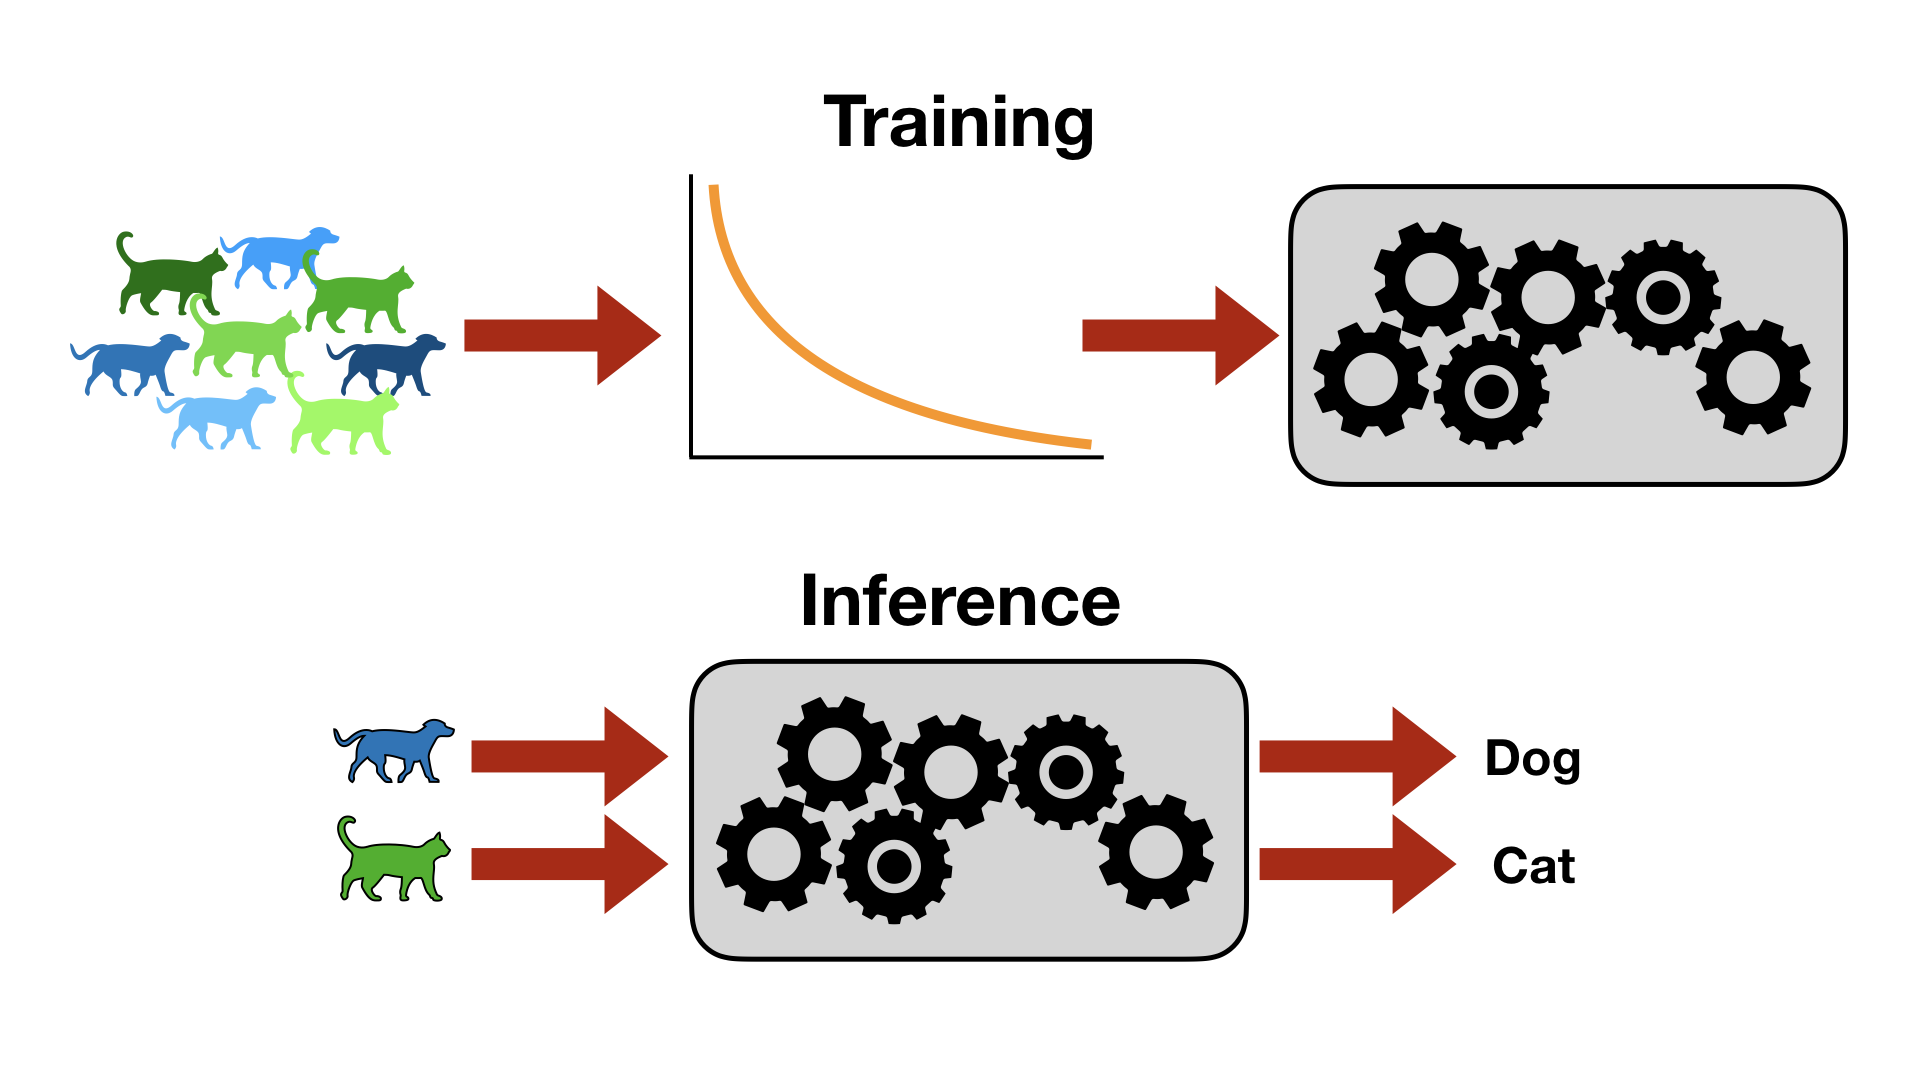
\includegraphics[trim={0 3cm 0 3cm},clip,width=0.95\textwidth]{diss/1_intro/figs/dl.png}
    \caption[Modern machine learning pipelines]{Machine learning training and inference visualization.}
    \label{fig:dl}
\end{figure}

% \textit{Explainability} can be seen as identifying important features of the input, as well as parts of the model (parameters) that ``light up`` for that input. \textit{Fairness} can be evaluated via measures over subsets of the data that correspond to specific groups. 

\begin{mdframed}[style=MyFrame]
\em 
\textbf{This thesis} focuses its main efforts on identifying these important subsets of model, feature, and sample space, to enable answering questions necessary for mainstream adoption of machine learning methods.
\end{mdframed}

% In this dissertation, we explore the sizes of these models, samples, and datasets, and 
% analyze under what situations 
% a smaller \textit{subset} of them may be sufficient or important
% for questions that run parallel to standard performance and accuracy measures.

Let us step a bit deeper into a basic illustrative example. In order to ease understanding, we can first begin with a basic formulation of learning methods, from which the questions above can take specific forms. 
Learning methods typically  try to identify a function mapping (model) that is able to complete a specific task at some high level of profficiency.
% In Figure~\ref{fig:dl}, a model is trained using examples of classification task (top), in order to accurately predict the class of a newly provided input (bottom).
% \begin{figure}
%     \centering
%     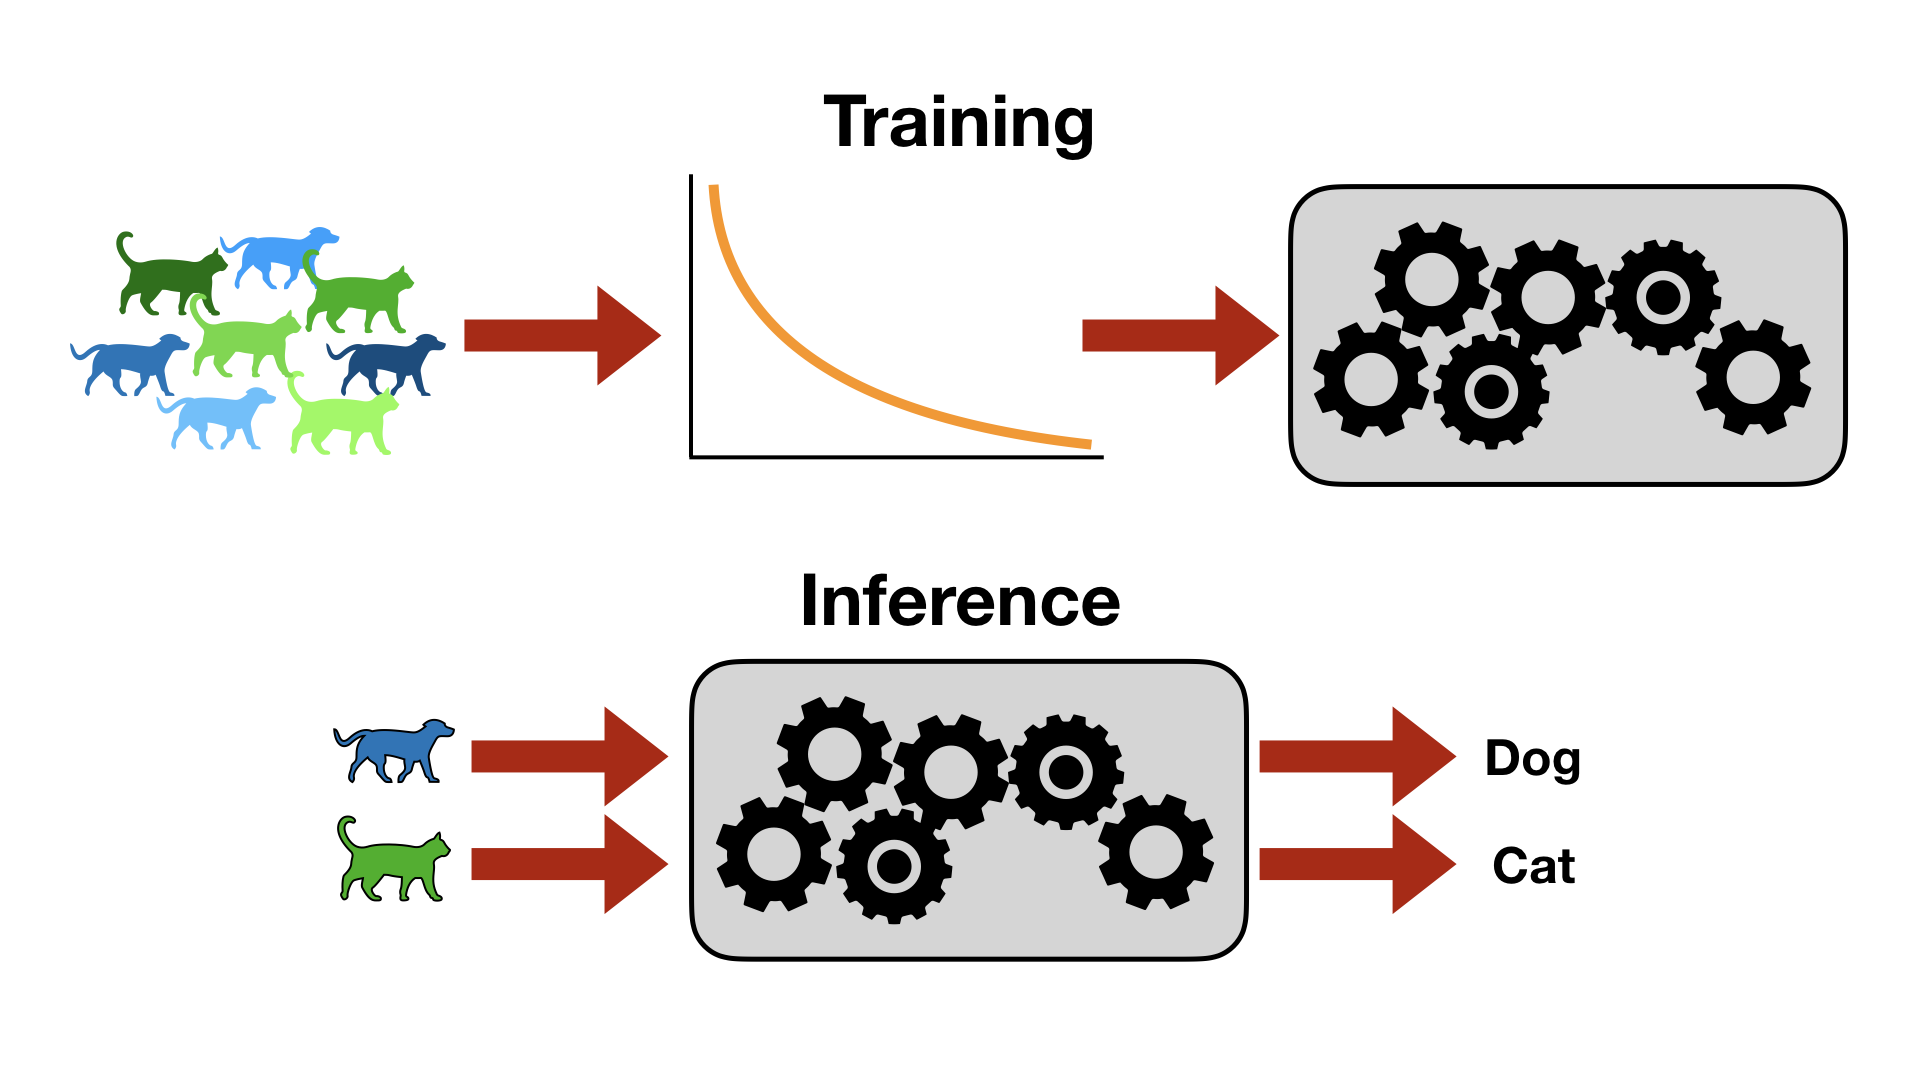
\includegraphics[trim={0 3cm 0 3cm},clip,width=0.95\textwidth]{diss/1_intro/figs/dl.png}
%     \caption[Modern machine learning pipelines]{Machine learning training and inference visualization.}
%     \label{fig:dl}
% \end{figure}
Say we have some dataset comprising of sample pairs $(x,y)$, where we wish to predict $y$ from $x$.
Our prediction, say $\hat{y}$, might be the output of some unknown function $f$ that we attempt to learn from training data. 
Let our approximation to this function be $\hat{y}:=\hat{f}(x)$.
This can take many forms, 
based on assumptions and prior information we may have on the relationships among the data. 
Consider the simple \textit{linear} case,
where we want to learn some parameter $w$ such that $y = w\cdot x$. 
Given $n$ sample pairs $(x_i,y_i)$ indexed by $i$, traditional statistics and optimization literature yield the following \textit{least squares} problem formulation, where we want to minimize the ``squared error'' between the observed values $y_i$ and the predicted $\hat{y}_i:= w\cdot x_i$:
\begin{align}\label{eq:lq}
\hat{f}:=\hat{w} = \mathop{\arg\min}_{w} \sum_{i=1}^n (y_i - w\cdot x_i)^2
\end{align}
This formulation expands without much change to a multi-dimensional form of the input $x$ and respectively, $w$: the canonical case where a number of features, or \textit{covariates} (e.g., symptoms), are used together to predict the outcome (e.g., diagnosis). 
If we are interested in which features of $x$ are important, we can look at the relative values of the learned ``weights'' $w$. In this simple setting, the importance of a feature (say $x^j$) can be exactly determined by the importance of the parameter ($w^j$).
A weight value far from zero may indicate that corresponding feature is important for diagnosis.
% If instead we are interested in which samples are most important, we can use existing methods for sample reweighting or methods that use standard assumptions to efficiently identify important subsets.

In this case and others, traditional statistical learning methods 
have been studied 
for many decades.
Linear regressors, decision trees, and support vector machines
have all been analyzed under these lenses.
% ,
% and as the modern machine learning community
% has returned to these questions recently,
% so has a renewed interest in their methods of analysis.
New research focuses
particularly on the differences
associated with moving from classical \textit{under-parametrized} models to
modern (deep) \textbf{over-parameterized} models: where
the model size vastly outnumbers the number
of input samples.
% , and may even be comparable to 
% the \textit{entire sample space.}
Methods for estimating the number of samples needed,
the time to learn a particular task,
and the generalization ability 
all require new perspectives in this regime.
While nascent, this research
attempts to fill the gap between
statistical and deep models to enable similar measures of sample influence, feature importance, and model understanding. 

\paragraph{A full picture.}
Let us expand our notation from the example above to consider this more general framing.
Consider a dataset $X:=\{x_i\}_{i=1}^n$ of size $n$ where each data point $x_i$ in the set $X$ is drawn from some underlying distribution over the domain $x_i \sim \cX^d$, 
with domain dimensionality (number of features) $d$.
A model $f$ is fit using a parametrization $\theta \in \Theta$,
with $\Theta$ the space of possible parametrizations (models) with some intrinsic dimension $p$. 
%While all three of these problems are closely related, they require different approaches. 
Generalizing the least squares``error measure'' from Eq.~\eqref{eq:lq} to an arbitrary \textit{loss} $\ell$, we have
\begin{align}\label{eq:learning}
    \hat{f}:=\hat{\theta} = \mathop{\arg\min}_{\theta\in\Theta} \sum_{x \in X} \ell(f_\theta(x_i))
\end{align}
From an analysis perspective, 
we might be interested in any one of 
(a) subsets of input features $\cC \subseteq \cX$ that are important for the downstream task,
(b) associating model subsets $\cP \subseteq \Theta$ with specific inputs or groups of inputs, or 
(c) subsets or subgroups of samples $S \subseteq \{X\}$ that are sufficient or representative of the entire dataset.

Crucially, an uninformed search for a subset is computationally infeasible. For a superset of size $n=|X|$, The set of all subsets is the power set, with a size of $2^{n}$! If an identification procedure requires looking over all of these and choosing a ``best'' one by some metric, the procedure will be limited to very small supersets.
Efficient methods have been developed in each of the three contexts above to avoid this exponential search.

\begin{figure}
    \centering
    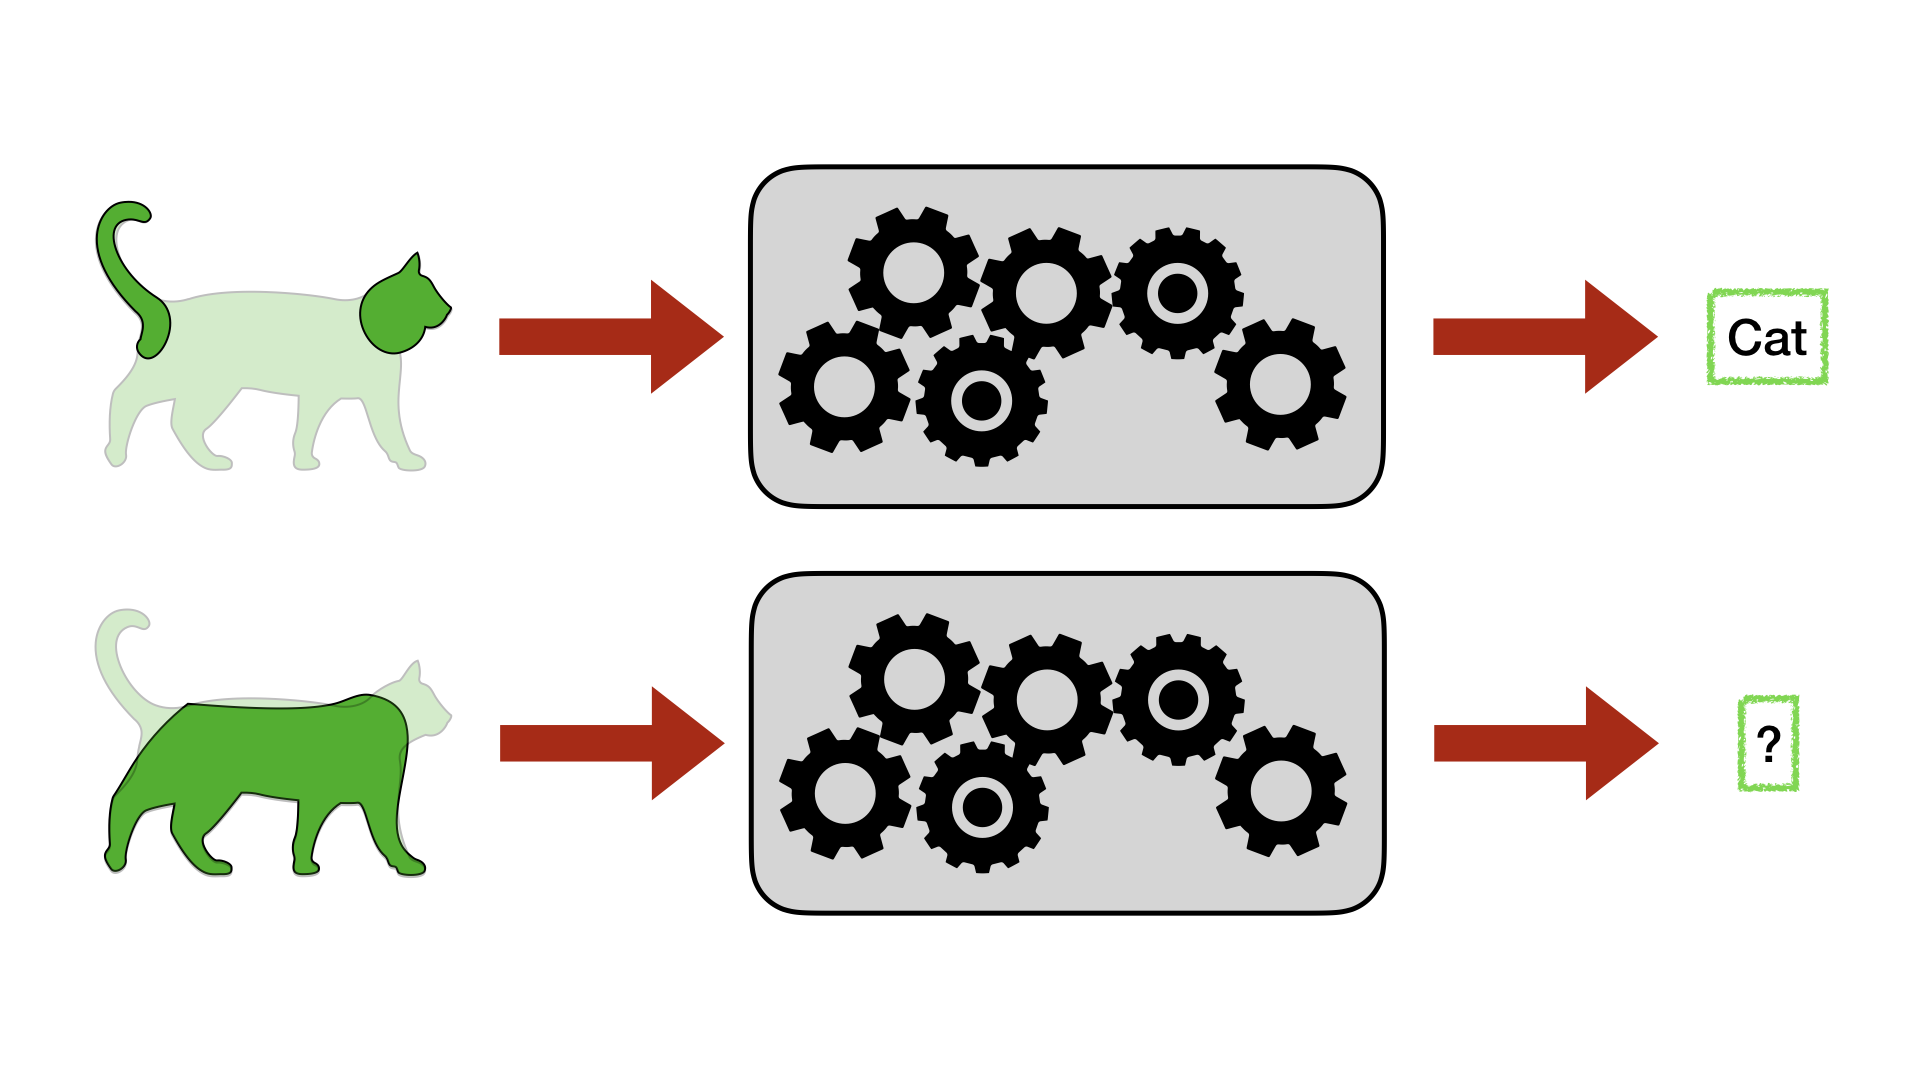
\includegraphics[trim={0 3cm 0 3cm},clip,width=0.9\textwidth]{diss/1_intro/figs/feat_select.png}
    \caption[Visualization of feature selection]{An example of identifying specific features important to the learning task.}
    \label{fig:feat_select}
\end{figure}
\paragraph{Feature Selection.} 
With more complex models $f$ compared to the linear case above, newer ``black-box'' methods have been developed for identifying important features. From the more pure statistics side, scan statistics~\citep{scanstat,scanstatlrt} allow for a structured ``scanning'' over the input space, skipping subsets unlikely to provide additional information for the measure of interest.
Further on the deep learning side, adaptations of sensitivity analysis, via noise addition and perturbations have found success~\citep{yeung2010sensitivity,zhang2015sensitivity}, alongside activation mapping~\citep{cam,selvaraju2017grad}.
These methods typically generate an analagous ``weighting'' over the input space, identifying features most salient for the specific task (Figure~\ref{fig:feat_select}).

\begin{figure}
    \centering
    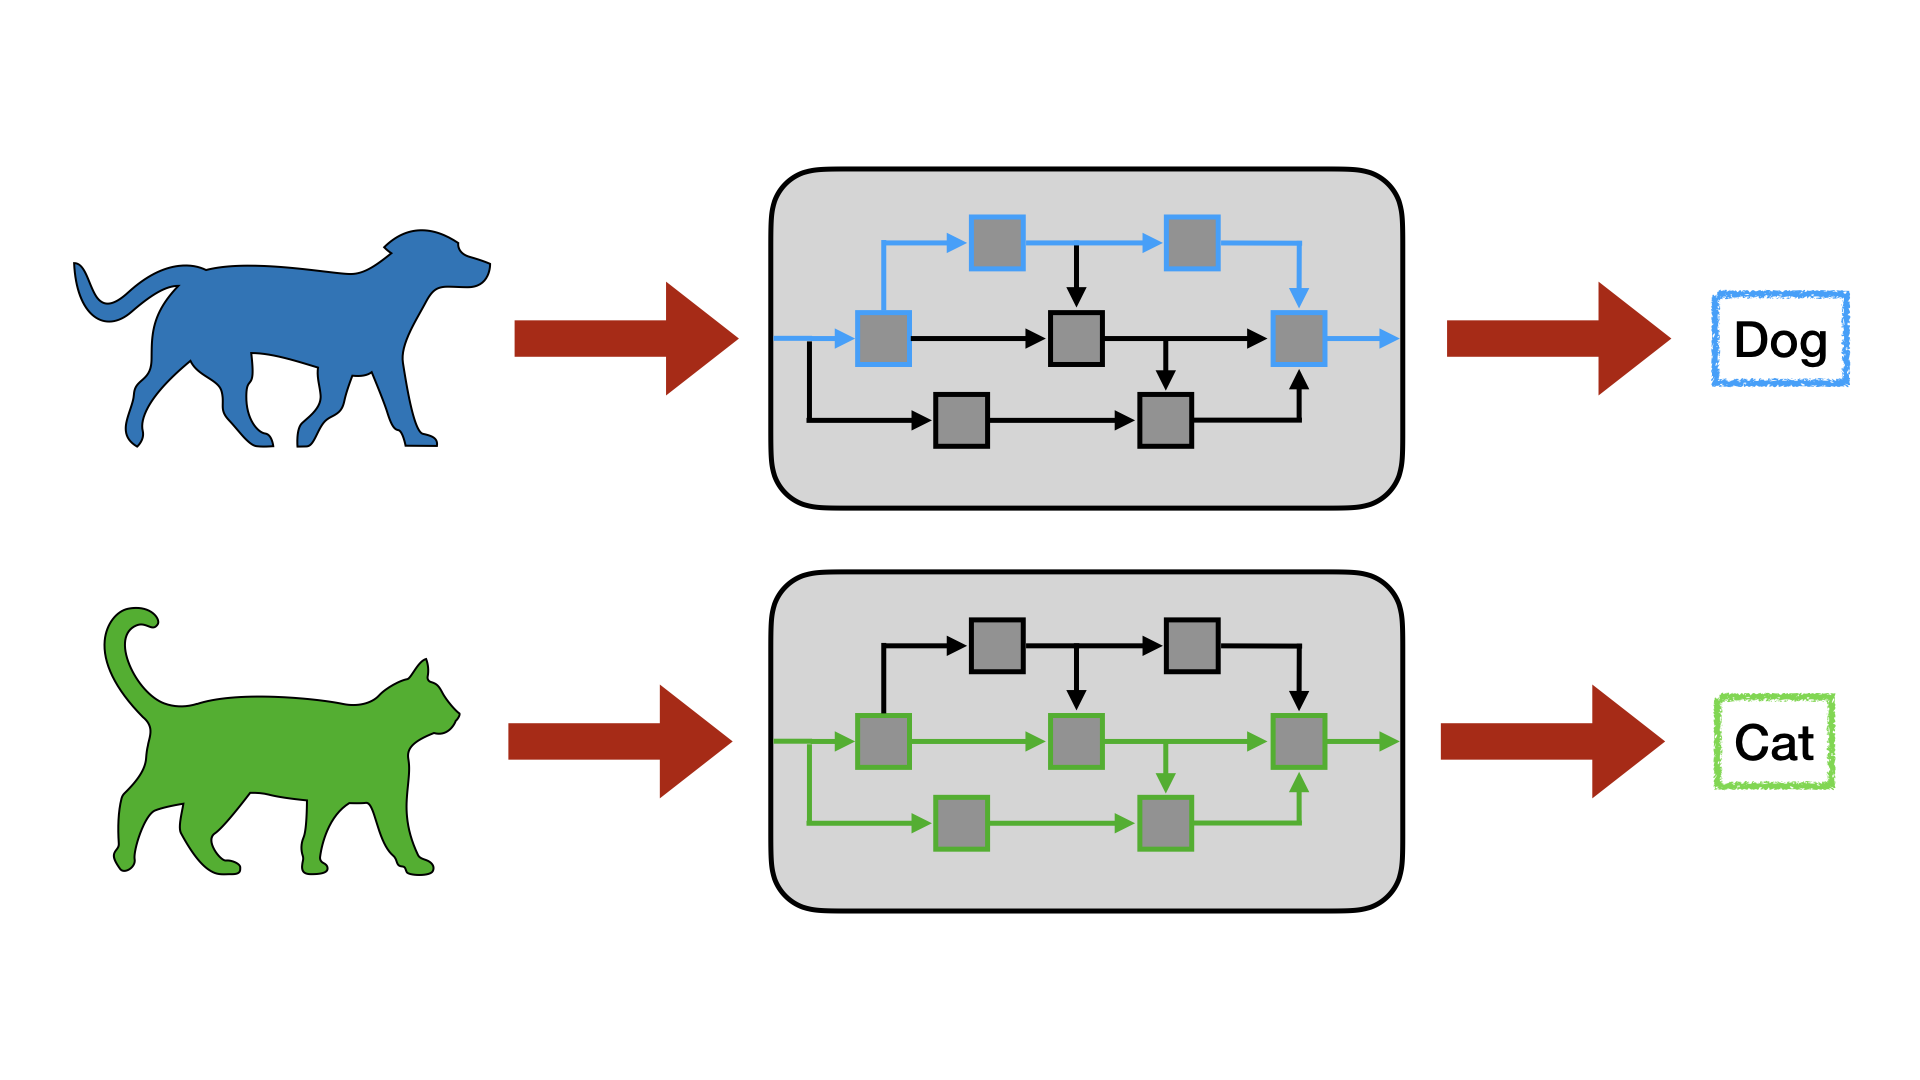
\includegraphics[trim={0 3cm 0 3cm},clip,width=0.9\textwidth]{diss/1_intro/figs/param_select.png}
    \caption[Visualization of parameter selection]{An example of identifying specific parameters important to the learning task.}
    \label{fig:param_select}
\end{figure}
\paragraph{Parameter Selection.} 
Selection in the model space generally takes two forms. First, as a prior, restriction, or assumption over the model space, and second, as a post-hoc method for an ``explainable'' proxy.
Regularization, sparsity, and gating methods are often used independent of the type or size of the model, to encourage the solution to fall within a specific region of the model space.
% In non-deep settings these methods come with strong theoretical guarantees. 
The theoretical underpinnings of these methods in deep learning are still being actively researched~\citep{hardt2016train,jacot2018neural,neyshabur2014search}, but the methods have nonetheless been effective in practice. 
On the post-hoc side, of particular interest are the parameters relevant to specific regions of the input space \textit{after} training (Figure~\ref{fig:param_select}). Here, recent analysis of deployed networks has shown this to be true~\citep{bau2017network,fong2018net2vec}, and current work continues to explore these network regions to aid in interpretability and explainability.

\paragraph{Sample Selection.} Many methods have been developed for outlier detection within training or testing sets~\citep{huang2020feature,ren2019likelihood} \textit{after} training, as well as methods for understanding sample influence~\citep{koh2017understanding,golatkar2020eternal,huang2020feature} . ``In-the-loop'' methods for accounting for ``outlierness'' behave similarly to accounting for group or individual fairness while training~\cite{mehrabi2021survey}. Unfortunately, once samples are identified in some manner, post-hoc adjustments to a trained model are generally very difficult. Recent work has focused on ``unlearning'', or removing a sample's influence on a model without retraining. If specific samples can be uniquely identified, performance and privacy reasons may require these specific interventions to reduce the ``influence'' of that sample subset.
\begin{figure}
    \centering
    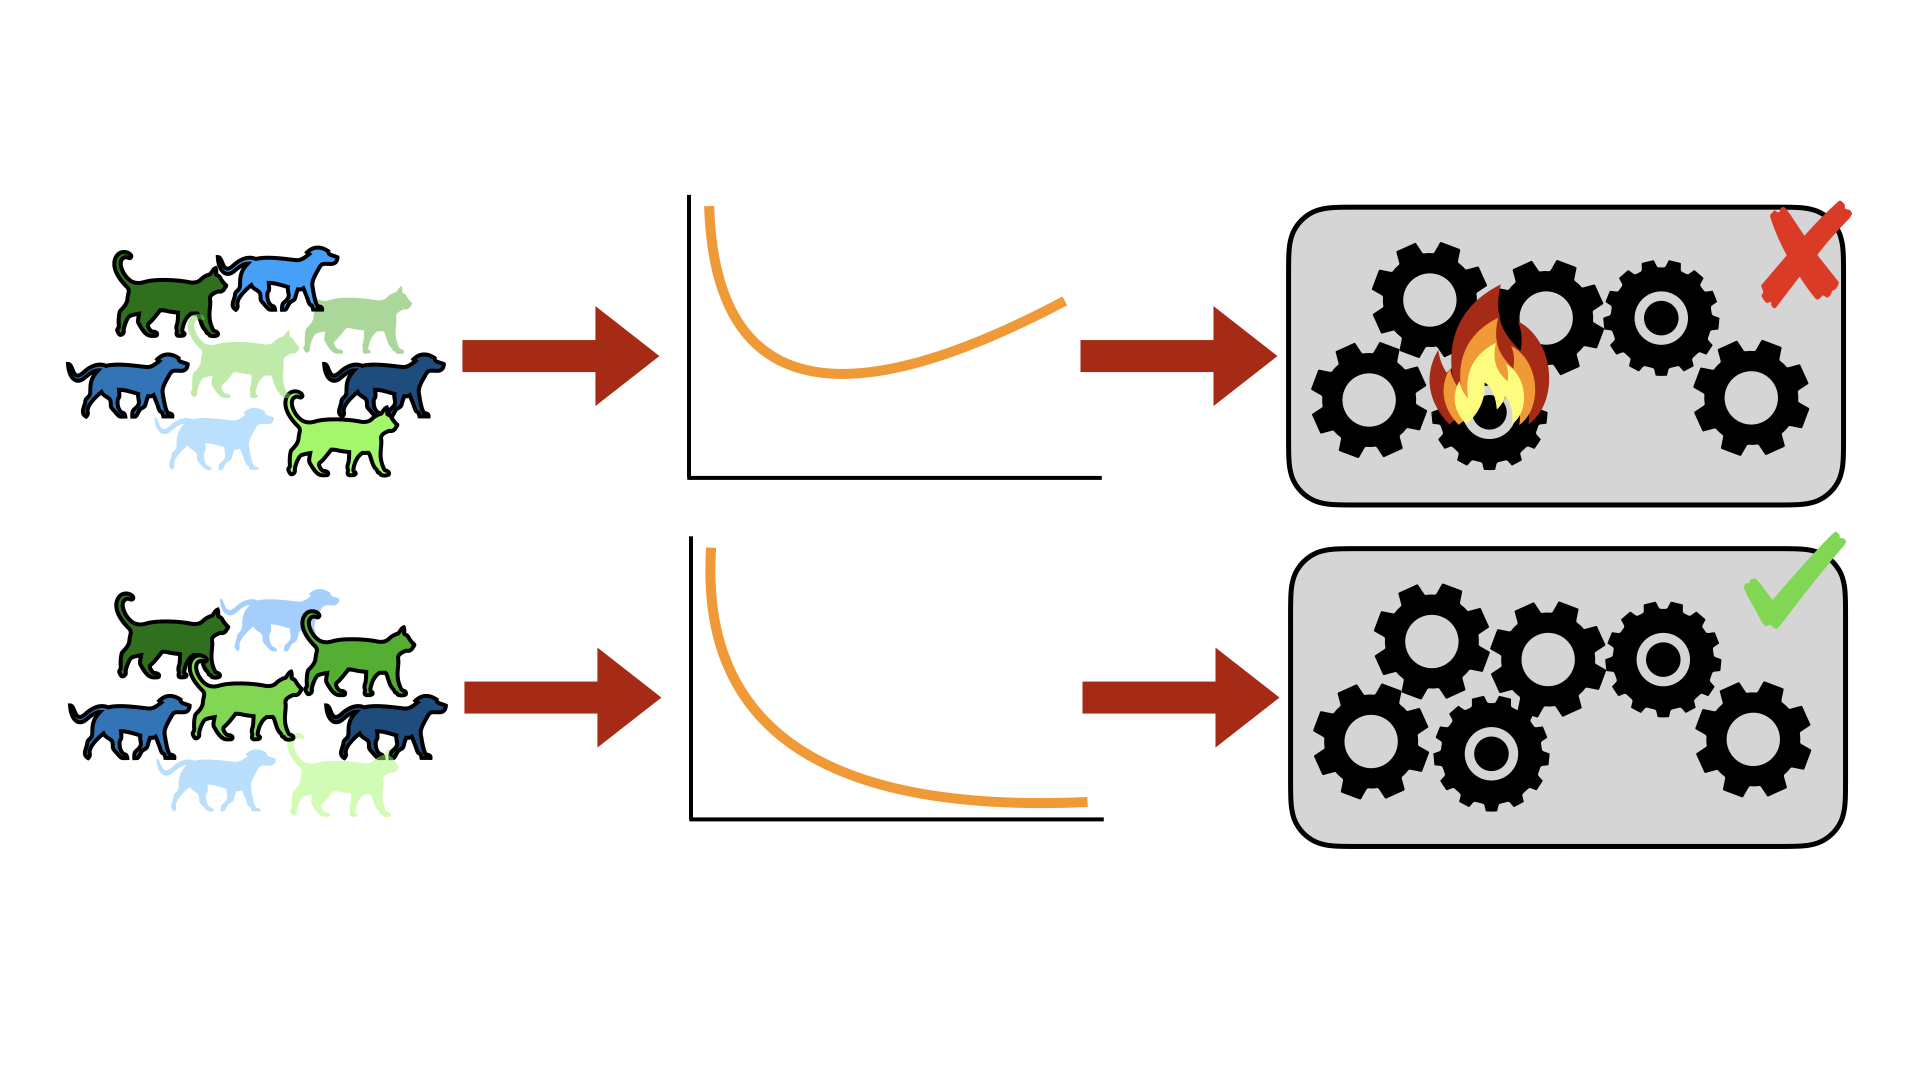
\includegraphics[trim={0 4.5cm 0 4cm},clip,width=0.9\textwidth]{diss/1_intro/figs/sample_select.png}
    \caption[Visualization of sample selection]{An example of identifying specific samples important to the learning task.}
    \label{fig:sample_select}
\end{figure}


\begin{mdframed}[style=MyFrame]
\textbf{ Thesis Goal: }
\em Identify, construct, and evaluate methods for \textbf{efficient} subset identification in modern machine learning feature, model, and input spaces.
\end{mdframed}

\section{A Few Motivating Examples}
Consider a traditional machine learning classification task in which we would like to predict whether an individual has a specific disease condition based on a medical resonance image (MRI) scan of their brain. Our input feature $x$ may consist of a 3D-array of values in $\RR^{\cI\times \cJ\times \cK}$ measuring some intensity of the imaging modality at each voxel, indexed by a tuple $(i,j,k) \in (\cI,\cJ,\cK)$.
Our outcome variable $y$ may simply be a binary label of whether the input scan has been labeled by a radiologist as one demonstrating typical disease characteristics.
Using an off the shelf 3D convolutional neural network with adjustments to match our input size, we can very quickly set up and train a system to predict disease presence with a high degree of accuracy.

\paragraph{Example 1.}
With a prediction for a specific scan, or predictions over a number of scans, we might be interested in identifying which regions of the brain are most important for diagnosis. These regions, $R \subset \cR:=\RR^{x\times y\times z}$, can be specific groups of pixels in the image that may correspond to known functional networks. Methods such as attention and class activation maps may work here, but there are a few issues. The number of samples available to learn a model is very small compared to the both the dimension of the input and the number of parameters in the model, i.e., $n \ll p$ and $n \ll d$. Thus it is very easy to overfit, and for areas of interest to be associated with intricacies of particular input data rather than true, real differences defined by the disease.

Furthermore, recent medical imaging studies have moved past simple difference detection: trends over time, and the ability to predict {\em future} disease development have by far become the setting of most interest.
Given an image of a healthy individual, is it possible to predict what their scan, or their future disease diagnosis, may be up to 10, 20, or more years in the future?
If a number of scans have been collected over some timeframe, can the \textit{trajectory} of the individuals' development be extrapolated to estimate progression?
As traditional models extended for temporal analysis grow in both size and complexity,
a number of subproblems explicitly related to model and input subspaces arise. In this thesis we address two such problems: \textbf{statistically rigorous identification of temporally evolving subsets}, and \textbf{characterizations of deep models that enable efficient training of recurrent models with large scale time-varying data}.
    
\paragraph{Example 2.}
With the rapid growth of AI and machine learning applications has come valid concerns regarding both guarantees of privacy.
Recent technology legislation has made the importance clear in all aspects of data use,
and particular projects and groups have demonstrated that machine learning is not independent of
this need \citep{Exposing}.
A new issue raised within this intersection is the ``right to be forgotten".
If a model has been trained with a particular users' data, 
they should have some recourse or right
to both remove their data from the training set,
and also know that the model has not learned from their data.
On the surface, this poses a significant problem for model builders
and organizations that spend large amounts
of time and resources in 
training deep learning models.

In the medical imaging example above this is especially important: with fewer samples it is more likely that information about any particular one could ``leak'', and the model's performance may degrade significantly as a relatively large percentage of it's training data is removed.
Thus tailored methods must be developed to ensure both privacy and performance, without requiring full retraining.
As we will see, 
\textbf{identification of model parameter subsets}
that are particularly important
for a particular sample's influence
in a model enables \textit{efficient machine unlearning}.

\paragraph{Example 3.}
From an alternative perspective, we may want to identify specific samples rather than have them specified a priori.
Traditionally a rigorous area of study under classical statistics, outlier detection and accounting have become a subfocus for many within the machine learning community as well \citep{golatkar2020eternal,golatkar2020forgetting,huang2020feature,ren2019likelihood}.
While subgroups of input samples may be outliers, it is more often the case that they represent known heterogeneity within the data. 
These differences may be marked using 
group information known a priori, and 
most learning tasks aim to learn tasks
in a \textit{subgroup-independent} manner.
In our disease prediction model above,
these groups could simply be stratified by the type of scanner used to acquire the image, but it could also
be a systematic difference correlated with some protected attribute. {\color{red} sentence about original brain atlas for registration being eurocentric}
This can directly lead to disparate performance and results on \textit{all} individuals outside of that group.
Optimization and regularization methods with this focus come under the umbrella of model fairness.
However, many existing methods do not scale well to larger models or as the number of subgroups grows, as is often the case when intersections of protected classes must be considered. Here we identify and construct a particular solution for \textbf{groupwise fairness that enables efficient in the loop fairness regularization}.

% What features are most important for prediction?
% Which samples were most important for my training?
% Can we understand when a model is certain or uncertain about its output?
% Are there layers in my network that have learned a particular subtask?
% Questions of robustness, bias, influence, fairness, and importance have become central questions to contemporary machine learning research \citep{doshi2017towards,mehrabi2021survey,amodei2016concrete}.
% machine learning, etc.

% Feature selection in the case of
% typical regression or classification 
% takes some form of learning parameters $\theta$ that allow for $\hat{y} = f_\theta(x)$ to be close to the true outcome of interest $y$.
% While forms of data $X := (x,y)$ may simply be continuous and real-valued, modern machine learning has greatly expanded formulations of the classical learning problem to include a wide variety of structured learning problems~\citep{nowozin2011structured}. 
% Consider the case when a high-dimensional input is used to predict an output with a highly-parametrized model. 
% Once learned, obvious questions arise as discussed above: are there specific low-dimensional spaces in either the input or the model space that are most important or necessary for the global learning problem of interest? Are there specific subspaces associated with particular subproblems of the global problem?
% The machine learning literature has come up with a number of ways to identify analogs of these spaces, 
% including extensions of sensitivity analysis to deep learning~\citep{yeung2010sensitivity,zhang2015sensitivity}, and constructing and identifying nonzero model subsets via particular model choices such as activations~\citep{selvaraju2017grad} and regularizers.
% In classical settings these are well understood: decision trees naturally provide ease of interpretibility via the information used to choose splits, and both linear and kernel support vector machines have been analyzed to provide for measures of sample importance via distances to the margin as well as feature importance via weights defining the learned hyperplane~\citep{Mitchell97}.
% Attention and saliency maps have emerged as popular new methods,
% given their ease of implementation and interpretation~\citep{sutskever2014sequence,vaswani2017attention,selvaraju2017grad}.
% By learning dimensions of a given input that are particularly important, either in a hard (binary) or soft (continuous weighting) manner, model builders are better able to understand and interpret what a model has learnt.
% The specific ideas of attention notwithstanding, many of these existing methods are far removed from traditional hypothesis testing frameworks.
% While some work has begun in this direction~\citep{tansey2018black},
% there remains a gap in direct identification of subsets and structures in these spaces that can be defined in statistically rigorous manners.

% \begin{figure}
%     \centering
%     \includegraphics[width=0.5\textwidth]{example-image-a}
%     \caption[A simple subset selection example]{\color{red} Identifying and selecting in MRIs, subset, sample, model ID.}
% \end{figure}

% \paragraph{A specific example.} 

% ------------------------------------------

% below here will be moved and arranged with the "selection" sections and here if relevant

% ------------------------------------------

% While attention can be directly applied to the network in order to identify ``hotspots" in the input space relating to the learned classification task, 
% given the high-dimensional nature of the input
% and the relatively small sample size 
% associated with medical imaging data, 
% it is very likely that an area of interest identified
% may be an intricacy of the training samples used rather than truly a region of disease signal.
% Class activation maps (CAMs) may be unclear, and can often associate with image artifacts unrelated to the scientific task~\citep{adebayo2018sanity}.
% Methods of generalization may help to increase confidence in identified regions, but statistical guarantees often remain out of reach.

% Furthermore, most recent problems associated with medical data have moved past simple difference detection: trends over time, and the ability to predict {\em future} disease development has by far become the setting of most interest.
% Given an image of a healthy individual, is it possible to predict what their scan, or their future disease diagnosis, may be up to 10, 20, or more years in the future?
% If a number of scans have been collected over some timeframe, can the \textit{trajectory} of the individuals' development be extrapolated to estimate progression?
% As traditional models extended for temporal analysis grow in both size and complexity,
% a number of subproblems explicitly related to model and input subspaces arise. Here we address two such problems: \textbf{statistically rigorous identification of temporally evolving subsets}, and \textbf{characterizations of deep models that enable efficient training of recurrent models with large scale time-varying data}.

% A sample's particular influence on model parameters aside, the identification of influential samples or subsets of samples more generally is of independent interest. 
% Traditionally a rigorous area of study under classical statistics, outlier detection and accounting have become a subfocus for many within the machine learning community as well \citep{golatkar2020eternal,golatkar2020forgetting,huang2020feature,ren2019likelihood}.
% While subgroups of input samples may be outliers, it is more often the case that they represent known heterogeneity within the data. 
% These differences are typically marked using 
% group information known a priori, and 
% most learning tasks aim to learn tasks
% in a \textit{subgroup-independent} manner.
% Optimization and regularization methods with this focus come under the umbrella of model fairness, and instead of identifying and boosting independences within the model or data, we aim to minimize them.
% However, many existing methods do not scale well as the number of subgroups grows, as is often the case when intersections of protected classes must be considered. In the sequel we identify and construct a particular solution for \textbf{groupwise fairness that enables efficient in the loop fairness regularization}.

\begin{mdframed}[style=MyFrame]
\em 
Here we focus our effort on identifying these important subsets of model, feature, and sample space for feature association, model size reduction, model unlearning, and, fairness. Specifically, taking advantage of both existing statistical and geometric methods, we develop new methods for localizing subsets in a range of settings from hypothesis testing to deep learning.
\end{mdframed}

\section{Thesis Scope and Contributions}

We explore the intersections of classical statistical and geometric constructions with modern machine learning methods. 
Figure~\ref{fig:scope} shows the overall scope projected along three axes: feature, parameter, and sample spaces.
Below we briefly introduce the main problems studied in this thesis.
\begin{figure}[!ht]
    \centering
    % \includegraphics[width=0.99\linewidth]{scope.pdf}
    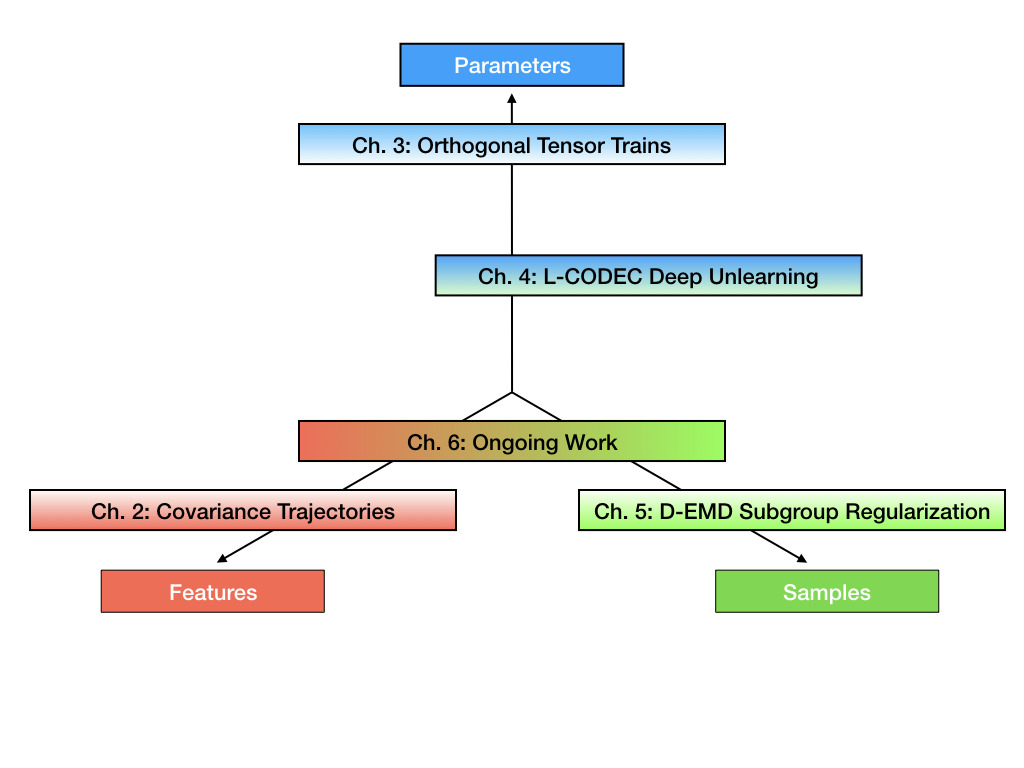
\includegraphics[width=0.95\linewidth]{diss/1_intro/figs/thesis_scope.png}
    \caption[Thesis Scope]{Thesis scope, projected over three representative axes. {\color{red} update chapter numbers shift by 1}}
    \label{fig:scope}
\end{figure}

\subsection{Second-Order Modeling and Group Difference Analysis over Time}

Recent results in coupled or temporal graphical models offer schemes for estimating the relationship structure 
between features when the data come from
related (but distinct) longitudinal sources. A novel application of these ideas is for analyzing group-level differences, i.e., in identifying if {\em trends} of estimated objects (e.g., 
covariance or precision matrices) are different across disparate conditions (e.g., gender or disease). Often, poor effect sizes make detecting the \textit{differential} signal 
over the {\em full} set of features difficult: for example, 
dependencies between only a {\em subset of features} may manifest differently across groups.
We first suggest
a parametric model 
for estimating trends in the space of $\SPD$ matrices as a function of one or more covariates.
We will then generalize scan statistics to graph structures, 
to search over distinct subsets of features (graph partitions) whose temporal dependency structure may show statistically 
significant group-wise differences.
We will theoretically analyze the Family Wise Error Rate (FWER) and bounds on Type 1 and Type 2 error. 
On a cohort of individuals with risk factors for Alzheimer's disease (but otherwise cognitively healthy), 
we 
find scientifically interesting 
group differences where the default analysis, 
i.e., models estimated on the full set of features, do not survive reasonable 
significance thresholds. 
% Preliminary work on this was published in \citep{covtraj}.


\subsection{Efficient Tensor Representations for Feasible Temporal Deep Learning}

Modern deep networks have proven to be very effective for analyzing real world images.
However, their application in medical imaging is still in its early stages,
primarily due to the large dimension of three-dimensional images, requiring enormous convolutional or fully connected layers --
if we treat an image (and not image patches) as a sample. 
These issues only compound when the focus moves towards longitudinal analysis
through recurrent structures, and when a point estimate of model parameters is insufficient 
in scientific applications where a reliability measure is necessary.
Using insights from differential geometry, 
we will adapt 
the tensor train decomposition to construct networks
with significantly fewer parameters,
allowing us to train powerful recurrent networks on whole brain image volumes. 
We analyze 
the \textit{orthogonal tensor train},
and demonstrate its ability to express a standard network layer both theoretically and empirically.
We 
demonstrate its ability to 
effectively reconstruct whole brain volumes
with faster convergence and stronger confidence intervals
compared to the standard tensor train decomposition. 
We provide code and show experiments on the ADNI dataset
using image sequences to regress on a cognition related outcome.
% Preliminary work on this was published in \citep{ott}.

\subsection{Practical Unlearning via Large-Scale Conditional Independence Testing}

%With AI systems extensively using personal %data for model training, 
Recent legislation has
led to interest in {\em machine unlearning}, i.e., removing specific training samples from a {\em predictive} model as if they never existed in the training dataset. 
Unlearning may also be required due to  corrupted/adversarial data or simply a user's updated privacy requirement.
For models which require no training ($k$-NN), 
simply deleting the closest original sample can be effective. 
%However, it is not clear how such approaches can be used to unlearn 
%models that contain rich information learned from the original data.
But this idea is inapplicable to models which learn richer 
representations.
%from data. 
%Recently, optimization-based unlearning estimators have been proposed, but 5their 
Recent ideas leveraging optimization-based updates
scale poorly with the model dimension $d$,  
due to 
inverting the Hessian of the loss function. %with an overall cost of $O(d^3)$ 
%is prohibitive.
We describe
a variant of a new conditional independence coefficient, 
L-CODEC, to identify a subset of the model parameters with the most semantic overlap on an individual sample level. 
Our approach completely avoids the need to invert a (possibly) huge matrix. 
By utilizing a Markov blanket selection, 
we find
that L-CODEC is also suitable for deep unlearning,
as well as other applications in vision.
Compared to alternatives, L-CODEC makes approximate unlearning possible 
in settings that would otherwise be infeasible, 
including vision models used for face recognition, 
person re-identification 
and NLP models that may require unlearning samples identified for exclusion.
% Preliminary work on this will appear in \citep{lcodec}.


\subsection{Reducing Subgroup Fairness via High Dimensional Earth Mover's Distances}

Optimal transport has recently emerged as a useful tool for machine learning through its connections with geometry, statistical machine learning, and through practical algorithms. Existing methods that leverage optimal transport often  regularize using  a Wasserstein metric or by computing barycenters, for example. %which are effective when distributions are continuous and known, or when measures of interest are discrete.
% Our formulation allows for a discretization of continuous measures that drop in directly to classical  formulations of the Earth Mover's Distance. 
We leverage optimal transport, except that we take advantage of a recently-introduced algorithm that computes a generalized earth mover's distance.
Not only is this algorithm computationally cheaper to compute compared to existing barycentric measures, but our method has the additional  advantage that gradients used for backpropagation can be directly read off of the forward pass computation, which leads to substantially faster model training.
We provide technical details about this new regularization term and its properties, 
and 
experimental demonstrations of improved training speed over existing Wasserstein-style methods.

{\color{red}
\subsection{Understanding Latent Spaces via Conditional Independences}

The final chapter of this thesis applies some of the tools developed above in the analysis of latent spaces in recent large scale models.
% In these studies, 
% we aim to identify conditionally independent features and subjects that are particularly important to the prediction and estimation of
% key disease outcomes,
% as a function of a number 
% of demographic, neuropsychological,
% genetic,
% and imaging data collected as 
% part of an ongoing consortium 
% to understand the progression
% of Alzheimer's disease in younger, 
% asymptomatic populations.
% In what follows we present
% exploratory analysis
% on a small, easily 
% digestible subset of the available data,
% that lays the foundation for
% further analysis.
}
% This work is the most forward looking, and aims to be a stepping stone toward a rigorous 

\section{Outline}
Chapter 2 covers the essential background necessary for the developments presented in the following chapters, including specifics of graphs and hypothesis testing, as well as relevant modern methods for learning and optimization.
In Chapters 3 through 7, we describe four perspectives to address subset identification.
Chapter 3 explores and focuses on the identification of feature subsets varying over time.
In Chapter 4 we describe a method of constraining the parameter space in a particular manner
that enables more efficient large scale neural networks.
Next, Chapter 5 provides a solution to the machine unlearning problem,
enabled through a particular conditional independence parameter selection scheme, vastly reducing network update costs.
Chapter 6 ends with a unique solution to subgroup fairness, 
where we take advantage of an efficient solution to
the $d$-dimensional earth mover's problem
to regularize large models when the number of subgroups can be large.
{\color{red} Chapter 7 describes future work, focused on applying a particular solution from Chapter 5 to understanding relationships among features in latent spaces learned by large generative models.}


%%%%%%%%%%%%% 
% Some old stuff

% Significant progress in the modern development of machine learning has
% been built upon connections and patterns identified across myriad
% interdisciplinary fields of study.
% Up through the mid 2000's, 
% many of these methods were inspired by and interested in 
% highly focused and constrained problems. 
% With a reasonably sized input domain, could a model of roughly equal size be used to
% predict some output?
% Linear regressors, decision trees, and support vector machines were all answers to these questions, with their own
% varying degrees of scaling and complexity.
% These methods necessitated carefully constructed formulations with specific restrictions to the learnable function class,
% enabling straightforward analysis 
% for provable performance guarantees 
% and easy identification of critical training samples and important input features.

% Contemporary machine learning, however, has a vastly different modus operandi. 
% Driven in large part by the exponential growth of available computation via Moore's Law, \textit{deep learning} has fallen squarely in the realm of \textbf{over-parameterized} models.
% With these overparametrizations and computation capacity, the typical learning questions posed as maximizing accuracy or reducing error have largely been addressed for even large scale problems.
% As such, complementary questions have led to subfields focusing on other performance measures, such as robustness, fairness, interpretability, and explainability.
% Many solutions to these questions end up looking back at answers found for the under- or non-parametrized settings.
% While nascent, these approaches 
% attempt to fill the gap between
% statistical and deep models to enable similar measures of sample influence, feature importance, and model analysis. 
% Most notable amongst these newer approaches is that of (Self)-Attention in Neural Networks \citep{sutskever2014sequence,vaswani2017attention}.
% Other proposals 
% end up looking back at the types of analysis typical of those more classical under-parametrized or nonparametrized methods.

% Not limited to previous developments in learning or computation theory, the arguably most valuable contributions toward the exponential reduction in model error can be attributed to influences and intuitions taken
% from biology, psychology, neuroscience, and even XXX \citep{srivastava, etc}.
% Perhaps one explanation as to why this phenomenon exists may be attributed to the way in which deep learning evolved. 
% The classical learning goal of function approximation lends itself nicely to a system which allows for arbitrary complexity via simple changes (e.g., addition of neural network layers). % Foundational works building on the original neural networks particularly have taken advantage of constraining this space of functions to search over: 
% the most seminal case being those of convolutional filters for imaging data. 
% While ``constraints" of this form have helped tremendously in model performance on modern vision and language machine learning tasks (GANs, Recurrent Networks, Residual Layers, Transformers, etc.), the ability to identify \textit{subsets} of important samples, input features, and model parameters has lagged significantly behind the development of these methods.
% Recently larger interest has been taken by the community to understand and interpret models with this view, only after extremely large and opaque models have become ubiquitous.
%This lag directly explains the more recent interest in developing methods for understanding and interpreting large scale machine learning models.
\chapter{Introduction} \label{chap:intro} 

Modern applications of machine learning in a broad range of industrial and consumer-facing systems have become ubiquitous.
Most interactions with daily technologies now intrinsically involve 
a request to some ``smart`` system in the ``cloud'', 
where those interactions range from
a request for map directions 
to simply loading a webpage.
Neural network models, and the recent advances of deep learning,
have enabled these systems that 
make such applications possible.
These models have achieved
human-level performance on learning tasks
including image classification~\citep{resnet,alexnet}, image segmentation~\citep{segmentation}, video analysis~\citep{zhang2016video}, text understanding and generation~\citep{bert,gpt}, and have slowly begun to solve more fundamental scientific problems such as protein folding~\citep{protein} drug discovery~\citep{drugdisc}, and medical diagnosis~\citep{diag}.
While this performance is largely attributed to model size,
the abundance of high quality training data
has equally contributed to real world performance,
enabling model training over millions of real world samples~\citep{imagenet,laion},
and potentially billions of synthetic samples via environment simulation~\citep{mcts}.

While deployment in some domains (recommender systems, object detection) may benefit almost unconditionally from this vastly expanded capability, rightful hesitancy has limited their widespread use in particular applications where impacts on individuals, people, or environments may be at stake.
These ``last mile'' concerns take a few forms.
% Because a completely accurate model is still out of reach, an important question that needs to be answered is: which inputs or individuals are being given incorrect outcomes, and why?
% maybe a sentence suggesting unlearning/removal
In mission critical applications such as medical diagnosis, 
the impact of an error can be extremely large,
even if a misprediction happens extremely infrequently.
Additionally, large scale model training and architecture search
can require exorbitant amounts of energy producing high emissions,
and their scale can limit market participants
to only large actors with vast existing resources.
The accessibility and effectiveness of these models can also vary significantly based on the training data, and disparate outcomes can be exacerbated by existing social inequity.

While existing human or ``natural'' systems that these models aim to assist are not perfect, 
our real world has developed norms and regulations that 
enable them to function.
A medical diagnosis might require a physician to explain what symptoms led them to that particular conclusion.
Energy metering and carbon taxes may be applied to limit
emissions.
Regulatory satisfaction may require 
analysis proving equal opportunity,
or that specific protected classes
are not used in decision making.
% Specifically, these can include ideas as simple as the Hippocratic Oath and medical malpractice insurance, to asking your doctor what symptoms lead them to a particular diagnosis.
These ideas are difficult to directly translate to automated machine learning systems,
but proxies have been identified that we can build upon.

These norms and regulations answer a number of questions we may also try to pose to our machine learning models.
What is the cost to learn this task?
What led to this particular outcome?
Why is this outcome different from another?
% We will explore how these questions can be formulated concretely. 

If the answer to these questions is negative or unknown,  follow-up questions all take an interesting form:
Can we learn a smaller model with similar performance? 
Can we identify the most important features? 
Which individuals or groups are being treated unfairly, and can we change that?
These questions ask us to identify a \textit{subset} of some relevant set, dependent on setting, and this identification is our focus here.

% Moving specifically to machine learning methods,
Taking a step back, let's take a look at a representative system. Figure~\ref{fig:dl} illustrates a typical learning pipeline. 
A dataset is collected and used to train a model, by minimizing the error over
those samples in the dataset (top).
A ``sample'' can be a single measured value, or it can
be a large, highly structured object with many ``features.''
The model is made up of some ``parameters'' that are 
tuned during training to learn a good predictor over the training dataset.
This model is then used to predict, or \textit{infer}, on new
data seen ``in the wild'' (bottom).
Our questions above are formally asking to identify \textit{subsets of these objects}: is a subset of the model parameters sufficient for learning? Which subset of the features are important for a prediction? Which subset of the dataset exhibit a specific attribute?
\begin{figure}
    \centering
    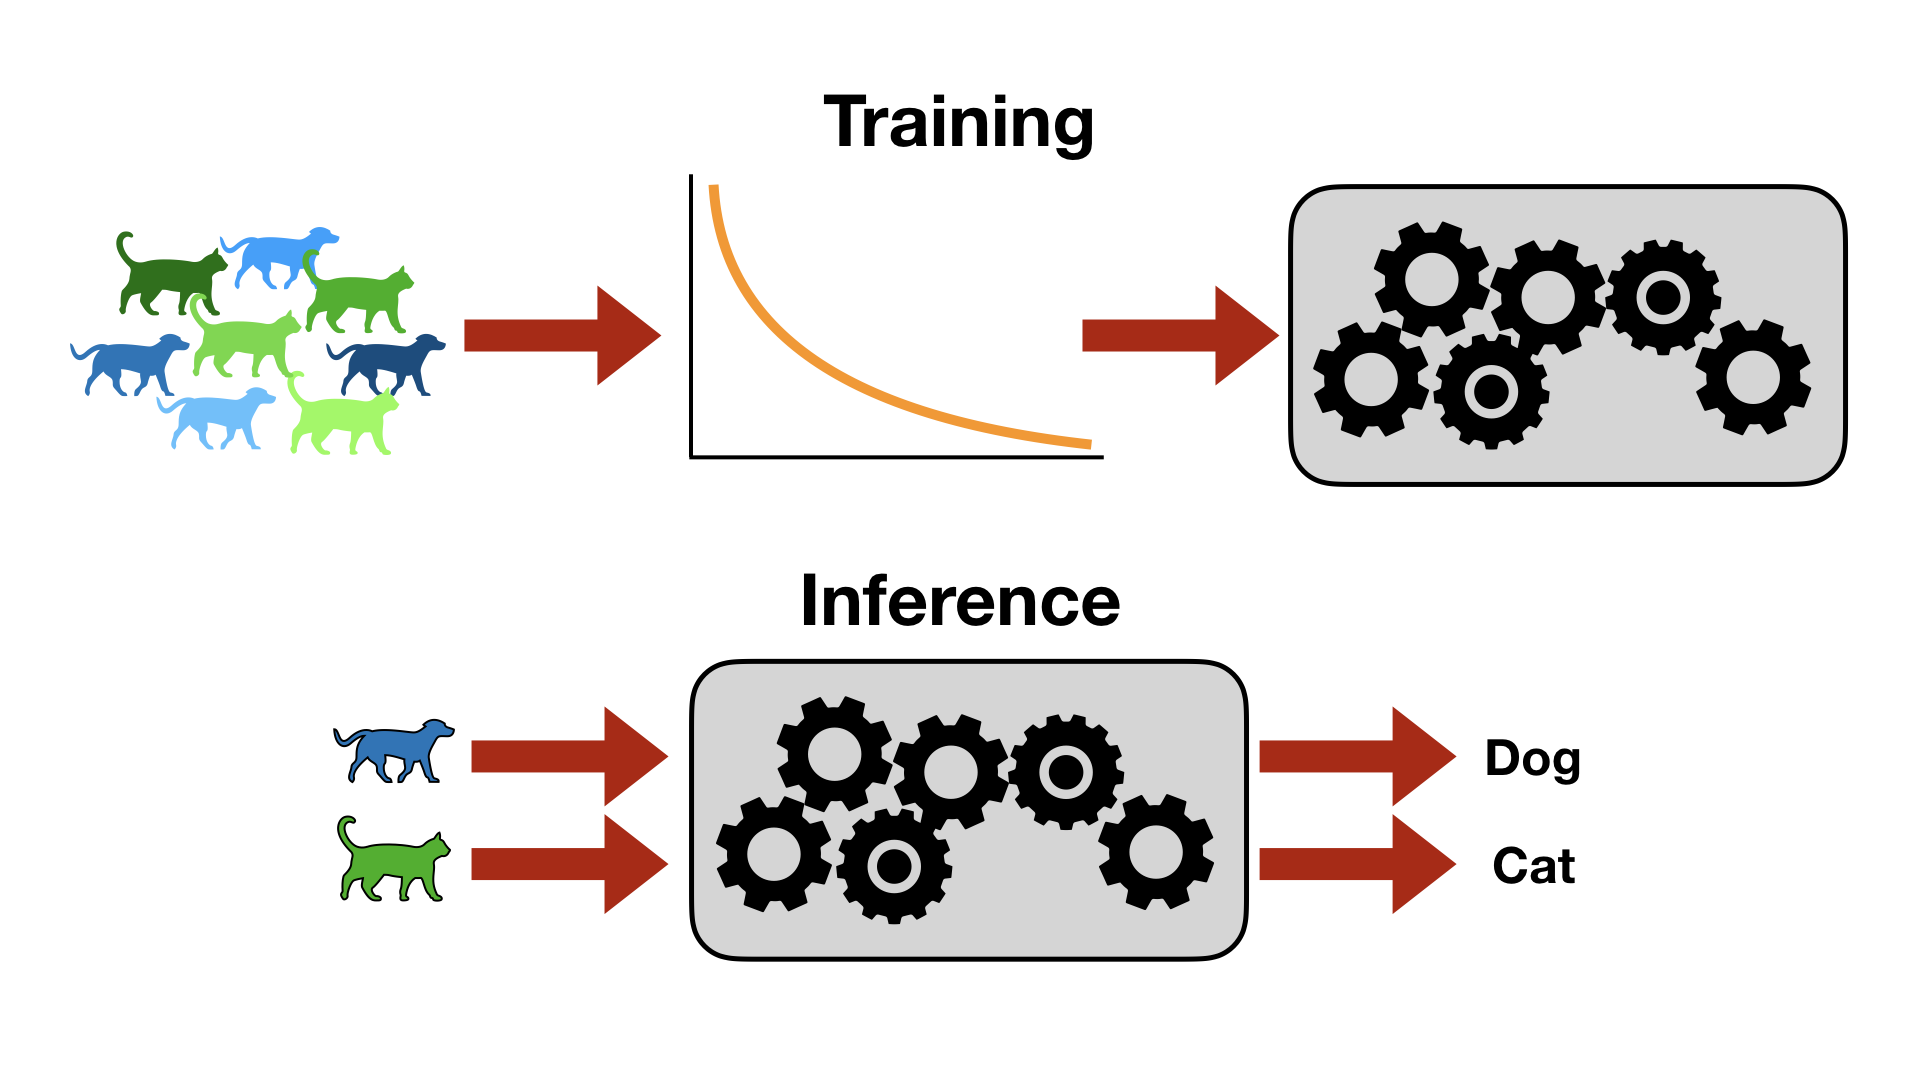
\includegraphics[trim={0 3cm 0 3cm},clip,width=0.95\textwidth]{diss/1_intro/figs/dl.png}
    \caption[Modern machine learning pipelines]{Machine learning training and inference visualization.}
    \label{fig:dl}
\end{figure}

% \textit{Explainability} can be seen as identifying important features of the input, as well as parts of the model (parameters) that ``light up`` for that input. \textit{Fairness} can be evaluated via measures over subsets of the data that correspond to specific groups. 

\begin{mdframed}[style=MyFrame]
\em 
\textbf{This thesis} focuses its main efforts on identifying these important subsets of model, feature, and sample space, to enable answering questions necessary for mainstream adoption of machine learning methods.
\end{mdframed}

% In this dissertation, we explore the sizes of these models, samples, and datasets, and 
% analyze under what situations 
% a smaller \textit{subset} of them may be sufficient or important
% for questions that run parallel to standard performance and accuracy measures.

Let us step a bit deeper into a basic illustrative example. In order to ease understanding, we can first begin with a basic formulation of learning methods, from which the questions above can take specific forms. 
Learning methods typically  try to identify a function mapping (model) that is able to complete a specific task at some high level of profficiency.
% In Figure~\ref{fig:dl}, a model is trained using examples of classification task (top), in order to accurately predict the class of a newly provided input (bottom).
% \begin{figure}
%     \centering
%     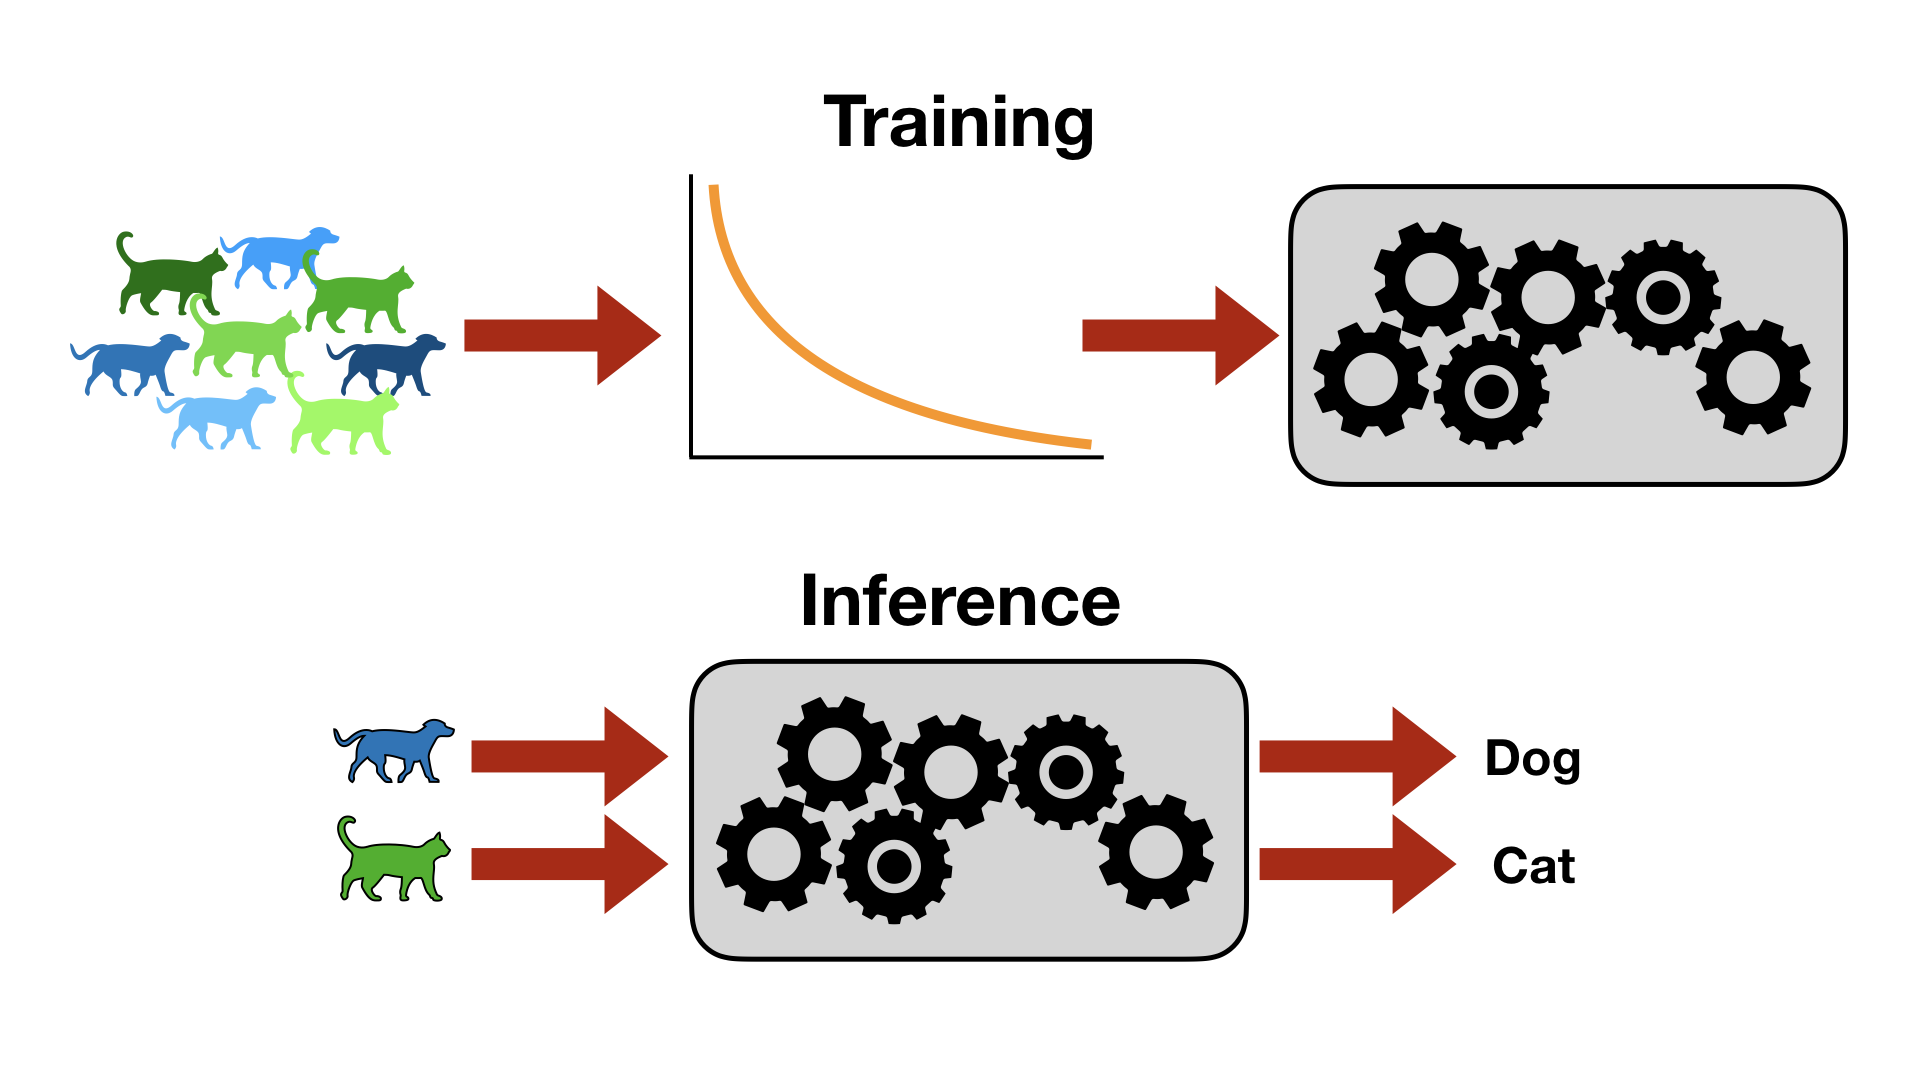
\includegraphics[trim={0 3cm 0 3cm},clip,width=0.95\textwidth]{diss/1_intro/figs/dl.png}
%     \caption[Modern machine learning pipelines]{Machine learning training and inference visualization.}
%     \label{fig:dl}
% \end{figure}
Say we have some dataset comprising of sample pairs $(x,y)$, where we wish to predict $y$ from $x$.
Our prediction, say $\hat{y}$, might be the output of some unknown function $f$ that we attempt to learn from training data. 
Let our approximation to this function be $\hat{y}:=\hat{f}(x)$.
This can take many forms, 
based on assumptions and prior information we may have on the relationships among the data. 
Consider the simple \textit{linear} case,
where we want to learn some parameter $w$ such that $y = w\cdot x$. 
Given $n$ sample pairs $(x_i,y_i)$ indexed by $i$, traditional statistics and optimization literature yield the following \textit{least squares} problem formulation, where we want to minimize the ``squared error'' between the observed values $y_i$ and the predicted $\hat{y}_i:= w\cdot x_i$:
\begin{align}\label{eq:lq}
\hat{f}:=\hat{w} = \mathop{\arg\min}_{w} \sum_{i=1}^n (y_i - w\cdot x_i)^2
\end{align}
This formulation expands without much change to a multi-dimensional form of the input $x$ and respectively, $w$: the canonical case where a number of features, or \textit{covariates} (e.g., symptoms), are used together to predict the outcome (e.g., diagnosis). 
If we are interested in which features of $x$ are important, we can look at the relative values of the learned ``weights'' $w$. In this simple setting, the importance of a feature (say $x^j$) can be exactly determined by the importance of the parameter ($w^j$).
A weight value far from zero may indicate that corresponding feature is important for diagnosis.
% If instead we are interested in which samples are most important, we can use existing methods for sample reweighting or methods that use standard assumptions to efficiently identify important subsets.

In this case and others, traditional statistical learning methods 
have been studied 
for many decades.
Linear regressors, decision trees, and support vector machines
have all been analyzed under these lenses.
% ,
% and as the modern machine learning community
% has returned to these questions recently,
% so has a renewed interest in their methods of analysis.
New research focuses
particularly on the differences
associated with moving from classical \textit{under-parametrized} models to
modern (deep) \textbf{over-parameterized} models: where
the model size vastly outnumbers the number
of input samples.
% , and may even be comparable to 
% the \textit{entire sample space.}
Methods for estimating the number of samples needed,
the time to learn a particular task,
and the generalization ability 
all require new perspectives in this regime.
While nascent, this research
attempts to fill the gap between
statistical and deep models to enable similar measures of sample influence, feature importance, and model understanding. 

\paragraph{A full picture.}
Let us expand our notation from the example above to consider this more general framing.
Consider a dataset $X:=\{x_i\}_{i=1}^n$ of size $n$ where each data point $x_i$ in the set $X$ is drawn from some underlying distribution over the domain $x_i \sim \cX^d$, 
with domain dimensionality (number of features) $d$.
A model $f$ is fit using a parametrization $\theta \in \Theta$,
with $\Theta$ the space of possible parametrizations (models) with some intrinsic dimension $p$. 
%While all three of these problems are closely related, they require different approaches. 
Generalizing the least squares``error measure'' from Eq.~\eqref{eq:lq} to an arbitrary \textit{loss} $\ell$, we have
\begin{align}\label{eq:learning}
    \hat{f}:=\hat{\theta} = \mathop{\arg\min}_{\theta\in\Theta} \sum_{x \in X} \ell(f_\theta(x_i))
\end{align}
From an analysis perspective, 
we might be interested in any one of 
(a) subsets of input features $\cC \subseteq \cX$ that are important for the downstream task,
(b) associating model subsets $\cP \subseteq \Theta$ with specific inputs or groups of inputs, or 
(c) subsets or subgroups of samples $S \subseteq \{X\}$ that are sufficient or representative of the entire dataset.

Crucially, an uninformed search for a subset is computationally infeasible. For a superset of size $n=|X|$, The set of all subsets is the power set, with a size of $2^{n}$! If an identification procedure requires looking over all of these and choosing a ``best'' one by some metric, the procedure will be limited to very small supersets.
Efficient methods have been developed in each of the three contexts above to avoid this exponential search.

\begin{figure}
    \centering
    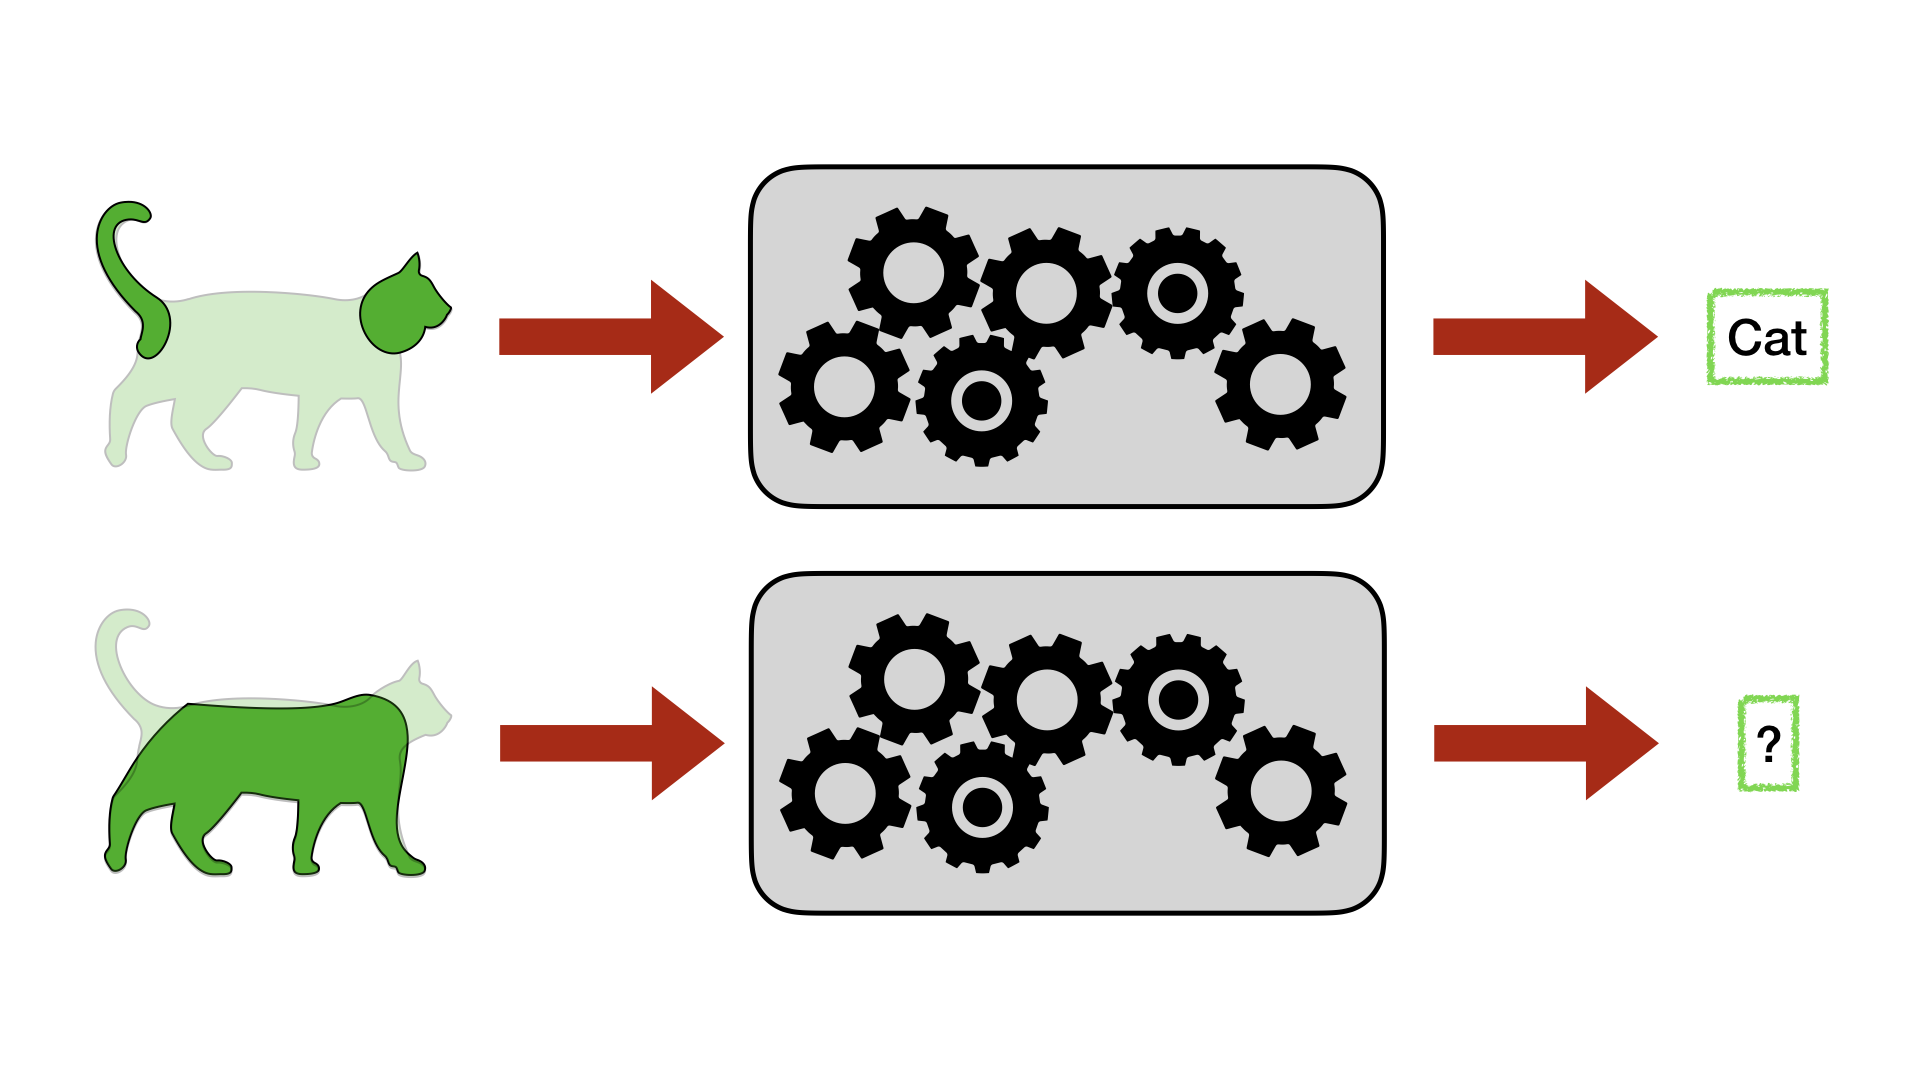
\includegraphics[trim={0 3cm 0 3cm},clip,width=0.9\textwidth]{diss/1_intro/figs/feat_select.png}
    \caption[Visualization of feature selection]{An example of identifying specific features important to the learning task.}
    \label{fig:feat_select}
\end{figure}
\paragraph{Feature Selection.} 
With more complex models $f$ compared to the linear case above, newer ``black-box'' methods have been developed for identifying important features. From the more pure statistics side, scan statistics~\citep{scanstat,scanstatlrt} allow for a structured ``scanning'' over the input space, skipping subsets unlikely to provide additional information for the measure of interest.
Further on the deep learning side, adaptations of sensitivity analysis, via noise addition and perturbations have found success~\citep{yeung2010sensitivity,zhang2015sensitivity}, alongside activation mapping~\citep{cam,selvaraju2017grad}.
These methods typically generate an analagous ``weighting'' over the input space, identifying features most salient for the specific task (Figure~\ref{fig:feat_select}).

\begin{figure}
    \centering
    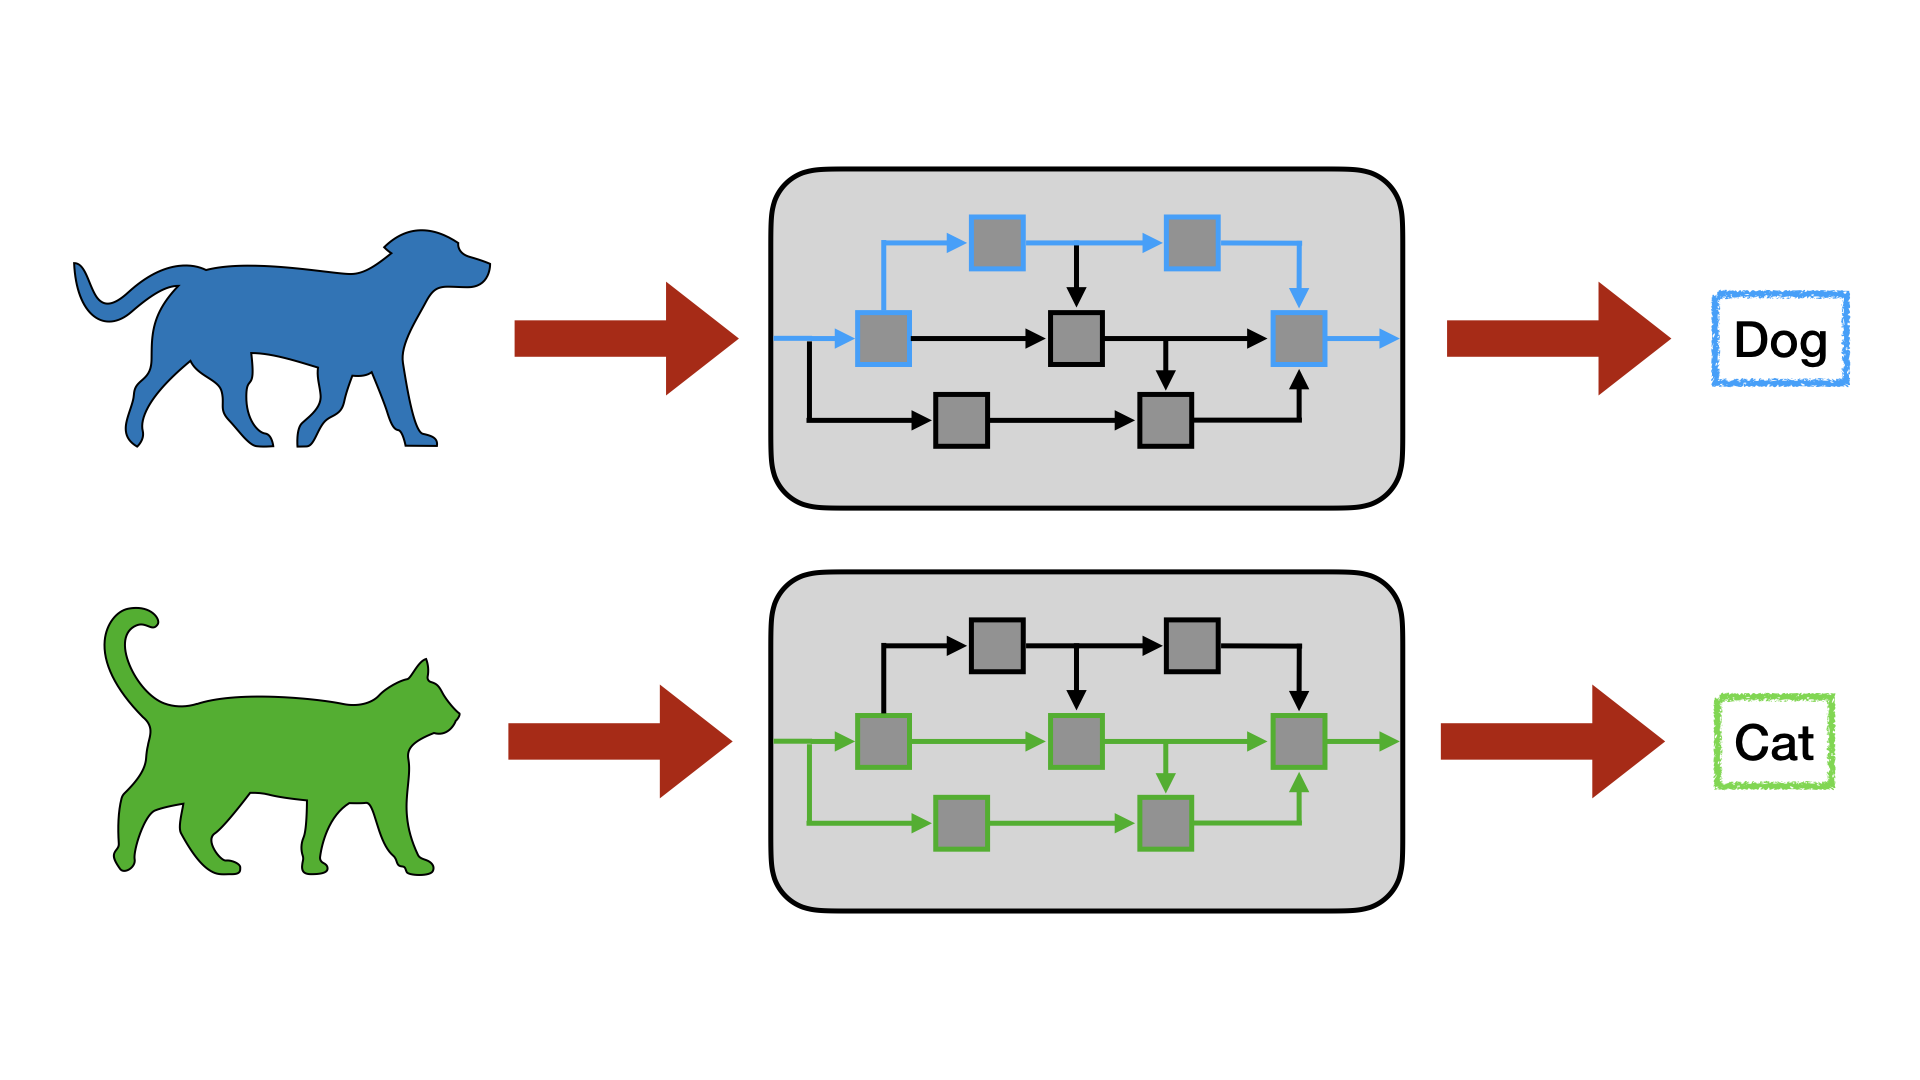
\includegraphics[trim={0 3cm 0 3cm},clip,width=0.9\textwidth]{diss/1_intro/figs/param_select.png}
    \caption[Visualization of parameter selection]{An example of identifying specific parameters important to the learning task.}
    \label{fig:param_select}
\end{figure}
\paragraph{Parameter Selection.} 
Selection in the model space generally takes two forms. First, as a prior, restriction, or assumption over the model space, and second, as a post-hoc method for an ``explainable'' proxy.
Regularization, sparsity, and gating methods are often used independent of the type or size of the model, to encourage the solution to fall within a specific region of the model space.
% In non-deep settings these methods come with strong theoretical guarantees. 
The theoretical underpinnings of these methods in deep learning are still being actively researched~\citep{hardt2016train,jacot2018neural,neyshabur2014search}, but the methods have nonetheless been effective in practice. 
On the post-hoc side, of particular interest are the parameters relevant to specific regions of the input space \textit{after} training (Figure~\ref{fig:param_select}). Here, recent analysis of deployed networks has shown this to be true~\citep{bau2017network,fong2018net2vec}, and current work continues to explore these network regions to aid in interpretability and explainability.

\paragraph{Sample Selection.} Many methods have been developed for outlier detection within training or testing sets~\citep{huang2020feature,ren2019likelihood} \textit{after} training, as well as methods for understanding sample influence~\citep{koh2017understanding,golatkar2020eternal,huang2020feature} . ``In-the-loop'' methods for accounting for ``outlierness'' behave similarly to accounting for group or individual fairness while training~\cite{mehrabi2021survey}. Unfortunately, once samples are identified in some manner, post-hoc adjustments to a trained model are generally very difficult. Recent work has focused on ``unlearning'', or removing a sample's influence on a model without retraining. If specific samples can be uniquely identified, performance and privacy reasons may require these specific interventions to reduce the ``influence'' of that sample subset.
\begin{figure}
    \centering
    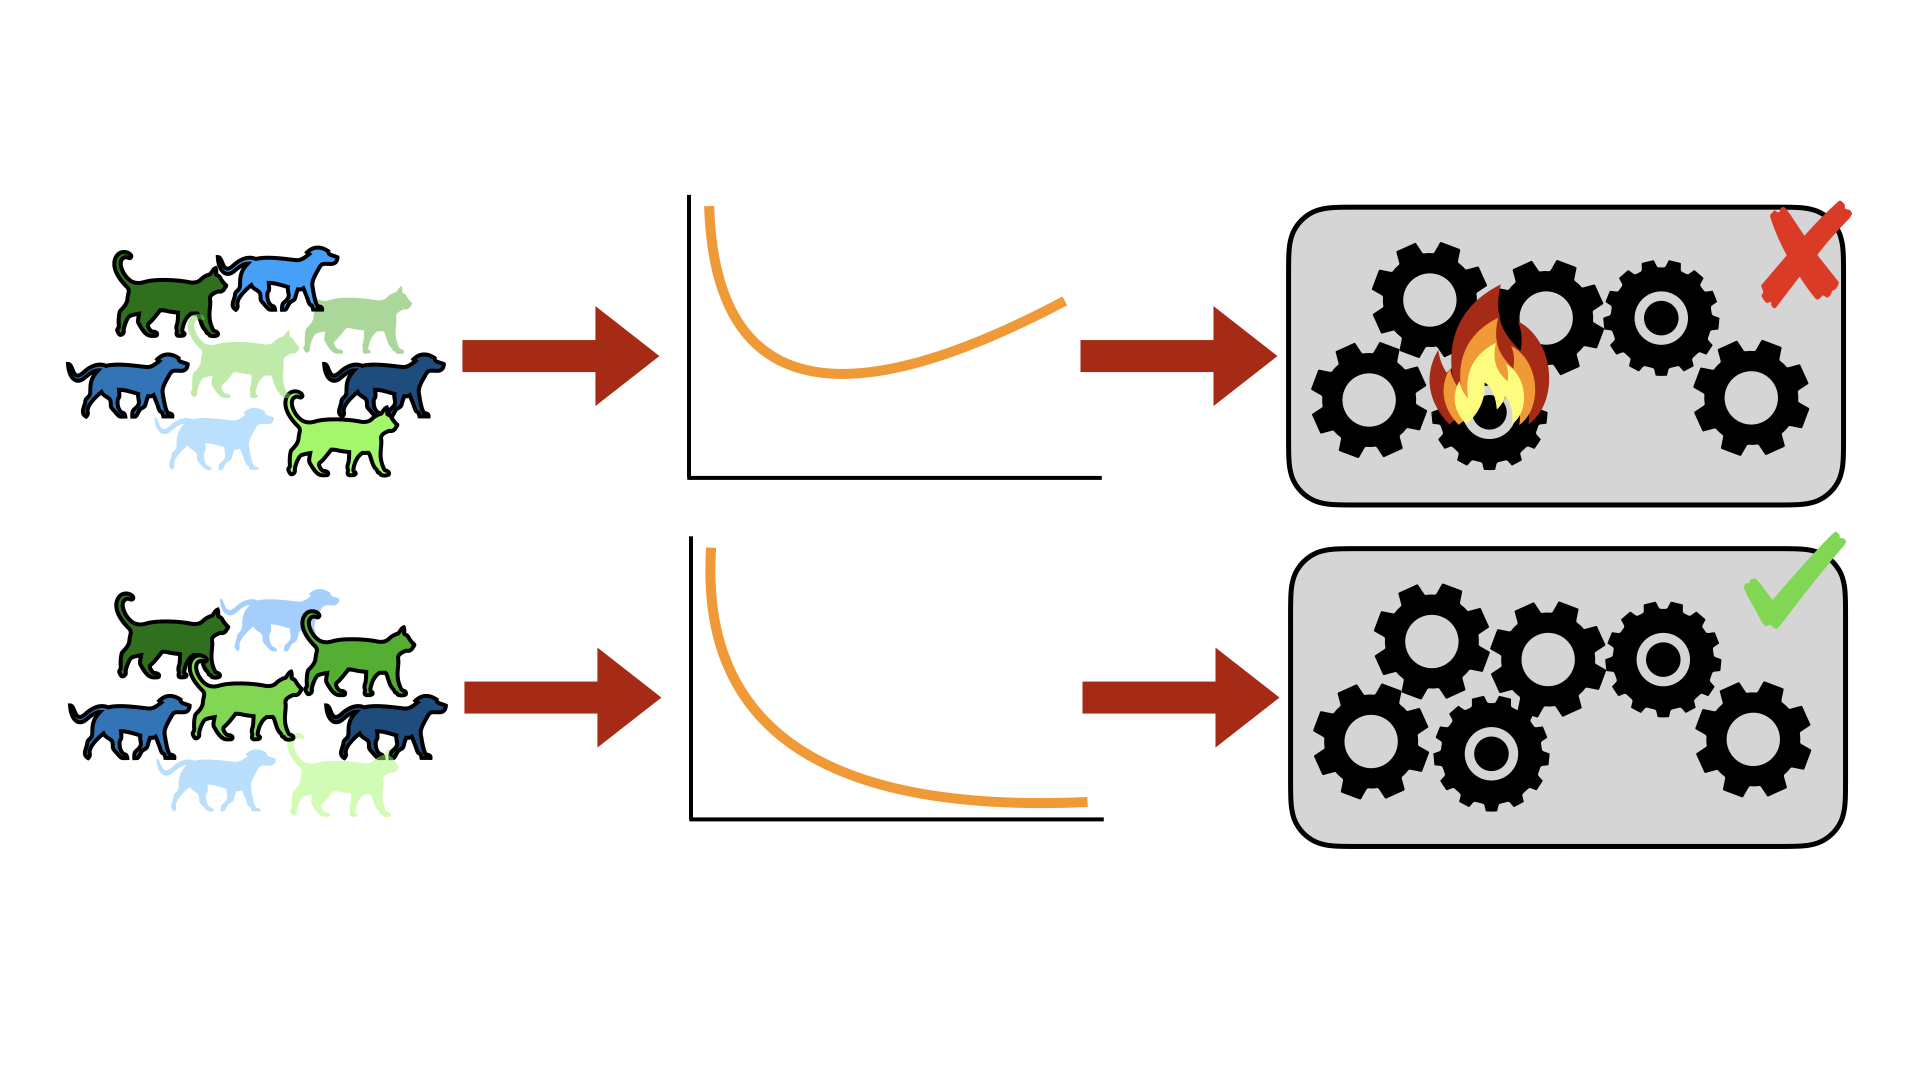
\includegraphics[trim={0 4.5cm 0 4cm},clip,width=0.9\textwidth]{diss/1_intro/figs/sample_select.png}
    \caption[Visualization of sample selection]{An example of identifying specific samples important to the learning task.}
    \label{fig:sample_select}
\end{figure}


\begin{mdframed}[style=MyFrame]
\textbf{ Thesis Goal: }
\em Identify, construct, and evaluate methods for \textbf{efficient} subset identification in modern machine learning feature, model, and input spaces.
\end{mdframed}

\section{A Few Motivating Examples}
Consider a traditional machine learning classification task in which we would like to predict whether an individual has a specific disease condition based on a medical resonance image (MRI) scan of their brain. Our input feature $x$ may consist of a 3D-array of values in $\RR^{\cI\times \cJ\times \cK}$ measuring some intensity of the imaging modality at each voxel, indexed by a tuple $(i,j,k) \in (\cI,\cJ,\cK)$.
Our outcome variable $y$ may simply be a binary label of whether the input scan has been labeled by a radiologist as one demonstrating typical disease characteristics.
Using an off the shelf 3D convolutional neural network with adjustments to match our input size, we can very quickly set up and train a system to predict disease presence with a high degree of accuracy.

\paragraph{Example 1.}
With a prediction for a specific scan, or predictions over a number of scans, we might be interested in identifying which regions of the brain are most important for diagnosis. These regions, $R \subset \cR:=\RR^{x\times y\times z}$, can be specific groups of pixels in the image that may correspond to known functional networks. Methods such as attention and class activation maps may work here, but there are a few issues. The number of samples available to learn a model is very small compared to the both the dimension of the input and the number of parameters in the model, i.e., $n \ll p$ and $n \ll d$. Thus it is very easy to overfit, and for areas of interest to be associated with intricacies of particular input data rather than true, real differences defined by the disease.

Furthermore, recent medical imaging studies have moved past simple difference detection: trends over time, and the ability to predict {\em future} disease development have by far become the setting of most interest.
Given an image of a healthy individual, is it possible to predict what their scan, or their future disease diagnosis, may be up to 10, 20, or more years in the future?
If a number of scans have been collected over some timeframe, can the \textit{trajectory} of the individuals' development be extrapolated to estimate progression?
As traditional models extended for temporal analysis grow in both size and complexity,
a number of subproblems explicitly related to model and input subspaces arise. In this thesis we address two such problems: \textbf{statistically rigorous identification of temporally evolving subsets}, and \textbf{characterizations of deep models that enable efficient training of recurrent models with large scale time-varying data}.
    
\paragraph{Example 2.}
With the rapid growth of AI and machine learning applications has come valid concerns regarding both guarantees of privacy.
Recent technology legislation has made the importance clear in all aspects of data use,
and particular projects and groups have demonstrated that machine learning is not independent of
this need \citep{Exposing}.
A new issue raised within this intersection is the ``right to be forgotten".
If a model has been trained with a particular users' data, 
they should have some recourse or right
to both remove their data from the training set,
and also know that the model has not learned from their data.
On the surface, this poses a significant problem for model builders
and organizations that spend large amounts
of time and resources in 
training deep learning models.

In the medical imaging example above this is especially important: with fewer samples it is more likely that information about any particular one could ``leak'', and the model's performance may degrade significantly as a relatively large percentage of it's training data is removed.
Thus tailored methods must be developed to ensure both privacy and performance, without requiring full retraining.
As we will see, 
\textbf{identification of model parameter subsets}
that are particularly important
for a particular sample's influence
in a model enables \textit{efficient machine unlearning}.

\paragraph{Example 3.}
From an alternative perspective, we may want to identify specific samples rather than have them specified a priori.
Traditionally a rigorous area of study under classical statistics, outlier detection and accounting have become a subfocus for many within the machine learning community as well \citep{golatkar2020eternal,golatkar2020forgetting,huang2020feature,ren2019likelihood}.
While subgroups of input samples may be outliers, it is more often the case that they represent known heterogeneity within the data. 
These differences may be marked using 
group information known a priori, and 
most learning tasks aim to learn tasks
in a \textit{subgroup-independent} manner.
In our disease prediction model above,
these groups could simply be stratified by the type of scanner used to acquire the image, but it could also
be a systematic difference correlated with some protected attribute. {\color{red} sentence about original brain atlas for registration being eurocentric}
This can directly lead to disparate performance and results on \textit{all} individuals outside of that group.
Optimization and regularization methods with this focus come under the umbrella of model fairness.
However, many existing methods do not scale well to larger models or as the number of subgroups grows, as is often the case when intersections of protected classes must be considered. Here we identify and construct a particular solution for \textbf{groupwise fairness that enables efficient in the loop fairness regularization}.

% What features are most important for prediction?
% Which samples were most important for my training?
% Can we understand when a model is certain or uncertain about its output?
% Are there layers in my network that have learned a particular subtask?
% Questions of robustness, bias, influence, fairness, and importance have become central questions to contemporary machine learning research \citep{doshi2017towards,mehrabi2021survey,amodei2016concrete}.
% machine learning, etc.

% Feature selection in the case of
% typical regression or classification 
% takes some form of learning parameters $\theta$ that allow for $\hat{y} = f_\theta(x)$ to be close to the true outcome of interest $y$.
% While forms of data $X := (x,y)$ may simply be continuous and real-valued, modern machine learning has greatly expanded formulations of the classical learning problem to include a wide variety of structured learning problems~\citep{nowozin2011structured}. 
% Consider the case when a high-dimensional input is used to predict an output with a highly-parametrized model. 
% Once learned, obvious questions arise as discussed above: are there specific low-dimensional spaces in either the input or the model space that are most important or necessary for the global learning problem of interest? Are there specific subspaces associated with particular subproblems of the global problem?
% The machine learning literature has come up with a number of ways to identify analogs of these spaces, 
% including extensions of sensitivity analysis to deep learning~\citep{yeung2010sensitivity,zhang2015sensitivity}, and constructing and identifying nonzero model subsets via particular model choices such as activations~\citep{selvaraju2017grad} and regularizers.
% In classical settings these are well understood: decision trees naturally provide ease of interpretibility via the information used to choose splits, and both linear and kernel support vector machines have been analyzed to provide for measures of sample importance via distances to the margin as well as feature importance via weights defining the learned hyperplane~\citep{Mitchell97}.
% Attention and saliency maps have emerged as popular new methods,
% given their ease of implementation and interpretation~\citep{sutskever2014sequence,vaswani2017attention,selvaraju2017grad}.
% By learning dimensions of a given input that are particularly important, either in a hard (binary) or soft (continuous weighting) manner, model builders are better able to understand and interpret what a model has learnt.
% The specific ideas of attention notwithstanding, many of these existing methods are far removed from traditional hypothesis testing frameworks.
% While some work has begun in this direction~\citep{tansey2018black},
% there remains a gap in direct identification of subsets and structures in these spaces that can be defined in statistically rigorous manners.

% \begin{figure}
%     \centering
%     \includegraphics[width=0.5\textwidth]{example-image-a}
%     \caption[A simple subset selection example]{\color{red} Identifying and selecting in MRIs, subset, sample, model ID.}
% \end{figure}

% \paragraph{A specific example.} 

% ------------------------------------------

% below here will be moved and arranged with the "selection" sections and here if relevant

% ------------------------------------------

% While attention can be directly applied to the network in order to identify ``hotspots" in the input space relating to the learned classification task, 
% given the high-dimensional nature of the input
% and the relatively small sample size 
% associated with medical imaging data, 
% it is very likely that an area of interest identified
% may be an intricacy of the training samples used rather than truly a region of disease signal.
% Class activation maps (CAMs) may be unclear, and can often associate with image artifacts unrelated to the scientific task~\citep{adebayo2018sanity}.
% Methods of generalization may help to increase confidence in identified regions, but statistical guarantees often remain out of reach.

% Furthermore, most recent problems associated with medical data have moved past simple difference detection: trends over time, and the ability to predict {\em future} disease development has by far become the setting of most interest.
% Given an image of a healthy individual, is it possible to predict what their scan, or their future disease diagnosis, may be up to 10, 20, or more years in the future?
% If a number of scans have been collected over some timeframe, can the \textit{trajectory} of the individuals' development be extrapolated to estimate progression?
% As traditional models extended for temporal analysis grow in both size and complexity,
% a number of subproblems explicitly related to model and input subspaces arise. Here we address two such problems: \textbf{statistically rigorous identification of temporally evolving subsets}, and \textbf{characterizations of deep models that enable efficient training of recurrent models with large scale time-varying data}.

% A sample's particular influence on model parameters aside, the identification of influential samples or subsets of samples more generally is of independent interest. 
% Traditionally a rigorous area of study under classical statistics, outlier detection and accounting have become a subfocus for many within the machine learning community as well \citep{golatkar2020eternal,golatkar2020forgetting,huang2020feature,ren2019likelihood}.
% While subgroups of input samples may be outliers, it is more often the case that they represent known heterogeneity within the data. 
% These differences are typically marked using 
% group information known a priori, and 
% most learning tasks aim to learn tasks
% in a \textit{subgroup-independent} manner.
% Optimization and regularization methods with this focus come under the umbrella of model fairness, and instead of identifying and boosting independences within the model or data, we aim to minimize them.
% However, many existing methods do not scale well as the number of subgroups grows, as is often the case when intersections of protected classes must be considered. In the sequel we identify and construct a particular solution for \textbf{groupwise fairness that enables efficient in the loop fairness regularization}.

\begin{mdframed}[style=MyFrame]
\em 
Here we focus our effort on identifying these important subsets of model, feature, and sample space for feature association, model size reduction, model unlearning, and, fairness. Specifically, taking advantage of both existing statistical and geometric methods, we develop new methods for localizing subsets in a range of settings from hypothesis testing to deep learning.
\end{mdframed}

\section{Thesis Scope and Contributions}

We explore the intersections of classical statistical and geometric constructions with modern machine learning methods. 
Figure~\ref{fig:scope} shows the overall scope projected along three axes: feature, parameter, and sample spaces.
Below we briefly introduce the main problems studied in this thesis.
\begin{figure}[!ht]
    \centering
    % \includegraphics[width=0.99\linewidth]{scope.pdf}
    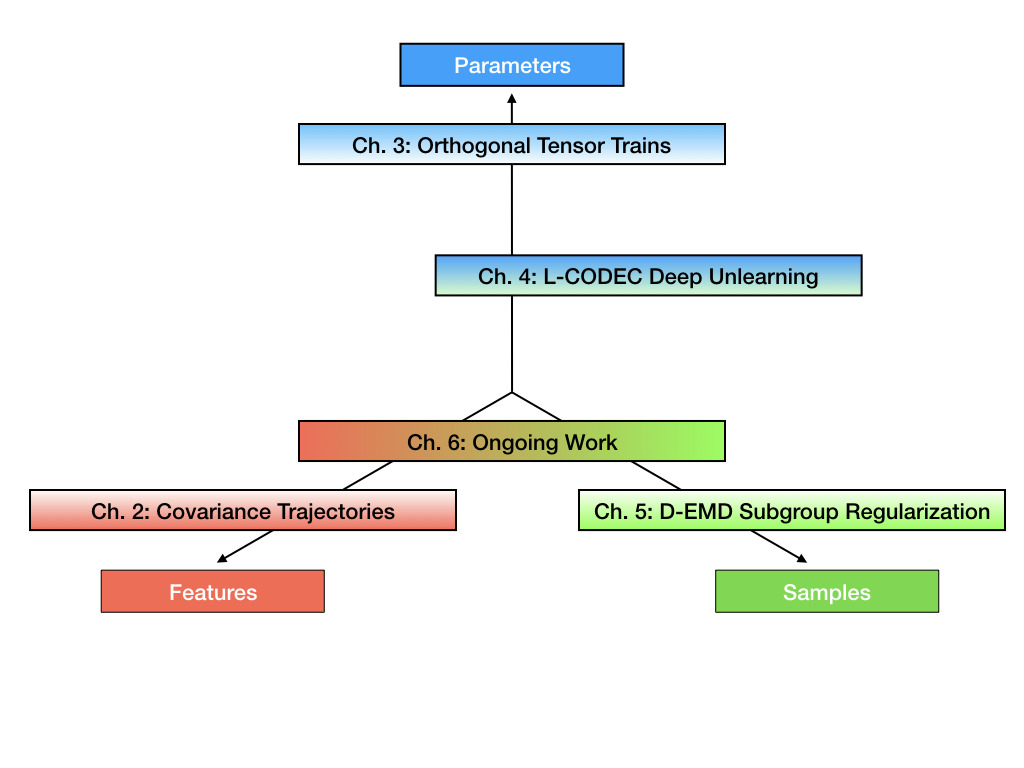
\includegraphics[width=0.95\linewidth]{diss/1_intro/figs/thesis_scope.png}
    \caption[Thesis Scope]{Thesis scope, projected over three representative axes. {\color{red} update chapter numbers shift by 1}}
    \label{fig:scope}
\end{figure}

\subsection{Second-Order Modeling and Group Difference Analysis over Time}

Recent results in coupled or temporal graphical models offer schemes for estimating the relationship structure 
between features when the data come from
related (but distinct) longitudinal sources. A novel application of these ideas is for analyzing group-level differences, i.e., in identifying if {\em trends} of estimated objects (e.g., 
covariance or precision matrices) are different across disparate conditions (e.g., gender or disease). Often, poor effect sizes make detecting the \textit{differential} signal 
over the {\em full} set of features difficult: for example, 
dependencies between only a {\em subset of features} may manifest differently across groups.
We first suggest
a parametric model 
for estimating trends in the space of $\SPD$ matrices as a function of one or more covariates.
We will then generalize scan statistics to graph structures, 
to search over distinct subsets of features (graph partitions) whose temporal dependency structure may show statistically 
significant group-wise differences.
We will theoretically analyze the Family Wise Error Rate (FWER) and bounds on Type 1 and Type 2 error. 
On a cohort of individuals with risk factors for Alzheimer's disease (but otherwise cognitively healthy), 
we 
find scientifically interesting 
group differences where the default analysis, 
i.e., models estimated on the full set of features, do not survive reasonable 
significance thresholds. 
% Preliminary work on this was published in \citep{covtraj}.


\subsection{Efficient Tensor Representations for Feasible Temporal Deep Learning}

Modern deep networks have proven to be very effective for analyzing real world images.
However, their application in medical imaging is still in its early stages,
primarily due to the large dimension of three-dimensional images, requiring enormous convolutional or fully connected layers --
if we treat an image (and not image patches) as a sample. 
These issues only compound when the focus moves towards longitudinal analysis
through recurrent structures, and when a point estimate of model parameters is insufficient 
in scientific applications where a reliability measure is necessary.
Using insights from differential geometry, 
we will adapt 
the tensor train decomposition to construct networks
with significantly fewer parameters,
allowing us to train powerful recurrent networks on whole brain image volumes. 
We analyze 
the \textit{orthogonal tensor train},
and demonstrate its ability to express a standard network layer both theoretically and empirically.
We 
demonstrate its ability to 
effectively reconstruct whole brain volumes
with faster convergence and stronger confidence intervals
compared to the standard tensor train decomposition. 
We provide code and show experiments on the ADNI dataset
using image sequences to regress on a cognition related outcome.
% Preliminary work on this was published in \citep{ott}.

\subsection{Practical Unlearning via Large-Scale Conditional Independence Testing}

%With AI systems extensively using personal %data for model training, 
Recent legislation has
led to interest in {\em machine unlearning}, i.e., removing specific training samples from a {\em predictive} model as if they never existed in the training dataset. 
Unlearning may also be required due to  corrupted/adversarial data or simply a user's updated privacy requirement.
For models which require no training ($k$-NN), 
simply deleting the closest original sample can be effective. 
%However, it is not clear how such approaches can be used to unlearn 
%models that contain rich information learned from the original data.
But this idea is inapplicable to models which learn richer 
representations.
%from data. 
%Recently, optimization-based unlearning estimators have been proposed, but 5their 
Recent ideas leveraging optimization-based updates
scale poorly with the model dimension $d$,  
due to 
inverting the Hessian of the loss function. %with an overall cost of $O(d^3)$ 
%is prohibitive.
We describe
a variant of a new conditional independence coefficient, 
L-CODEC, to identify a subset of the model parameters with the most semantic overlap on an individual sample level. 
Our approach completely avoids the need to invert a (possibly) huge matrix. 
By utilizing a Markov blanket selection, 
we find
that L-CODEC is also suitable for deep unlearning,
as well as other applications in vision.
Compared to alternatives, L-CODEC makes approximate unlearning possible 
in settings that would otherwise be infeasible, 
including vision models used for face recognition, 
person re-identification 
and NLP models that may require unlearning samples identified for exclusion.
% Preliminary work on this will appear in \citep{lcodec}.


\subsection{Reducing Subgroup Fairness via High Dimensional Earth Mover's Distances}

Optimal transport has recently emerged as a useful tool for machine learning through its connections with geometry, statistical machine learning, and through practical algorithms. Existing methods that leverage optimal transport often  regularize using  a Wasserstein metric or by computing barycenters, for example. %which are effective when distributions are continuous and known, or when measures of interest are discrete.
% Our formulation allows for a discretization of continuous measures that drop in directly to classical  formulations of the Earth Mover's Distance. 
We leverage optimal transport, except that we take advantage of a recently-introduced algorithm that computes a generalized earth mover's distance.
Not only is this algorithm computationally cheaper to compute compared to existing barycentric measures, but our method has the additional  advantage that gradients used for backpropagation can be directly read off of the forward pass computation, which leads to substantially faster model training.
We provide technical details about this new regularization term and its properties, 
and 
experimental demonstrations of improved training speed over existing Wasserstein-style methods.

{\color{red}
\subsection{Understanding Latent Spaces via Conditional Independences}

The final chapter of this thesis applies some of the tools developed above in the analysis of latent spaces in recent large scale models.
% In these studies, 
% we aim to identify conditionally independent features and subjects that are particularly important to the prediction and estimation of
% key disease outcomes,
% as a function of a number 
% of demographic, neuropsychological,
% genetic,
% and imaging data collected as 
% part of an ongoing consortium 
% to understand the progression
% of Alzheimer's disease in younger, 
% asymptomatic populations.
% In what follows we present
% exploratory analysis
% on a small, easily 
% digestible subset of the available data,
% that lays the foundation for
% further analysis.
}
% This work is the most forward looking, and aims to be a stepping stone toward a rigorous 

\section{Outline}
Chapter 2 covers the essential background necessary for the developments presented in the following chapters, including specifics of graphs and hypothesis testing, as well as relevant modern methods for learning and optimization.
In Chapters 3 through 7, we describe four perspectives to address subset identification.
Chapter 3 explores and focuses on the identification of feature subsets varying over time.
In Chapter 4 we describe a method of constraining the parameter space in a particular manner
that enables more efficient large scale neural networks.
Next, Chapter 5 provides a solution to the machine unlearning problem,
enabled through a particular conditional independence parameter selection scheme, vastly reducing network update costs.
Chapter 6 ends with a unique solution to subgroup fairness, 
where we take advantage of an efficient solution to
the $d$-dimensional earth mover's problem
to regularize large models when the number of subgroups can be large.
{\color{red} Chapter 7 describes future work, focused on applying a particular solution from Chapter 5 to understanding relationships among features in latent spaces learned by large generative models.}


%%%%%%%%%%%%% 
% Some old stuff

% Significant progress in the modern development of machine learning has
% been built upon connections and patterns identified across myriad
% interdisciplinary fields of study.
% Up through the mid 2000's, 
% many of these methods were inspired by and interested in 
% highly focused and constrained problems. 
% With a reasonably sized input domain, could a model of roughly equal size be used to
% predict some output?
% Linear regressors, decision trees, and support vector machines were all answers to these questions, with their own
% varying degrees of scaling and complexity.
% These methods necessitated carefully constructed formulations with specific restrictions to the learnable function class,
% enabling straightforward analysis 
% for provable performance guarantees 
% and easy identification of critical training samples and important input features.

% Contemporary machine learning, however, has a vastly different modus operandi. 
% Driven in large part by the exponential growth of available computation via Moore's Law, \textit{deep learning} has fallen squarely in the realm of \textbf{over-parameterized} models.
% With these overparametrizations and computation capacity, the typical learning questions posed as maximizing accuracy or reducing error have largely been addressed for even large scale problems.
% As such, complementary questions have led to subfields focusing on other performance measures, such as robustness, fairness, interpretability, and explainability.
% Many solutions to these questions end up looking back at answers found for the under- or non-parametrized settings.
% While nascent, these approaches 
% attempt to fill the gap between
% statistical and deep models to enable similar measures of sample influence, feature importance, and model analysis. 
% Most notable amongst these newer approaches is that of (Self)-Attention in Neural Networks \citep{sutskever2014sequence,vaswani2017attention}.
% Other proposals 
% end up looking back at the types of analysis typical of those more classical under-parametrized or nonparametrized methods.

% Not limited to previous developments in learning or computation theory, the arguably most valuable contributions toward the exponential reduction in model error can be attributed to influences and intuitions taken
% from biology, psychology, neuroscience, and even XXX \citep{srivastava, etc}.
% Perhaps one explanation as to why this phenomenon exists may be attributed to the way in which deep learning evolved. 
% The classical learning goal of function approximation lends itself nicely to a system which allows for arbitrary complexity via simple changes (e.g., addition of neural network layers). % Foundational works building on the original neural networks particularly have taken advantage of constraining this space of functions to search over: 
% the most seminal case being those of convolutional filters for imaging data. 
% While ``constraints" of this form have helped tremendously in model performance on modern vision and language machine learning tasks (GANs, Recurrent Networks, Residual Layers, Transformers, etc.), the ability to identify \textit{subsets} of important samples, input features, and model parameters has lagged significantly behind the development of these methods.
% Recently larger interest has been taken by the community to understand and interpret models with this view, only after extremely large and opaque models have become ubiquitous.
%This lag directly explains the more recent interest in developing methods for understanding and interpreting large scale machine learning models.
% \chapter{Introduction} \label{chap:intro} 

Modern applications of machine learning in a broad range of industrial and consumer-facing systems have become ubiquitous.
Most interactions with daily technologies now intrinsically involve 
a request to some ``smart`` system in the ``cloud'', 
where those interactions range from
a request for map directions 
to simply loading a webpage.
Neural network models, and the recent advances of deep learning,
have enabled these systems that 
make such applications possible.
These models have achieved
human-level performance on learning tasks
including image classification~\citep{resnet,alexnet}, image segmentation~\citep{segmentation}, video analysis~\citep{zhang2016video}, text understanding and generation~\citep{bert,gpt}, and have slowly begun to solve more fundamental scientific problems such as protein folding~\citep{protein} drug discovery~\citep{drugdisc}, and medical diagnosis~\citep{diag}.
While this performance is largely attributed to model size,
the abundance of high quality training data
has equally contributed to real world performance,
enabling model training over millions of real world samples~\citep{imagenet,laion},
and potentially billions of synthetic samples via environment simulation~\citep{mcts}.

While deployment in some domains (recommender systems, object detection) may benefit almost unconditionally from this vastly expanded capability, rightful hesitancy has limited their widespread use in particular applications where impacts on individuals, people, or environments may be at stake.
These ``last mile'' concerns take a few forms.
% Because a completely accurate model is still out of reach, an important question that needs to be answered is: which inputs or individuals are being given incorrect outcomes, and why?
% maybe a sentence suggesting unlearning/removal
In mission critical applications such as medical diagnosis, 
the impact of an error can be extremely large,
even if a misprediction happens extremely infrequently.
Additionally, large scale model training and architecture search
can require exorbitant amounts of energy producing high emissions,
and their scale can limit market participants
to only large actors with vast existing resources.
The accessibility and effectiveness of these models can also vary significantly based on the training data, and disparate outcomes can be exacerbated by existing social inequity.

While existing human or ``natural'' systems that these models aim to assist are not perfect, 
our real world has developed norms and regulations that 
enable them to function.
A medical diagnosis might require a physician to explain what symptoms led them to that particular conclusion.
Energy metering and carbon taxes may be applied to limit
emissions.
Regulatory satisfaction may require 
analysis proving equal opportunity,
or that specific protected classes
are not used in decision making.
% Specifically, these can include ideas as simple as the Hippocratic Oath and medical malpractice insurance, to asking your doctor what symptoms lead them to a particular diagnosis.
These ideas are difficult to directly translate to automated machine learning systems,
but proxies have been identified that we can build upon.

These norms and regulations answer a number of questions we may also try to pose to our machine learning models.
What is the cost to learn this task?
What led to this particular outcome?
Why is this outcome different from another?
% We will explore how these questions can be formulated concretely. 

If the answer to these questions is negative or unknown,  follow-up questions all take an interesting form:
Can we learn a smaller model with similar performance? 
Can we identify the most important features? 
Which individuals or groups are being treated unfairly, and can we change that?
These questions ask us to identify a \textit{subset} of some relevant set, dependent on setting, and this identification is our focus here.

% Moving specifically to machine learning methods,
Taking a step back, let's take a look at a representative system. Figure~\ref{fig:dl} illustrates a typical learning pipeline. 
A dataset is collected and used to train a model, by minimizing the error over
those samples in the dataset (top).
A ``sample'' can be a single measured value, or it can
be a large, highly structured object with many ``features.''
The model is made up of some ``parameters'' that are 
tuned during training to learn a good predictor over the training dataset.
This model is then used to predict, or \textit{infer}, on new
data seen ``in the wild'' (bottom).
Our questions above are formally asking to identify \textit{subsets of these objects}: is a subset of the model parameters sufficient for learning? Which subset of the features are important for a prediction? Which subset of the dataset exhibit a specific attribute?
\begin{figure}
    \centering
    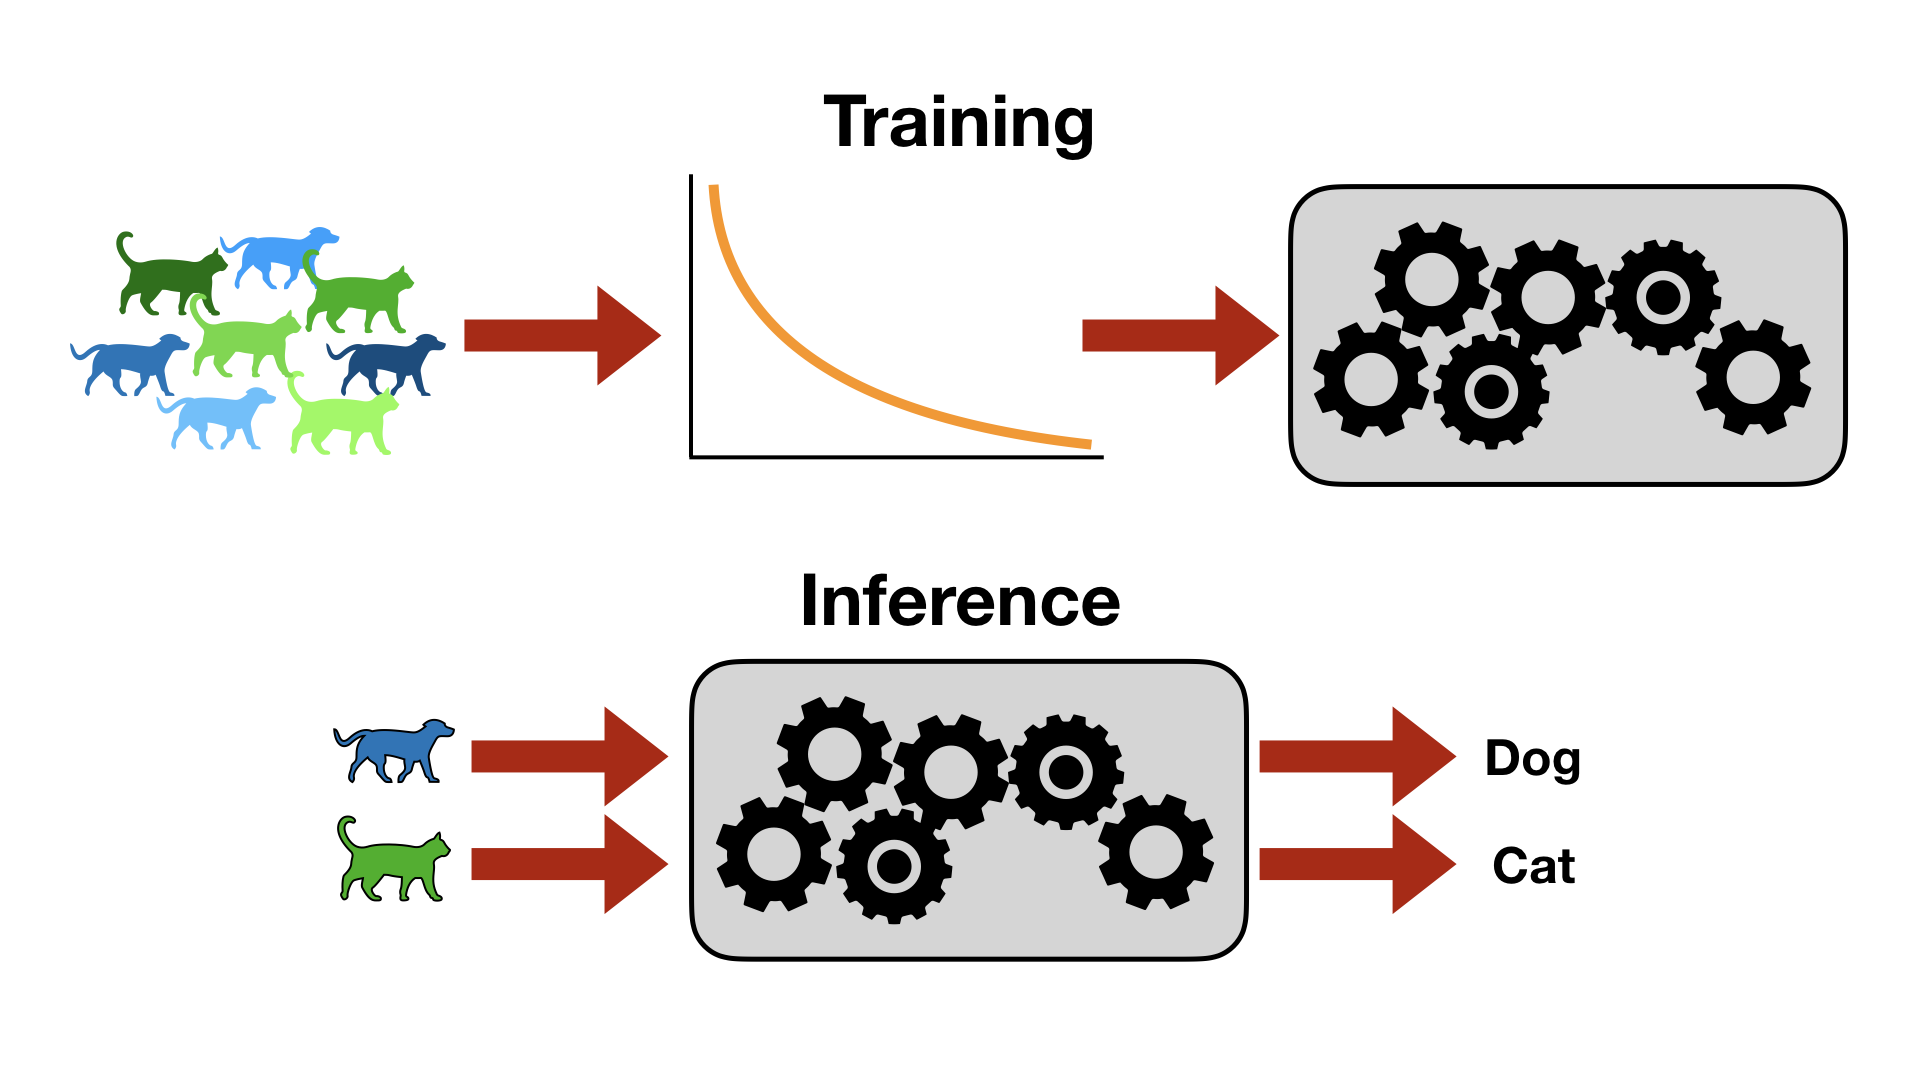
\includegraphics[trim={0 3cm 0 3cm},clip,width=0.95\textwidth]{diss/1_intro/figs/dl.png}
    \caption[Modern machine learning pipelines]{Machine learning training and inference visualization.}
    \label{fig:dl}
\end{figure}

% \textit{Explainability} can be seen as identifying important features of the input, as well as parts of the model (parameters) that ``light up`` for that input. \textit{Fairness} can be evaluated via measures over subsets of the data that correspond to specific groups. 

\begin{mdframed}[style=MyFrame]
\em 
\textbf{This thesis} focuses its main efforts on identifying these important subsets of model, feature, and sample space, to enable answering questions necessary for mainstream adoption of machine learning methods.
\end{mdframed}

% In this dissertation, we explore the sizes of these models, samples, and datasets, and 
% analyze under what situations 
% a smaller \textit{subset} of them may be sufficient or important
% for questions that run parallel to standard performance and accuracy measures.

Let us step a bit deeper into a basic illustrative example. In order to ease understanding, we can first begin with a basic formulation of learning methods, from which the questions above can take specific forms. 
Learning methods typically  try to identify a function mapping (model) that is able to complete a specific task at some high level of profficiency.
% In Figure~\ref{fig:dl}, a model is trained using examples of classification task (top), in order to accurately predict the class of a newly provided input (bottom).
% \begin{figure}
%     \centering
%     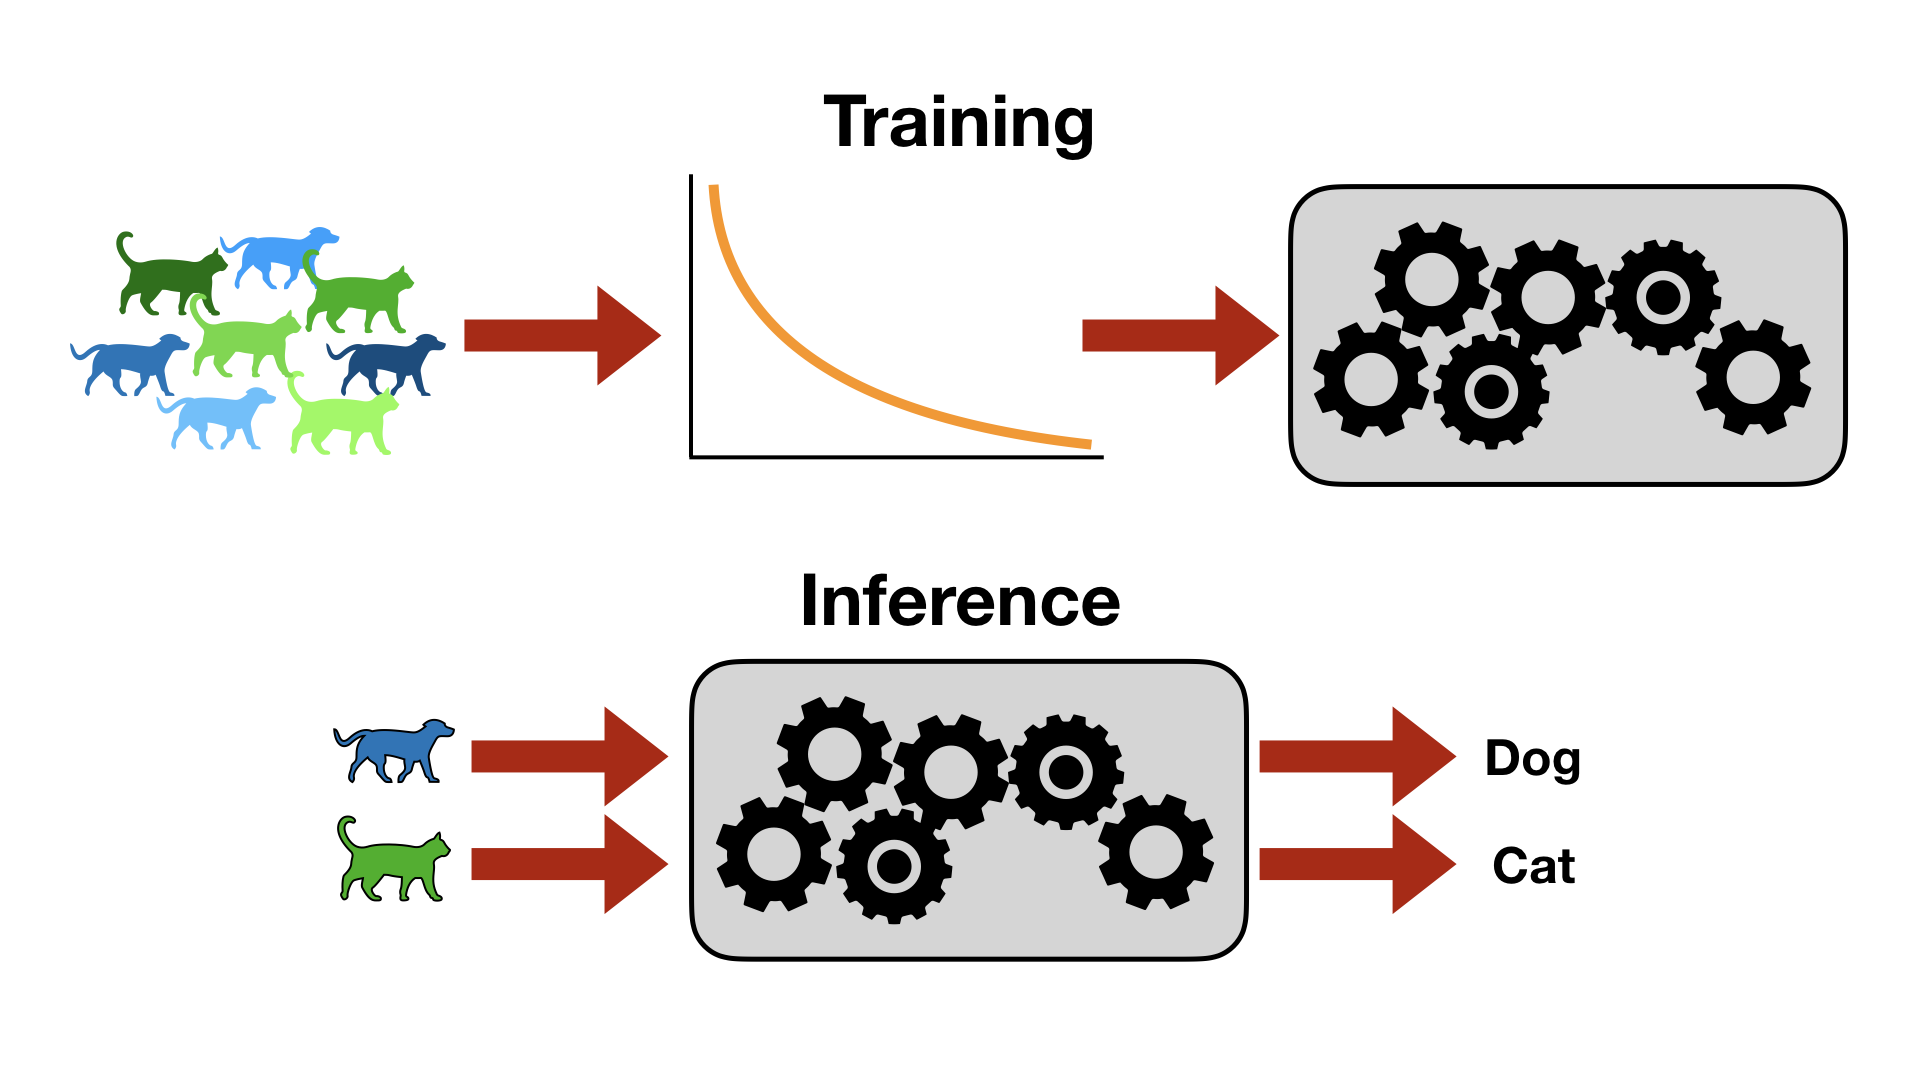
\includegraphics[trim={0 3cm 0 3cm},clip,width=0.95\textwidth]{diss/1_intro/figs/dl.png}
%     \caption[Modern machine learning pipelines]{Machine learning training and inference visualization.}
%     \label{fig:dl}
% \end{figure}
Say we have some dataset comprising of sample pairs $(x,y)$, where we wish to predict $y$ from $x$.
Our prediction, say $\hat{y}$, might be the output of some unknown function $f$ that we attempt to learn from training data. 
Let our approximation to this function be $\hat{y}:=\hat{f}(x)$.
This can take many forms, 
based on assumptions and prior information we may have on the relationships among the data. 
Consider the simple \textit{linear} case,
where we want to learn some parameter $w$ such that $y = w\cdot x$. 
Given $n$ sample pairs $(x_i,y_i)$ indexed by $i$, traditional statistics and optimization literature yield the following \textit{least squares} problem formulation, where we want to minimize the ``squared error'' between the observed values $y_i$ and the predicted $\hat{y}_i:= w\cdot x_i$:
\begin{align}\label{eq:lq}
\hat{f}:=\hat{w} = \mathop{\arg\min}_{w} \sum_{i=1}^n (y_i - w\cdot x_i)^2
\end{align}
This formulation expands without much change to a multi-dimensional form of the input $x$ and respectively, $w$: the canonical case where a number of features, or \textit{covariates} (e.g., symptoms), are used together to predict the outcome (e.g., diagnosis). 
If we are interested in which features of $x$ are important, we can look at the relative values of the learned ``weights'' $w$. In this simple setting, the importance of a feature (say $x^j$) can be exactly determined by the importance of the parameter ($w^j$).
A weight value far from zero may indicate that corresponding feature is important for diagnosis.
% If instead we are interested in which samples are most important, we can use existing methods for sample reweighting or methods that use standard assumptions to efficiently identify important subsets.

In this case and others, traditional statistical learning methods 
have been studied 
for many decades.
Linear regressors, decision trees, and support vector machines
have all been analyzed under these lenses.
% ,
% and as the modern machine learning community
% has returned to these questions recently,
% so has a renewed interest in their methods of analysis.
New research focuses
particularly on the differences
associated with moving from classical \textit{under-parametrized} models to
modern (deep) \textbf{over-parameterized} models: where
the model size vastly outnumbers the number
of input samples.
% , and may even be comparable to 
% the \textit{entire sample space.}
Methods for estimating the number of samples needed,
the time to learn a particular task,
and the generalization ability 
all require new perspectives in this regime.
While nascent, this research
attempts to fill the gap between
statistical and deep models to enable similar measures of sample influence, feature importance, and model understanding. 

\paragraph{A full picture.}
Let us expand our notation from the example above to consider this more general framing.
Consider a dataset $X:=\{x_i\}_{i=1}^n$ of size $n$ where each data point $x_i$ in the set $X$ is drawn from some underlying distribution over the domain $x_i \sim \cX^d$, 
with domain dimensionality (number of features) $d$.
A model $f$ is fit using a parametrization $\theta \in \Theta$,
with $\Theta$ the space of possible parametrizations (models) with some intrinsic dimension $p$. 
%While all three of these problems are closely related, they require different approaches. 
Generalizing the least squares``error measure'' from Eq.~\eqref{eq:lq} to an arbitrary \textit{loss} $\ell$, we have
\begin{align}\label{eq:learning}
    \hat{f}:=\hat{\theta} = \mathop{\arg\min}_{\theta\in\Theta} \sum_{x \in X} \ell(f_\theta(x_i))
\end{align}
From an analysis perspective, 
we might be interested in any one of 
(a) subsets of input features $\cC \subseteq \cX$ that are important for the downstream task,
(b) associating model subsets $\cP \subseteq \Theta$ with specific inputs or groups of inputs, or 
(c) subsets or subgroups of samples $S \subseteq \{X\}$ that are sufficient or representative of the entire dataset.

Crucially, an uninformed search for a subset is computationally infeasible. For a superset of size $n=|X|$, The set of all subsets is the power set, with a size of $2^{n}$! If an identification procedure requires looking over all of these and choosing a ``best'' one by some metric, the procedure will be limited to very small supersets.
Efficient methods have been developed in each of the three contexts above to avoid this exponential search.

\begin{figure}
    \centering
    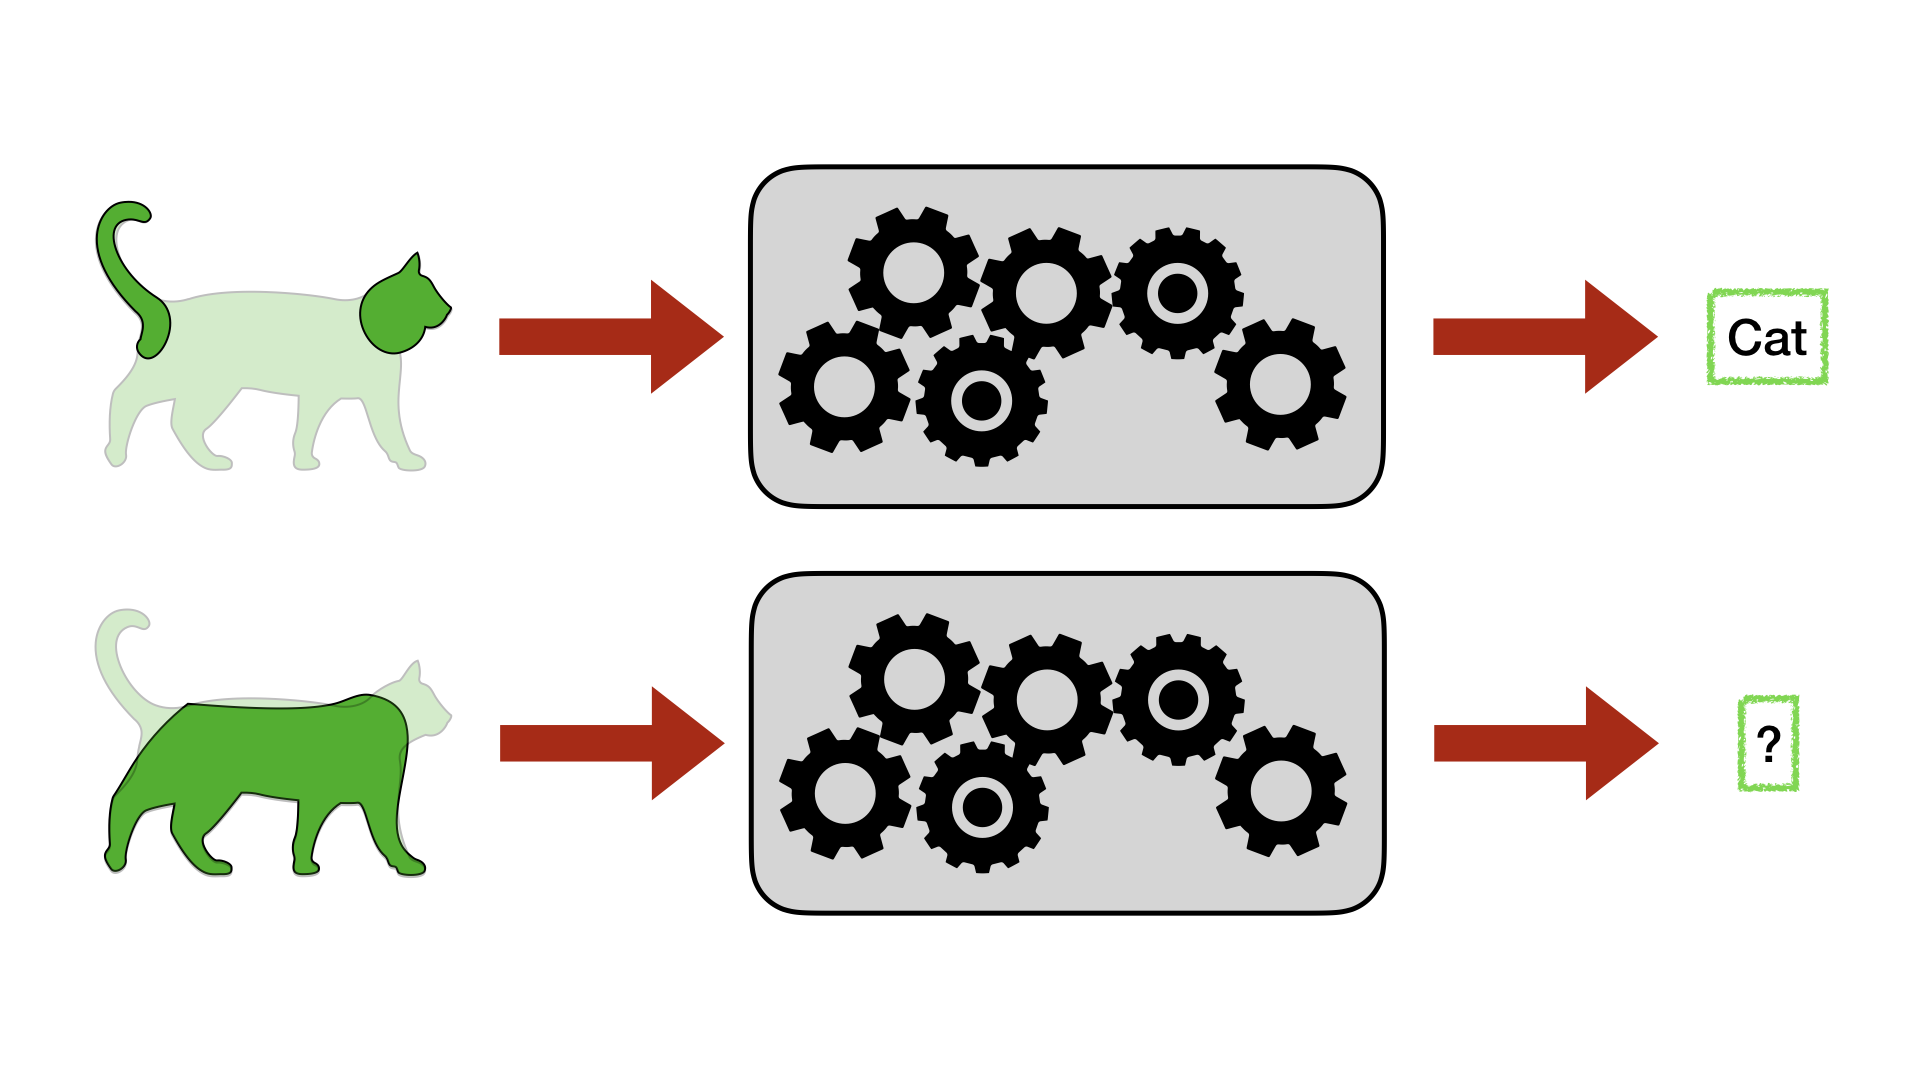
\includegraphics[trim={0 3cm 0 3cm},clip,width=0.9\textwidth]{diss/1_intro/figs/feat_select.png}
    \caption[Visualization of feature selection]{An example of identifying specific features important to the learning task.}
    \label{fig:feat_select}
\end{figure}
\paragraph{Feature Selection.} 
With more complex models $f$ compared to the linear case above, newer ``black-box'' methods have been developed for identifying important features. From the more pure statistics side, scan statistics~\citep{scanstat,scanstatlrt} allow for a structured ``scanning'' over the input space, skipping subsets unlikely to provide additional information for the measure of interest.
Further on the deep learning side, adaptations of sensitivity analysis, via noise addition and perturbations have found success~\citep{yeung2010sensitivity,zhang2015sensitivity}, alongside activation mapping~\citep{cam,selvaraju2017grad}.
These methods typically generate an analagous ``weighting'' over the input space, identifying features most salient for the specific task (Figure~\ref{fig:feat_select}).

\begin{figure}
    \centering
    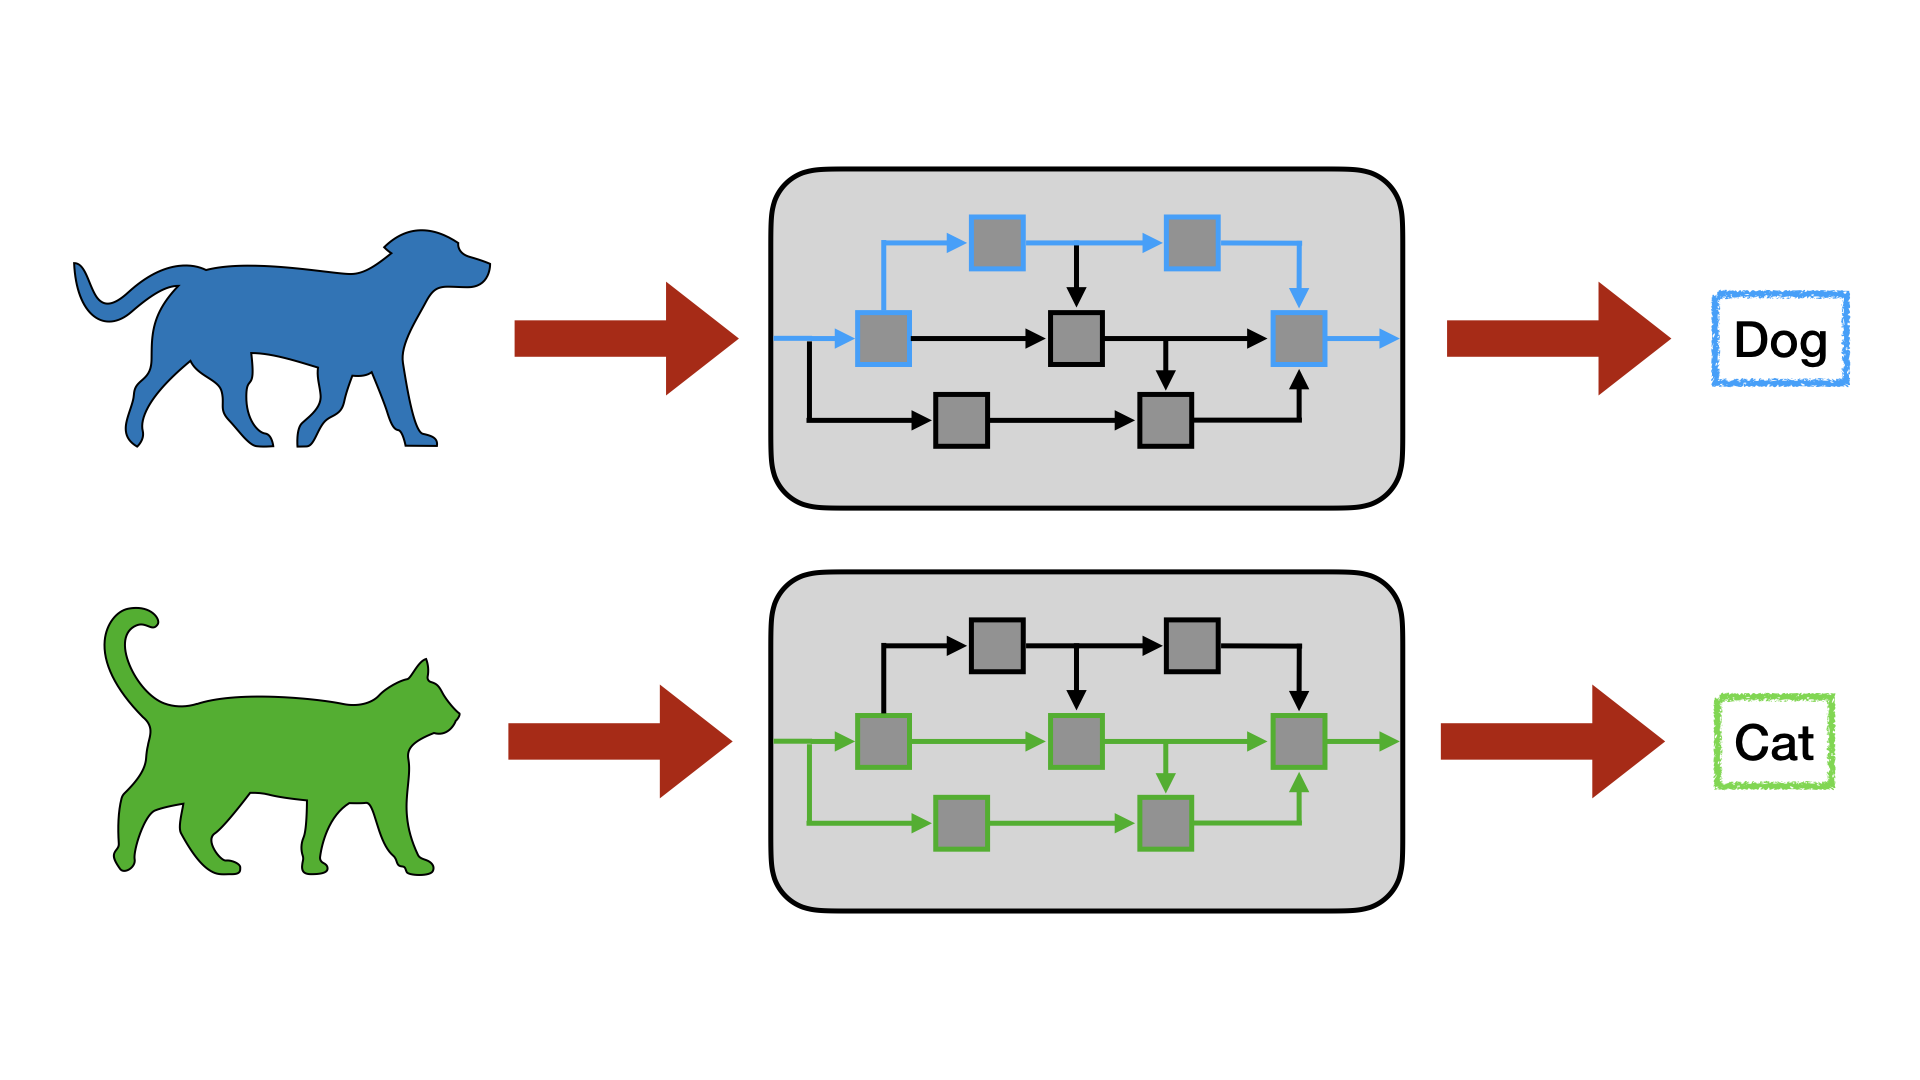
\includegraphics[trim={0 3cm 0 3cm},clip,width=0.9\textwidth]{diss/1_intro/figs/param_select.png}
    \caption[Visualization of parameter selection]{An example of identifying specific parameters important to the learning task.}
    \label{fig:param_select}
\end{figure}
\paragraph{Parameter Selection.} 
Selection in the model space generally takes two forms. First, as a prior, restriction, or assumption over the model space, and second, as a post-hoc method for an ``explainable'' proxy.
Regularization, sparsity, and gating methods are often used independent of the type or size of the model, to encourage the solution to fall within a specific region of the model space.
% In non-deep settings these methods come with strong theoretical guarantees. 
The theoretical underpinnings of these methods in deep learning are still being actively researched~\citep{hardt2016train,jacot2018neural,neyshabur2014search}, but the methods have nonetheless been effective in practice. 
On the post-hoc side, of particular interest are the parameters relevant to specific regions of the input space \textit{after} training (Figure~\ref{fig:param_select}). Here, recent analysis of deployed networks has shown this to be true~\citep{bau2017network,fong2018net2vec}, and current work continues to explore these network regions to aid in interpretability and explainability.

\paragraph{Sample Selection.} Many methods have been developed for outlier detection within training or testing sets~\citep{huang2020feature,ren2019likelihood} \textit{after} training, as well as methods for understanding sample influence~\citep{koh2017understanding,golatkar2020eternal,huang2020feature} . ``In-the-loop'' methods for accounting for ``outlierness'' behave similarly to accounting for group or individual fairness while training~\cite{mehrabi2021survey}. Unfortunately, once samples are identified in some manner, post-hoc adjustments to a trained model are generally very difficult. Recent work has focused on ``unlearning'', or removing a sample's influence on a model without retraining. If specific samples can be uniquely identified, performance and privacy reasons may require these specific interventions to reduce the ``influence'' of that sample subset.
\begin{figure}
    \centering
    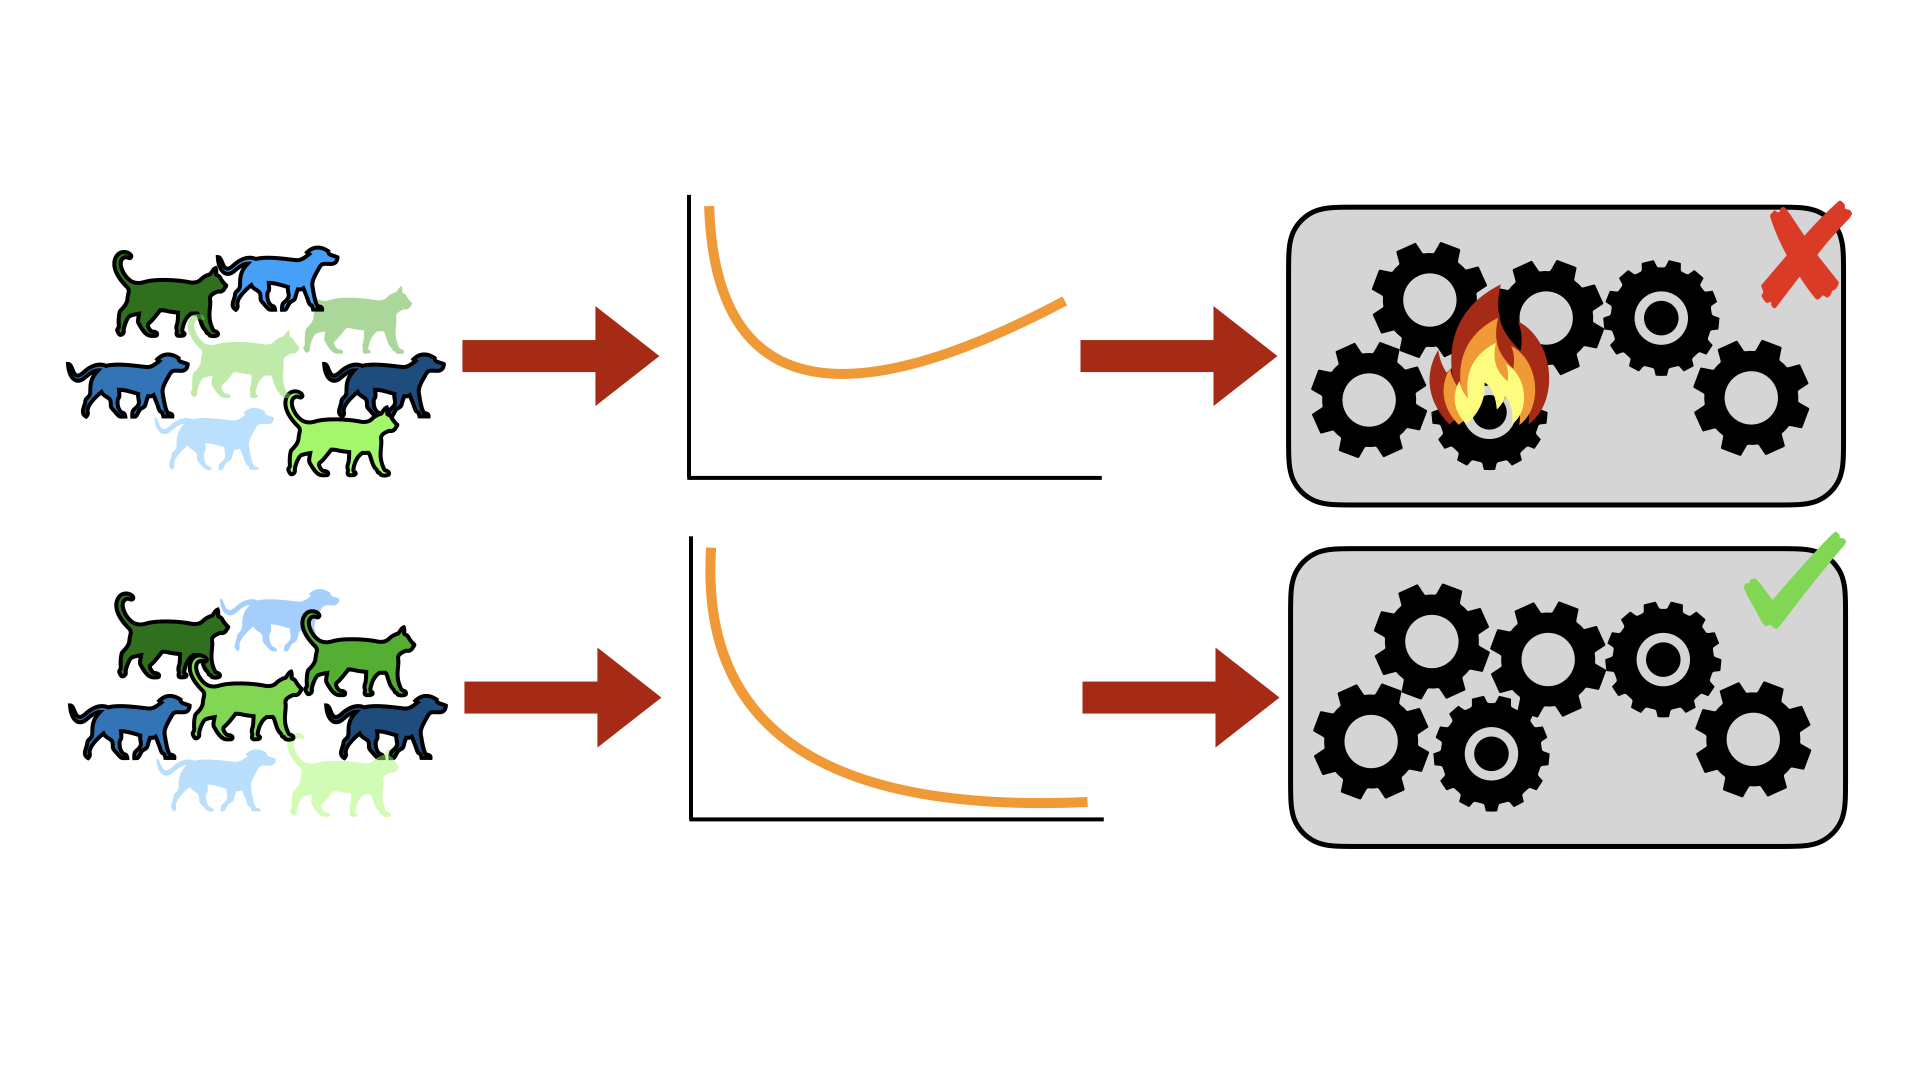
\includegraphics[trim={0 4.5cm 0 4cm},clip,width=0.9\textwidth]{diss/1_intro/figs/sample_select.png}
    \caption[Visualization of sample selection]{An example of identifying specific samples important to the learning task.}
    \label{fig:sample_select}
\end{figure}


\begin{mdframed}[style=MyFrame]
\textbf{ Thesis Goal: }
\em Identify, construct, and evaluate methods for \textbf{efficient} subset identification in modern machine learning feature, model, and input spaces.
\end{mdframed}

\section{A Few Motivating Examples}
Consider a traditional machine learning classification task in which we would like to predict whether an individual has a specific disease condition based on a medical resonance image (MRI) scan of their brain. Our input feature $x$ may consist of a 3D-array of values in $\RR^{\cI\times \cJ\times \cK}$ measuring some intensity of the imaging modality at each voxel, indexed by a tuple $(i,j,k) \in (\cI,\cJ,\cK)$.
Our outcome variable $y$ may simply be a binary label of whether the input scan has been labeled by a radiologist as one demonstrating typical disease characteristics.
Using an off the shelf 3D convolutional neural network with adjustments to match our input size, we can very quickly set up and train a system to predict disease presence with a high degree of accuracy.

\paragraph{Example 1.}
With a prediction for a specific scan, or predictions over a number of scans, we might be interested in identifying which regions of the brain are most important for diagnosis. These regions, $R \subset \cR:=\RR^{x\times y\times z}$, can be specific groups of pixels in the image that may correspond to known functional networks. Methods such as attention and class activation maps may work here, but there are a few issues. The number of samples available to learn a model is very small compared to the both the dimension of the input and the number of parameters in the model, i.e., $n \ll p$ and $n \ll d$. Thus it is very easy to overfit, and for areas of interest to be associated with intricacies of particular input data rather than true, real differences defined by the disease.

Furthermore, recent medical imaging studies have moved past simple difference detection: trends over time, and the ability to predict {\em future} disease development have by far become the setting of most interest.
Given an image of a healthy individual, is it possible to predict what their scan, or their future disease diagnosis, may be up to 10, 20, or more years in the future?
If a number of scans have been collected over some timeframe, can the \textit{trajectory} of the individuals' development be extrapolated to estimate progression?
As traditional models extended for temporal analysis grow in both size and complexity,
a number of subproblems explicitly related to model and input subspaces arise. In this thesis we address two such problems: \textbf{statistically rigorous identification of temporally evolving subsets}, and \textbf{characterizations of deep models that enable efficient training of recurrent models with large scale time-varying data}.
    
\paragraph{Example 2.}
With the rapid growth of AI and machine learning applications has come valid concerns regarding both guarantees of privacy.
Recent technology legislation has made the importance clear in all aspects of data use,
and particular projects and groups have demonstrated that machine learning is not independent of
this need \citep{Exposing}.
A new issue raised within this intersection is the ``right to be forgotten".
If a model has been trained with a particular users' data, 
they should have some recourse or right
to both remove their data from the training set,
and also know that the model has not learned from their data.
On the surface, this poses a significant problem for model builders
and organizations that spend large amounts
of time and resources in 
training deep learning models.

In the medical imaging example above this is especially important: with fewer samples it is more likely that information about any particular one could ``leak'', and the model's performance may degrade significantly as a relatively large percentage of it's training data is removed.
Thus tailored methods must be developed to ensure both privacy and performance, without requiring full retraining.
As we will see, 
\textbf{identification of model parameter subsets}
that are particularly important
for a particular sample's influence
in a model enables \textit{efficient machine unlearning}.

\paragraph{Example 3.}
From an alternative perspective, we may want to identify specific samples rather than have them specified a priori.
Traditionally a rigorous area of study under classical statistics, outlier detection and accounting have become a subfocus for many within the machine learning community as well \citep{golatkar2020eternal,golatkar2020forgetting,huang2020feature,ren2019likelihood}.
While subgroups of input samples may be outliers, it is more often the case that they represent known heterogeneity within the data. 
These differences may be marked using 
group information known a priori, and 
most learning tasks aim to learn tasks
in a \textit{subgroup-independent} manner.
In our disease prediction model above,
these groups could simply be stratified by the type of scanner used to acquire the image, but it could also
be a systematic difference correlated with some protected attribute. {\color{red} sentence about original brain atlas for registration being eurocentric}
This can directly lead to disparate performance and results on \textit{all} individuals outside of that group.
Optimization and regularization methods with this focus come under the umbrella of model fairness.
However, many existing methods do not scale well to larger models or as the number of subgroups grows, as is often the case when intersections of protected classes must be considered. Here we identify and construct a particular solution for \textbf{groupwise fairness that enables efficient in the loop fairness regularization}.

% What features are most important for prediction?
% Which samples were most important for my training?
% Can we understand when a model is certain or uncertain about its output?
% Are there layers in my network that have learned a particular subtask?
% Questions of robustness, bias, influence, fairness, and importance have become central questions to contemporary machine learning research \citep{doshi2017towards,mehrabi2021survey,amodei2016concrete}.
% machine learning, etc.

% Feature selection in the case of
% typical regression or classification 
% takes some form of learning parameters $\theta$ that allow for $\hat{y} = f_\theta(x)$ to be close to the true outcome of interest $y$.
% While forms of data $X := (x,y)$ may simply be continuous and real-valued, modern machine learning has greatly expanded formulations of the classical learning problem to include a wide variety of structured learning problems~\citep{nowozin2011structured}. 
% Consider the case when a high-dimensional input is used to predict an output with a highly-parametrized model. 
% Once learned, obvious questions arise as discussed above: are there specific low-dimensional spaces in either the input or the model space that are most important or necessary for the global learning problem of interest? Are there specific subspaces associated with particular subproblems of the global problem?
% The machine learning literature has come up with a number of ways to identify analogs of these spaces, 
% including extensions of sensitivity analysis to deep learning~\citep{yeung2010sensitivity,zhang2015sensitivity}, and constructing and identifying nonzero model subsets via particular model choices such as activations~\citep{selvaraju2017grad} and regularizers.
% In classical settings these are well understood: decision trees naturally provide ease of interpretibility via the information used to choose splits, and both linear and kernel support vector machines have been analyzed to provide for measures of sample importance via distances to the margin as well as feature importance via weights defining the learned hyperplane~\citep{Mitchell97}.
% Attention and saliency maps have emerged as popular new methods,
% given their ease of implementation and interpretation~\citep{sutskever2014sequence,vaswani2017attention,selvaraju2017grad}.
% By learning dimensions of a given input that are particularly important, either in a hard (binary) or soft (continuous weighting) manner, model builders are better able to understand and interpret what a model has learnt.
% The specific ideas of attention notwithstanding, many of these existing methods are far removed from traditional hypothesis testing frameworks.
% While some work has begun in this direction~\citep{tansey2018black},
% there remains a gap in direct identification of subsets and structures in these spaces that can be defined in statistically rigorous manners.

% \begin{figure}
%     \centering
%     \includegraphics[width=0.5\textwidth]{example-image-a}
%     \caption[A simple subset selection example]{\color{red} Identifying and selecting in MRIs, subset, sample, model ID.}
% \end{figure}

% \paragraph{A specific example.} 

% ------------------------------------------

% below here will be moved and arranged with the "selection" sections and here if relevant

% ------------------------------------------

% While attention can be directly applied to the network in order to identify ``hotspots" in the input space relating to the learned classification task, 
% given the high-dimensional nature of the input
% and the relatively small sample size 
% associated with medical imaging data, 
% it is very likely that an area of interest identified
% may be an intricacy of the training samples used rather than truly a region of disease signal.
% Class activation maps (CAMs) may be unclear, and can often associate with image artifacts unrelated to the scientific task~\citep{adebayo2018sanity}.
% Methods of generalization may help to increase confidence in identified regions, but statistical guarantees often remain out of reach.

% Furthermore, most recent problems associated with medical data have moved past simple difference detection: trends over time, and the ability to predict {\em future} disease development has by far become the setting of most interest.
% Given an image of a healthy individual, is it possible to predict what their scan, or their future disease diagnosis, may be up to 10, 20, or more years in the future?
% If a number of scans have been collected over some timeframe, can the \textit{trajectory} of the individuals' development be extrapolated to estimate progression?
% As traditional models extended for temporal analysis grow in both size and complexity,
% a number of subproblems explicitly related to model and input subspaces arise. Here we address two such problems: \textbf{statistically rigorous identification of temporally evolving subsets}, and \textbf{characterizations of deep models that enable efficient training of recurrent models with large scale time-varying data}.

% A sample's particular influence on model parameters aside, the identification of influential samples or subsets of samples more generally is of independent interest. 
% Traditionally a rigorous area of study under classical statistics, outlier detection and accounting have become a subfocus for many within the machine learning community as well \citep{golatkar2020eternal,golatkar2020forgetting,huang2020feature,ren2019likelihood}.
% While subgroups of input samples may be outliers, it is more often the case that they represent known heterogeneity within the data. 
% These differences are typically marked using 
% group information known a priori, and 
% most learning tasks aim to learn tasks
% in a \textit{subgroup-independent} manner.
% Optimization and regularization methods with this focus come under the umbrella of model fairness, and instead of identifying and boosting independences within the model or data, we aim to minimize them.
% However, many existing methods do not scale well as the number of subgroups grows, as is often the case when intersections of protected classes must be considered. In the sequel we identify and construct a particular solution for \textbf{groupwise fairness that enables efficient in the loop fairness regularization}.

\begin{mdframed}[style=MyFrame]
\em 
Here we focus our effort on identifying these important subsets of model, feature, and sample space for feature association, model size reduction, model unlearning, and, fairness. Specifically, taking advantage of both existing statistical and geometric methods, we develop new methods for localizing subsets in a range of settings from hypothesis testing to deep learning.
\end{mdframed}

\section{Thesis Scope and Contributions}

We explore the intersections of classical statistical and geometric constructions with modern machine learning methods. 
Figure~\ref{fig:scope} shows the overall scope projected along three axes: feature, parameter, and sample spaces.
Below we briefly introduce the main problems studied in this thesis.
\begin{figure}[!ht]
    \centering
    % \includegraphics[width=0.99\linewidth]{scope.pdf}
    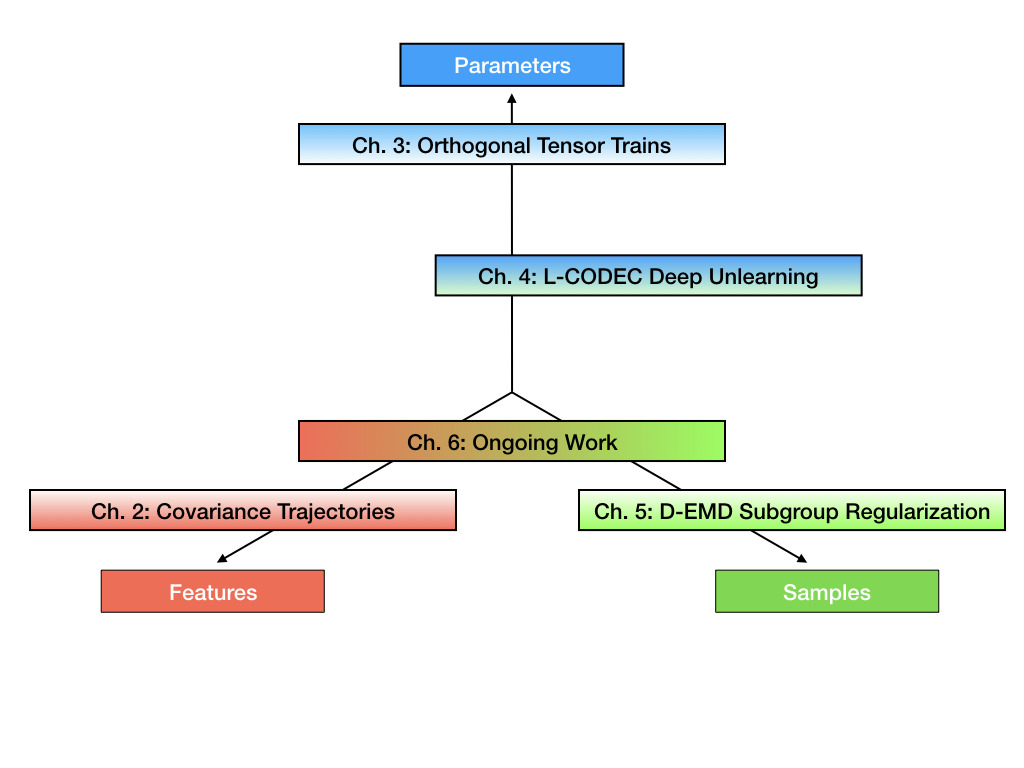
\includegraphics[width=0.95\linewidth]{diss/1_intro/figs/thesis_scope.png}
    \caption[Thesis Scope]{Thesis scope, projected over three representative axes. {\color{red} update chapter numbers shift by 1}}
    \label{fig:scope}
\end{figure}

\subsection{Second-Order Modeling and Group Difference Analysis over Time}

Recent results in coupled or temporal graphical models offer schemes for estimating the relationship structure 
between features when the data come from
related (but distinct) longitudinal sources. A novel application of these ideas is for analyzing group-level differences, i.e., in identifying if {\em trends} of estimated objects (e.g., 
covariance or precision matrices) are different across disparate conditions (e.g., gender or disease). Often, poor effect sizes make detecting the \textit{differential} signal 
over the {\em full} set of features difficult: for example, 
dependencies between only a {\em subset of features} may manifest differently across groups.
We first suggest
a parametric model 
for estimating trends in the space of $\SPD$ matrices as a function of one or more covariates.
We will then generalize scan statistics to graph structures, 
to search over distinct subsets of features (graph partitions) whose temporal dependency structure may show statistically 
significant group-wise differences.
We will theoretically analyze the Family Wise Error Rate (FWER) and bounds on Type 1 and Type 2 error. 
On a cohort of individuals with risk factors for Alzheimer's disease (but otherwise cognitively healthy), 
we 
find scientifically interesting 
group differences where the default analysis, 
i.e., models estimated on the full set of features, do not survive reasonable 
significance thresholds. 
% Preliminary work on this was published in \citep{covtraj}.


\subsection{Efficient Tensor Representations for Feasible Temporal Deep Learning}

Modern deep networks have proven to be very effective for analyzing real world images.
However, their application in medical imaging is still in its early stages,
primarily due to the large dimension of three-dimensional images, requiring enormous convolutional or fully connected layers --
if we treat an image (and not image patches) as a sample. 
These issues only compound when the focus moves towards longitudinal analysis
through recurrent structures, and when a point estimate of model parameters is insufficient 
in scientific applications where a reliability measure is necessary.
Using insights from differential geometry, 
we will adapt 
the tensor train decomposition to construct networks
with significantly fewer parameters,
allowing us to train powerful recurrent networks on whole brain image volumes. 
We analyze 
the \textit{orthogonal tensor train},
and demonstrate its ability to express a standard network layer both theoretically and empirically.
We 
demonstrate its ability to 
effectively reconstruct whole brain volumes
with faster convergence and stronger confidence intervals
compared to the standard tensor train decomposition. 
We provide code and show experiments on the ADNI dataset
using image sequences to regress on a cognition related outcome.
% Preliminary work on this was published in \citep{ott}.

\subsection{Practical Unlearning via Large-Scale Conditional Independence Testing}

%With AI systems extensively using personal %data for model training, 
Recent legislation has
led to interest in {\em machine unlearning}, i.e., removing specific training samples from a {\em predictive} model as if they never existed in the training dataset. 
Unlearning may also be required due to  corrupted/adversarial data or simply a user's updated privacy requirement.
For models which require no training ($k$-NN), 
simply deleting the closest original sample can be effective. 
%However, it is not clear how such approaches can be used to unlearn 
%models that contain rich information learned from the original data.
But this idea is inapplicable to models which learn richer 
representations.
%from data. 
%Recently, optimization-based unlearning estimators have been proposed, but 5their 
Recent ideas leveraging optimization-based updates
scale poorly with the model dimension $d$,  
due to 
inverting the Hessian of the loss function. %with an overall cost of $O(d^3)$ 
%is prohibitive.
We describe
a variant of a new conditional independence coefficient, 
L-CODEC, to identify a subset of the model parameters with the most semantic overlap on an individual sample level. 
Our approach completely avoids the need to invert a (possibly) huge matrix. 
By utilizing a Markov blanket selection, 
we find
that L-CODEC is also suitable for deep unlearning,
as well as other applications in vision.
Compared to alternatives, L-CODEC makes approximate unlearning possible 
in settings that would otherwise be infeasible, 
including vision models used for face recognition, 
person re-identification 
and NLP models that may require unlearning samples identified for exclusion.
% Preliminary work on this will appear in \citep{lcodec}.


\subsection{Reducing Subgroup Fairness via High Dimensional Earth Mover's Distances}

Optimal transport has recently emerged as a useful tool for machine learning through its connections with geometry, statistical machine learning, and through practical algorithms. Existing methods that leverage optimal transport often  regularize using  a Wasserstein metric or by computing barycenters, for example. %which are effective when distributions are continuous and known, or when measures of interest are discrete.
% Our formulation allows for a discretization of continuous measures that drop in directly to classical  formulations of the Earth Mover's Distance. 
We leverage optimal transport, except that we take advantage of a recently-introduced algorithm that computes a generalized earth mover's distance.
Not only is this algorithm computationally cheaper to compute compared to existing barycentric measures, but our method has the additional  advantage that gradients used for backpropagation can be directly read off of the forward pass computation, which leads to substantially faster model training.
We provide technical details about this new regularization term and its properties, 
and 
experimental demonstrations of improved training speed over existing Wasserstein-style methods.

{\color{red}
\subsection{Understanding Latent Spaces via Conditional Independences}

The final chapter of this thesis applies some of the tools developed above in the analysis of latent spaces in recent large scale models.
% In these studies, 
% we aim to identify conditionally independent features and subjects that are particularly important to the prediction and estimation of
% key disease outcomes,
% as a function of a number 
% of demographic, neuropsychological,
% genetic,
% and imaging data collected as 
% part of an ongoing consortium 
% to understand the progression
% of Alzheimer's disease in younger, 
% asymptomatic populations.
% In what follows we present
% exploratory analysis
% on a small, easily 
% digestible subset of the available data,
% that lays the foundation for
% further analysis.
}
% This work is the most forward looking, and aims to be a stepping stone toward a rigorous 

\section{Outline}
Chapter 2 covers the essential background necessary for the developments presented in the following chapters, including specifics of graphs and hypothesis testing, as well as relevant modern methods for learning and optimization.
In Chapters 3 through 7, we describe four perspectives to address subset identification.
Chapter 3 explores and focuses on the identification of feature subsets varying over time.
In Chapter 4 we describe a method of constraining the parameter space in a particular manner
that enables more efficient large scale neural networks.
Next, Chapter 5 provides a solution to the machine unlearning problem,
enabled through a particular conditional independence parameter selection scheme, vastly reducing network update costs.
Chapter 6 ends with a unique solution to subgroup fairness, 
where we take advantage of an efficient solution to
the $d$-dimensional earth mover's problem
to regularize large models when the number of subgroups can be large.
{\color{red} Chapter 7 describes future work, focused on applying a particular solution from Chapter 5 to understanding relationships among features in latent spaces learned by large generative models.}


%%%%%%%%%%%%% 
% Some old stuff

% Significant progress in the modern development of machine learning has
% been built upon connections and patterns identified across myriad
% interdisciplinary fields of study.
% Up through the mid 2000's, 
% many of these methods were inspired by and interested in 
% highly focused and constrained problems. 
% With a reasonably sized input domain, could a model of roughly equal size be used to
% predict some output?
% Linear regressors, decision trees, and support vector machines were all answers to these questions, with their own
% varying degrees of scaling and complexity.
% These methods necessitated carefully constructed formulations with specific restrictions to the learnable function class,
% enabling straightforward analysis 
% for provable performance guarantees 
% and easy identification of critical training samples and important input features.

% Contemporary machine learning, however, has a vastly different modus operandi. 
% Driven in large part by the exponential growth of available computation via Moore's Law, \textit{deep learning} has fallen squarely in the realm of \textbf{over-parameterized} models.
% With these overparametrizations and computation capacity, the typical learning questions posed as maximizing accuracy or reducing error have largely been addressed for even large scale problems.
% As such, complementary questions have led to subfields focusing on other performance measures, such as robustness, fairness, interpretability, and explainability.
% Many solutions to these questions end up looking back at answers found for the under- or non-parametrized settings.
% While nascent, these approaches 
% attempt to fill the gap between
% statistical and deep models to enable similar measures of sample influence, feature importance, and model analysis. 
% Most notable amongst these newer approaches is that of (Self)-Attention in Neural Networks \citep{sutskever2014sequence,vaswani2017attention}.
% Other proposals 
% end up looking back at the types of analysis typical of those more classical under-parametrized or nonparametrized methods.

% Not limited to previous developments in learning or computation theory, the arguably most valuable contributions toward the exponential reduction in model error can be attributed to influences and intuitions taken
% from biology, psychology, neuroscience, and even XXX \citep{srivastava, etc}.
% Perhaps one explanation as to why this phenomenon exists may be attributed to the way in which deep learning evolved. 
% The classical learning goal of function approximation lends itself nicely to a system which allows for arbitrary complexity via simple changes (e.g., addition of neural network layers). % Foundational works building on the original neural networks particularly have taken advantage of constraining this space of functions to search over: 
% the most seminal case being those of convolutional filters for imaging data. 
% While ``constraints" of this form have helped tremendously in model performance on modern vision and language machine learning tasks (GANs, Recurrent Networks, Residual Layers, Transformers, etc.), the ability to identify \textit{subsets} of important samples, input features, and model parameters has lagged significantly behind the development of these methods.
% Recently larger interest has been taken by the community to understand and interpret models with this view, only after extremely large and opaque models have become ubiquitous.
%This lag directly explains the more recent interest in developing methods for understanding and interpreting large scale machine learning models. % COVTRAJ
% \chapter{Introduction} \label{chap:intro} 

Modern applications of machine learning in a broad range of industrial and consumer-facing systems have become ubiquitous.
Most interactions with daily technologies now intrinsically involve 
a request to some ``smart`` system in the ``cloud'', 
where those interactions range from
a request for map directions 
to simply loading a webpage.
Neural network models, and the recent advances of deep learning,
have enabled these systems that 
make such applications possible.
These models have achieved
human-level performance on learning tasks
including image classification~\citep{resnet,alexnet}, image segmentation~\citep{segmentation}, video analysis~\citep{zhang2016video}, text understanding and generation~\citep{bert,gpt}, and have slowly begun to solve more fundamental scientific problems such as protein folding~\citep{protein} drug discovery~\citep{drugdisc}, and medical diagnosis~\citep{diag}.
While this performance is largely attributed to model size,
the abundance of high quality training data
has equally contributed to real world performance,
enabling model training over millions of real world samples~\citep{imagenet,laion},
and potentially billions of synthetic samples via environment simulation~\citep{mcts}.

While deployment in some domains (recommender systems, object detection) may benefit almost unconditionally from this vastly expanded capability, rightful hesitancy has limited their widespread use in particular applications where impacts on individuals, people, or environments may be at stake.
These ``last mile'' concerns take a few forms.
% Because a completely accurate model is still out of reach, an important question that needs to be answered is: which inputs or individuals are being given incorrect outcomes, and why?
% maybe a sentence suggesting unlearning/removal
In mission critical applications such as medical diagnosis, 
the impact of an error can be extremely large,
even if a misprediction happens extremely infrequently.
Additionally, large scale model training and architecture search
can require exorbitant amounts of energy producing high emissions,
and their scale can limit market participants
to only large actors with vast existing resources.
The accessibility and effectiveness of these models can also vary significantly based on the training data, and disparate outcomes can be exacerbated by existing social inequity.

While existing human or ``natural'' systems that these models aim to assist are not perfect, 
our real world has developed norms and regulations that 
enable them to function.
A medical diagnosis might require a physician to explain what symptoms led them to that particular conclusion.
Energy metering and carbon taxes may be applied to limit
emissions.
Regulatory satisfaction may require 
analysis proving equal opportunity,
or that specific protected classes
are not used in decision making.
% Specifically, these can include ideas as simple as the Hippocratic Oath and medical malpractice insurance, to asking your doctor what symptoms lead them to a particular diagnosis.
These ideas are difficult to directly translate to automated machine learning systems,
but proxies have been identified that we can build upon.

These norms and regulations answer a number of questions we may also try to pose to our machine learning models.
What is the cost to learn this task?
What led to this particular outcome?
Why is this outcome different from another?
% We will explore how these questions can be formulated concretely. 

If the answer to these questions is negative or unknown,  follow-up questions all take an interesting form:
Can we learn a smaller model with similar performance? 
Can we identify the most important features? 
Which individuals or groups are being treated unfairly, and can we change that?
These questions ask us to identify a \textit{subset} of some relevant set, dependent on setting, and this identification is our focus here.

% Moving specifically to machine learning methods,
Taking a step back, let's take a look at a representative system. Figure~\ref{fig:dl} illustrates a typical learning pipeline. 
A dataset is collected and used to train a model, by minimizing the error over
those samples in the dataset (top).
A ``sample'' can be a single measured value, or it can
be a large, highly structured object with many ``features.''
The model is made up of some ``parameters'' that are 
tuned during training to learn a good predictor over the training dataset.
This model is then used to predict, or \textit{infer}, on new
data seen ``in the wild'' (bottom).
Our questions above are formally asking to identify \textit{subsets of these objects}: is a subset of the model parameters sufficient for learning? Which subset of the features are important for a prediction? Which subset of the dataset exhibit a specific attribute?
\begin{figure}
    \centering
    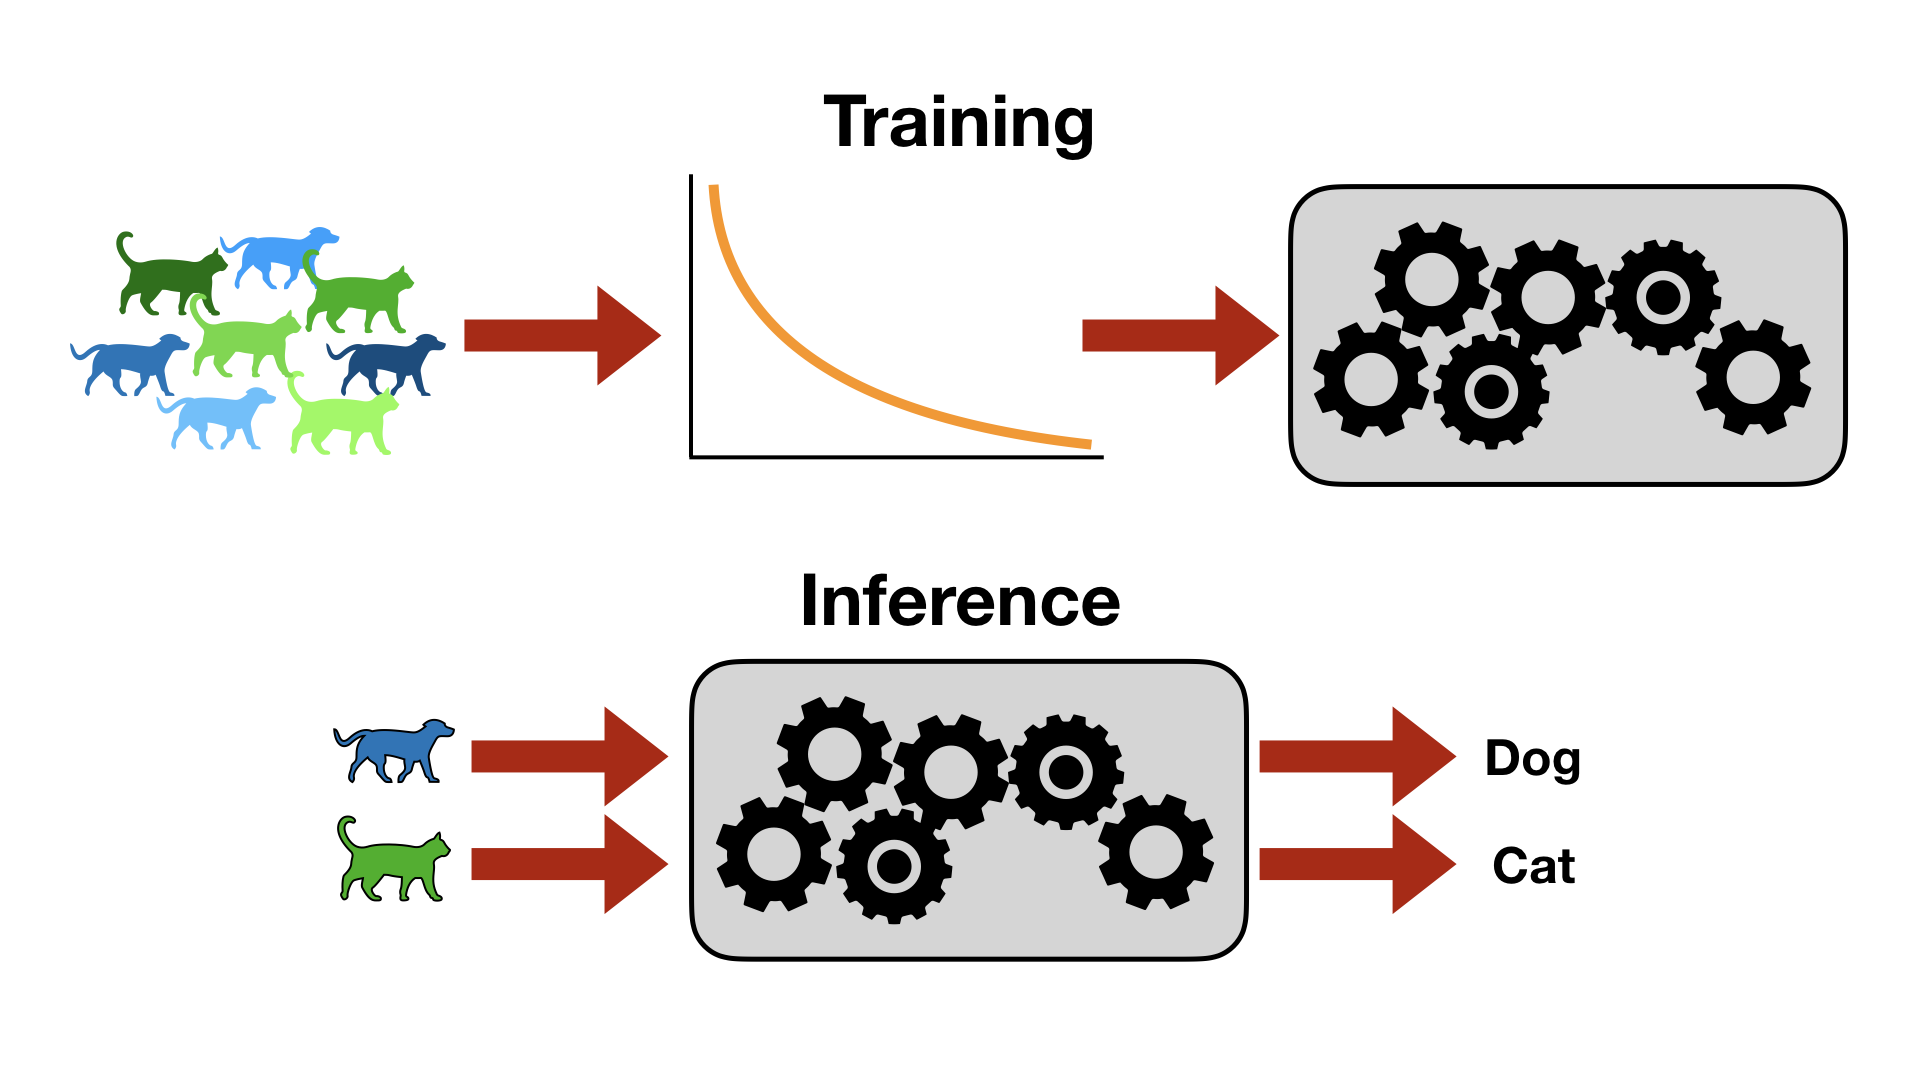
\includegraphics[trim={0 3cm 0 3cm},clip,width=0.95\textwidth]{diss/1_intro/figs/dl.png}
    \caption[Modern machine learning pipelines]{Machine learning training and inference visualization.}
    \label{fig:dl}
\end{figure}

% \textit{Explainability} can be seen as identifying important features of the input, as well as parts of the model (parameters) that ``light up`` for that input. \textit{Fairness} can be evaluated via measures over subsets of the data that correspond to specific groups. 

\begin{mdframed}[style=MyFrame]
\em 
\textbf{This thesis} focuses its main efforts on identifying these important subsets of model, feature, and sample space, to enable answering questions necessary for mainstream adoption of machine learning methods.
\end{mdframed}

% In this dissertation, we explore the sizes of these models, samples, and datasets, and 
% analyze under what situations 
% a smaller \textit{subset} of them may be sufficient or important
% for questions that run parallel to standard performance and accuracy measures.

Let us step a bit deeper into a basic illustrative example. In order to ease understanding, we can first begin with a basic formulation of learning methods, from which the questions above can take specific forms. 
Learning methods typically  try to identify a function mapping (model) that is able to complete a specific task at some high level of profficiency.
% In Figure~\ref{fig:dl}, a model is trained using examples of classification task (top), in order to accurately predict the class of a newly provided input (bottom).
% \begin{figure}
%     \centering
%     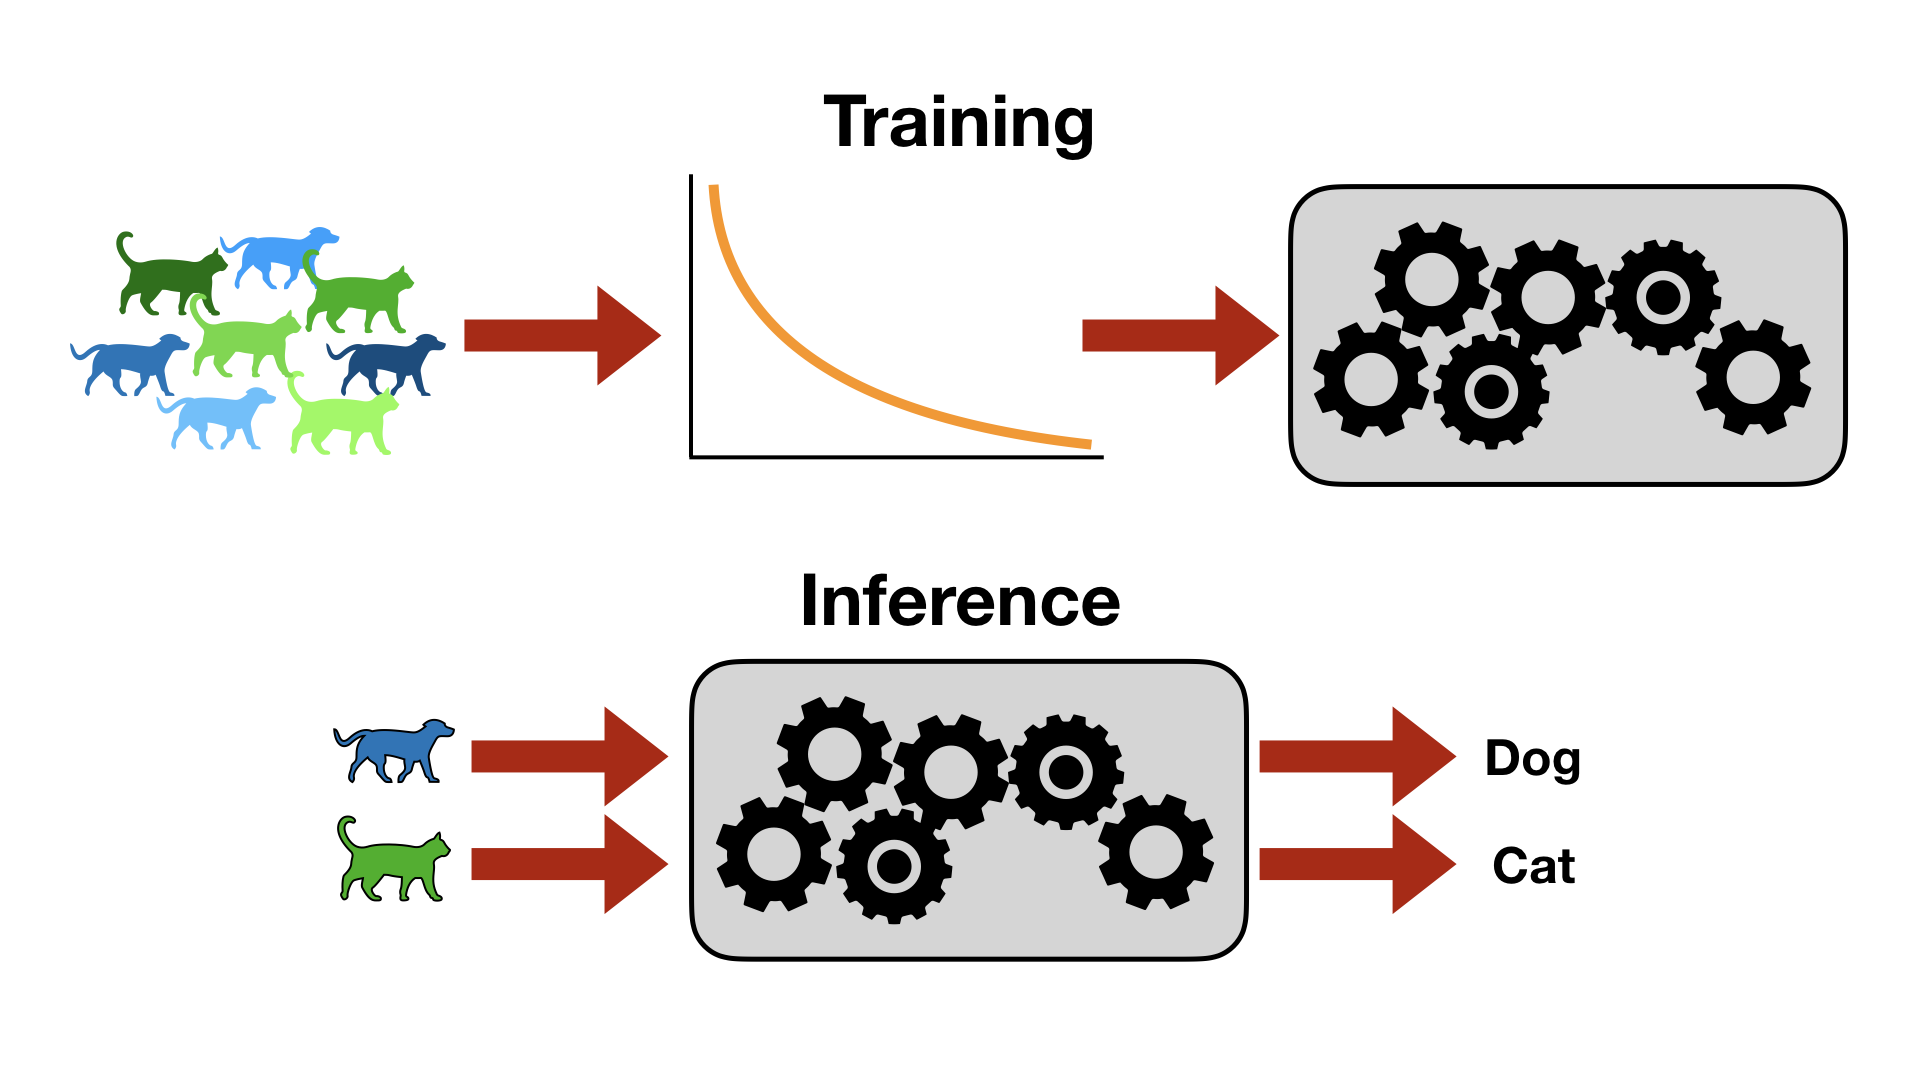
\includegraphics[trim={0 3cm 0 3cm},clip,width=0.95\textwidth]{diss/1_intro/figs/dl.png}
%     \caption[Modern machine learning pipelines]{Machine learning training and inference visualization.}
%     \label{fig:dl}
% \end{figure}
Say we have some dataset comprising of sample pairs $(x,y)$, where we wish to predict $y$ from $x$.
Our prediction, say $\hat{y}$, might be the output of some unknown function $f$ that we attempt to learn from training data. 
Let our approximation to this function be $\hat{y}:=\hat{f}(x)$.
This can take many forms, 
based on assumptions and prior information we may have on the relationships among the data. 
Consider the simple \textit{linear} case,
where we want to learn some parameter $w$ such that $y = w\cdot x$. 
Given $n$ sample pairs $(x_i,y_i)$ indexed by $i$, traditional statistics and optimization literature yield the following \textit{least squares} problem formulation, where we want to minimize the ``squared error'' between the observed values $y_i$ and the predicted $\hat{y}_i:= w\cdot x_i$:
\begin{align}\label{eq:lq}
\hat{f}:=\hat{w} = \mathop{\arg\min}_{w} \sum_{i=1}^n (y_i - w\cdot x_i)^2
\end{align}
This formulation expands without much change to a multi-dimensional form of the input $x$ and respectively, $w$: the canonical case where a number of features, or \textit{covariates} (e.g., symptoms), are used together to predict the outcome (e.g., diagnosis). 
If we are interested in which features of $x$ are important, we can look at the relative values of the learned ``weights'' $w$. In this simple setting, the importance of a feature (say $x^j$) can be exactly determined by the importance of the parameter ($w^j$).
A weight value far from zero may indicate that corresponding feature is important for diagnosis.
% If instead we are interested in which samples are most important, we can use existing methods for sample reweighting or methods that use standard assumptions to efficiently identify important subsets.

In this case and others, traditional statistical learning methods 
have been studied 
for many decades.
Linear regressors, decision trees, and support vector machines
have all been analyzed under these lenses.
% ,
% and as the modern machine learning community
% has returned to these questions recently,
% so has a renewed interest in their methods of analysis.
New research focuses
particularly on the differences
associated with moving from classical \textit{under-parametrized} models to
modern (deep) \textbf{over-parameterized} models: where
the model size vastly outnumbers the number
of input samples.
% , and may even be comparable to 
% the \textit{entire sample space.}
Methods for estimating the number of samples needed,
the time to learn a particular task,
and the generalization ability 
all require new perspectives in this regime.
While nascent, this research
attempts to fill the gap between
statistical and deep models to enable similar measures of sample influence, feature importance, and model understanding. 

\paragraph{A full picture.}
Let us expand our notation from the example above to consider this more general framing.
Consider a dataset $X:=\{x_i\}_{i=1}^n$ of size $n$ where each data point $x_i$ in the set $X$ is drawn from some underlying distribution over the domain $x_i \sim \cX^d$, 
with domain dimensionality (number of features) $d$.
A model $f$ is fit using a parametrization $\theta \in \Theta$,
with $\Theta$ the space of possible parametrizations (models) with some intrinsic dimension $p$. 
%While all three of these problems are closely related, they require different approaches. 
Generalizing the least squares``error measure'' from Eq.~\eqref{eq:lq} to an arbitrary \textit{loss} $\ell$, we have
\begin{align}\label{eq:learning}
    \hat{f}:=\hat{\theta} = \mathop{\arg\min}_{\theta\in\Theta} \sum_{x \in X} \ell(f_\theta(x_i))
\end{align}
From an analysis perspective, 
we might be interested in any one of 
(a) subsets of input features $\cC \subseteq \cX$ that are important for the downstream task,
(b) associating model subsets $\cP \subseteq \Theta$ with specific inputs or groups of inputs, or 
(c) subsets or subgroups of samples $S \subseteq \{X\}$ that are sufficient or representative of the entire dataset.

Crucially, an uninformed search for a subset is computationally infeasible. For a superset of size $n=|X|$, The set of all subsets is the power set, with a size of $2^{n}$! If an identification procedure requires looking over all of these and choosing a ``best'' one by some metric, the procedure will be limited to very small supersets.
Efficient methods have been developed in each of the three contexts above to avoid this exponential search.

\begin{figure}
    \centering
    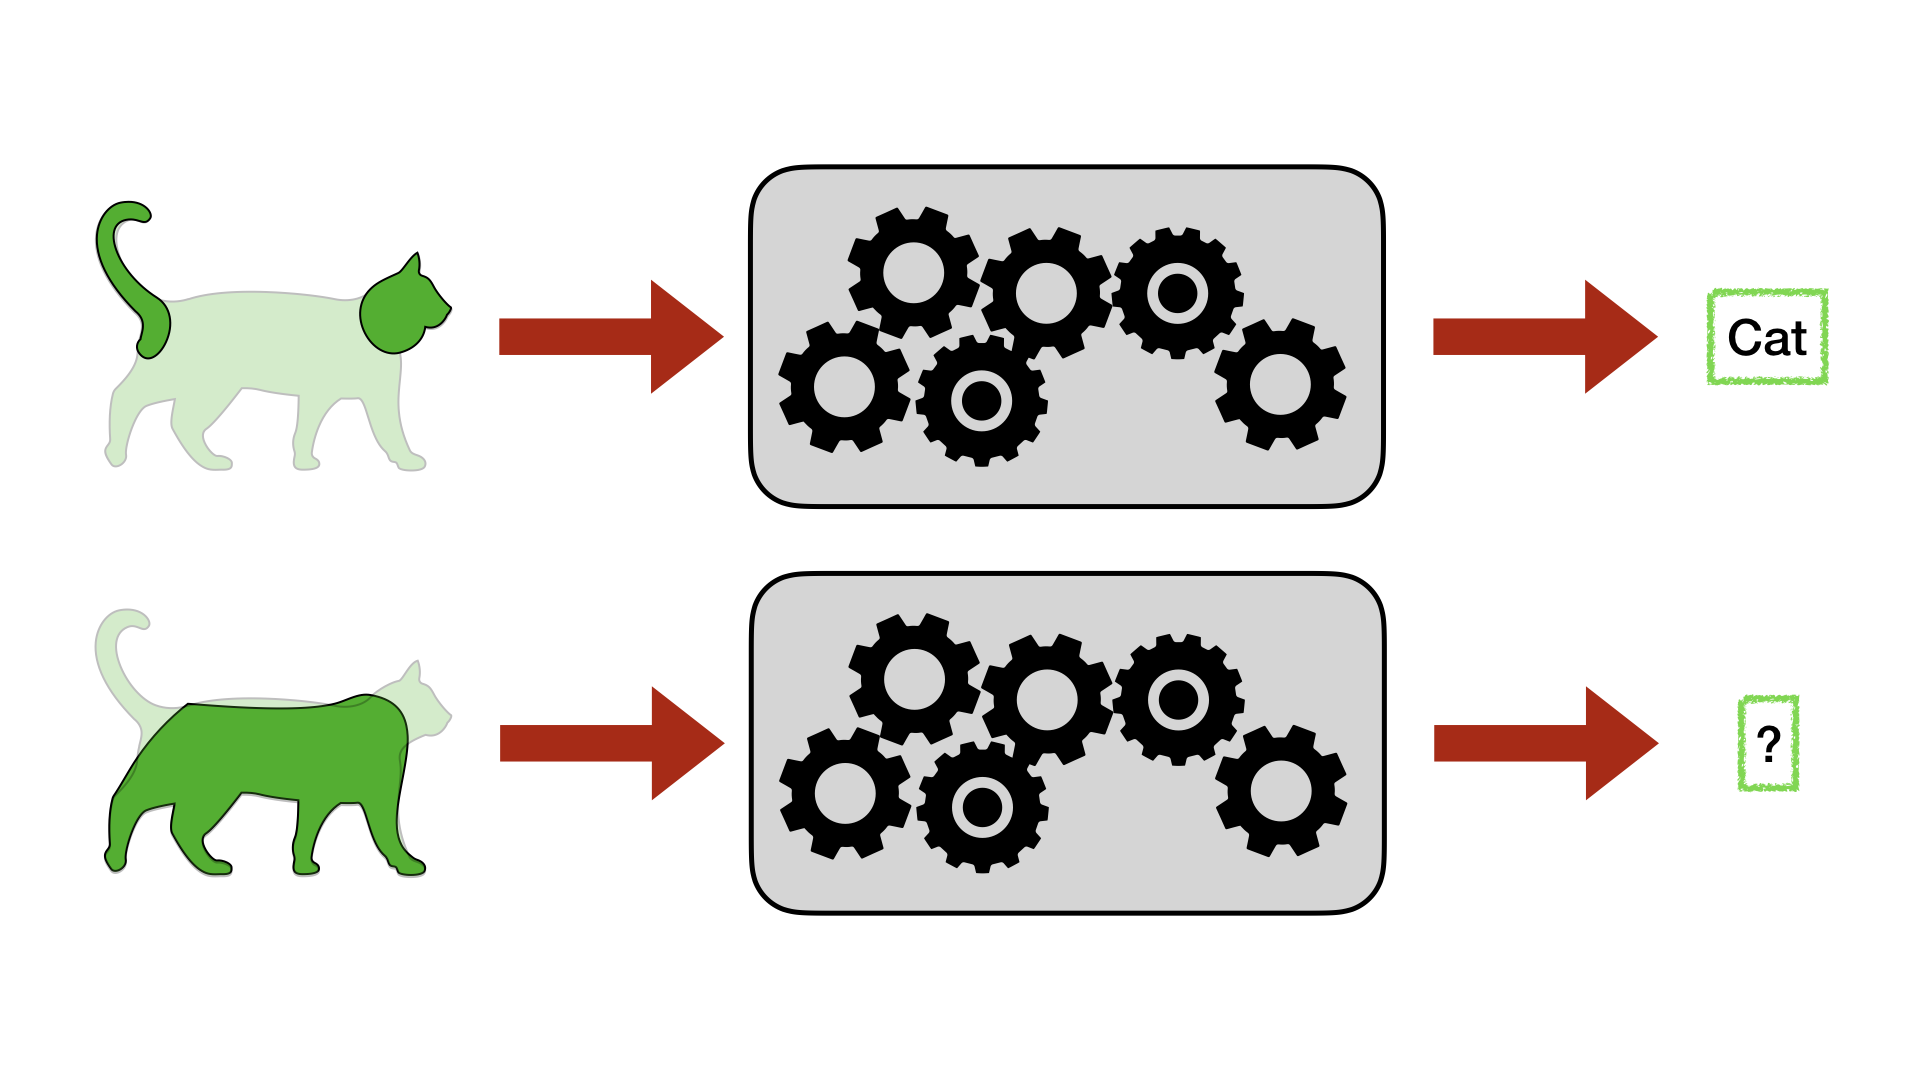
\includegraphics[trim={0 3cm 0 3cm},clip,width=0.9\textwidth]{diss/1_intro/figs/feat_select.png}
    \caption[Visualization of feature selection]{An example of identifying specific features important to the learning task.}
    \label{fig:feat_select}
\end{figure}
\paragraph{Feature Selection.} 
With more complex models $f$ compared to the linear case above, newer ``black-box'' methods have been developed for identifying important features. From the more pure statistics side, scan statistics~\citep{scanstat,scanstatlrt} allow for a structured ``scanning'' over the input space, skipping subsets unlikely to provide additional information for the measure of interest.
Further on the deep learning side, adaptations of sensitivity analysis, via noise addition and perturbations have found success~\citep{yeung2010sensitivity,zhang2015sensitivity}, alongside activation mapping~\citep{cam,selvaraju2017grad}.
These methods typically generate an analagous ``weighting'' over the input space, identifying features most salient for the specific task (Figure~\ref{fig:feat_select}).

\begin{figure}
    \centering
    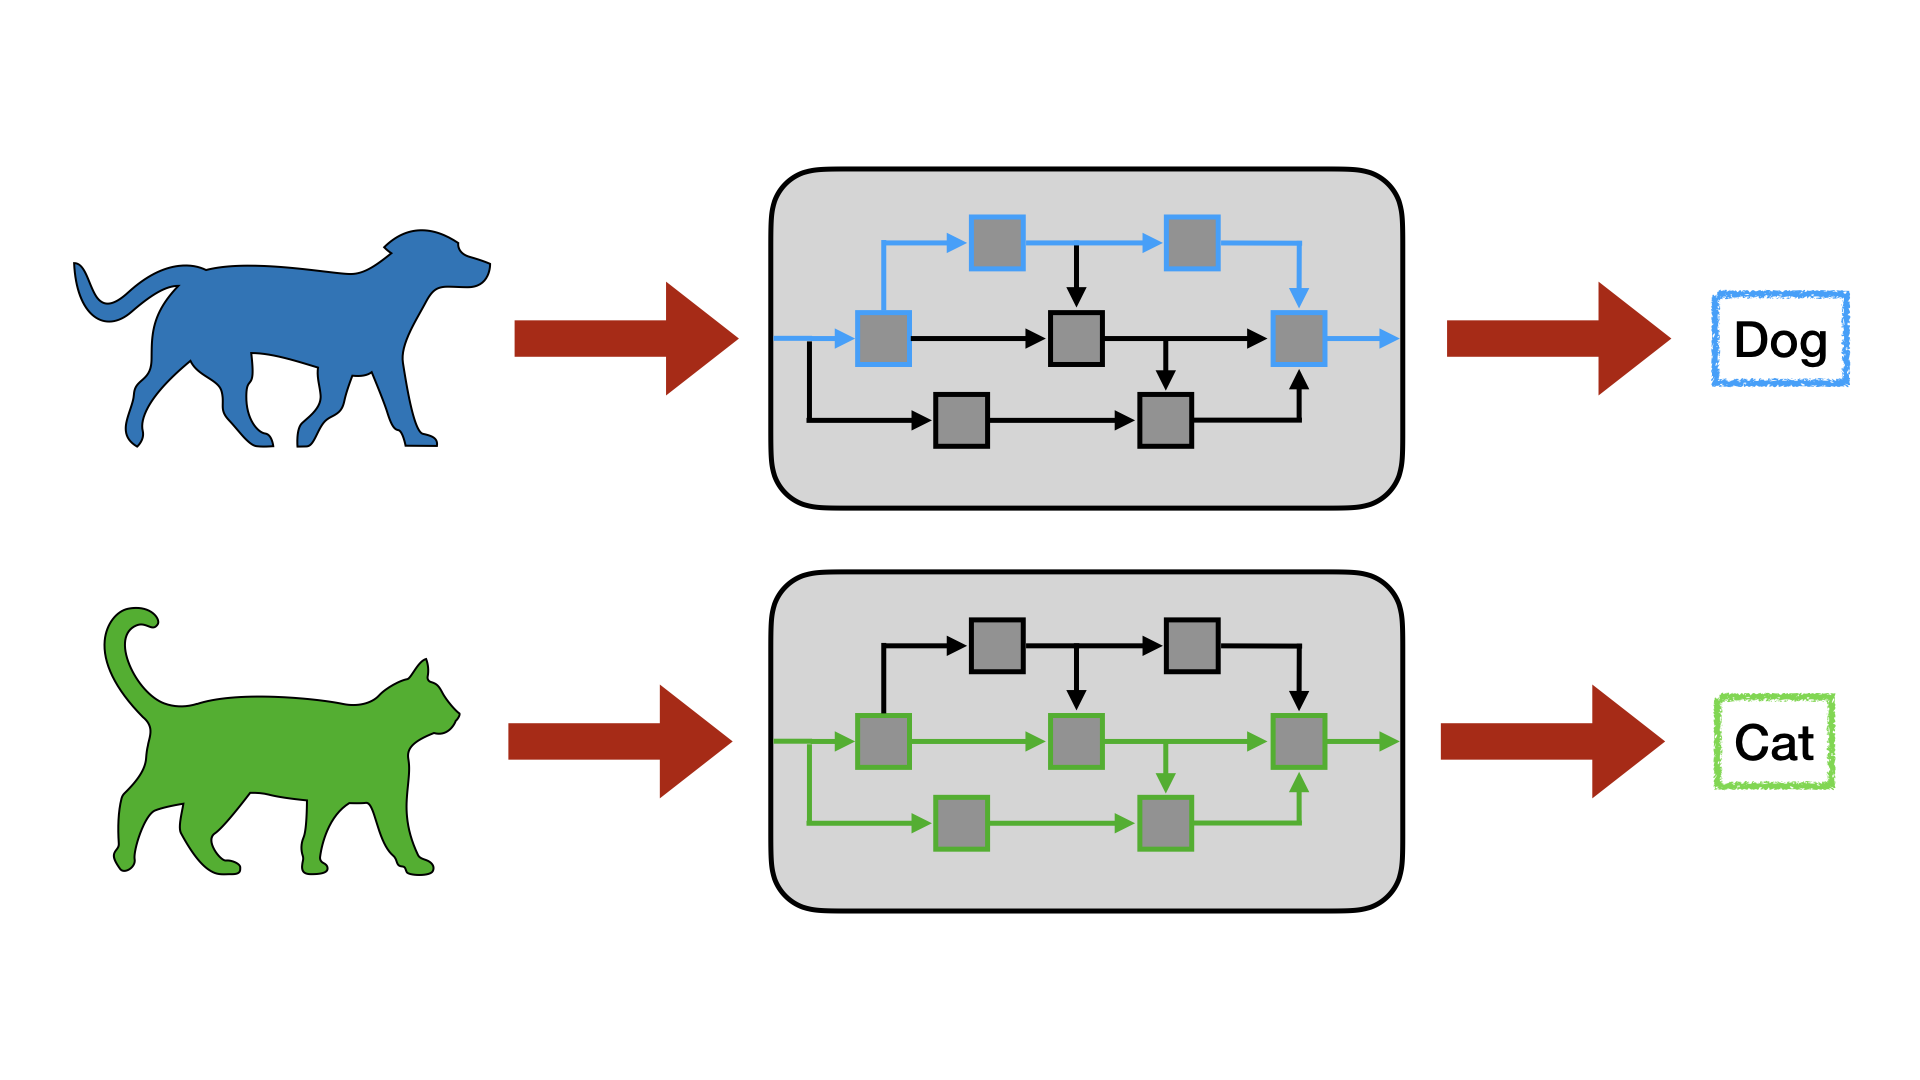
\includegraphics[trim={0 3cm 0 3cm},clip,width=0.9\textwidth]{diss/1_intro/figs/param_select.png}
    \caption[Visualization of parameter selection]{An example of identifying specific parameters important to the learning task.}
    \label{fig:param_select}
\end{figure}
\paragraph{Parameter Selection.} 
Selection in the model space generally takes two forms. First, as a prior, restriction, or assumption over the model space, and second, as a post-hoc method for an ``explainable'' proxy.
Regularization, sparsity, and gating methods are often used independent of the type or size of the model, to encourage the solution to fall within a specific region of the model space.
% In non-deep settings these methods come with strong theoretical guarantees. 
The theoretical underpinnings of these methods in deep learning are still being actively researched~\citep{hardt2016train,jacot2018neural,neyshabur2014search}, but the methods have nonetheless been effective in practice. 
On the post-hoc side, of particular interest are the parameters relevant to specific regions of the input space \textit{after} training (Figure~\ref{fig:param_select}). Here, recent analysis of deployed networks has shown this to be true~\citep{bau2017network,fong2018net2vec}, and current work continues to explore these network regions to aid in interpretability and explainability.

\paragraph{Sample Selection.} Many methods have been developed for outlier detection within training or testing sets~\citep{huang2020feature,ren2019likelihood} \textit{after} training, as well as methods for understanding sample influence~\citep{koh2017understanding,golatkar2020eternal,huang2020feature} . ``In-the-loop'' methods for accounting for ``outlierness'' behave similarly to accounting for group or individual fairness while training~\cite{mehrabi2021survey}. Unfortunately, once samples are identified in some manner, post-hoc adjustments to a trained model are generally very difficult. Recent work has focused on ``unlearning'', or removing a sample's influence on a model without retraining. If specific samples can be uniquely identified, performance and privacy reasons may require these specific interventions to reduce the ``influence'' of that sample subset.
\begin{figure}
    \centering
    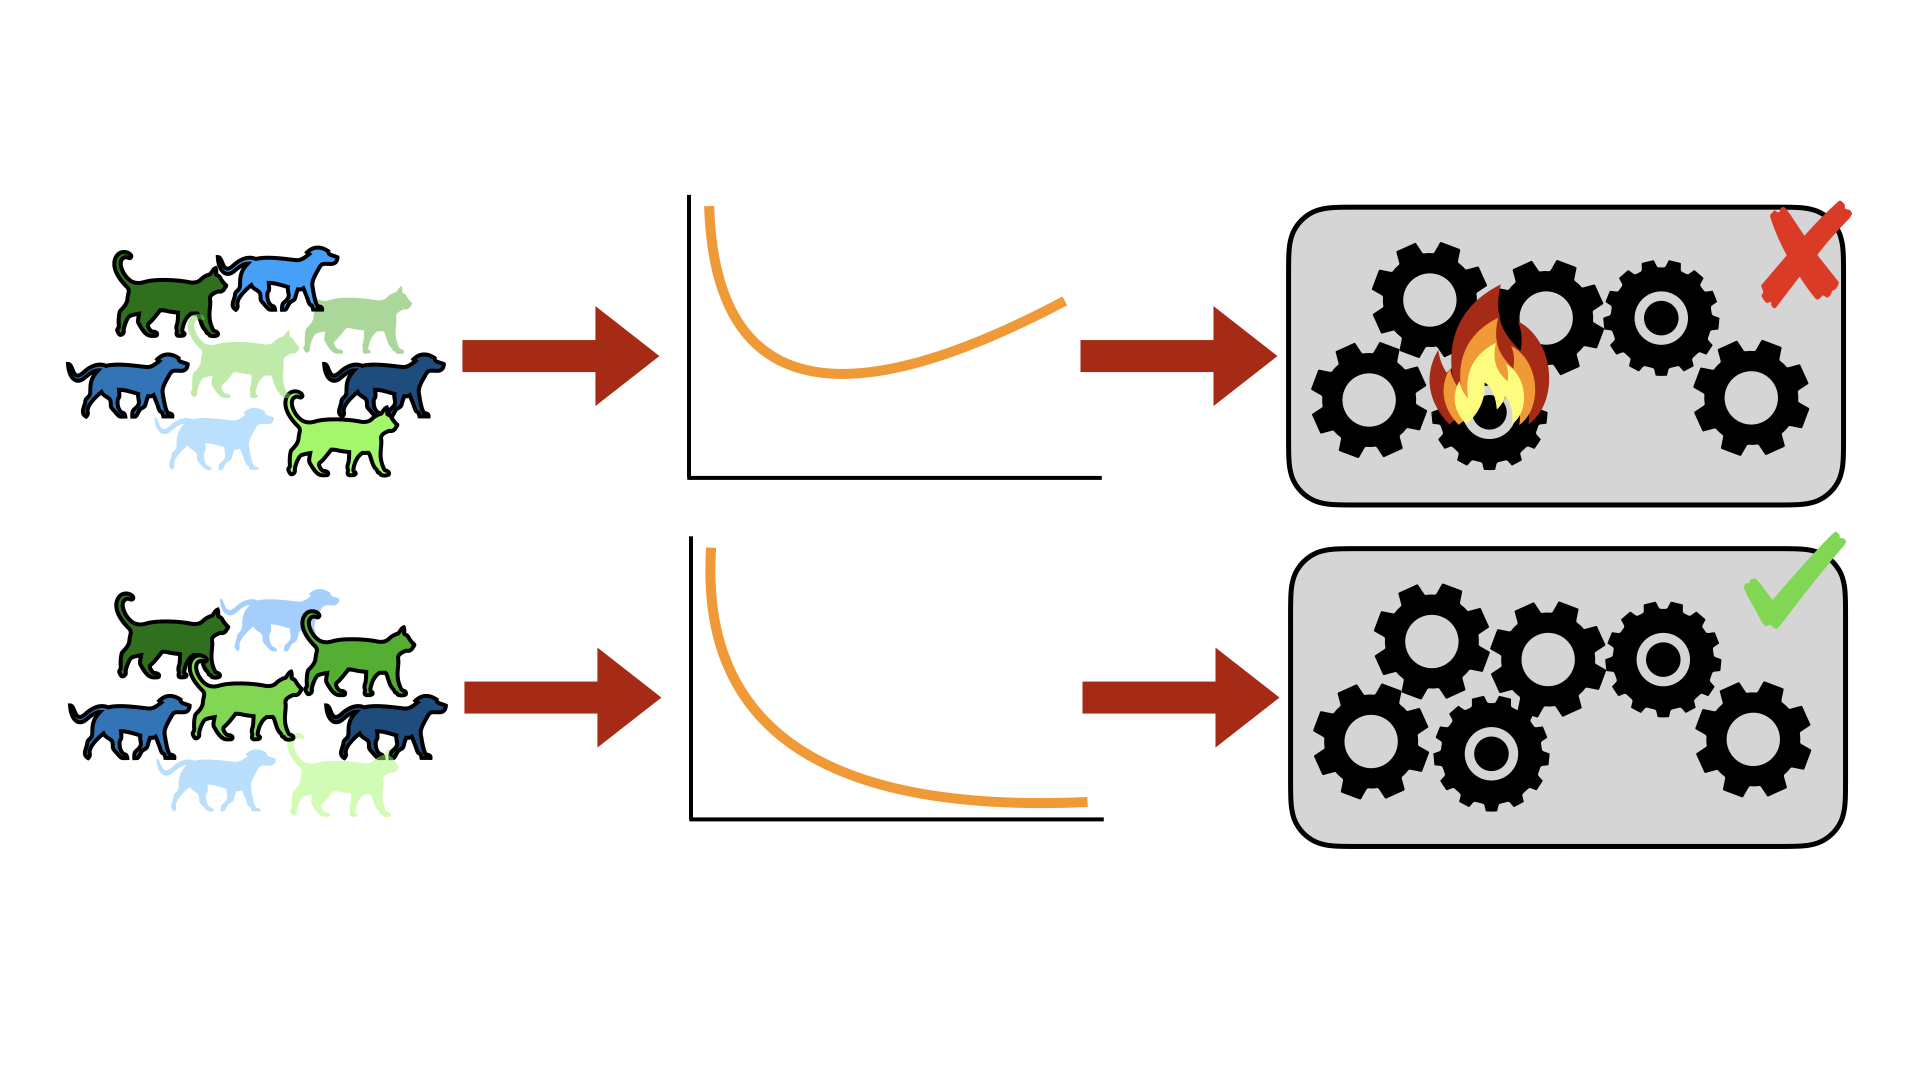
\includegraphics[trim={0 4.5cm 0 4cm},clip,width=0.9\textwidth]{diss/1_intro/figs/sample_select.png}
    \caption[Visualization of sample selection]{An example of identifying specific samples important to the learning task.}
    \label{fig:sample_select}
\end{figure}


\begin{mdframed}[style=MyFrame]
\textbf{ Thesis Goal: }
\em Identify, construct, and evaluate methods for \textbf{efficient} subset identification in modern machine learning feature, model, and input spaces.
\end{mdframed}

\section{A Few Motivating Examples}
Consider a traditional machine learning classification task in which we would like to predict whether an individual has a specific disease condition based on a medical resonance image (MRI) scan of their brain. Our input feature $x$ may consist of a 3D-array of values in $\RR^{\cI\times \cJ\times \cK}$ measuring some intensity of the imaging modality at each voxel, indexed by a tuple $(i,j,k) \in (\cI,\cJ,\cK)$.
Our outcome variable $y$ may simply be a binary label of whether the input scan has been labeled by a radiologist as one demonstrating typical disease characteristics.
Using an off the shelf 3D convolutional neural network with adjustments to match our input size, we can very quickly set up and train a system to predict disease presence with a high degree of accuracy.

\paragraph{Example 1.}
With a prediction for a specific scan, or predictions over a number of scans, we might be interested in identifying which regions of the brain are most important for diagnosis. These regions, $R \subset \cR:=\RR^{x\times y\times z}$, can be specific groups of pixels in the image that may correspond to known functional networks. Methods such as attention and class activation maps may work here, but there are a few issues. The number of samples available to learn a model is very small compared to the both the dimension of the input and the number of parameters in the model, i.e., $n \ll p$ and $n \ll d$. Thus it is very easy to overfit, and for areas of interest to be associated with intricacies of particular input data rather than true, real differences defined by the disease.

Furthermore, recent medical imaging studies have moved past simple difference detection: trends over time, and the ability to predict {\em future} disease development have by far become the setting of most interest.
Given an image of a healthy individual, is it possible to predict what their scan, or their future disease diagnosis, may be up to 10, 20, or more years in the future?
If a number of scans have been collected over some timeframe, can the \textit{trajectory} of the individuals' development be extrapolated to estimate progression?
As traditional models extended for temporal analysis grow in both size and complexity,
a number of subproblems explicitly related to model and input subspaces arise. In this thesis we address two such problems: \textbf{statistically rigorous identification of temporally evolving subsets}, and \textbf{characterizations of deep models that enable efficient training of recurrent models with large scale time-varying data}.
    
\paragraph{Example 2.}
With the rapid growth of AI and machine learning applications has come valid concerns regarding both guarantees of privacy.
Recent technology legislation has made the importance clear in all aspects of data use,
and particular projects and groups have demonstrated that machine learning is not independent of
this need \citep{Exposing}.
A new issue raised within this intersection is the ``right to be forgotten".
If a model has been trained with a particular users' data, 
they should have some recourse or right
to both remove their data from the training set,
and also know that the model has not learned from their data.
On the surface, this poses a significant problem for model builders
and organizations that spend large amounts
of time and resources in 
training deep learning models.

In the medical imaging example above this is especially important: with fewer samples it is more likely that information about any particular one could ``leak'', and the model's performance may degrade significantly as a relatively large percentage of it's training data is removed.
Thus tailored methods must be developed to ensure both privacy and performance, without requiring full retraining.
As we will see, 
\textbf{identification of model parameter subsets}
that are particularly important
for a particular sample's influence
in a model enables \textit{efficient machine unlearning}.

\paragraph{Example 3.}
From an alternative perspective, we may want to identify specific samples rather than have them specified a priori.
Traditionally a rigorous area of study under classical statistics, outlier detection and accounting have become a subfocus for many within the machine learning community as well \citep{golatkar2020eternal,golatkar2020forgetting,huang2020feature,ren2019likelihood}.
While subgroups of input samples may be outliers, it is more often the case that they represent known heterogeneity within the data. 
These differences may be marked using 
group information known a priori, and 
most learning tasks aim to learn tasks
in a \textit{subgroup-independent} manner.
In our disease prediction model above,
these groups could simply be stratified by the type of scanner used to acquire the image, but it could also
be a systematic difference correlated with some protected attribute. {\color{red} sentence about original brain atlas for registration being eurocentric}
This can directly lead to disparate performance and results on \textit{all} individuals outside of that group.
Optimization and regularization methods with this focus come under the umbrella of model fairness.
However, many existing methods do not scale well to larger models or as the number of subgroups grows, as is often the case when intersections of protected classes must be considered. Here we identify and construct a particular solution for \textbf{groupwise fairness that enables efficient in the loop fairness regularization}.

% What features are most important for prediction?
% Which samples were most important for my training?
% Can we understand when a model is certain or uncertain about its output?
% Are there layers in my network that have learned a particular subtask?
% Questions of robustness, bias, influence, fairness, and importance have become central questions to contemporary machine learning research \citep{doshi2017towards,mehrabi2021survey,amodei2016concrete}.
% machine learning, etc.

% Feature selection in the case of
% typical regression or classification 
% takes some form of learning parameters $\theta$ that allow for $\hat{y} = f_\theta(x)$ to be close to the true outcome of interest $y$.
% While forms of data $X := (x,y)$ may simply be continuous and real-valued, modern machine learning has greatly expanded formulations of the classical learning problem to include a wide variety of structured learning problems~\citep{nowozin2011structured}. 
% Consider the case when a high-dimensional input is used to predict an output with a highly-parametrized model. 
% Once learned, obvious questions arise as discussed above: are there specific low-dimensional spaces in either the input or the model space that are most important or necessary for the global learning problem of interest? Are there specific subspaces associated with particular subproblems of the global problem?
% The machine learning literature has come up with a number of ways to identify analogs of these spaces, 
% including extensions of sensitivity analysis to deep learning~\citep{yeung2010sensitivity,zhang2015sensitivity}, and constructing and identifying nonzero model subsets via particular model choices such as activations~\citep{selvaraju2017grad} and regularizers.
% In classical settings these are well understood: decision trees naturally provide ease of interpretibility via the information used to choose splits, and both linear and kernel support vector machines have been analyzed to provide for measures of sample importance via distances to the margin as well as feature importance via weights defining the learned hyperplane~\citep{Mitchell97}.
% Attention and saliency maps have emerged as popular new methods,
% given their ease of implementation and interpretation~\citep{sutskever2014sequence,vaswani2017attention,selvaraju2017grad}.
% By learning dimensions of a given input that are particularly important, either in a hard (binary) or soft (continuous weighting) manner, model builders are better able to understand and interpret what a model has learnt.
% The specific ideas of attention notwithstanding, many of these existing methods are far removed from traditional hypothesis testing frameworks.
% While some work has begun in this direction~\citep{tansey2018black},
% there remains a gap in direct identification of subsets and structures in these spaces that can be defined in statistically rigorous manners.

% \begin{figure}
%     \centering
%     \includegraphics[width=0.5\textwidth]{example-image-a}
%     \caption[A simple subset selection example]{\color{red} Identifying and selecting in MRIs, subset, sample, model ID.}
% \end{figure}

% \paragraph{A specific example.} 

% ------------------------------------------

% below here will be moved and arranged with the "selection" sections and here if relevant

% ------------------------------------------

% While attention can be directly applied to the network in order to identify ``hotspots" in the input space relating to the learned classification task, 
% given the high-dimensional nature of the input
% and the relatively small sample size 
% associated with medical imaging data, 
% it is very likely that an area of interest identified
% may be an intricacy of the training samples used rather than truly a region of disease signal.
% Class activation maps (CAMs) may be unclear, and can often associate with image artifacts unrelated to the scientific task~\citep{adebayo2018sanity}.
% Methods of generalization may help to increase confidence in identified regions, but statistical guarantees often remain out of reach.

% Furthermore, most recent problems associated with medical data have moved past simple difference detection: trends over time, and the ability to predict {\em future} disease development has by far become the setting of most interest.
% Given an image of a healthy individual, is it possible to predict what their scan, or their future disease diagnosis, may be up to 10, 20, or more years in the future?
% If a number of scans have been collected over some timeframe, can the \textit{trajectory} of the individuals' development be extrapolated to estimate progression?
% As traditional models extended for temporal analysis grow in both size and complexity,
% a number of subproblems explicitly related to model and input subspaces arise. Here we address two such problems: \textbf{statistically rigorous identification of temporally evolving subsets}, and \textbf{characterizations of deep models that enable efficient training of recurrent models with large scale time-varying data}.

% A sample's particular influence on model parameters aside, the identification of influential samples or subsets of samples more generally is of independent interest. 
% Traditionally a rigorous area of study under classical statistics, outlier detection and accounting have become a subfocus for many within the machine learning community as well \citep{golatkar2020eternal,golatkar2020forgetting,huang2020feature,ren2019likelihood}.
% While subgroups of input samples may be outliers, it is more often the case that they represent known heterogeneity within the data. 
% These differences are typically marked using 
% group information known a priori, and 
% most learning tasks aim to learn tasks
% in a \textit{subgroup-independent} manner.
% Optimization and regularization methods with this focus come under the umbrella of model fairness, and instead of identifying and boosting independences within the model or data, we aim to minimize them.
% However, many existing methods do not scale well as the number of subgroups grows, as is often the case when intersections of protected classes must be considered. In the sequel we identify and construct a particular solution for \textbf{groupwise fairness that enables efficient in the loop fairness regularization}.

\begin{mdframed}[style=MyFrame]
\em 
Here we focus our effort on identifying these important subsets of model, feature, and sample space for feature association, model size reduction, model unlearning, and, fairness. Specifically, taking advantage of both existing statistical and geometric methods, we develop new methods for localizing subsets in a range of settings from hypothesis testing to deep learning.
\end{mdframed}

\section{Thesis Scope and Contributions}

We explore the intersections of classical statistical and geometric constructions with modern machine learning methods. 
Figure~\ref{fig:scope} shows the overall scope projected along three axes: feature, parameter, and sample spaces.
Below we briefly introduce the main problems studied in this thesis.
\begin{figure}[!ht]
    \centering
    % \includegraphics[width=0.99\linewidth]{scope.pdf}
    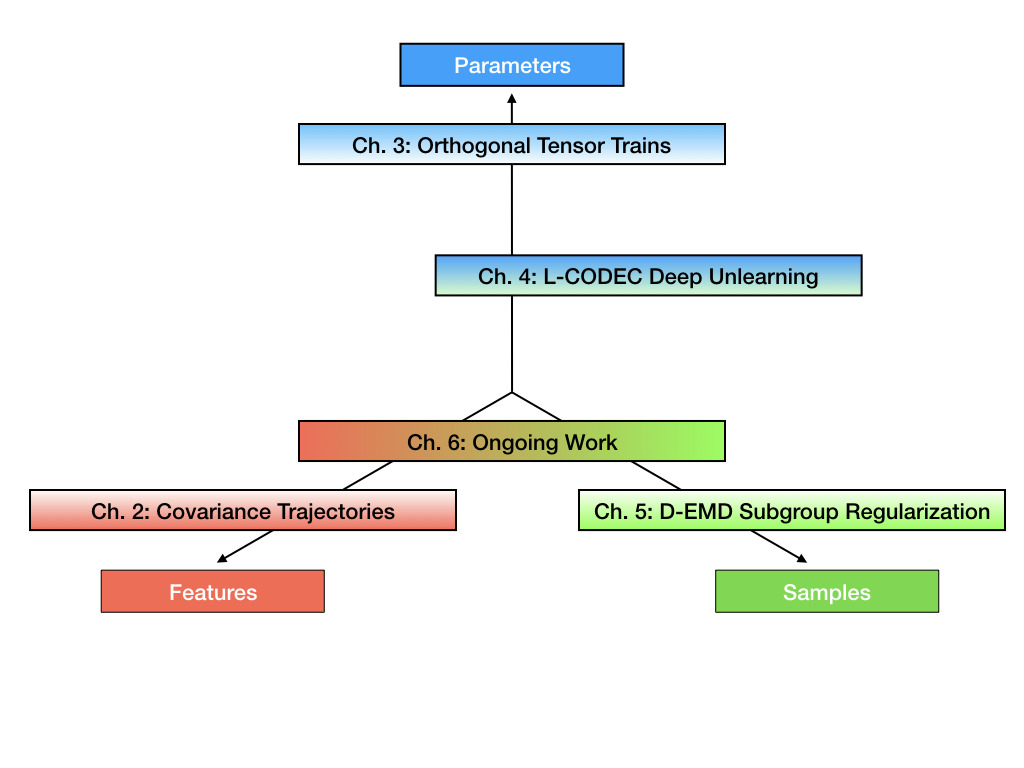
\includegraphics[width=0.95\linewidth]{diss/1_intro/figs/thesis_scope.png}
    \caption[Thesis Scope]{Thesis scope, projected over three representative axes. {\color{red} update chapter numbers shift by 1}}
    \label{fig:scope}
\end{figure}

\subsection{Second-Order Modeling and Group Difference Analysis over Time}

Recent results in coupled or temporal graphical models offer schemes for estimating the relationship structure 
between features when the data come from
related (but distinct) longitudinal sources. A novel application of these ideas is for analyzing group-level differences, i.e., in identifying if {\em trends} of estimated objects (e.g., 
covariance or precision matrices) are different across disparate conditions (e.g., gender or disease). Often, poor effect sizes make detecting the \textit{differential} signal 
over the {\em full} set of features difficult: for example, 
dependencies between only a {\em subset of features} may manifest differently across groups.
We first suggest
a parametric model 
for estimating trends in the space of $\SPD$ matrices as a function of one or more covariates.
We will then generalize scan statistics to graph structures, 
to search over distinct subsets of features (graph partitions) whose temporal dependency structure may show statistically 
significant group-wise differences.
We will theoretically analyze the Family Wise Error Rate (FWER) and bounds on Type 1 and Type 2 error. 
On a cohort of individuals with risk factors for Alzheimer's disease (but otherwise cognitively healthy), 
we 
find scientifically interesting 
group differences where the default analysis, 
i.e., models estimated on the full set of features, do not survive reasonable 
significance thresholds. 
% Preliminary work on this was published in \citep{covtraj}.


\subsection{Efficient Tensor Representations for Feasible Temporal Deep Learning}

Modern deep networks have proven to be very effective for analyzing real world images.
However, their application in medical imaging is still in its early stages,
primarily due to the large dimension of three-dimensional images, requiring enormous convolutional or fully connected layers --
if we treat an image (and not image patches) as a sample. 
These issues only compound when the focus moves towards longitudinal analysis
through recurrent structures, and when a point estimate of model parameters is insufficient 
in scientific applications where a reliability measure is necessary.
Using insights from differential geometry, 
we will adapt 
the tensor train decomposition to construct networks
with significantly fewer parameters,
allowing us to train powerful recurrent networks on whole brain image volumes. 
We analyze 
the \textit{orthogonal tensor train},
and demonstrate its ability to express a standard network layer both theoretically and empirically.
We 
demonstrate its ability to 
effectively reconstruct whole brain volumes
with faster convergence and stronger confidence intervals
compared to the standard tensor train decomposition. 
We provide code and show experiments on the ADNI dataset
using image sequences to regress on a cognition related outcome.
% Preliminary work on this was published in \citep{ott}.

\subsection{Practical Unlearning via Large-Scale Conditional Independence Testing}

%With AI systems extensively using personal %data for model training, 
Recent legislation has
led to interest in {\em machine unlearning}, i.e., removing specific training samples from a {\em predictive} model as if they never existed in the training dataset. 
Unlearning may also be required due to  corrupted/adversarial data or simply a user's updated privacy requirement.
For models which require no training ($k$-NN), 
simply deleting the closest original sample can be effective. 
%However, it is not clear how such approaches can be used to unlearn 
%models that contain rich information learned from the original data.
But this idea is inapplicable to models which learn richer 
representations.
%from data. 
%Recently, optimization-based unlearning estimators have been proposed, but 5their 
Recent ideas leveraging optimization-based updates
scale poorly with the model dimension $d$,  
due to 
inverting the Hessian of the loss function. %with an overall cost of $O(d^3)$ 
%is prohibitive.
We describe
a variant of a new conditional independence coefficient, 
L-CODEC, to identify a subset of the model parameters with the most semantic overlap on an individual sample level. 
Our approach completely avoids the need to invert a (possibly) huge matrix. 
By utilizing a Markov blanket selection, 
we find
that L-CODEC is also suitable for deep unlearning,
as well as other applications in vision.
Compared to alternatives, L-CODEC makes approximate unlearning possible 
in settings that would otherwise be infeasible, 
including vision models used for face recognition, 
person re-identification 
and NLP models that may require unlearning samples identified for exclusion.
% Preliminary work on this will appear in \citep{lcodec}.


\subsection{Reducing Subgroup Fairness via High Dimensional Earth Mover's Distances}

Optimal transport has recently emerged as a useful tool for machine learning through its connections with geometry, statistical machine learning, and through practical algorithms. Existing methods that leverage optimal transport often  regularize using  a Wasserstein metric or by computing barycenters, for example. %which are effective when distributions are continuous and known, or when measures of interest are discrete.
% Our formulation allows for a discretization of continuous measures that drop in directly to classical  formulations of the Earth Mover's Distance. 
We leverage optimal transport, except that we take advantage of a recently-introduced algorithm that computes a generalized earth mover's distance.
Not only is this algorithm computationally cheaper to compute compared to existing barycentric measures, but our method has the additional  advantage that gradients used for backpropagation can be directly read off of the forward pass computation, which leads to substantially faster model training.
We provide technical details about this new regularization term and its properties, 
and 
experimental demonstrations of improved training speed over existing Wasserstein-style methods.

{\color{red}
\subsection{Understanding Latent Spaces via Conditional Independences}

The final chapter of this thesis applies some of the tools developed above in the analysis of latent spaces in recent large scale models.
% In these studies, 
% we aim to identify conditionally independent features and subjects that are particularly important to the prediction and estimation of
% key disease outcomes,
% as a function of a number 
% of demographic, neuropsychological,
% genetic,
% and imaging data collected as 
% part of an ongoing consortium 
% to understand the progression
% of Alzheimer's disease in younger, 
% asymptomatic populations.
% In what follows we present
% exploratory analysis
% on a small, easily 
% digestible subset of the available data,
% that lays the foundation for
% further analysis.
}
% This work is the most forward looking, and aims to be a stepping stone toward a rigorous 

\section{Outline}
Chapter 2 covers the essential background necessary for the developments presented in the following chapters, including specifics of graphs and hypothesis testing, as well as relevant modern methods for learning and optimization.
In Chapters 3 through 7, we describe four perspectives to address subset identification.
Chapter 3 explores and focuses on the identification of feature subsets varying over time.
In Chapter 4 we describe a method of constraining the parameter space in a particular manner
that enables more efficient large scale neural networks.
Next, Chapter 5 provides a solution to the machine unlearning problem,
enabled through a particular conditional independence parameter selection scheme, vastly reducing network update costs.
Chapter 6 ends with a unique solution to subgroup fairness, 
where we take advantage of an efficient solution to
the $d$-dimensional earth mover's problem
to regularize large models when the number of subgroups can be large.
{\color{red} Chapter 7 describes future work, focused on applying a particular solution from Chapter 5 to understanding relationships among features in latent spaces learned by large generative models.}


%%%%%%%%%%%%% 
% Some old stuff

% Significant progress in the modern development of machine learning has
% been built upon connections and patterns identified across myriad
% interdisciplinary fields of study.
% Up through the mid 2000's, 
% many of these methods were inspired by and interested in 
% highly focused and constrained problems. 
% With a reasonably sized input domain, could a model of roughly equal size be used to
% predict some output?
% Linear regressors, decision trees, and support vector machines were all answers to these questions, with their own
% varying degrees of scaling and complexity.
% These methods necessitated carefully constructed formulations with specific restrictions to the learnable function class,
% enabling straightforward analysis 
% for provable performance guarantees 
% and easy identification of critical training samples and important input features.

% Contemporary machine learning, however, has a vastly different modus operandi. 
% Driven in large part by the exponential growth of available computation via Moore's Law, \textit{deep learning} has fallen squarely in the realm of \textbf{over-parameterized} models.
% With these overparametrizations and computation capacity, the typical learning questions posed as maximizing accuracy or reducing error have largely been addressed for even large scale problems.
% As such, complementary questions have led to subfields focusing on other performance measures, such as robustness, fairness, interpretability, and explainability.
% Many solutions to these questions end up looking back at answers found for the under- or non-parametrized settings.
% While nascent, these approaches 
% attempt to fill the gap between
% statistical and deep models to enable similar measures of sample influence, feature importance, and model analysis. 
% Most notable amongst these newer approaches is that of (Self)-Attention in Neural Networks \citep{sutskever2014sequence,vaswani2017attention}.
% Other proposals 
% end up looking back at the types of analysis typical of those more classical under-parametrized or nonparametrized methods.

% Not limited to previous developments in learning or computation theory, the arguably most valuable contributions toward the exponential reduction in model error can be attributed to influences and intuitions taken
% from biology, psychology, neuroscience, and even XXX \citep{srivastava, etc}.
% Perhaps one explanation as to why this phenomenon exists may be attributed to the way in which deep learning evolved. 
% The classical learning goal of function approximation lends itself nicely to a system which allows for arbitrary complexity via simple changes (e.g., addition of neural network layers). % Foundational works building on the original neural networks particularly have taken advantage of constraining this space of functions to search over: 
% the most seminal case being those of convolutional filters for imaging data. 
% While ``constraints" of this form have helped tremendously in model performance on modern vision and language machine learning tasks (GANs, Recurrent Networks, Residual Layers, Transformers, etc.), the ability to identify \textit{subsets} of important samples, input features, and model parameters has lagged significantly behind the development of these methods.
% Recently larger interest has been taken by the community to understand and interpret models with this view, only after extremely large and opaque models have become ubiquitous.
%This lag directly explains the more recent interest in developing methods for understanding and interpreting large scale machine learning models. % OTT
% \chapter{Introduction} \label{chap:intro} 

Modern applications of machine learning in a broad range of industrial and consumer-facing systems have become ubiquitous.
Most interactions with daily technologies now intrinsically involve 
a request to some ``smart`` system in the ``cloud'', 
where those interactions range from
a request for map directions 
to simply loading a webpage.
Neural network models, and the recent advances of deep learning,
have enabled these systems that 
make such applications possible.
These models have achieved
human-level performance on learning tasks
including image classification~\citep{resnet,alexnet}, image segmentation~\citep{segmentation}, video analysis~\citep{zhang2016video}, text understanding and generation~\citep{bert,gpt}, and have slowly begun to solve more fundamental scientific problems such as protein folding~\citep{protein} drug discovery~\citep{drugdisc}, and medical diagnosis~\citep{diag}.
While this performance is largely attributed to model size,
the abundance of high quality training data
has equally contributed to real world performance,
enabling model training over millions of real world samples~\citep{imagenet,laion},
and potentially billions of synthetic samples via environment simulation~\citep{mcts}.

While deployment in some domains (recommender systems, object detection) may benefit almost unconditionally from this vastly expanded capability, rightful hesitancy has limited their widespread use in particular applications where impacts on individuals, people, or environments may be at stake.
These ``last mile'' concerns take a few forms.
% Because a completely accurate model is still out of reach, an important question that needs to be answered is: which inputs or individuals are being given incorrect outcomes, and why?
% maybe a sentence suggesting unlearning/removal
In mission critical applications such as medical diagnosis, 
the impact of an error can be extremely large,
even if a misprediction happens extremely infrequently.
Additionally, large scale model training and architecture search
can require exorbitant amounts of energy producing high emissions,
and their scale can limit market participants
to only large actors with vast existing resources.
The accessibility and effectiveness of these models can also vary significantly based on the training data, and disparate outcomes can be exacerbated by existing social inequity.

While existing human or ``natural'' systems that these models aim to assist are not perfect, 
our real world has developed norms and regulations that 
enable them to function.
A medical diagnosis might require a physician to explain what symptoms led them to that particular conclusion.
Energy metering and carbon taxes may be applied to limit
emissions.
Regulatory satisfaction may require 
analysis proving equal opportunity,
or that specific protected classes
are not used in decision making.
% Specifically, these can include ideas as simple as the Hippocratic Oath and medical malpractice insurance, to asking your doctor what symptoms lead them to a particular diagnosis.
These ideas are difficult to directly translate to automated machine learning systems,
but proxies have been identified that we can build upon.

These norms and regulations answer a number of questions we may also try to pose to our machine learning models.
What is the cost to learn this task?
What led to this particular outcome?
Why is this outcome different from another?
% We will explore how these questions can be formulated concretely. 

If the answer to these questions is negative or unknown,  follow-up questions all take an interesting form:
Can we learn a smaller model with similar performance? 
Can we identify the most important features? 
Which individuals or groups are being treated unfairly, and can we change that?
These questions ask us to identify a \textit{subset} of some relevant set, dependent on setting, and this identification is our focus here.

% Moving specifically to machine learning methods,
Taking a step back, let's take a look at a representative system. Figure~\ref{fig:dl} illustrates a typical learning pipeline. 
A dataset is collected and used to train a model, by minimizing the error over
those samples in the dataset (top).
A ``sample'' can be a single measured value, or it can
be a large, highly structured object with many ``features.''
The model is made up of some ``parameters'' that are 
tuned during training to learn a good predictor over the training dataset.
This model is then used to predict, or \textit{infer}, on new
data seen ``in the wild'' (bottom).
Our questions above are formally asking to identify \textit{subsets of these objects}: is a subset of the model parameters sufficient for learning? Which subset of the features are important for a prediction? Which subset of the dataset exhibit a specific attribute?
\begin{figure}
    \centering
    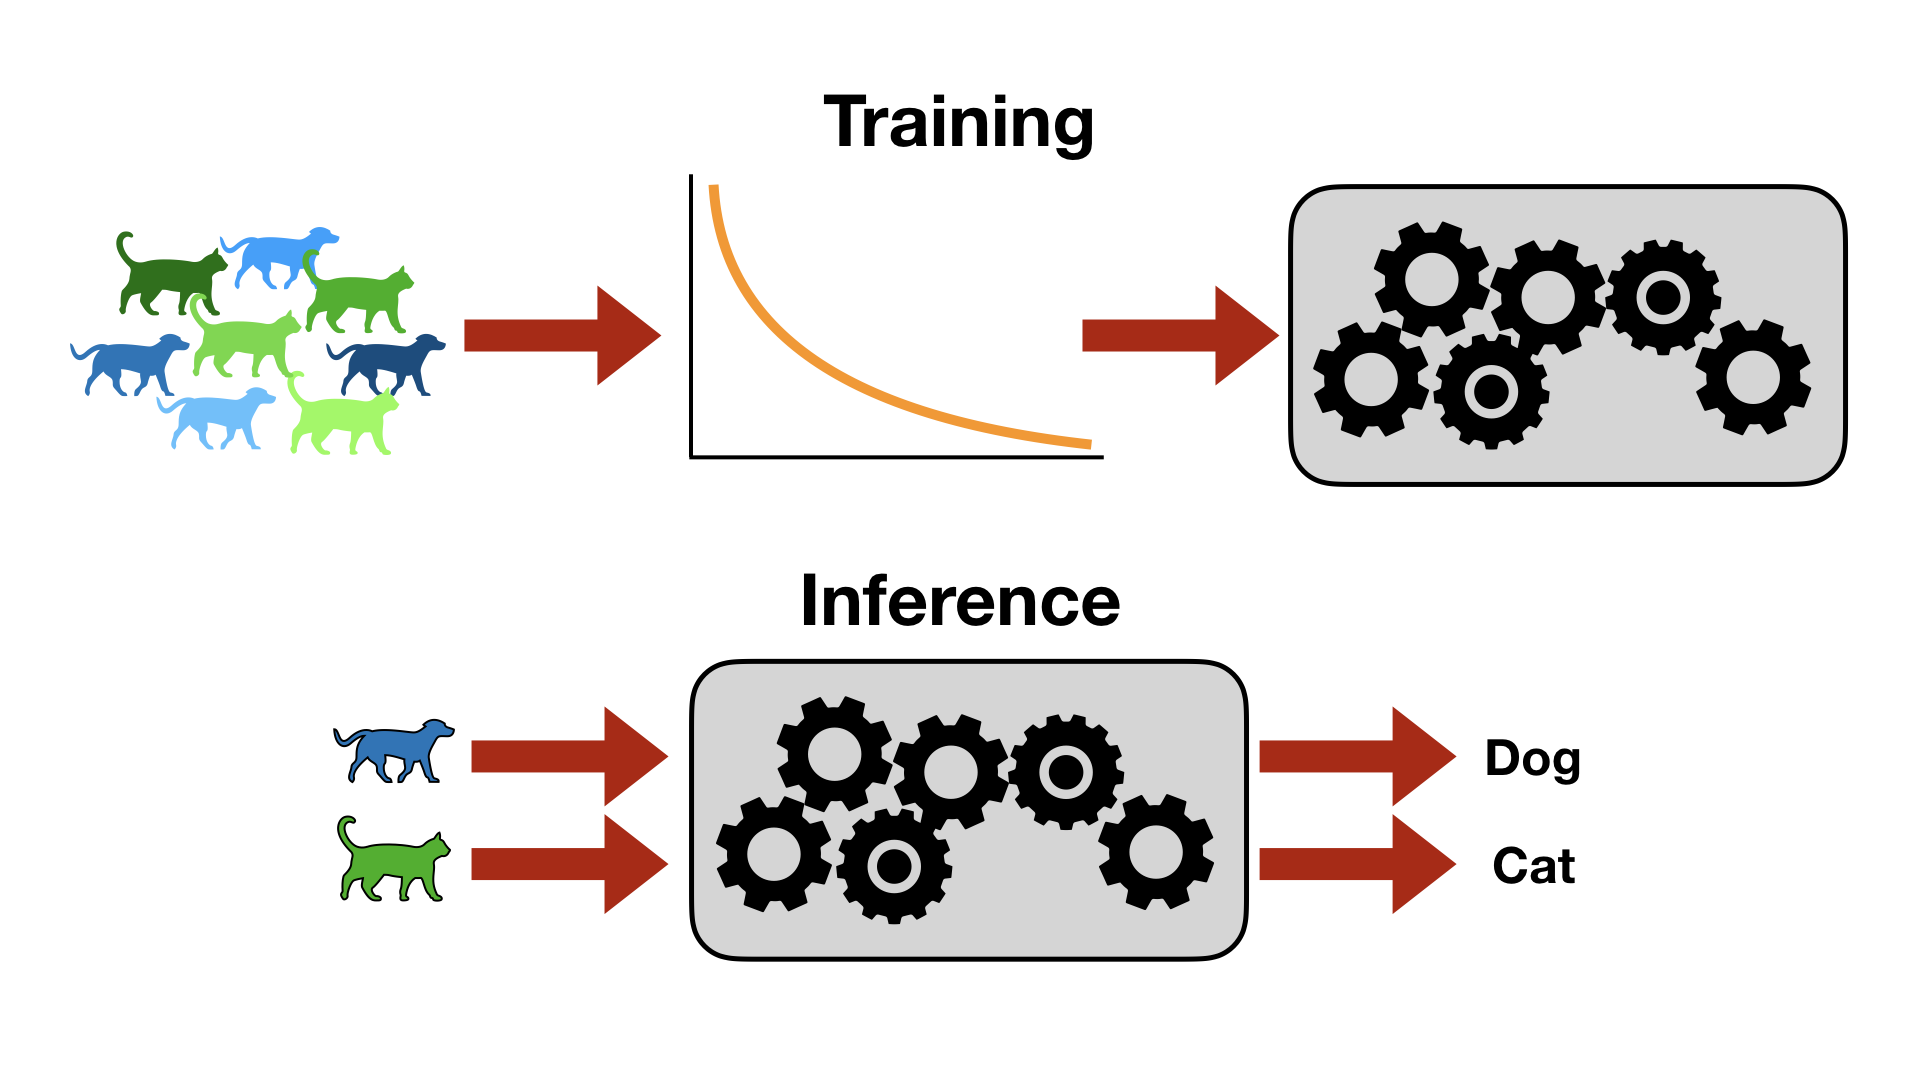
\includegraphics[trim={0 3cm 0 3cm},clip,width=0.95\textwidth]{diss/1_intro/figs/dl.png}
    \caption[Modern machine learning pipelines]{Machine learning training and inference visualization.}
    \label{fig:dl}
\end{figure}

% \textit{Explainability} can be seen as identifying important features of the input, as well as parts of the model (parameters) that ``light up`` for that input. \textit{Fairness} can be evaluated via measures over subsets of the data that correspond to specific groups. 

\begin{mdframed}[style=MyFrame]
\em 
\textbf{This thesis} focuses its main efforts on identifying these important subsets of model, feature, and sample space, to enable answering questions necessary for mainstream adoption of machine learning methods.
\end{mdframed}

% In this dissertation, we explore the sizes of these models, samples, and datasets, and 
% analyze under what situations 
% a smaller \textit{subset} of them may be sufficient or important
% for questions that run parallel to standard performance and accuracy measures.

Let us step a bit deeper into a basic illustrative example. In order to ease understanding, we can first begin with a basic formulation of learning methods, from which the questions above can take specific forms. 
Learning methods typically  try to identify a function mapping (model) that is able to complete a specific task at some high level of profficiency.
% In Figure~\ref{fig:dl}, a model is trained using examples of classification task (top), in order to accurately predict the class of a newly provided input (bottom).
% \begin{figure}
%     \centering
%     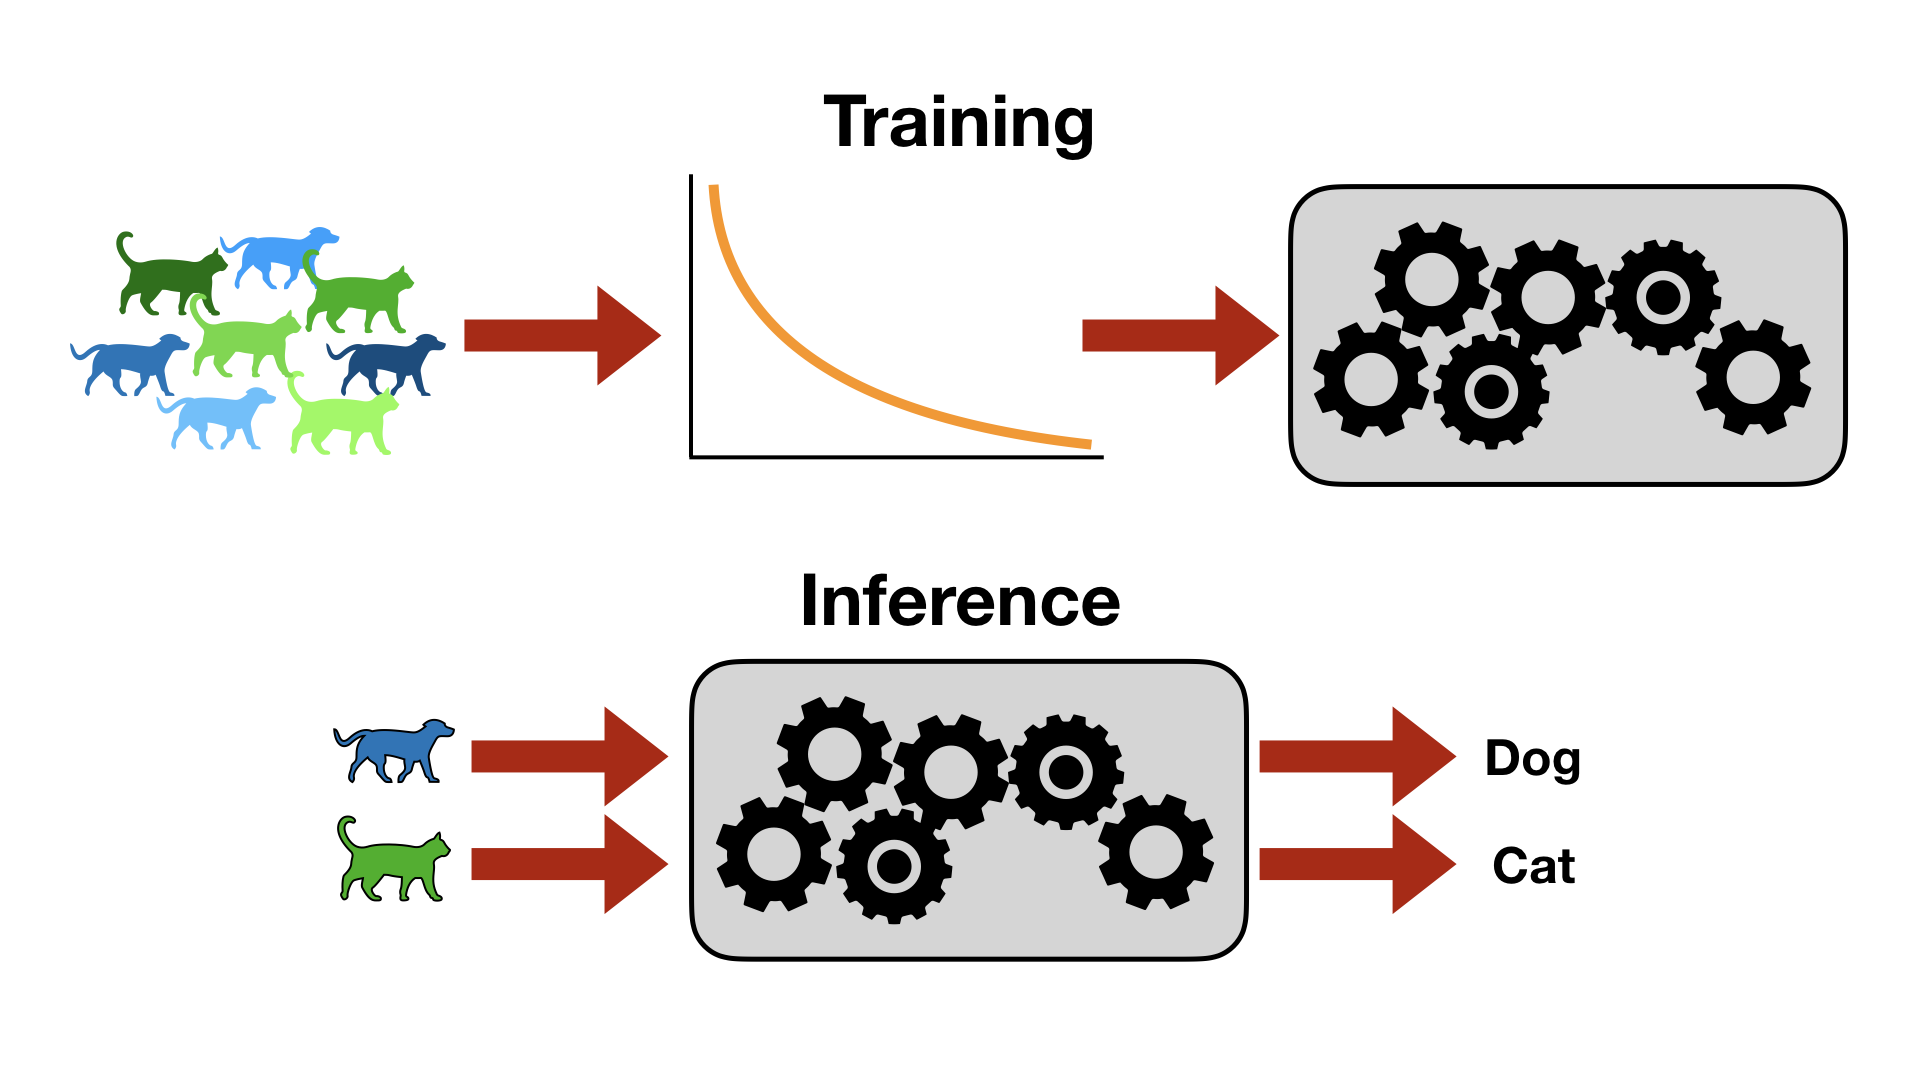
\includegraphics[trim={0 3cm 0 3cm},clip,width=0.95\textwidth]{diss/1_intro/figs/dl.png}
%     \caption[Modern machine learning pipelines]{Machine learning training and inference visualization.}
%     \label{fig:dl}
% \end{figure}
Say we have some dataset comprising of sample pairs $(x,y)$, where we wish to predict $y$ from $x$.
Our prediction, say $\hat{y}$, might be the output of some unknown function $f$ that we attempt to learn from training data. 
Let our approximation to this function be $\hat{y}:=\hat{f}(x)$.
This can take many forms, 
based on assumptions and prior information we may have on the relationships among the data. 
Consider the simple \textit{linear} case,
where we want to learn some parameter $w$ such that $y = w\cdot x$. 
Given $n$ sample pairs $(x_i,y_i)$ indexed by $i$, traditional statistics and optimization literature yield the following \textit{least squares} problem formulation, where we want to minimize the ``squared error'' between the observed values $y_i$ and the predicted $\hat{y}_i:= w\cdot x_i$:
\begin{align}\label{eq:lq}
\hat{f}:=\hat{w} = \mathop{\arg\min}_{w} \sum_{i=1}^n (y_i - w\cdot x_i)^2
\end{align}
This formulation expands without much change to a multi-dimensional form of the input $x$ and respectively, $w$: the canonical case where a number of features, or \textit{covariates} (e.g., symptoms), are used together to predict the outcome (e.g., diagnosis). 
If we are interested in which features of $x$ are important, we can look at the relative values of the learned ``weights'' $w$. In this simple setting, the importance of a feature (say $x^j$) can be exactly determined by the importance of the parameter ($w^j$).
A weight value far from zero may indicate that corresponding feature is important for diagnosis.
% If instead we are interested in which samples are most important, we can use existing methods for sample reweighting or methods that use standard assumptions to efficiently identify important subsets.

In this case and others, traditional statistical learning methods 
have been studied 
for many decades.
Linear regressors, decision trees, and support vector machines
have all been analyzed under these lenses.
% ,
% and as the modern machine learning community
% has returned to these questions recently,
% so has a renewed interest in their methods of analysis.
New research focuses
particularly on the differences
associated with moving from classical \textit{under-parametrized} models to
modern (deep) \textbf{over-parameterized} models: where
the model size vastly outnumbers the number
of input samples.
% , and may even be comparable to 
% the \textit{entire sample space.}
Methods for estimating the number of samples needed,
the time to learn a particular task,
and the generalization ability 
all require new perspectives in this regime.
While nascent, this research
attempts to fill the gap between
statistical and deep models to enable similar measures of sample influence, feature importance, and model understanding. 

\paragraph{A full picture.}
Let us expand our notation from the example above to consider this more general framing.
Consider a dataset $X:=\{x_i\}_{i=1}^n$ of size $n$ where each data point $x_i$ in the set $X$ is drawn from some underlying distribution over the domain $x_i \sim \cX^d$, 
with domain dimensionality (number of features) $d$.
A model $f$ is fit using a parametrization $\theta \in \Theta$,
with $\Theta$ the space of possible parametrizations (models) with some intrinsic dimension $p$. 
%While all three of these problems are closely related, they require different approaches. 
Generalizing the least squares``error measure'' from Eq.~\eqref{eq:lq} to an arbitrary \textit{loss} $\ell$, we have
\begin{align}\label{eq:learning}
    \hat{f}:=\hat{\theta} = \mathop{\arg\min}_{\theta\in\Theta} \sum_{x \in X} \ell(f_\theta(x_i))
\end{align}
From an analysis perspective, 
we might be interested in any one of 
(a) subsets of input features $\cC \subseteq \cX$ that are important for the downstream task,
(b) associating model subsets $\cP \subseteq \Theta$ with specific inputs or groups of inputs, or 
(c) subsets or subgroups of samples $S \subseteq \{X\}$ that are sufficient or representative of the entire dataset.

Crucially, an uninformed search for a subset is computationally infeasible. For a superset of size $n=|X|$, The set of all subsets is the power set, with a size of $2^{n}$! If an identification procedure requires looking over all of these and choosing a ``best'' one by some metric, the procedure will be limited to very small supersets.
Efficient methods have been developed in each of the three contexts above to avoid this exponential search.

\begin{figure}
    \centering
    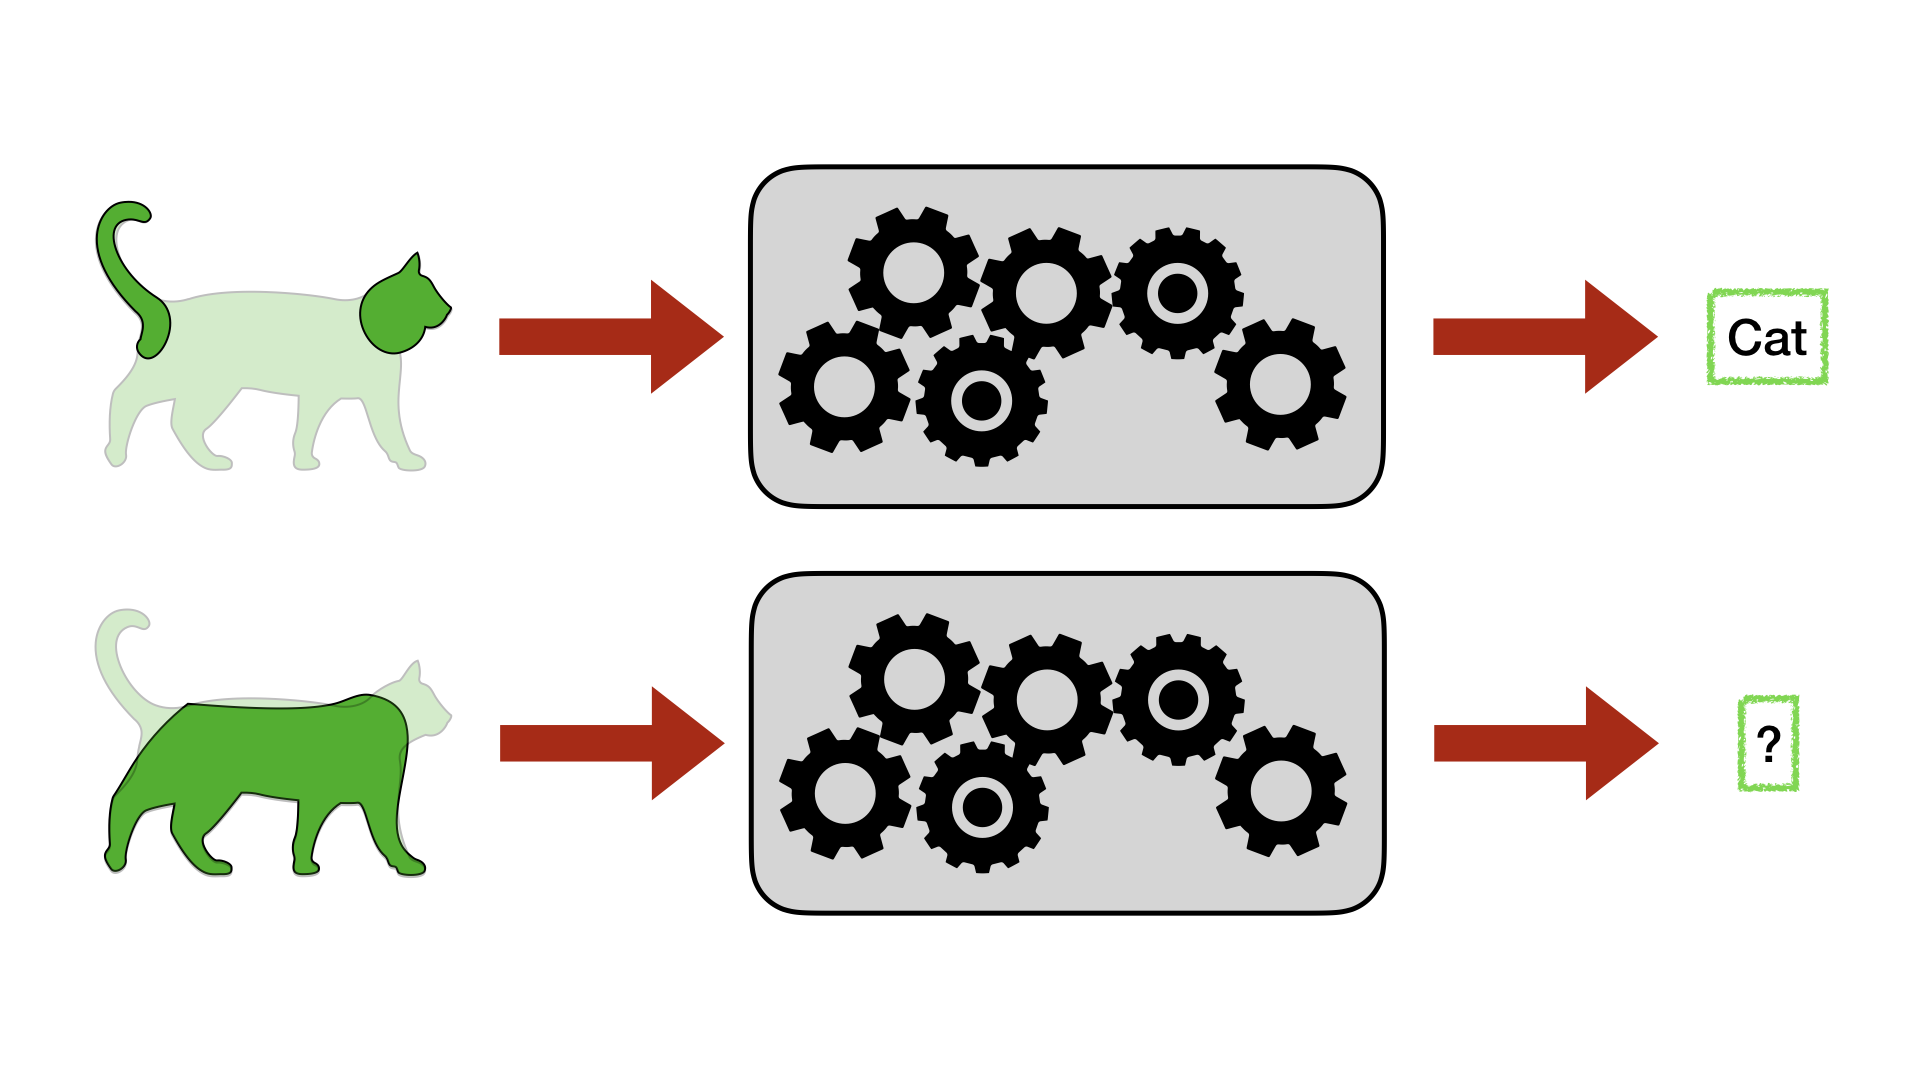
\includegraphics[trim={0 3cm 0 3cm},clip,width=0.9\textwidth]{diss/1_intro/figs/feat_select.png}
    \caption[Visualization of feature selection]{An example of identifying specific features important to the learning task.}
    \label{fig:feat_select}
\end{figure}
\paragraph{Feature Selection.} 
With more complex models $f$ compared to the linear case above, newer ``black-box'' methods have been developed for identifying important features. From the more pure statistics side, scan statistics~\citep{scanstat,scanstatlrt} allow for a structured ``scanning'' over the input space, skipping subsets unlikely to provide additional information for the measure of interest.
Further on the deep learning side, adaptations of sensitivity analysis, via noise addition and perturbations have found success~\citep{yeung2010sensitivity,zhang2015sensitivity}, alongside activation mapping~\citep{cam,selvaraju2017grad}.
These methods typically generate an analagous ``weighting'' over the input space, identifying features most salient for the specific task (Figure~\ref{fig:feat_select}).

\begin{figure}
    \centering
    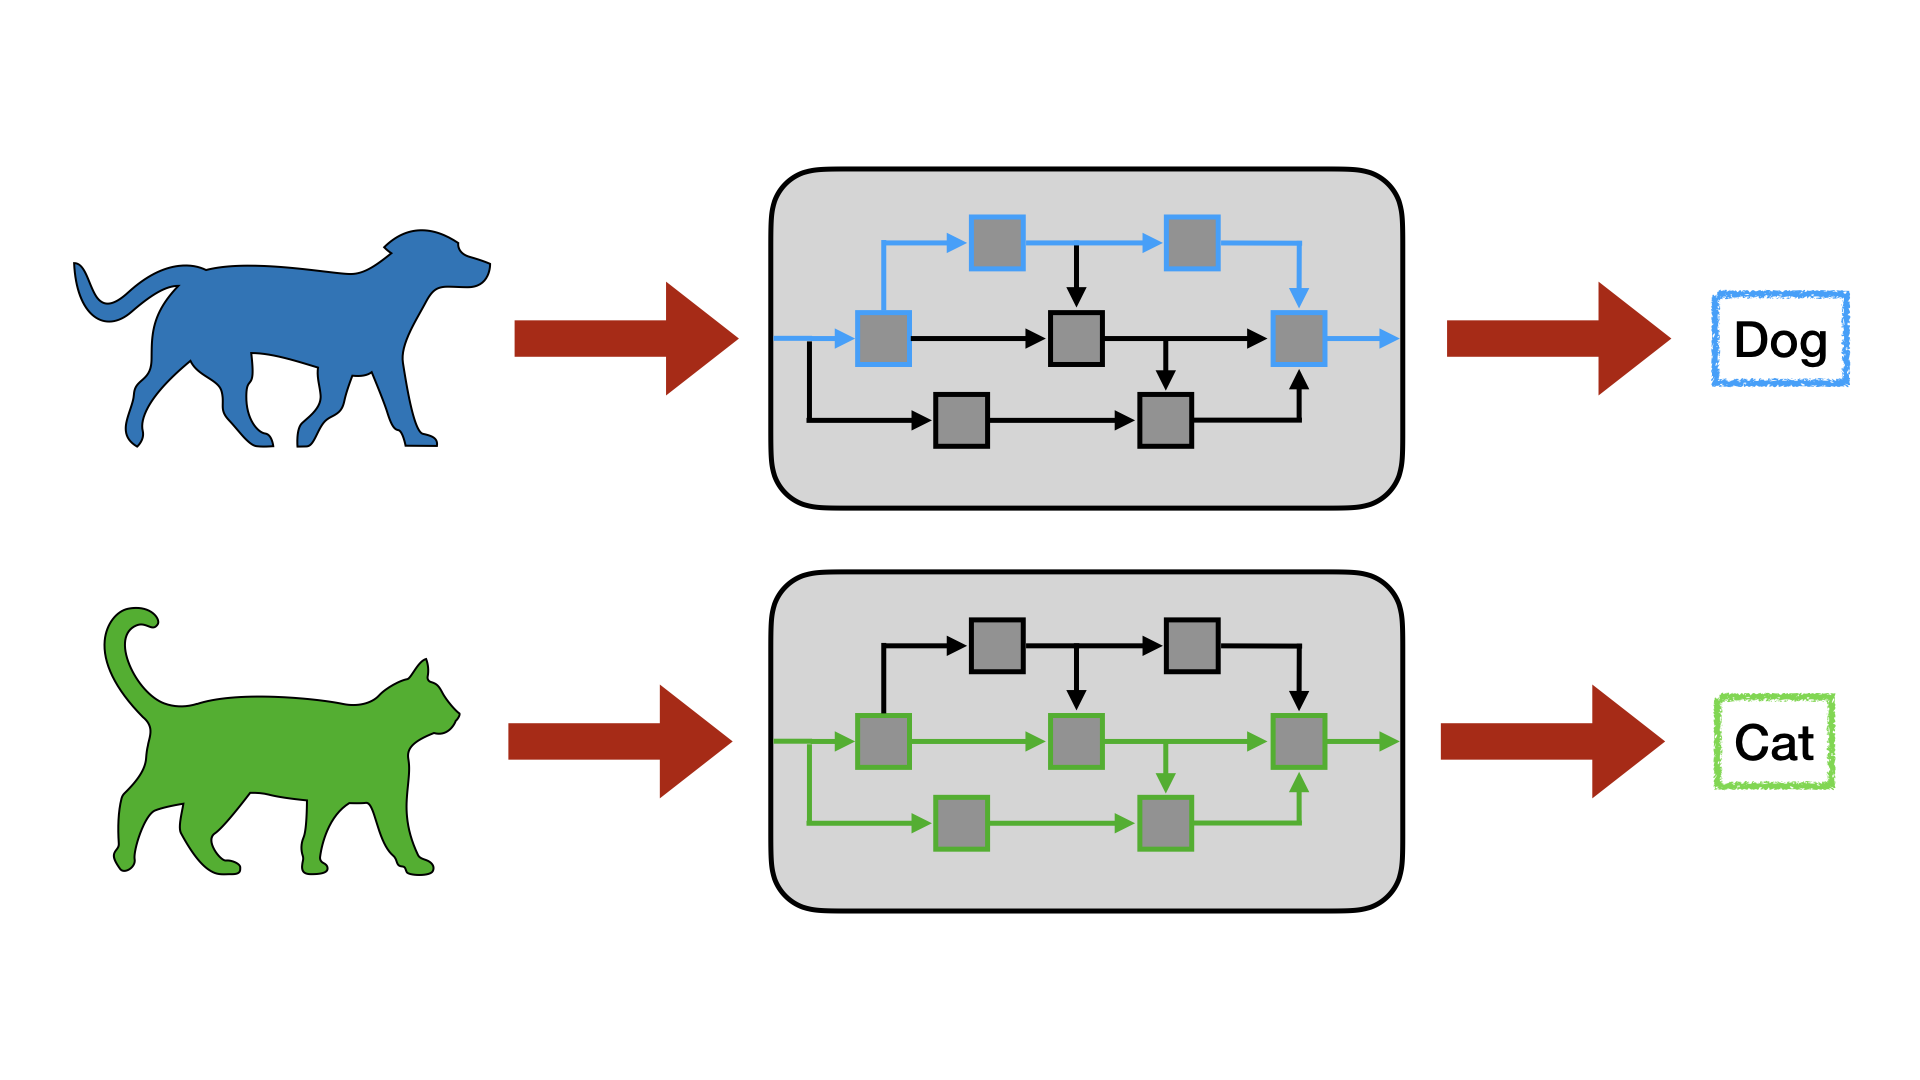
\includegraphics[trim={0 3cm 0 3cm},clip,width=0.9\textwidth]{diss/1_intro/figs/param_select.png}
    \caption[Visualization of parameter selection]{An example of identifying specific parameters important to the learning task.}
    \label{fig:param_select}
\end{figure}
\paragraph{Parameter Selection.} 
Selection in the model space generally takes two forms. First, as a prior, restriction, or assumption over the model space, and second, as a post-hoc method for an ``explainable'' proxy.
Regularization, sparsity, and gating methods are often used independent of the type or size of the model, to encourage the solution to fall within a specific region of the model space.
% In non-deep settings these methods come with strong theoretical guarantees. 
The theoretical underpinnings of these methods in deep learning are still being actively researched~\citep{hardt2016train,jacot2018neural,neyshabur2014search}, but the methods have nonetheless been effective in practice. 
On the post-hoc side, of particular interest are the parameters relevant to specific regions of the input space \textit{after} training (Figure~\ref{fig:param_select}). Here, recent analysis of deployed networks has shown this to be true~\citep{bau2017network,fong2018net2vec}, and current work continues to explore these network regions to aid in interpretability and explainability.

\paragraph{Sample Selection.} Many methods have been developed for outlier detection within training or testing sets~\citep{huang2020feature,ren2019likelihood} \textit{after} training, as well as methods for understanding sample influence~\citep{koh2017understanding,golatkar2020eternal,huang2020feature} . ``In-the-loop'' methods for accounting for ``outlierness'' behave similarly to accounting for group or individual fairness while training~\cite{mehrabi2021survey}. Unfortunately, once samples are identified in some manner, post-hoc adjustments to a trained model are generally very difficult. Recent work has focused on ``unlearning'', or removing a sample's influence on a model without retraining. If specific samples can be uniquely identified, performance and privacy reasons may require these specific interventions to reduce the ``influence'' of that sample subset.
\begin{figure}
    \centering
    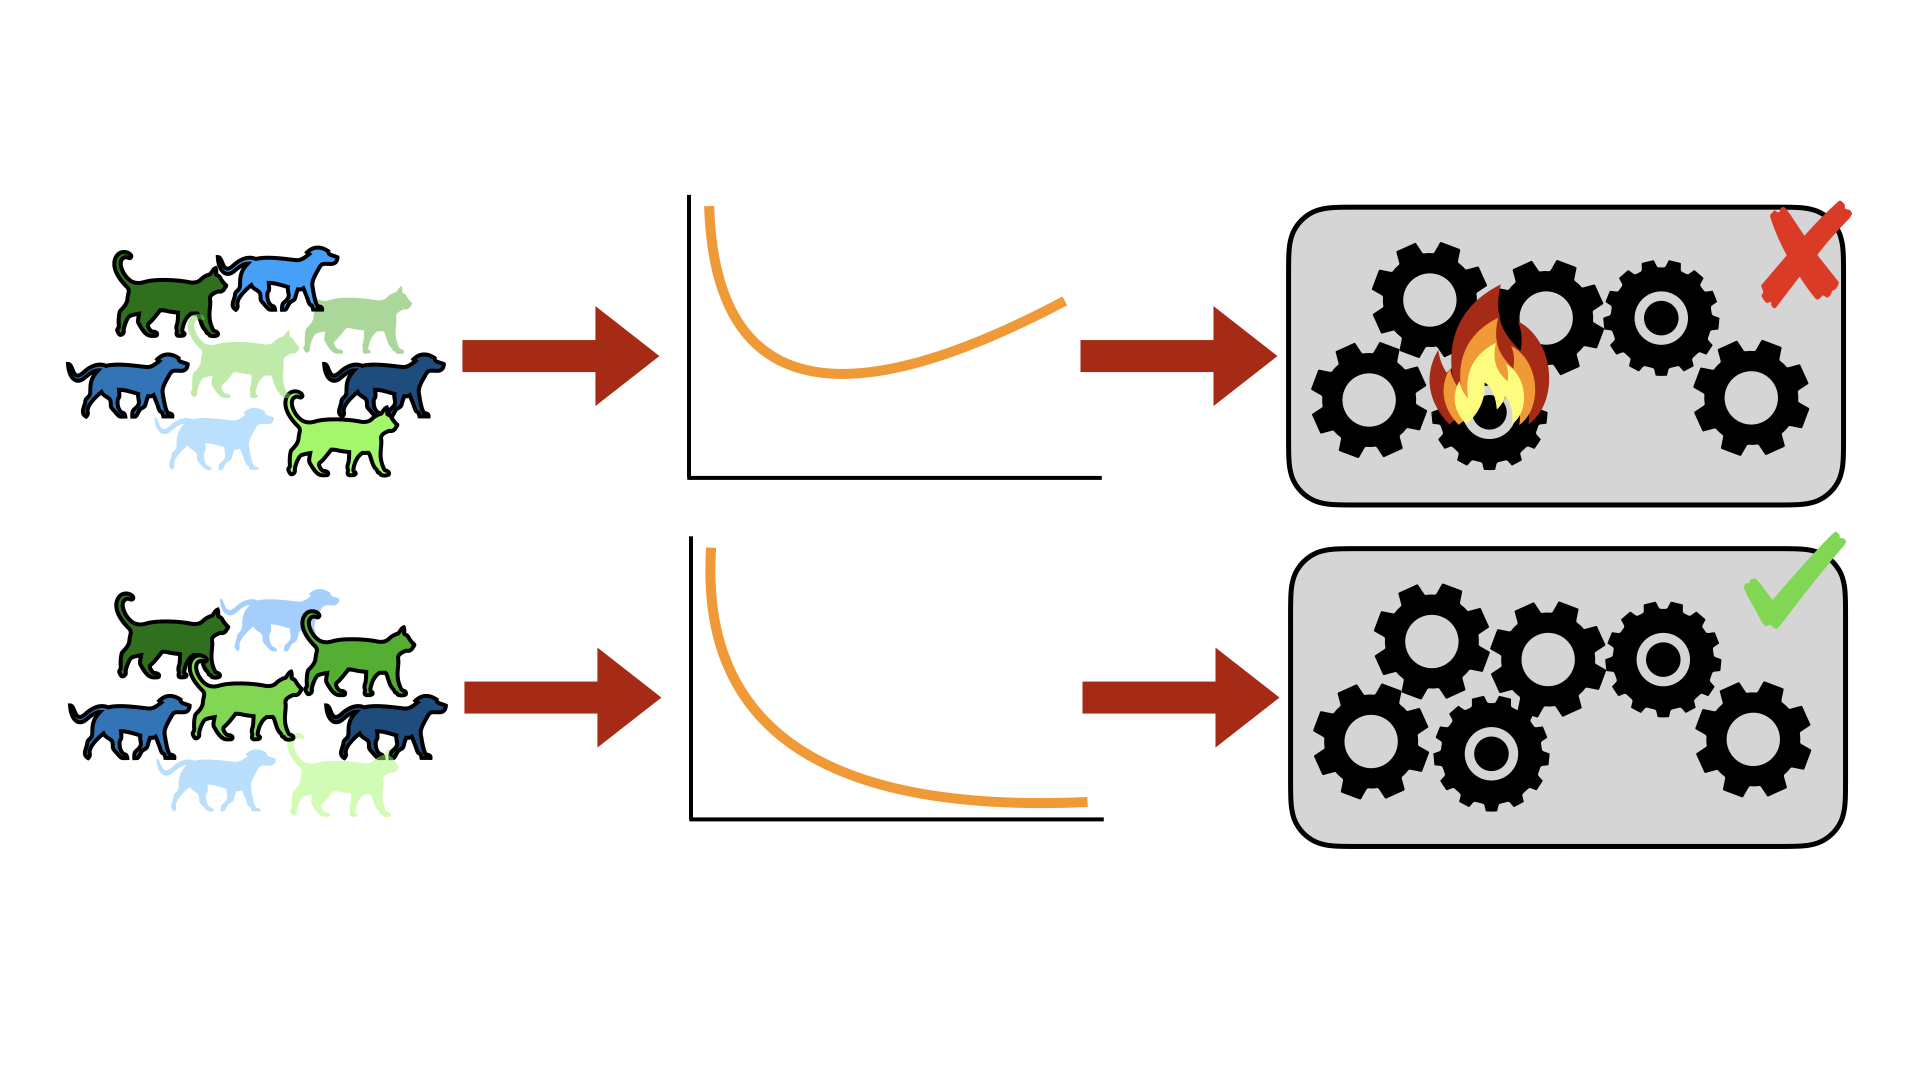
\includegraphics[trim={0 4.5cm 0 4cm},clip,width=0.9\textwidth]{diss/1_intro/figs/sample_select.png}
    \caption[Visualization of sample selection]{An example of identifying specific samples important to the learning task.}
    \label{fig:sample_select}
\end{figure}


\begin{mdframed}[style=MyFrame]
\textbf{ Thesis Goal: }
\em Identify, construct, and evaluate methods for \textbf{efficient} subset identification in modern machine learning feature, model, and input spaces.
\end{mdframed}

\section{A Few Motivating Examples}
Consider a traditional machine learning classification task in which we would like to predict whether an individual has a specific disease condition based on a medical resonance image (MRI) scan of their brain. Our input feature $x$ may consist of a 3D-array of values in $\RR^{\cI\times \cJ\times \cK}$ measuring some intensity of the imaging modality at each voxel, indexed by a tuple $(i,j,k) \in (\cI,\cJ,\cK)$.
Our outcome variable $y$ may simply be a binary label of whether the input scan has been labeled by a radiologist as one demonstrating typical disease characteristics.
Using an off the shelf 3D convolutional neural network with adjustments to match our input size, we can very quickly set up and train a system to predict disease presence with a high degree of accuracy.

\paragraph{Example 1.}
With a prediction for a specific scan, or predictions over a number of scans, we might be interested in identifying which regions of the brain are most important for diagnosis. These regions, $R \subset \cR:=\RR^{x\times y\times z}$, can be specific groups of pixels in the image that may correspond to known functional networks. Methods such as attention and class activation maps may work here, but there are a few issues. The number of samples available to learn a model is very small compared to the both the dimension of the input and the number of parameters in the model, i.e., $n \ll p$ and $n \ll d$. Thus it is very easy to overfit, and for areas of interest to be associated with intricacies of particular input data rather than true, real differences defined by the disease.

Furthermore, recent medical imaging studies have moved past simple difference detection: trends over time, and the ability to predict {\em future} disease development have by far become the setting of most interest.
Given an image of a healthy individual, is it possible to predict what their scan, or their future disease diagnosis, may be up to 10, 20, or more years in the future?
If a number of scans have been collected over some timeframe, can the \textit{trajectory} of the individuals' development be extrapolated to estimate progression?
As traditional models extended for temporal analysis grow in both size and complexity,
a number of subproblems explicitly related to model and input subspaces arise. In this thesis we address two such problems: \textbf{statistically rigorous identification of temporally evolving subsets}, and \textbf{characterizations of deep models that enable efficient training of recurrent models with large scale time-varying data}.
    
\paragraph{Example 2.}
With the rapid growth of AI and machine learning applications has come valid concerns regarding both guarantees of privacy.
Recent technology legislation has made the importance clear in all aspects of data use,
and particular projects and groups have demonstrated that machine learning is not independent of
this need \citep{Exposing}.
A new issue raised within this intersection is the ``right to be forgotten".
If a model has been trained with a particular users' data, 
they should have some recourse or right
to both remove their data from the training set,
and also know that the model has not learned from their data.
On the surface, this poses a significant problem for model builders
and organizations that spend large amounts
of time and resources in 
training deep learning models.

In the medical imaging example above this is especially important: with fewer samples it is more likely that information about any particular one could ``leak'', and the model's performance may degrade significantly as a relatively large percentage of it's training data is removed.
Thus tailored methods must be developed to ensure both privacy and performance, without requiring full retraining.
As we will see, 
\textbf{identification of model parameter subsets}
that are particularly important
for a particular sample's influence
in a model enables \textit{efficient machine unlearning}.

\paragraph{Example 3.}
From an alternative perspective, we may want to identify specific samples rather than have them specified a priori.
Traditionally a rigorous area of study under classical statistics, outlier detection and accounting have become a subfocus for many within the machine learning community as well \citep{golatkar2020eternal,golatkar2020forgetting,huang2020feature,ren2019likelihood}.
While subgroups of input samples may be outliers, it is more often the case that they represent known heterogeneity within the data. 
These differences may be marked using 
group information known a priori, and 
most learning tasks aim to learn tasks
in a \textit{subgroup-independent} manner.
In our disease prediction model above,
these groups could simply be stratified by the type of scanner used to acquire the image, but it could also
be a systematic difference correlated with some protected attribute. {\color{red} sentence about original brain atlas for registration being eurocentric}
This can directly lead to disparate performance and results on \textit{all} individuals outside of that group.
Optimization and regularization methods with this focus come under the umbrella of model fairness.
However, many existing methods do not scale well to larger models or as the number of subgroups grows, as is often the case when intersections of protected classes must be considered. Here we identify and construct a particular solution for \textbf{groupwise fairness that enables efficient in the loop fairness regularization}.

% What features are most important for prediction?
% Which samples were most important for my training?
% Can we understand when a model is certain or uncertain about its output?
% Are there layers in my network that have learned a particular subtask?
% Questions of robustness, bias, influence, fairness, and importance have become central questions to contemporary machine learning research \citep{doshi2017towards,mehrabi2021survey,amodei2016concrete}.
% machine learning, etc.

% Feature selection in the case of
% typical regression or classification 
% takes some form of learning parameters $\theta$ that allow for $\hat{y} = f_\theta(x)$ to be close to the true outcome of interest $y$.
% While forms of data $X := (x,y)$ may simply be continuous and real-valued, modern machine learning has greatly expanded formulations of the classical learning problem to include a wide variety of structured learning problems~\citep{nowozin2011structured}. 
% Consider the case when a high-dimensional input is used to predict an output with a highly-parametrized model. 
% Once learned, obvious questions arise as discussed above: are there specific low-dimensional spaces in either the input or the model space that are most important or necessary for the global learning problem of interest? Are there specific subspaces associated with particular subproblems of the global problem?
% The machine learning literature has come up with a number of ways to identify analogs of these spaces, 
% including extensions of sensitivity analysis to deep learning~\citep{yeung2010sensitivity,zhang2015sensitivity}, and constructing and identifying nonzero model subsets via particular model choices such as activations~\citep{selvaraju2017grad} and regularizers.
% In classical settings these are well understood: decision trees naturally provide ease of interpretibility via the information used to choose splits, and both linear and kernel support vector machines have been analyzed to provide for measures of sample importance via distances to the margin as well as feature importance via weights defining the learned hyperplane~\citep{Mitchell97}.
% Attention and saliency maps have emerged as popular new methods,
% given their ease of implementation and interpretation~\citep{sutskever2014sequence,vaswani2017attention,selvaraju2017grad}.
% By learning dimensions of a given input that are particularly important, either in a hard (binary) or soft (continuous weighting) manner, model builders are better able to understand and interpret what a model has learnt.
% The specific ideas of attention notwithstanding, many of these existing methods are far removed from traditional hypothesis testing frameworks.
% While some work has begun in this direction~\citep{tansey2018black},
% there remains a gap in direct identification of subsets and structures in these spaces that can be defined in statistically rigorous manners.

% \begin{figure}
%     \centering
%     \includegraphics[width=0.5\textwidth]{example-image-a}
%     \caption[A simple subset selection example]{\color{red} Identifying and selecting in MRIs, subset, sample, model ID.}
% \end{figure}

% \paragraph{A specific example.} 

% ------------------------------------------

% below here will be moved and arranged with the "selection" sections and here if relevant

% ------------------------------------------

% While attention can be directly applied to the network in order to identify ``hotspots" in the input space relating to the learned classification task, 
% given the high-dimensional nature of the input
% and the relatively small sample size 
% associated with medical imaging data, 
% it is very likely that an area of interest identified
% may be an intricacy of the training samples used rather than truly a region of disease signal.
% Class activation maps (CAMs) may be unclear, and can often associate with image artifacts unrelated to the scientific task~\citep{adebayo2018sanity}.
% Methods of generalization may help to increase confidence in identified regions, but statistical guarantees often remain out of reach.

% Furthermore, most recent problems associated with medical data have moved past simple difference detection: trends over time, and the ability to predict {\em future} disease development has by far become the setting of most interest.
% Given an image of a healthy individual, is it possible to predict what their scan, or their future disease diagnosis, may be up to 10, 20, or more years in the future?
% If a number of scans have been collected over some timeframe, can the \textit{trajectory} of the individuals' development be extrapolated to estimate progression?
% As traditional models extended for temporal analysis grow in both size and complexity,
% a number of subproblems explicitly related to model and input subspaces arise. Here we address two such problems: \textbf{statistically rigorous identification of temporally evolving subsets}, and \textbf{characterizations of deep models that enable efficient training of recurrent models with large scale time-varying data}.

% A sample's particular influence on model parameters aside, the identification of influential samples or subsets of samples more generally is of independent interest. 
% Traditionally a rigorous area of study under classical statistics, outlier detection and accounting have become a subfocus for many within the machine learning community as well \citep{golatkar2020eternal,golatkar2020forgetting,huang2020feature,ren2019likelihood}.
% While subgroups of input samples may be outliers, it is more often the case that they represent known heterogeneity within the data. 
% These differences are typically marked using 
% group information known a priori, and 
% most learning tasks aim to learn tasks
% in a \textit{subgroup-independent} manner.
% Optimization and regularization methods with this focus come under the umbrella of model fairness, and instead of identifying and boosting independences within the model or data, we aim to minimize them.
% However, many existing methods do not scale well as the number of subgroups grows, as is often the case when intersections of protected classes must be considered. In the sequel we identify and construct a particular solution for \textbf{groupwise fairness that enables efficient in the loop fairness regularization}.

\begin{mdframed}[style=MyFrame]
\em 
Here we focus our effort on identifying these important subsets of model, feature, and sample space for feature association, model size reduction, model unlearning, and, fairness. Specifically, taking advantage of both existing statistical and geometric methods, we develop new methods for localizing subsets in a range of settings from hypothesis testing to deep learning.
\end{mdframed}

\section{Thesis Scope and Contributions}

We explore the intersections of classical statistical and geometric constructions with modern machine learning methods. 
Figure~\ref{fig:scope} shows the overall scope projected along three axes: feature, parameter, and sample spaces.
Below we briefly introduce the main problems studied in this thesis.
\begin{figure}[!ht]
    \centering
    % \includegraphics[width=0.99\linewidth]{scope.pdf}
    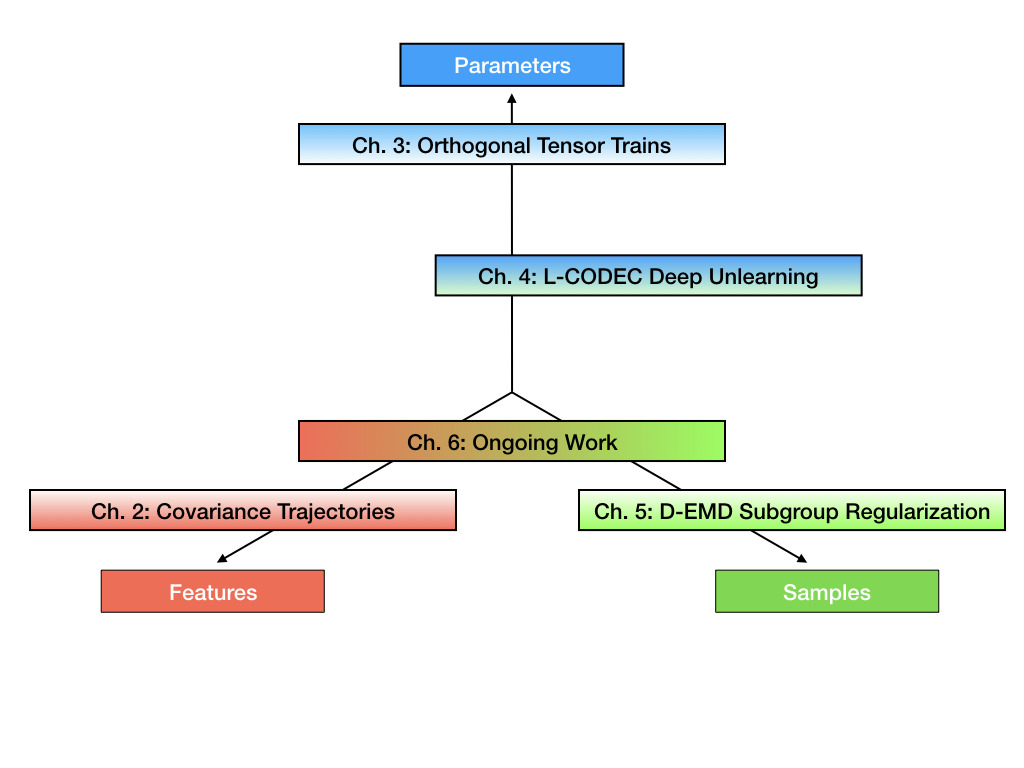
\includegraphics[width=0.95\linewidth]{diss/1_intro/figs/thesis_scope.png}
    \caption[Thesis Scope]{Thesis scope, projected over three representative axes. {\color{red} update chapter numbers shift by 1}}
    \label{fig:scope}
\end{figure}

\subsection{Second-Order Modeling and Group Difference Analysis over Time}

Recent results in coupled or temporal graphical models offer schemes for estimating the relationship structure 
between features when the data come from
related (but distinct) longitudinal sources. A novel application of these ideas is for analyzing group-level differences, i.e., in identifying if {\em trends} of estimated objects (e.g., 
covariance or precision matrices) are different across disparate conditions (e.g., gender or disease). Often, poor effect sizes make detecting the \textit{differential} signal 
over the {\em full} set of features difficult: for example, 
dependencies between only a {\em subset of features} may manifest differently across groups.
We first suggest
a parametric model 
for estimating trends in the space of $\SPD$ matrices as a function of one or more covariates.
We will then generalize scan statistics to graph structures, 
to search over distinct subsets of features (graph partitions) whose temporal dependency structure may show statistically 
significant group-wise differences.
We will theoretically analyze the Family Wise Error Rate (FWER) and bounds on Type 1 and Type 2 error. 
On a cohort of individuals with risk factors for Alzheimer's disease (but otherwise cognitively healthy), 
we 
find scientifically interesting 
group differences where the default analysis, 
i.e., models estimated on the full set of features, do not survive reasonable 
significance thresholds. 
% Preliminary work on this was published in \citep{covtraj}.


\subsection{Efficient Tensor Representations for Feasible Temporal Deep Learning}

Modern deep networks have proven to be very effective for analyzing real world images.
However, their application in medical imaging is still in its early stages,
primarily due to the large dimension of three-dimensional images, requiring enormous convolutional or fully connected layers --
if we treat an image (and not image patches) as a sample. 
These issues only compound when the focus moves towards longitudinal analysis
through recurrent structures, and when a point estimate of model parameters is insufficient 
in scientific applications where a reliability measure is necessary.
Using insights from differential geometry, 
we will adapt 
the tensor train decomposition to construct networks
with significantly fewer parameters,
allowing us to train powerful recurrent networks on whole brain image volumes. 
We analyze 
the \textit{orthogonal tensor train},
and demonstrate its ability to express a standard network layer both theoretically and empirically.
We 
demonstrate its ability to 
effectively reconstruct whole brain volumes
with faster convergence and stronger confidence intervals
compared to the standard tensor train decomposition. 
We provide code and show experiments on the ADNI dataset
using image sequences to regress on a cognition related outcome.
% Preliminary work on this was published in \citep{ott}.

\subsection{Practical Unlearning via Large-Scale Conditional Independence Testing}

%With AI systems extensively using personal %data for model training, 
Recent legislation has
led to interest in {\em machine unlearning}, i.e., removing specific training samples from a {\em predictive} model as if they never existed in the training dataset. 
Unlearning may also be required due to  corrupted/adversarial data or simply a user's updated privacy requirement.
For models which require no training ($k$-NN), 
simply deleting the closest original sample can be effective. 
%However, it is not clear how such approaches can be used to unlearn 
%models that contain rich information learned from the original data.
But this idea is inapplicable to models which learn richer 
representations.
%from data. 
%Recently, optimization-based unlearning estimators have been proposed, but 5their 
Recent ideas leveraging optimization-based updates
scale poorly with the model dimension $d$,  
due to 
inverting the Hessian of the loss function. %with an overall cost of $O(d^3)$ 
%is prohibitive.
We describe
a variant of a new conditional independence coefficient, 
L-CODEC, to identify a subset of the model parameters with the most semantic overlap on an individual sample level. 
Our approach completely avoids the need to invert a (possibly) huge matrix. 
By utilizing a Markov blanket selection, 
we find
that L-CODEC is also suitable for deep unlearning,
as well as other applications in vision.
Compared to alternatives, L-CODEC makes approximate unlearning possible 
in settings that would otherwise be infeasible, 
including vision models used for face recognition, 
person re-identification 
and NLP models that may require unlearning samples identified for exclusion.
% Preliminary work on this will appear in \citep{lcodec}.


\subsection{Reducing Subgroup Fairness via High Dimensional Earth Mover's Distances}

Optimal transport has recently emerged as a useful tool for machine learning through its connections with geometry, statistical machine learning, and through practical algorithms. Existing methods that leverage optimal transport often  regularize using  a Wasserstein metric or by computing barycenters, for example. %which are effective when distributions are continuous and known, or when measures of interest are discrete.
% Our formulation allows for a discretization of continuous measures that drop in directly to classical  formulations of the Earth Mover's Distance. 
We leverage optimal transport, except that we take advantage of a recently-introduced algorithm that computes a generalized earth mover's distance.
Not only is this algorithm computationally cheaper to compute compared to existing barycentric measures, but our method has the additional  advantage that gradients used for backpropagation can be directly read off of the forward pass computation, which leads to substantially faster model training.
We provide technical details about this new regularization term and its properties, 
and 
experimental demonstrations of improved training speed over existing Wasserstein-style methods.

{\color{red}
\subsection{Understanding Latent Spaces via Conditional Independences}

The final chapter of this thesis applies some of the tools developed above in the analysis of latent spaces in recent large scale models.
% In these studies, 
% we aim to identify conditionally independent features and subjects that are particularly important to the prediction and estimation of
% key disease outcomes,
% as a function of a number 
% of demographic, neuropsychological,
% genetic,
% and imaging data collected as 
% part of an ongoing consortium 
% to understand the progression
% of Alzheimer's disease in younger, 
% asymptomatic populations.
% In what follows we present
% exploratory analysis
% on a small, easily 
% digestible subset of the available data,
% that lays the foundation for
% further analysis.
}
% This work is the most forward looking, and aims to be a stepping stone toward a rigorous 

\section{Outline}
Chapter 2 covers the essential background necessary for the developments presented in the following chapters, including specifics of graphs and hypothesis testing, as well as relevant modern methods for learning and optimization.
In Chapters 3 through 7, we describe four perspectives to address subset identification.
Chapter 3 explores and focuses on the identification of feature subsets varying over time.
In Chapter 4 we describe a method of constraining the parameter space in a particular manner
that enables more efficient large scale neural networks.
Next, Chapter 5 provides a solution to the machine unlearning problem,
enabled through a particular conditional independence parameter selection scheme, vastly reducing network update costs.
Chapter 6 ends with a unique solution to subgroup fairness, 
where we take advantage of an efficient solution to
the $d$-dimensional earth mover's problem
to regularize large models when the number of subgroups can be large.
{\color{red} Chapter 7 describes future work, focused on applying a particular solution from Chapter 5 to understanding relationships among features in latent spaces learned by large generative models.}


%%%%%%%%%%%%% 
% Some old stuff

% Significant progress in the modern development of machine learning has
% been built upon connections and patterns identified across myriad
% interdisciplinary fields of study.
% Up through the mid 2000's, 
% many of these methods were inspired by and interested in 
% highly focused and constrained problems. 
% With a reasonably sized input domain, could a model of roughly equal size be used to
% predict some output?
% Linear regressors, decision trees, and support vector machines were all answers to these questions, with their own
% varying degrees of scaling and complexity.
% These methods necessitated carefully constructed formulations with specific restrictions to the learnable function class,
% enabling straightforward analysis 
% for provable performance guarantees 
% and easy identification of critical training samples and important input features.

% Contemporary machine learning, however, has a vastly different modus operandi. 
% Driven in large part by the exponential growth of available computation via Moore's Law, \textit{deep learning} has fallen squarely in the realm of \textbf{over-parameterized} models.
% With these overparametrizations and computation capacity, the typical learning questions posed as maximizing accuracy or reducing error have largely been addressed for even large scale problems.
% As such, complementary questions have led to subfields focusing on other performance measures, such as robustness, fairness, interpretability, and explainability.
% Many solutions to these questions end up looking back at answers found for the under- or non-parametrized settings.
% While nascent, these approaches 
% attempt to fill the gap between
% statistical and deep models to enable similar measures of sample influence, feature importance, and model analysis. 
% Most notable amongst these newer approaches is that of (Self)-Attention in Neural Networks \citep{sutskever2014sequence,vaswani2017attention}.
% Other proposals 
% end up looking back at the types of analysis typical of those more classical under-parametrized or nonparametrized methods.

% Not limited to previous developments in learning or computation theory, the arguably most valuable contributions toward the exponential reduction in model error can be attributed to influences and intuitions taken
% from biology, psychology, neuroscience, and even XXX \citep{srivastava, etc}.
% Perhaps one explanation as to why this phenomenon exists may be attributed to the way in which deep learning evolved. 
% The classical learning goal of function approximation lends itself nicely to a system which allows for arbitrary complexity via simple changes (e.g., addition of neural network layers). % Foundational works building on the original neural networks particularly have taken advantage of constraining this space of functions to search over: 
% the most seminal case being those of convolutional filters for imaging data. 
% While ``constraints" of this form have helped tremendously in model performance on modern vision and language machine learning tasks (GANs, Recurrent Networks, Residual Layers, Transformers, etc.), the ability to identify \textit{subsets} of important samples, input features, and model parameters has lagged significantly behind the development of these methods.
% Recently larger interest has been taken by the community to understand and interpret models with this view, only after extremely large and opaque models have become ubiquitous.
%This lag directly explains the more recent interest in developing methods for understanding and interpreting large scale machine learning models. % LCODEC
% \chapter{Introduction} \label{chap:intro} 

Modern applications of machine learning in a broad range of industrial and consumer-facing systems have become ubiquitous.
Most interactions with daily technologies now intrinsically involve 
a request to some ``smart`` system in the ``cloud'', 
where those interactions range from
a request for map directions 
to simply loading a webpage.
Neural network models, and the recent advances of deep learning,
have enabled these systems that 
make such applications possible.
These models have achieved
human-level performance on learning tasks
including image classification~\citep{resnet,alexnet}, image segmentation~\citep{segmentation}, video analysis~\citep{zhang2016video}, text understanding and generation~\citep{bert,gpt}, and have slowly begun to solve more fundamental scientific problems such as protein folding~\citep{protein} drug discovery~\citep{drugdisc}, and medical diagnosis~\citep{diag}.
While this performance is largely attributed to model size,
the abundance of high quality training data
has equally contributed to real world performance,
enabling model training over millions of real world samples~\citep{imagenet,laion},
and potentially billions of synthetic samples via environment simulation~\citep{mcts}.

While deployment in some domains (recommender systems, object detection) may benefit almost unconditionally from this vastly expanded capability, rightful hesitancy has limited their widespread use in particular applications where impacts on individuals, people, or environments may be at stake.
These ``last mile'' concerns take a few forms.
% Because a completely accurate model is still out of reach, an important question that needs to be answered is: which inputs or individuals are being given incorrect outcomes, and why?
% maybe a sentence suggesting unlearning/removal
In mission critical applications such as medical diagnosis, 
the impact of an error can be extremely large,
even if a misprediction happens extremely infrequently.
Additionally, large scale model training and architecture search
can require exorbitant amounts of energy producing high emissions,
and their scale can limit market participants
to only large actors with vast existing resources.
The accessibility and effectiveness of these models can also vary significantly based on the training data, and disparate outcomes can be exacerbated by existing social inequity.

While existing human or ``natural'' systems that these models aim to assist are not perfect, 
our real world has developed norms and regulations that 
enable them to function.
A medical diagnosis might require a physician to explain what symptoms led them to that particular conclusion.
Energy metering and carbon taxes may be applied to limit
emissions.
Regulatory satisfaction may require 
analysis proving equal opportunity,
or that specific protected classes
are not used in decision making.
% Specifically, these can include ideas as simple as the Hippocratic Oath and medical malpractice insurance, to asking your doctor what symptoms lead them to a particular diagnosis.
These ideas are difficult to directly translate to automated machine learning systems,
but proxies have been identified that we can build upon.

These norms and regulations answer a number of questions we may also try to pose to our machine learning models.
What is the cost to learn this task?
What led to this particular outcome?
Why is this outcome different from another?
% We will explore how these questions can be formulated concretely. 

If the answer to these questions is negative or unknown,  follow-up questions all take an interesting form:
Can we learn a smaller model with similar performance? 
Can we identify the most important features? 
Which individuals or groups are being treated unfairly, and can we change that?
These questions ask us to identify a \textit{subset} of some relevant set, dependent on setting, and this identification is our focus here.

% Moving specifically to machine learning methods,
Taking a step back, let's take a look at a representative system. Figure~\ref{fig:dl} illustrates a typical learning pipeline. 
A dataset is collected and used to train a model, by minimizing the error over
those samples in the dataset (top).
A ``sample'' can be a single measured value, or it can
be a large, highly structured object with many ``features.''
The model is made up of some ``parameters'' that are 
tuned during training to learn a good predictor over the training dataset.
This model is then used to predict, or \textit{infer}, on new
data seen ``in the wild'' (bottom).
Our questions above are formally asking to identify \textit{subsets of these objects}: is a subset of the model parameters sufficient for learning? Which subset of the features are important for a prediction? Which subset of the dataset exhibit a specific attribute?
\begin{figure}
    \centering
    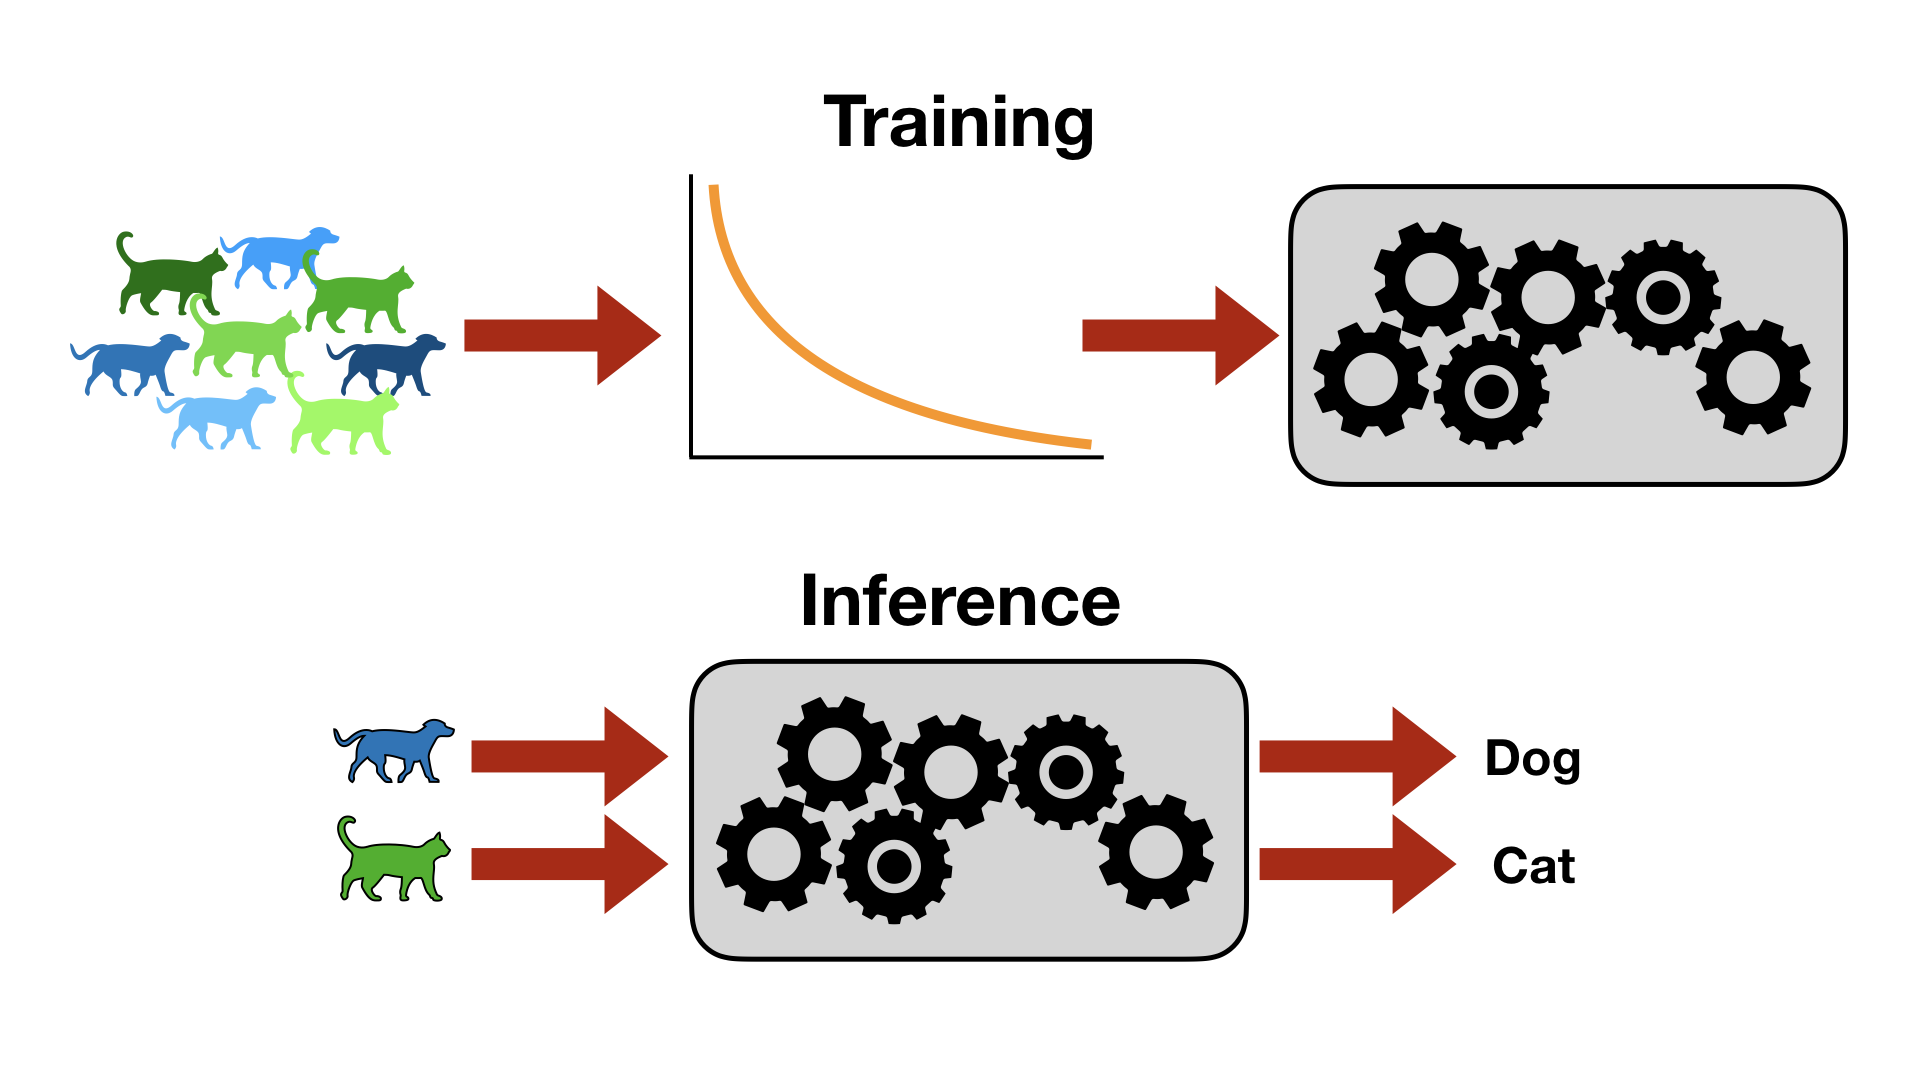
\includegraphics[trim={0 3cm 0 3cm},clip,width=0.95\textwidth]{diss/1_intro/figs/dl.png}
    \caption[Modern machine learning pipelines]{Machine learning training and inference visualization.}
    \label{fig:dl}
\end{figure}

% \textit{Explainability} can be seen as identifying important features of the input, as well as parts of the model (parameters) that ``light up`` for that input. \textit{Fairness} can be evaluated via measures over subsets of the data that correspond to specific groups. 

\begin{mdframed}[style=MyFrame]
\em 
\textbf{This thesis} focuses its main efforts on identifying these important subsets of model, feature, and sample space, to enable answering questions necessary for mainstream adoption of machine learning methods.
\end{mdframed}

% In this dissertation, we explore the sizes of these models, samples, and datasets, and 
% analyze under what situations 
% a smaller \textit{subset} of them may be sufficient or important
% for questions that run parallel to standard performance and accuracy measures.

Let us step a bit deeper into a basic illustrative example. In order to ease understanding, we can first begin with a basic formulation of learning methods, from which the questions above can take specific forms. 
Learning methods typically  try to identify a function mapping (model) that is able to complete a specific task at some high level of profficiency.
% In Figure~\ref{fig:dl}, a model is trained using examples of classification task (top), in order to accurately predict the class of a newly provided input (bottom).
% \begin{figure}
%     \centering
%     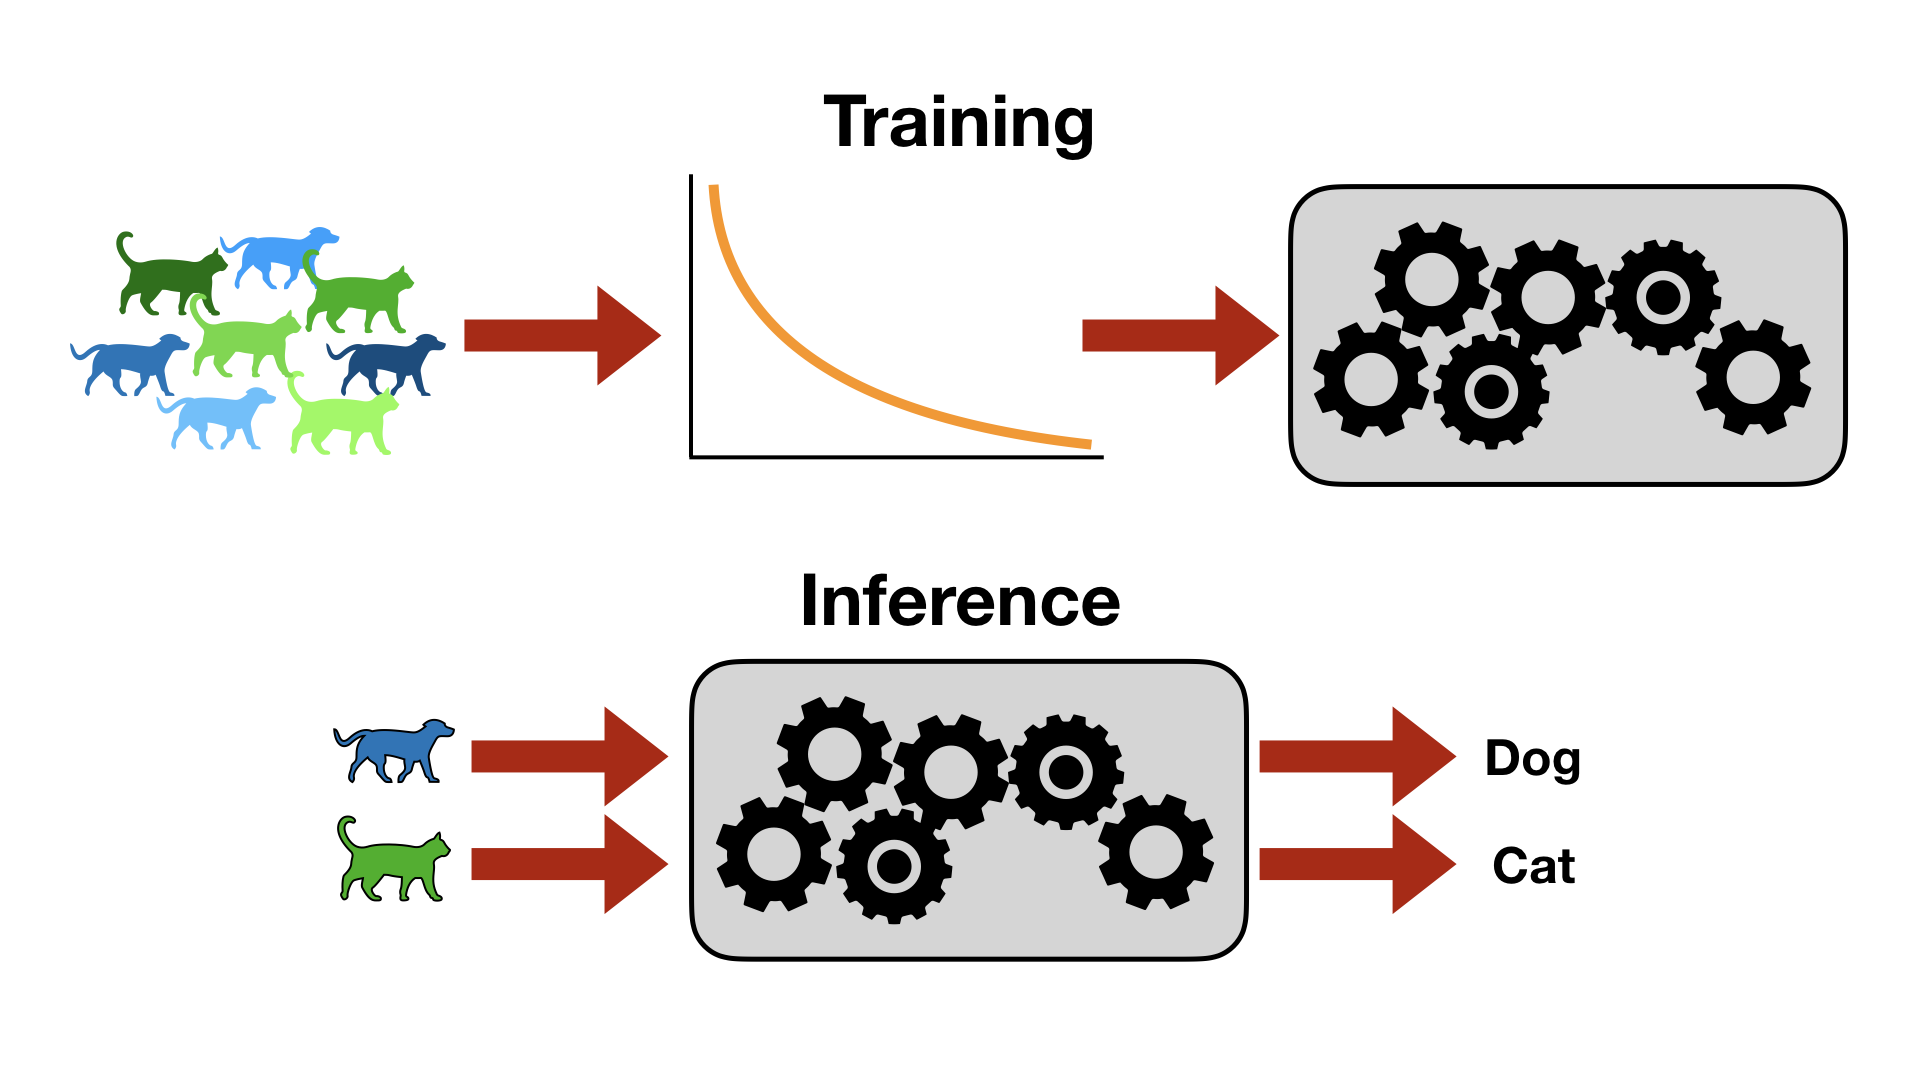
\includegraphics[trim={0 3cm 0 3cm},clip,width=0.95\textwidth]{diss/1_intro/figs/dl.png}
%     \caption[Modern machine learning pipelines]{Machine learning training and inference visualization.}
%     \label{fig:dl}
% \end{figure}
Say we have some dataset comprising of sample pairs $(x,y)$, where we wish to predict $y$ from $x$.
Our prediction, say $\hat{y}$, might be the output of some unknown function $f$ that we attempt to learn from training data. 
Let our approximation to this function be $\hat{y}:=\hat{f}(x)$.
This can take many forms, 
based on assumptions and prior information we may have on the relationships among the data. 
Consider the simple \textit{linear} case,
where we want to learn some parameter $w$ such that $y = w\cdot x$. 
Given $n$ sample pairs $(x_i,y_i)$ indexed by $i$, traditional statistics and optimization literature yield the following \textit{least squares} problem formulation, where we want to minimize the ``squared error'' between the observed values $y_i$ and the predicted $\hat{y}_i:= w\cdot x_i$:
\begin{align}\label{eq:lq}
\hat{f}:=\hat{w} = \mathop{\arg\min}_{w} \sum_{i=1}^n (y_i - w\cdot x_i)^2
\end{align}
This formulation expands without much change to a multi-dimensional form of the input $x$ and respectively, $w$: the canonical case where a number of features, or \textit{covariates} (e.g., symptoms), are used together to predict the outcome (e.g., diagnosis). 
If we are interested in which features of $x$ are important, we can look at the relative values of the learned ``weights'' $w$. In this simple setting, the importance of a feature (say $x^j$) can be exactly determined by the importance of the parameter ($w^j$).
A weight value far from zero may indicate that corresponding feature is important for diagnosis.
% If instead we are interested in which samples are most important, we can use existing methods for sample reweighting or methods that use standard assumptions to efficiently identify important subsets.

In this case and others, traditional statistical learning methods 
have been studied 
for many decades.
Linear regressors, decision trees, and support vector machines
have all been analyzed under these lenses.
% ,
% and as the modern machine learning community
% has returned to these questions recently,
% so has a renewed interest in their methods of analysis.
New research focuses
particularly on the differences
associated with moving from classical \textit{under-parametrized} models to
modern (deep) \textbf{over-parameterized} models: where
the model size vastly outnumbers the number
of input samples.
% , and may even be comparable to 
% the \textit{entire sample space.}
Methods for estimating the number of samples needed,
the time to learn a particular task,
and the generalization ability 
all require new perspectives in this regime.
While nascent, this research
attempts to fill the gap between
statistical and deep models to enable similar measures of sample influence, feature importance, and model understanding. 

\paragraph{A full picture.}
Let us expand our notation from the example above to consider this more general framing.
Consider a dataset $X:=\{x_i\}_{i=1}^n$ of size $n$ where each data point $x_i$ in the set $X$ is drawn from some underlying distribution over the domain $x_i \sim \cX^d$, 
with domain dimensionality (number of features) $d$.
A model $f$ is fit using a parametrization $\theta \in \Theta$,
with $\Theta$ the space of possible parametrizations (models) with some intrinsic dimension $p$. 
%While all three of these problems are closely related, they require different approaches. 
Generalizing the least squares``error measure'' from Eq.~\eqref{eq:lq} to an arbitrary \textit{loss} $\ell$, we have
\begin{align}\label{eq:learning}
    \hat{f}:=\hat{\theta} = \mathop{\arg\min}_{\theta\in\Theta} \sum_{x \in X} \ell(f_\theta(x_i))
\end{align}
From an analysis perspective, 
we might be interested in any one of 
(a) subsets of input features $\cC \subseteq \cX$ that are important for the downstream task,
(b) associating model subsets $\cP \subseteq \Theta$ with specific inputs or groups of inputs, or 
(c) subsets or subgroups of samples $S \subseteq \{X\}$ that are sufficient or representative of the entire dataset.

Crucially, an uninformed search for a subset is computationally infeasible. For a superset of size $n=|X|$, The set of all subsets is the power set, with a size of $2^{n}$! If an identification procedure requires looking over all of these and choosing a ``best'' one by some metric, the procedure will be limited to very small supersets.
Efficient methods have been developed in each of the three contexts above to avoid this exponential search.

\begin{figure}
    \centering
    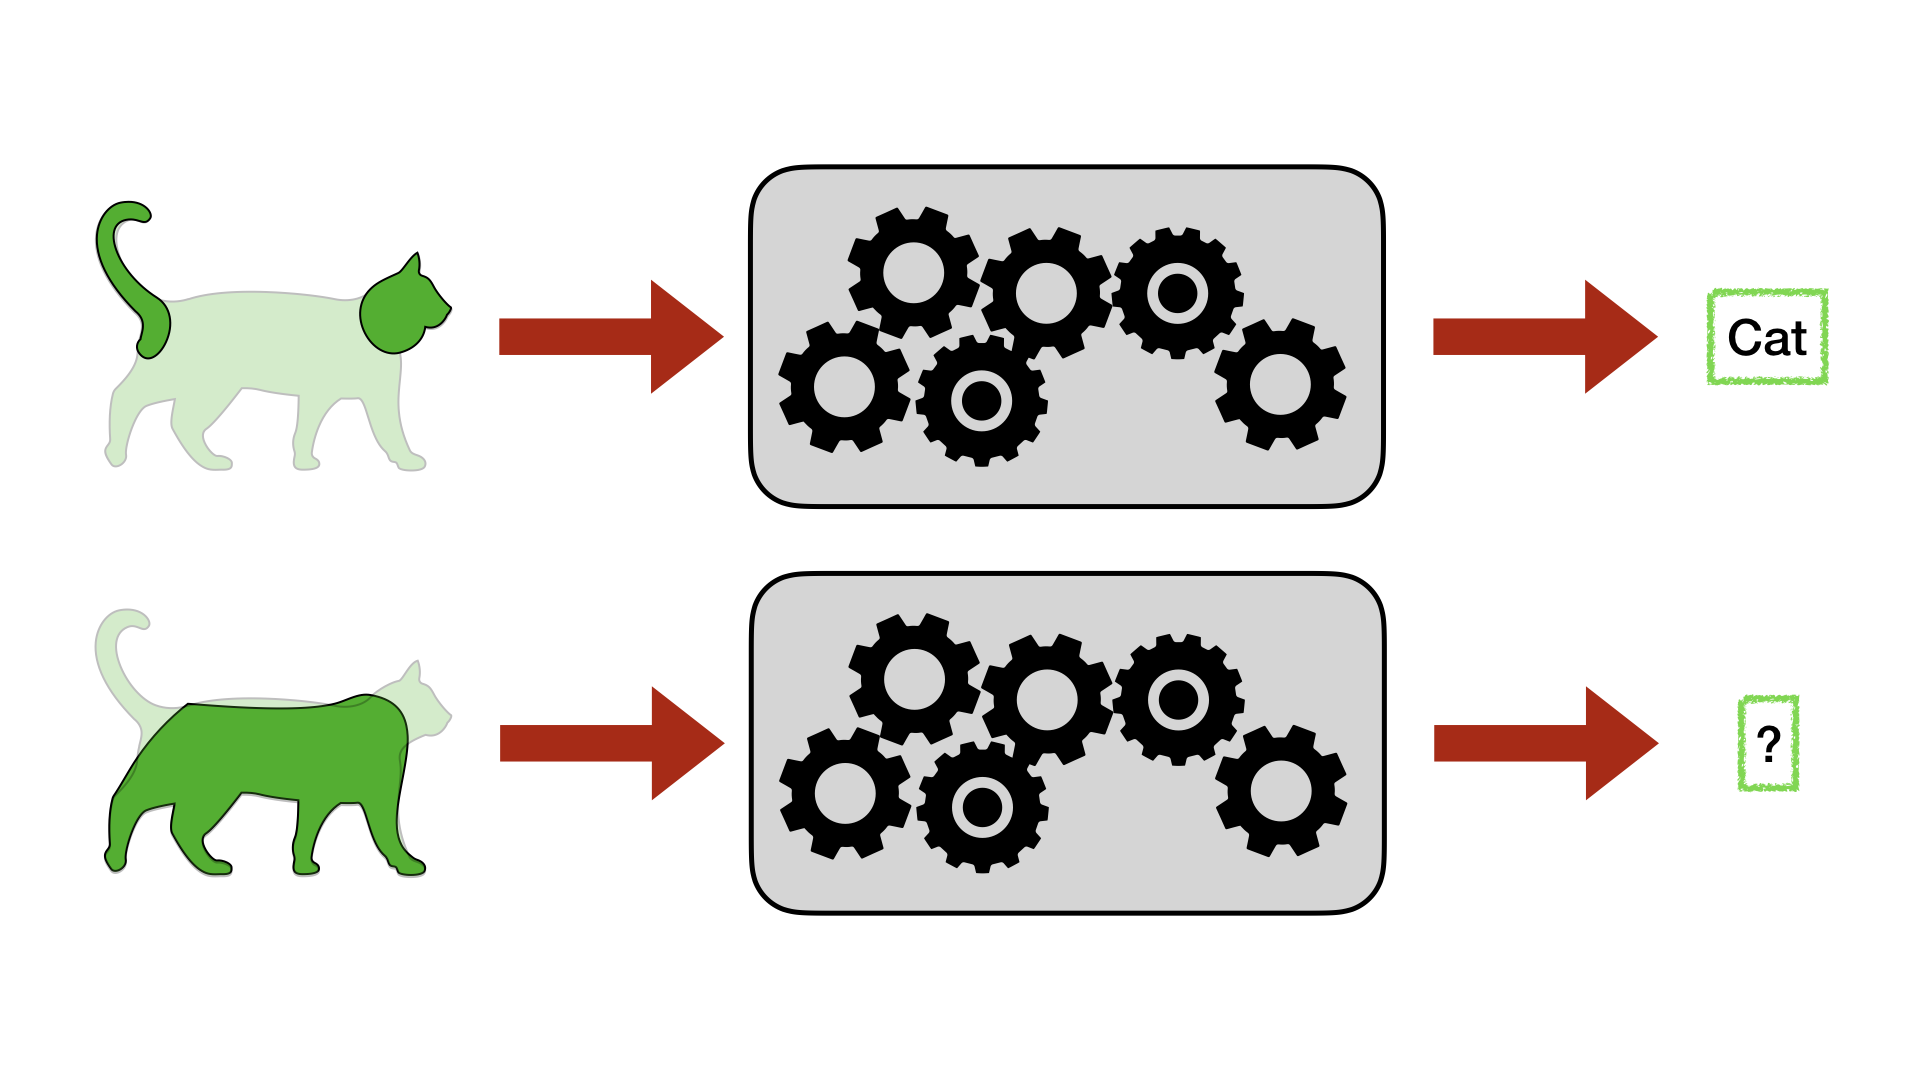
\includegraphics[trim={0 3cm 0 3cm},clip,width=0.9\textwidth]{diss/1_intro/figs/feat_select.png}
    \caption[Visualization of feature selection]{An example of identifying specific features important to the learning task.}
    \label{fig:feat_select}
\end{figure}
\paragraph{Feature Selection.} 
With more complex models $f$ compared to the linear case above, newer ``black-box'' methods have been developed for identifying important features. From the more pure statistics side, scan statistics~\citep{scanstat,scanstatlrt} allow for a structured ``scanning'' over the input space, skipping subsets unlikely to provide additional information for the measure of interest.
Further on the deep learning side, adaptations of sensitivity analysis, via noise addition and perturbations have found success~\citep{yeung2010sensitivity,zhang2015sensitivity}, alongside activation mapping~\citep{cam,selvaraju2017grad}.
These methods typically generate an analagous ``weighting'' over the input space, identifying features most salient for the specific task (Figure~\ref{fig:feat_select}).

\begin{figure}
    \centering
    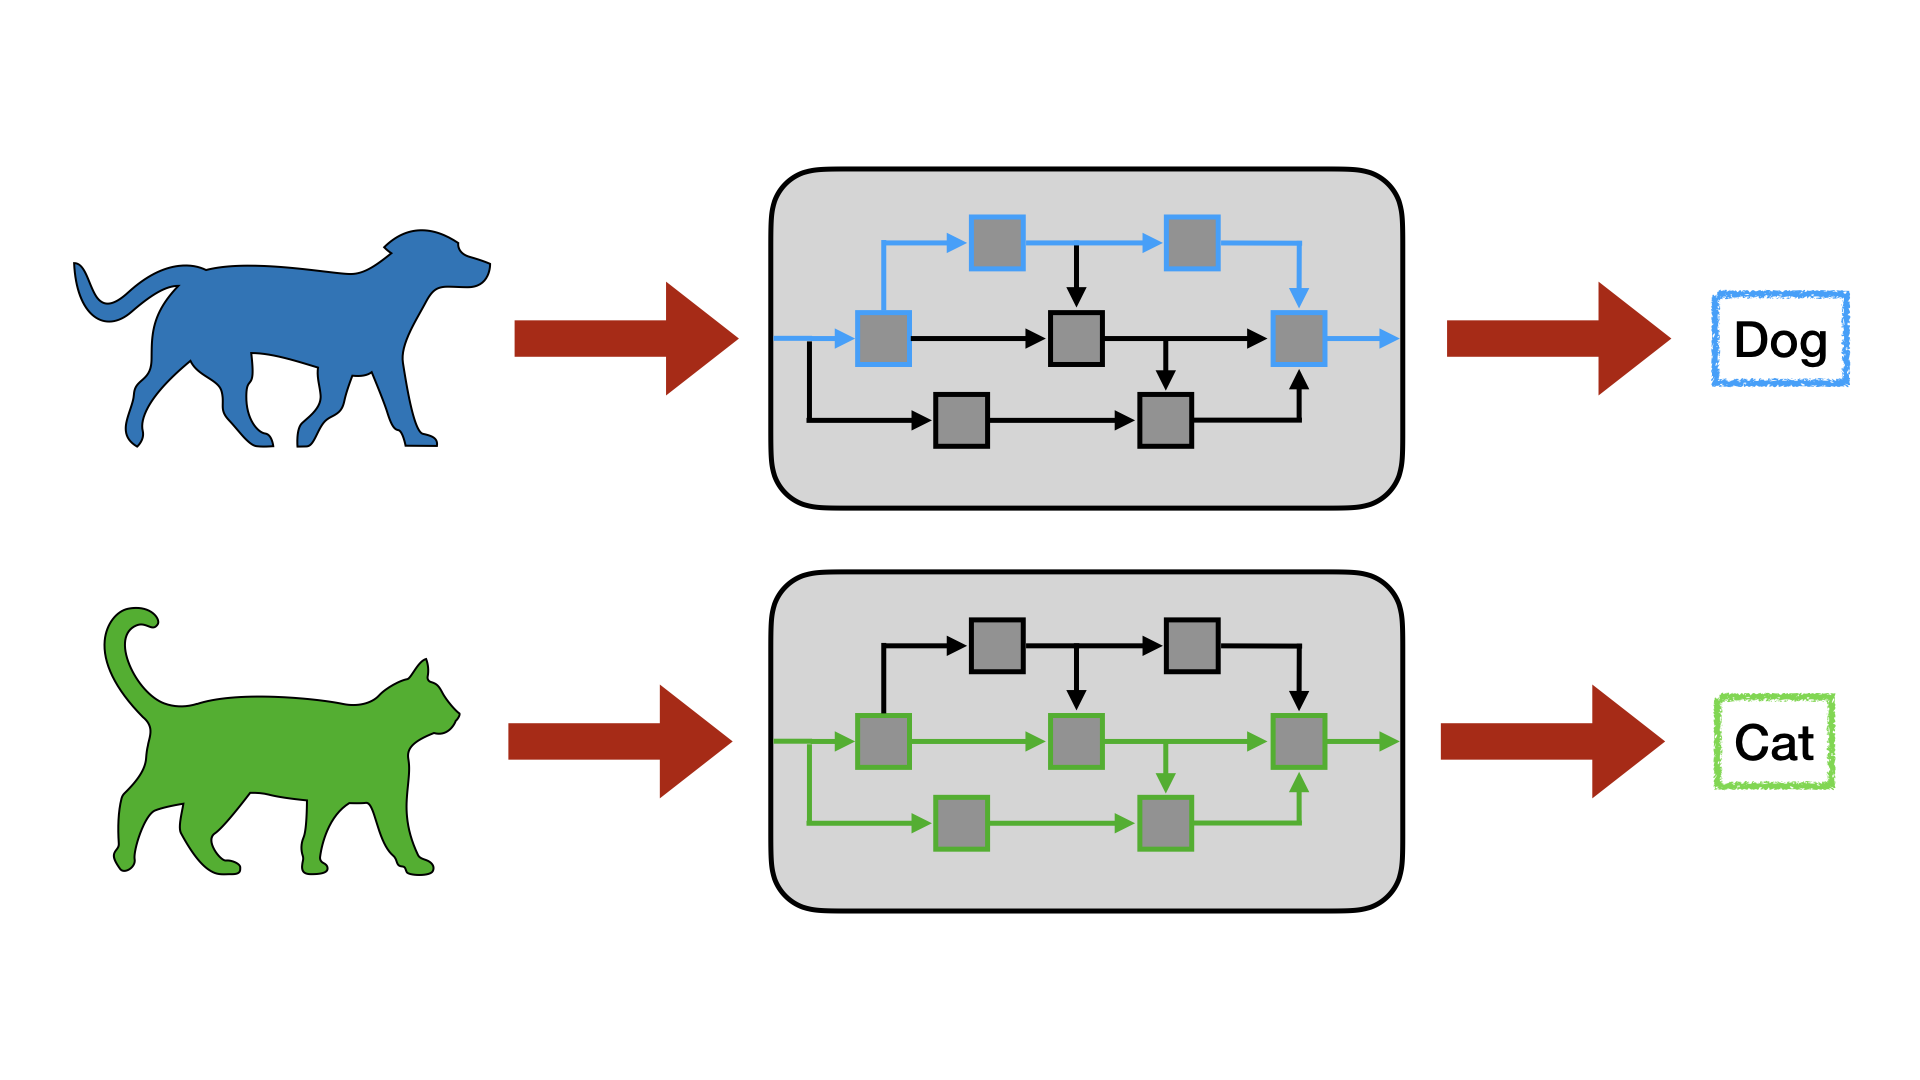
\includegraphics[trim={0 3cm 0 3cm},clip,width=0.9\textwidth]{diss/1_intro/figs/param_select.png}
    \caption[Visualization of parameter selection]{An example of identifying specific parameters important to the learning task.}
    \label{fig:param_select}
\end{figure}
\paragraph{Parameter Selection.} 
Selection in the model space generally takes two forms. First, as a prior, restriction, or assumption over the model space, and second, as a post-hoc method for an ``explainable'' proxy.
Regularization, sparsity, and gating methods are often used independent of the type or size of the model, to encourage the solution to fall within a specific region of the model space.
% In non-deep settings these methods come with strong theoretical guarantees. 
The theoretical underpinnings of these methods in deep learning are still being actively researched~\citep{hardt2016train,jacot2018neural,neyshabur2014search}, but the methods have nonetheless been effective in practice. 
On the post-hoc side, of particular interest are the parameters relevant to specific regions of the input space \textit{after} training (Figure~\ref{fig:param_select}). Here, recent analysis of deployed networks has shown this to be true~\citep{bau2017network,fong2018net2vec}, and current work continues to explore these network regions to aid in interpretability and explainability.

\paragraph{Sample Selection.} Many methods have been developed for outlier detection within training or testing sets~\citep{huang2020feature,ren2019likelihood} \textit{after} training, as well as methods for understanding sample influence~\citep{koh2017understanding,golatkar2020eternal,huang2020feature} . ``In-the-loop'' methods for accounting for ``outlierness'' behave similarly to accounting for group or individual fairness while training~\cite{mehrabi2021survey}. Unfortunately, once samples are identified in some manner, post-hoc adjustments to a trained model are generally very difficult. Recent work has focused on ``unlearning'', or removing a sample's influence on a model without retraining. If specific samples can be uniquely identified, performance and privacy reasons may require these specific interventions to reduce the ``influence'' of that sample subset.
\begin{figure}
    \centering
    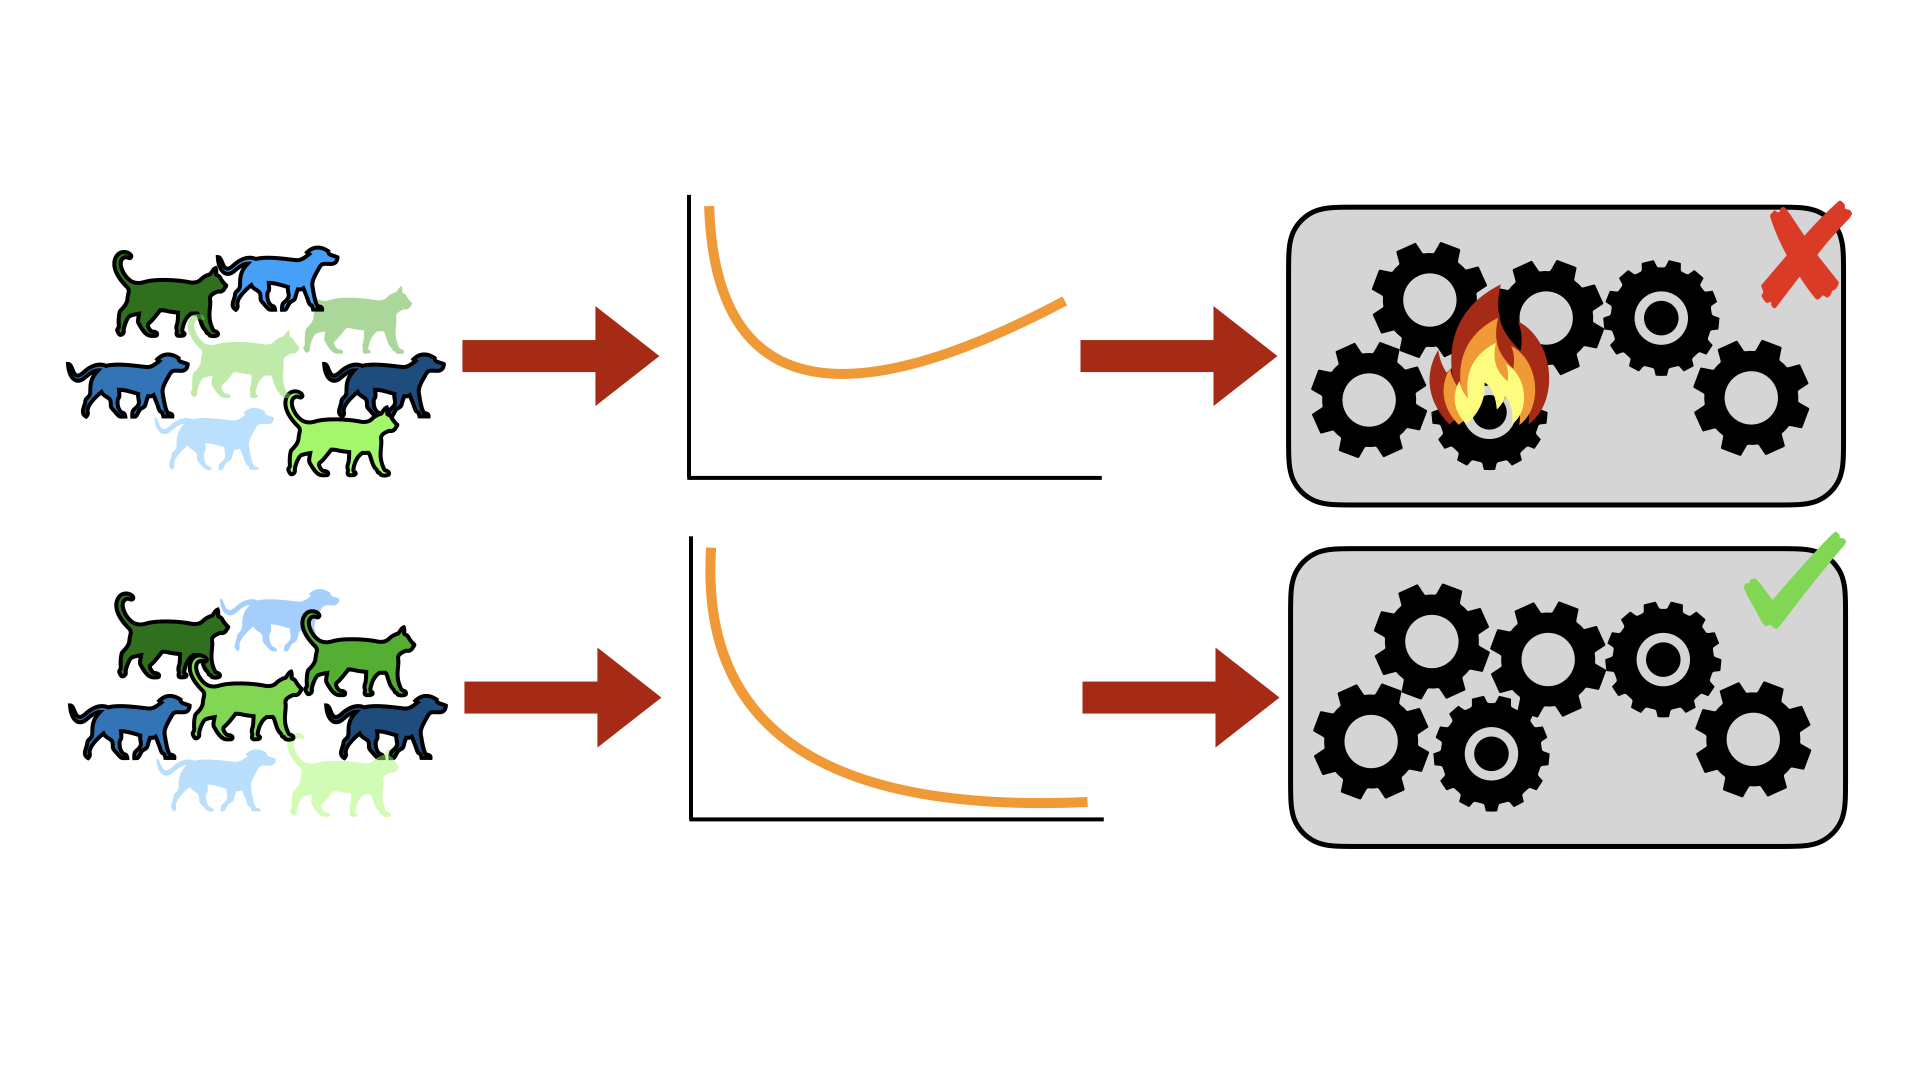
\includegraphics[trim={0 4.5cm 0 4cm},clip,width=0.9\textwidth]{diss/1_intro/figs/sample_select.png}
    \caption[Visualization of sample selection]{An example of identifying specific samples important to the learning task.}
    \label{fig:sample_select}
\end{figure}


\begin{mdframed}[style=MyFrame]
\textbf{ Thesis Goal: }
\em Identify, construct, and evaluate methods for \textbf{efficient} subset identification in modern machine learning feature, model, and input spaces.
\end{mdframed}

\section{A Few Motivating Examples}
Consider a traditional machine learning classification task in which we would like to predict whether an individual has a specific disease condition based on a medical resonance image (MRI) scan of their brain. Our input feature $x$ may consist of a 3D-array of values in $\RR^{\cI\times \cJ\times \cK}$ measuring some intensity of the imaging modality at each voxel, indexed by a tuple $(i,j,k) \in (\cI,\cJ,\cK)$.
Our outcome variable $y$ may simply be a binary label of whether the input scan has been labeled by a radiologist as one demonstrating typical disease characteristics.
Using an off the shelf 3D convolutional neural network with adjustments to match our input size, we can very quickly set up and train a system to predict disease presence with a high degree of accuracy.

\paragraph{Example 1.}
With a prediction for a specific scan, or predictions over a number of scans, we might be interested in identifying which regions of the brain are most important for diagnosis. These regions, $R \subset \cR:=\RR^{x\times y\times z}$, can be specific groups of pixels in the image that may correspond to known functional networks. Methods such as attention and class activation maps may work here, but there are a few issues. The number of samples available to learn a model is very small compared to the both the dimension of the input and the number of parameters in the model, i.e., $n \ll p$ and $n \ll d$. Thus it is very easy to overfit, and for areas of interest to be associated with intricacies of particular input data rather than true, real differences defined by the disease.

Furthermore, recent medical imaging studies have moved past simple difference detection: trends over time, and the ability to predict {\em future} disease development have by far become the setting of most interest.
Given an image of a healthy individual, is it possible to predict what their scan, or their future disease diagnosis, may be up to 10, 20, or more years in the future?
If a number of scans have been collected over some timeframe, can the \textit{trajectory} of the individuals' development be extrapolated to estimate progression?
As traditional models extended for temporal analysis grow in both size and complexity,
a number of subproblems explicitly related to model and input subspaces arise. In this thesis we address two such problems: \textbf{statistically rigorous identification of temporally evolving subsets}, and \textbf{characterizations of deep models that enable efficient training of recurrent models with large scale time-varying data}.
    
\paragraph{Example 2.}
With the rapid growth of AI and machine learning applications has come valid concerns regarding both guarantees of privacy.
Recent technology legislation has made the importance clear in all aspects of data use,
and particular projects and groups have demonstrated that machine learning is not independent of
this need \citep{Exposing}.
A new issue raised within this intersection is the ``right to be forgotten".
If a model has been trained with a particular users' data, 
they should have some recourse or right
to both remove their data from the training set,
and also know that the model has not learned from their data.
On the surface, this poses a significant problem for model builders
and organizations that spend large amounts
of time and resources in 
training deep learning models.

In the medical imaging example above this is especially important: with fewer samples it is more likely that information about any particular one could ``leak'', and the model's performance may degrade significantly as a relatively large percentage of it's training data is removed.
Thus tailored methods must be developed to ensure both privacy and performance, without requiring full retraining.
As we will see, 
\textbf{identification of model parameter subsets}
that are particularly important
for a particular sample's influence
in a model enables \textit{efficient machine unlearning}.

\paragraph{Example 3.}
From an alternative perspective, we may want to identify specific samples rather than have them specified a priori.
Traditionally a rigorous area of study under classical statistics, outlier detection and accounting have become a subfocus for many within the machine learning community as well \citep{golatkar2020eternal,golatkar2020forgetting,huang2020feature,ren2019likelihood}.
While subgroups of input samples may be outliers, it is more often the case that they represent known heterogeneity within the data. 
These differences may be marked using 
group information known a priori, and 
most learning tasks aim to learn tasks
in a \textit{subgroup-independent} manner.
In our disease prediction model above,
these groups could simply be stratified by the type of scanner used to acquire the image, but it could also
be a systematic difference correlated with some protected attribute. {\color{red} sentence about original brain atlas for registration being eurocentric}
This can directly lead to disparate performance and results on \textit{all} individuals outside of that group.
Optimization and regularization methods with this focus come under the umbrella of model fairness.
However, many existing methods do not scale well to larger models or as the number of subgroups grows, as is often the case when intersections of protected classes must be considered. Here we identify and construct a particular solution for \textbf{groupwise fairness that enables efficient in the loop fairness regularization}.

% What features are most important for prediction?
% Which samples were most important for my training?
% Can we understand when a model is certain or uncertain about its output?
% Are there layers in my network that have learned a particular subtask?
% Questions of robustness, bias, influence, fairness, and importance have become central questions to contemporary machine learning research \citep{doshi2017towards,mehrabi2021survey,amodei2016concrete}.
% machine learning, etc.

% Feature selection in the case of
% typical regression or classification 
% takes some form of learning parameters $\theta$ that allow for $\hat{y} = f_\theta(x)$ to be close to the true outcome of interest $y$.
% While forms of data $X := (x,y)$ may simply be continuous and real-valued, modern machine learning has greatly expanded formulations of the classical learning problem to include a wide variety of structured learning problems~\citep{nowozin2011structured}. 
% Consider the case when a high-dimensional input is used to predict an output with a highly-parametrized model. 
% Once learned, obvious questions arise as discussed above: are there specific low-dimensional spaces in either the input or the model space that are most important or necessary for the global learning problem of interest? Are there specific subspaces associated with particular subproblems of the global problem?
% The machine learning literature has come up with a number of ways to identify analogs of these spaces, 
% including extensions of sensitivity analysis to deep learning~\citep{yeung2010sensitivity,zhang2015sensitivity}, and constructing and identifying nonzero model subsets via particular model choices such as activations~\citep{selvaraju2017grad} and regularizers.
% In classical settings these are well understood: decision trees naturally provide ease of interpretibility via the information used to choose splits, and both linear and kernel support vector machines have been analyzed to provide for measures of sample importance via distances to the margin as well as feature importance via weights defining the learned hyperplane~\citep{Mitchell97}.
% Attention and saliency maps have emerged as popular new methods,
% given their ease of implementation and interpretation~\citep{sutskever2014sequence,vaswani2017attention,selvaraju2017grad}.
% By learning dimensions of a given input that are particularly important, either in a hard (binary) or soft (continuous weighting) manner, model builders are better able to understand and interpret what a model has learnt.
% The specific ideas of attention notwithstanding, many of these existing methods are far removed from traditional hypothesis testing frameworks.
% While some work has begun in this direction~\citep{tansey2018black},
% there remains a gap in direct identification of subsets and structures in these spaces that can be defined in statistically rigorous manners.

% \begin{figure}
%     \centering
%     \includegraphics[width=0.5\textwidth]{example-image-a}
%     \caption[A simple subset selection example]{\color{red} Identifying and selecting in MRIs, subset, sample, model ID.}
% \end{figure}

% \paragraph{A specific example.} 

% ------------------------------------------

% below here will be moved and arranged with the "selection" sections and here if relevant

% ------------------------------------------

% While attention can be directly applied to the network in order to identify ``hotspots" in the input space relating to the learned classification task, 
% given the high-dimensional nature of the input
% and the relatively small sample size 
% associated with medical imaging data, 
% it is very likely that an area of interest identified
% may be an intricacy of the training samples used rather than truly a region of disease signal.
% Class activation maps (CAMs) may be unclear, and can often associate with image artifacts unrelated to the scientific task~\citep{adebayo2018sanity}.
% Methods of generalization may help to increase confidence in identified regions, but statistical guarantees often remain out of reach.

% Furthermore, most recent problems associated with medical data have moved past simple difference detection: trends over time, and the ability to predict {\em future} disease development has by far become the setting of most interest.
% Given an image of a healthy individual, is it possible to predict what their scan, or their future disease diagnosis, may be up to 10, 20, or more years in the future?
% If a number of scans have been collected over some timeframe, can the \textit{trajectory} of the individuals' development be extrapolated to estimate progression?
% As traditional models extended for temporal analysis grow in both size and complexity,
% a number of subproblems explicitly related to model and input subspaces arise. Here we address two such problems: \textbf{statistically rigorous identification of temporally evolving subsets}, and \textbf{characterizations of deep models that enable efficient training of recurrent models with large scale time-varying data}.

% A sample's particular influence on model parameters aside, the identification of influential samples or subsets of samples more generally is of independent interest. 
% Traditionally a rigorous area of study under classical statistics, outlier detection and accounting have become a subfocus for many within the machine learning community as well \citep{golatkar2020eternal,golatkar2020forgetting,huang2020feature,ren2019likelihood}.
% While subgroups of input samples may be outliers, it is more often the case that they represent known heterogeneity within the data. 
% These differences are typically marked using 
% group information known a priori, and 
% most learning tasks aim to learn tasks
% in a \textit{subgroup-independent} manner.
% Optimization and regularization methods with this focus come under the umbrella of model fairness, and instead of identifying and boosting independences within the model or data, we aim to minimize them.
% However, many existing methods do not scale well as the number of subgroups grows, as is often the case when intersections of protected classes must be considered. In the sequel we identify and construct a particular solution for \textbf{groupwise fairness that enables efficient in the loop fairness regularization}.

\begin{mdframed}[style=MyFrame]
\em 
Here we focus our effort on identifying these important subsets of model, feature, and sample space for feature association, model size reduction, model unlearning, and, fairness. Specifically, taking advantage of both existing statistical and geometric methods, we develop new methods for localizing subsets in a range of settings from hypothesis testing to deep learning.
\end{mdframed}

\section{Thesis Scope and Contributions}

We explore the intersections of classical statistical and geometric constructions with modern machine learning methods. 
Figure~\ref{fig:scope} shows the overall scope projected along three axes: feature, parameter, and sample spaces.
Below we briefly introduce the main problems studied in this thesis.
\begin{figure}[!ht]
    \centering
    % \includegraphics[width=0.99\linewidth]{scope.pdf}
    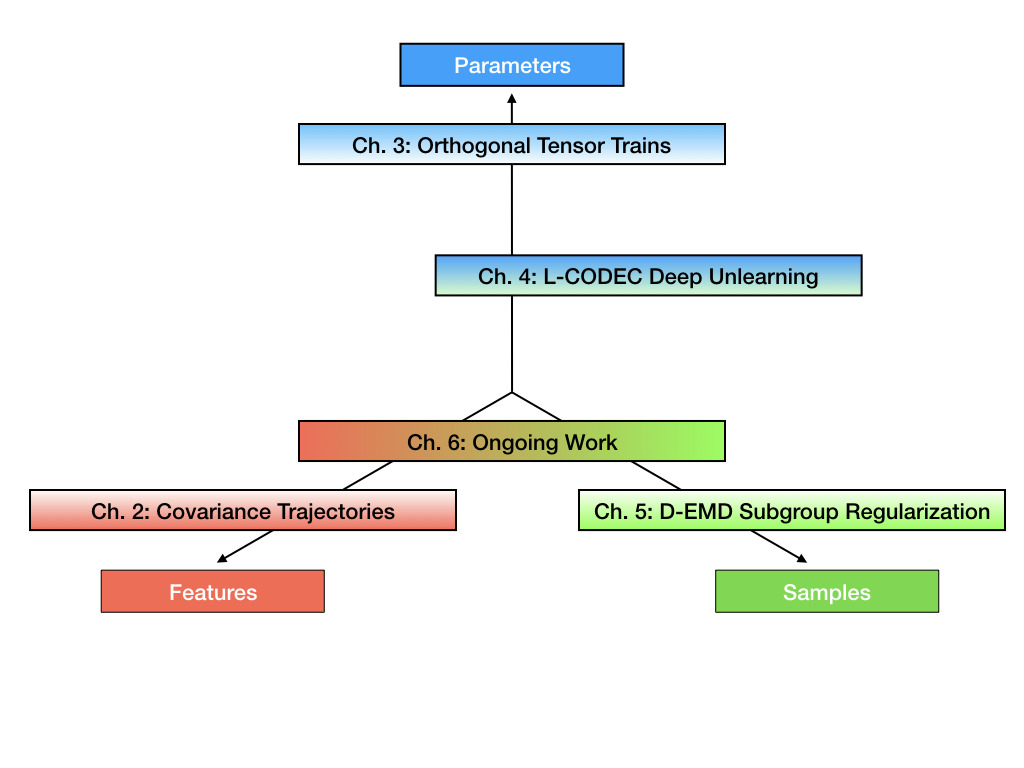
\includegraphics[width=0.95\linewidth]{diss/1_intro/figs/thesis_scope.png}
    \caption[Thesis Scope]{Thesis scope, projected over three representative axes. {\color{red} update chapter numbers shift by 1}}
    \label{fig:scope}
\end{figure}

\subsection{Second-Order Modeling and Group Difference Analysis over Time}

Recent results in coupled or temporal graphical models offer schemes for estimating the relationship structure 
between features when the data come from
related (but distinct) longitudinal sources. A novel application of these ideas is for analyzing group-level differences, i.e., in identifying if {\em trends} of estimated objects (e.g., 
covariance or precision matrices) are different across disparate conditions (e.g., gender or disease). Often, poor effect sizes make detecting the \textit{differential} signal 
over the {\em full} set of features difficult: for example, 
dependencies between only a {\em subset of features} may manifest differently across groups.
We first suggest
a parametric model 
for estimating trends in the space of $\SPD$ matrices as a function of one or more covariates.
We will then generalize scan statistics to graph structures, 
to search over distinct subsets of features (graph partitions) whose temporal dependency structure may show statistically 
significant group-wise differences.
We will theoretically analyze the Family Wise Error Rate (FWER) and bounds on Type 1 and Type 2 error. 
On a cohort of individuals with risk factors for Alzheimer's disease (but otherwise cognitively healthy), 
we 
find scientifically interesting 
group differences where the default analysis, 
i.e., models estimated on the full set of features, do not survive reasonable 
significance thresholds. 
% Preliminary work on this was published in \citep{covtraj}.


\subsection{Efficient Tensor Representations for Feasible Temporal Deep Learning}

Modern deep networks have proven to be very effective for analyzing real world images.
However, their application in medical imaging is still in its early stages,
primarily due to the large dimension of three-dimensional images, requiring enormous convolutional or fully connected layers --
if we treat an image (and not image patches) as a sample. 
These issues only compound when the focus moves towards longitudinal analysis
through recurrent structures, and when a point estimate of model parameters is insufficient 
in scientific applications where a reliability measure is necessary.
Using insights from differential geometry, 
we will adapt 
the tensor train decomposition to construct networks
with significantly fewer parameters,
allowing us to train powerful recurrent networks on whole brain image volumes. 
We analyze 
the \textit{orthogonal tensor train},
and demonstrate its ability to express a standard network layer both theoretically and empirically.
We 
demonstrate its ability to 
effectively reconstruct whole brain volumes
with faster convergence and stronger confidence intervals
compared to the standard tensor train decomposition. 
We provide code and show experiments on the ADNI dataset
using image sequences to regress on a cognition related outcome.
% Preliminary work on this was published in \citep{ott}.

\subsection{Practical Unlearning via Large-Scale Conditional Independence Testing}

%With AI systems extensively using personal %data for model training, 
Recent legislation has
led to interest in {\em machine unlearning}, i.e., removing specific training samples from a {\em predictive} model as if they never existed in the training dataset. 
Unlearning may also be required due to  corrupted/adversarial data or simply a user's updated privacy requirement.
For models which require no training ($k$-NN), 
simply deleting the closest original sample can be effective. 
%However, it is not clear how such approaches can be used to unlearn 
%models that contain rich information learned from the original data.
But this idea is inapplicable to models which learn richer 
representations.
%from data. 
%Recently, optimization-based unlearning estimators have been proposed, but 5their 
Recent ideas leveraging optimization-based updates
scale poorly with the model dimension $d$,  
due to 
inverting the Hessian of the loss function. %with an overall cost of $O(d^3)$ 
%is prohibitive.
We describe
a variant of a new conditional independence coefficient, 
L-CODEC, to identify a subset of the model parameters with the most semantic overlap on an individual sample level. 
Our approach completely avoids the need to invert a (possibly) huge matrix. 
By utilizing a Markov blanket selection, 
we find
that L-CODEC is also suitable for deep unlearning,
as well as other applications in vision.
Compared to alternatives, L-CODEC makes approximate unlearning possible 
in settings that would otherwise be infeasible, 
including vision models used for face recognition, 
person re-identification 
and NLP models that may require unlearning samples identified for exclusion.
% Preliminary work on this will appear in \citep{lcodec}.


\subsection{Reducing Subgroup Fairness via High Dimensional Earth Mover's Distances}

Optimal transport has recently emerged as a useful tool for machine learning through its connections with geometry, statistical machine learning, and through practical algorithms. Existing methods that leverage optimal transport often  regularize using  a Wasserstein metric or by computing barycenters, for example. %which are effective when distributions are continuous and known, or when measures of interest are discrete.
% Our formulation allows for a discretization of continuous measures that drop in directly to classical  formulations of the Earth Mover's Distance. 
We leverage optimal transport, except that we take advantage of a recently-introduced algorithm that computes a generalized earth mover's distance.
Not only is this algorithm computationally cheaper to compute compared to existing barycentric measures, but our method has the additional  advantage that gradients used for backpropagation can be directly read off of the forward pass computation, which leads to substantially faster model training.
We provide technical details about this new regularization term and its properties, 
and 
experimental demonstrations of improved training speed over existing Wasserstein-style methods.

{\color{red}
\subsection{Understanding Latent Spaces via Conditional Independences}

The final chapter of this thesis applies some of the tools developed above in the analysis of latent spaces in recent large scale models.
% In these studies, 
% we aim to identify conditionally independent features and subjects that are particularly important to the prediction and estimation of
% key disease outcomes,
% as a function of a number 
% of demographic, neuropsychological,
% genetic,
% and imaging data collected as 
% part of an ongoing consortium 
% to understand the progression
% of Alzheimer's disease in younger, 
% asymptomatic populations.
% In what follows we present
% exploratory analysis
% on a small, easily 
% digestible subset of the available data,
% that lays the foundation for
% further analysis.
}
% This work is the most forward looking, and aims to be a stepping stone toward a rigorous 

\section{Outline}
Chapter 2 covers the essential background necessary for the developments presented in the following chapters, including specifics of graphs and hypothesis testing, as well as relevant modern methods for learning and optimization.
In Chapters 3 through 7, we describe four perspectives to address subset identification.
Chapter 3 explores and focuses on the identification of feature subsets varying over time.
In Chapter 4 we describe a method of constraining the parameter space in a particular manner
that enables more efficient large scale neural networks.
Next, Chapter 5 provides a solution to the machine unlearning problem,
enabled through a particular conditional independence parameter selection scheme, vastly reducing network update costs.
Chapter 6 ends with a unique solution to subgroup fairness, 
where we take advantage of an efficient solution to
the $d$-dimensional earth mover's problem
to regularize large models when the number of subgroups can be large.
{\color{red} Chapter 7 describes future work, focused on applying a particular solution from Chapter 5 to understanding relationships among features in latent spaces learned by large generative models.}


%%%%%%%%%%%%% 
% Some old stuff

% Significant progress in the modern development of machine learning has
% been built upon connections and patterns identified across myriad
% interdisciplinary fields of study.
% Up through the mid 2000's, 
% many of these methods were inspired by and interested in 
% highly focused and constrained problems. 
% With a reasonably sized input domain, could a model of roughly equal size be used to
% predict some output?
% Linear regressors, decision trees, and support vector machines were all answers to these questions, with their own
% varying degrees of scaling and complexity.
% These methods necessitated carefully constructed formulations with specific restrictions to the learnable function class,
% enabling straightforward analysis 
% for provable performance guarantees 
% and easy identification of critical training samples and important input features.

% Contemporary machine learning, however, has a vastly different modus operandi. 
% Driven in large part by the exponential growth of available computation via Moore's Law, \textit{deep learning} has fallen squarely in the realm of \textbf{over-parameterized} models.
% With these overparametrizations and computation capacity, the typical learning questions posed as maximizing accuracy or reducing error have largely been addressed for even large scale problems.
% As such, complementary questions have led to subfields focusing on other performance measures, such as robustness, fairness, interpretability, and explainability.
% Many solutions to these questions end up looking back at answers found for the under- or non-parametrized settings.
% While nascent, these approaches 
% attempt to fill the gap between
% statistical and deep models to enable similar measures of sample influence, feature importance, and model analysis. 
% Most notable amongst these newer approaches is that of (Self)-Attention in Neural Networks \citep{sutskever2014sequence,vaswani2017attention}.
% Other proposals 
% end up looking back at the types of analysis typical of those more classical under-parametrized or nonparametrized methods.

% Not limited to previous developments in learning or computation theory, the arguably most valuable contributions toward the exponential reduction in model error can be attributed to influences and intuitions taken
% from biology, psychology, neuroscience, and even XXX \citep{srivastava, etc}.
% Perhaps one explanation as to why this phenomenon exists may be attributed to the way in which deep learning evolved. 
% The classical learning goal of function approximation lends itself nicely to a system which allows for arbitrary complexity via simple changes (e.g., addition of neural network layers). % Foundational works building on the original neural networks particularly have taken advantage of constraining this space of functions to search over: 
% the most seminal case being those of convolutional filters for imaging data. 
% While ``constraints" of this form have helped tremendously in model performance on modern vision and language machine learning tasks (GANs, Recurrent Networks, Residual Layers, Transformers, etc.), the ability to identify \textit{subsets} of important samples, input features, and model parameters has lagged significantly behind the development of these methods.
% Recently larger interest has been taken by the community to understand and interpret models with this view, only after extremely large and opaque models have become ubiquitous.
%This lag directly explains the more recent interest in developing methods for understanding and interpreting large scale machine learning models. % DEMD
% \chapter{Introduction} \label{chap:intro} 

Modern applications of machine learning in a broad range of industrial and consumer-facing systems have become ubiquitous.
Most interactions with daily technologies now intrinsically involve 
a request to some ``smart`` system in the ``cloud'', 
where those interactions range from
a request for map directions 
to simply loading a webpage.
Neural network models, and the recent advances of deep learning,
have enabled these systems that 
make such applications possible.
These models have achieved
human-level performance on learning tasks
including image classification~\citep{resnet,alexnet}, image segmentation~\citep{segmentation}, video analysis~\citep{zhang2016video}, text understanding and generation~\citep{bert,gpt}, and have slowly begun to solve more fundamental scientific problems such as protein folding~\citep{protein} drug discovery~\citep{drugdisc}, and medical diagnosis~\citep{diag}.
While this performance is largely attributed to model size,
the abundance of high quality training data
has equally contributed to real world performance,
enabling model training over millions of real world samples~\citep{imagenet,laion},
and potentially billions of synthetic samples via environment simulation~\citep{mcts}.

While deployment in some domains (recommender systems, object detection) may benefit almost unconditionally from this vastly expanded capability, rightful hesitancy has limited their widespread use in particular applications where impacts on individuals, people, or environments may be at stake.
These ``last mile'' concerns take a few forms.
% Because a completely accurate model is still out of reach, an important question that needs to be answered is: which inputs or individuals are being given incorrect outcomes, and why?
% maybe a sentence suggesting unlearning/removal
In mission critical applications such as medical diagnosis, 
the impact of an error can be extremely large,
even if a misprediction happens extremely infrequently.
Additionally, large scale model training and architecture search
can require exorbitant amounts of energy producing high emissions,
and their scale can limit market participants
to only large actors with vast existing resources.
The accessibility and effectiveness of these models can also vary significantly based on the training data, and disparate outcomes can be exacerbated by existing social inequity.

While existing human or ``natural'' systems that these models aim to assist are not perfect, 
our real world has developed norms and regulations that 
enable them to function.
A medical diagnosis might require a physician to explain what symptoms led them to that particular conclusion.
Energy metering and carbon taxes may be applied to limit
emissions.
Regulatory satisfaction may require 
analysis proving equal opportunity,
or that specific protected classes
are not used in decision making.
% Specifically, these can include ideas as simple as the Hippocratic Oath and medical malpractice insurance, to asking your doctor what symptoms lead them to a particular diagnosis.
These ideas are difficult to directly translate to automated machine learning systems,
but proxies have been identified that we can build upon.

These norms and regulations answer a number of questions we may also try to pose to our machine learning models.
What is the cost to learn this task?
What led to this particular outcome?
Why is this outcome different from another?
% We will explore how these questions can be formulated concretely. 

If the answer to these questions is negative or unknown,  follow-up questions all take an interesting form:
Can we learn a smaller model with similar performance? 
Can we identify the most important features? 
Which individuals or groups are being treated unfairly, and can we change that?
These questions ask us to identify a \textit{subset} of some relevant set, dependent on setting, and this identification is our focus here.

% Moving specifically to machine learning methods,
Taking a step back, let's take a look at a representative system. Figure~\ref{fig:dl} illustrates a typical learning pipeline. 
A dataset is collected and used to train a model, by minimizing the error over
those samples in the dataset (top).
A ``sample'' can be a single measured value, or it can
be a large, highly structured object with many ``features.''
The model is made up of some ``parameters'' that are 
tuned during training to learn a good predictor over the training dataset.
This model is then used to predict, or \textit{infer}, on new
data seen ``in the wild'' (bottom).
Our questions above are formally asking to identify \textit{subsets of these objects}: is a subset of the model parameters sufficient for learning? Which subset of the features are important for a prediction? Which subset of the dataset exhibit a specific attribute?
\begin{figure}
    \centering
    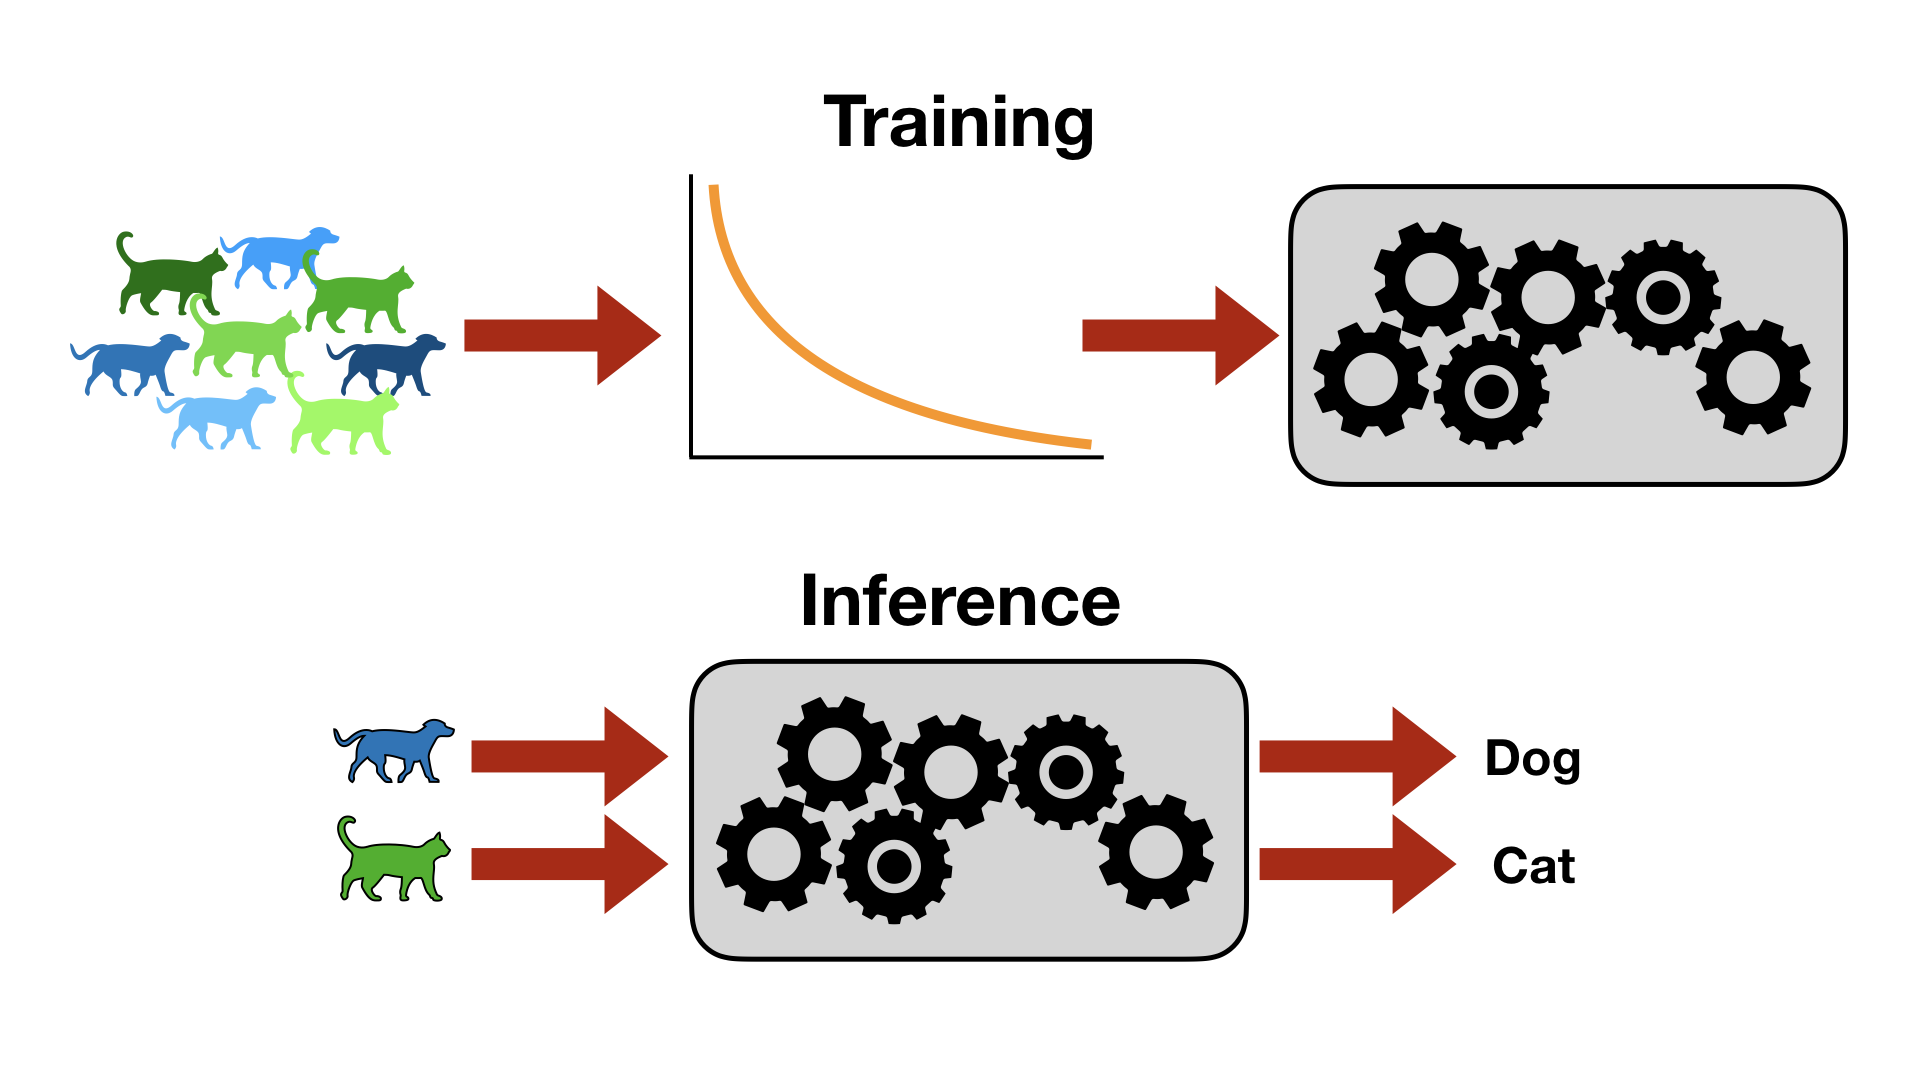
\includegraphics[trim={0 3cm 0 3cm},clip,width=0.95\textwidth]{diss/1_intro/figs/dl.png}
    \caption[Modern machine learning pipelines]{Machine learning training and inference visualization.}
    \label{fig:dl}
\end{figure}

% \textit{Explainability} can be seen as identifying important features of the input, as well as parts of the model (parameters) that ``light up`` for that input. \textit{Fairness} can be evaluated via measures over subsets of the data that correspond to specific groups. 

\begin{mdframed}[style=MyFrame]
\em 
\textbf{This thesis} focuses its main efforts on identifying these important subsets of model, feature, and sample space, to enable answering questions necessary for mainstream adoption of machine learning methods.
\end{mdframed}

% In this dissertation, we explore the sizes of these models, samples, and datasets, and 
% analyze under what situations 
% a smaller \textit{subset} of them may be sufficient or important
% for questions that run parallel to standard performance and accuracy measures.

Let us step a bit deeper into a basic illustrative example. In order to ease understanding, we can first begin with a basic formulation of learning methods, from which the questions above can take specific forms. 
Learning methods typically  try to identify a function mapping (model) that is able to complete a specific task at some high level of profficiency.
% In Figure~\ref{fig:dl}, a model is trained using examples of classification task (top), in order to accurately predict the class of a newly provided input (bottom).
% \begin{figure}
%     \centering
%     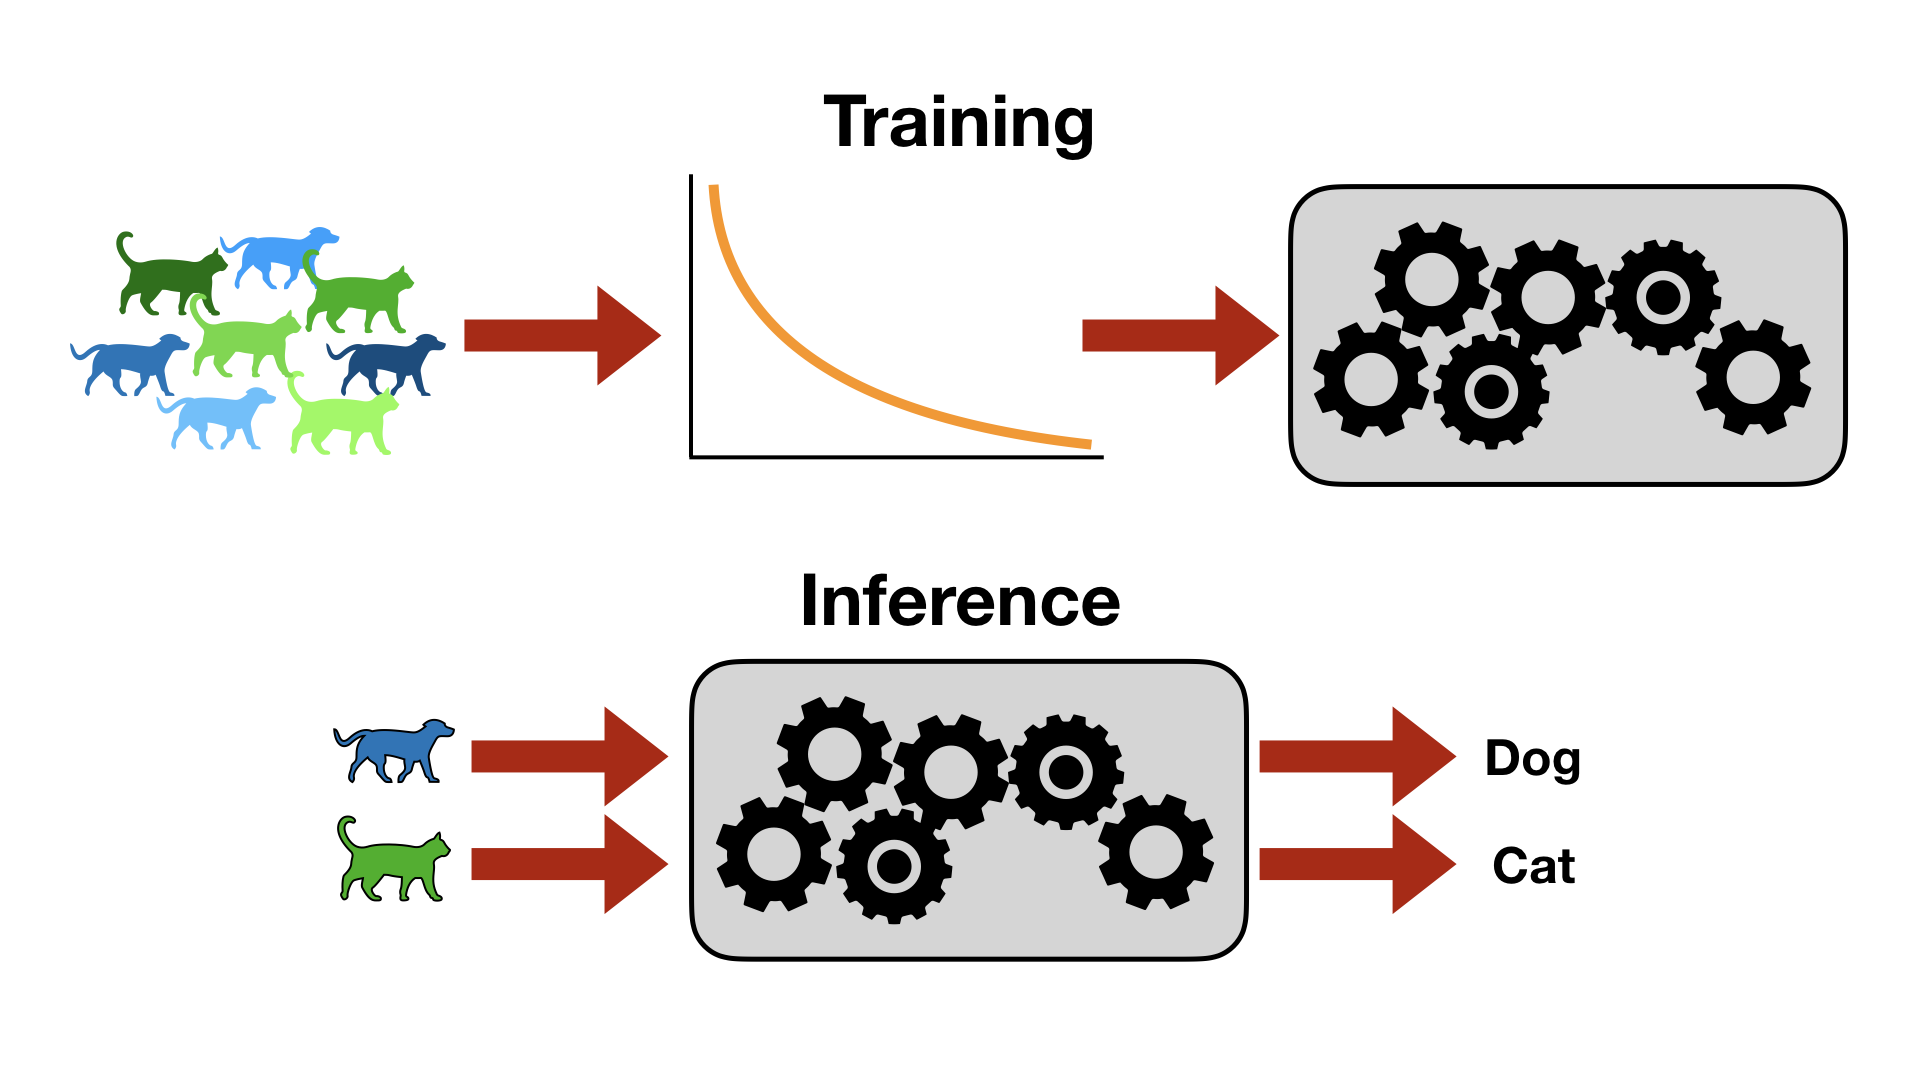
\includegraphics[trim={0 3cm 0 3cm},clip,width=0.95\textwidth]{diss/1_intro/figs/dl.png}
%     \caption[Modern machine learning pipelines]{Machine learning training and inference visualization.}
%     \label{fig:dl}
% \end{figure}
Say we have some dataset comprising of sample pairs $(x,y)$, where we wish to predict $y$ from $x$.
Our prediction, say $\hat{y}$, might be the output of some unknown function $f$ that we attempt to learn from training data. 
Let our approximation to this function be $\hat{y}:=\hat{f}(x)$.
This can take many forms, 
based on assumptions and prior information we may have on the relationships among the data. 
Consider the simple \textit{linear} case,
where we want to learn some parameter $w$ such that $y = w\cdot x$. 
Given $n$ sample pairs $(x_i,y_i)$ indexed by $i$, traditional statistics and optimization literature yield the following \textit{least squares} problem formulation, where we want to minimize the ``squared error'' between the observed values $y_i$ and the predicted $\hat{y}_i:= w\cdot x_i$:
\begin{align}\label{eq:lq}
\hat{f}:=\hat{w} = \mathop{\arg\min}_{w} \sum_{i=1}^n (y_i - w\cdot x_i)^2
\end{align}
This formulation expands without much change to a multi-dimensional form of the input $x$ and respectively, $w$: the canonical case where a number of features, or \textit{covariates} (e.g., symptoms), are used together to predict the outcome (e.g., diagnosis). 
If we are interested in which features of $x$ are important, we can look at the relative values of the learned ``weights'' $w$. In this simple setting, the importance of a feature (say $x^j$) can be exactly determined by the importance of the parameter ($w^j$).
A weight value far from zero may indicate that corresponding feature is important for diagnosis.
% If instead we are interested in which samples are most important, we can use existing methods for sample reweighting or methods that use standard assumptions to efficiently identify important subsets.

In this case and others, traditional statistical learning methods 
have been studied 
for many decades.
Linear regressors, decision trees, and support vector machines
have all been analyzed under these lenses.
% ,
% and as the modern machine learning community
% has returned to these questions recently,
% so has a renewed interest in their methods of analysis.
New research focuses
particularly on the differences
associated with moving from classical \textit{under-parametrized} models to
modern (deep) \textbf{over-parameterized} models: where
the model size vastly outnumbers the number
of input samples.
% , and may even be comparable to 
% the \textit{entire sample space.}
Methods for estimating the number of samples needed,
the time to learn a particular task,
and the generalization ability 
all require new perspectives in this regime.
While nascent, this research
attempts to fill the gap between
statistical and deep models to enable similar measures of sample influence, feature importance, and model understanding. 

\paragraph{A full picture.}
Let us expand our notation from the example above to consider this more general framing.
Consider a dataset $X:=\{x_i\}_{i=1}^n$ of size $n$ where each data point $x_i$ in the set $X$ is drawn from some underlying distribution over the domain $x_i \sim \cX^d$, 
with domain dimensionality (number of features) $d$.
A model $f$ is fit using a parametrization $\theta \in \Theta$,
with $\Theta$ the space of possible parametrizations (models) with some intrinsic dimension $p$. 
%While all three of these problems are closely related, they require different approaches. 
Generalizing the least squares``error measure'' from Eq.~\eqref{eq:lq} to an arbitrary \textit{loss} $\ell$, we have
\begin{align}\label{eq:learning}
    \hat{f}:=\hat{\theta} = \mathop{\arg\min}_{\theta\in\Theta} \sum_{x \in X} \ell(f_\theta(x_i))
\end{align}
From an analysis perspective, 
we might be interested in any one of 
(a) subsets of input features $\cC \subseteq \cX$ that are important for the downstream task,
(b) associating model subsets $\cP \subseteq \Theta$ with specific inputs or groups of inputs, or 
(c) subsets or subgroups of samples $S \subseteq \{X\}$ that are sufficient or representative of the entire dataset.

Crucially, an uninformed search for a subset is computationally infeasible. For a superset of size $n=|X|$, The set of all subsets is the power set, with a size of $2^{n}$! If an identification procedure requires looking over all of these and choosing a ``best'' one by some metric, the procedure will be limited to very small supersets.
Efficient methods have been developed in each of the three contexts above to avoid this exponential search.

\begin{figure}
    \centering
    \includegraphics[trim={0 3cm 0 3cm},clip,width=0.9\textwidth]{diss/1_intro/figs/feat_select.png}
    \caption[Visualization of feature selection]{An example of identifying specific features important to the learning task.}
    \label{fig:feat_select}
\end{figure}
\paragraph{Feature Selection.} 
With more complex models $f$ compared to the linear case above, newer ``black-box'' methods have been developed for identifying important features. From the more pure statistics side, scan statistics~\citep{scanstat,scanstatlrt} allow for a structured ``scanning'' over the input space, skipping subsets unlikely to provide additional information for the measure of interest.
Further on the deep learning side, adaptations of sensitivity analysis, via noise addition and perturbations have found success~\citep{yeung2010sensitivity,zhang2015sensitivity}, alongside activation mapping~\citep{cam,selvaraju2017grad}.
These methods typically generate an analagous ``weighting'' over the input space, identifying features most salient for the specific task (Figure~\ref{fig:feat_select}).

\begin{figure}
    \centering
    \includegraphics[trim={0 3cm 0 3cm},clip,width=0.9\textwidth]{diss/1_intro/figs/param_select.png}
    \caption[Visualization of parameter selection]{An example of identifying specific parameters important to the learning task.}
    \label{fig:param_select}
\end{figure}
\paragraph{Parameter Selection.} 
Selection in the model space generally takes two forms. First, as a prior, restriction, or assumption over the model space, and second, as a post-hoc method for an ``explainable'' proxy.
Regularization, sparsity, and gating methods are often used independent of the type or size of the model, to encourage the solution to fall within a specific region of the model space.
% In non-deep settings these methods come with strong theoretical guarantees. 
The theoretical underpinnings of these methods in deep learning are still being actively researched~\citep{hardt2016train,jacot2018neural,neyshabur2014search}, but the methods have nonetheless been effective in practice. 
On the post-hoc side, of particular interest are the parameters relevant to specific regions of the input space \textit{after} training (Figure~\ref{fig:param_select}). Here, recent analysis of deployed networks has shown this to be true~\citep{bau2017network,fong2018net2vec}, and current work continues to explore these network regions to aid in interpretability and explainability.

\paragraph{Sample Selection.} Many methods have been developed for outlier detection within training or testing sets~\citep{huang2020feature,ren2019likelihood} \textit{after} training, as well as methods for understanding sample influence~\citep{koh2017understanding,golatkar2020eternal,huang2020feature} . ``In-the-loop'' methods for accounting for ``outlierness'' behave similarly to accounting for group or individual fairness while training~\cite{mehrabi2021survey}. Unfortunately, once samples are identified in some manner, post-hoc adjustments to a trained model are generally very difficult. Recent work has focused on ``unlearning'', or removing a sample's influence on a model without retraining. If specific samples can be uniquely identified, performance and privacy reasons may require these specific interventions to reduce the ``influence'' of that sample subset.
\begin{figure}
    \centering
    \includegraphics[trim={0 4.5cm 0 4cm},clip,width=0.9\textwidth]{diss/1_intro/figs/sample_select.png}
    \caption[Visualization of sample selection]{An example of identifying specific samples important to the learning task.}
    \label{fig:sample_select}
\end{figure}


\begin{mdframed}[style=MyFrame]
\textbf{ Thesis Goal: }
\em Identify, construct, and evaluate methods for \textbf{efficient} subset identification in modern machine learning feature, model, and input spaces.
\end{mdframed}

\section{A Few Motivating Examples}
Consider a traditional machine learning classification task in which we would like to predict whether an individual has a specific disease condition based on a medical resonance image (MRI) scan of their brain. Our input feature $x$ may consist of a 3D-array of values in $\RR^{\cI\times \cJ\times \cK}$ measuring some intensity of the imaging modality at each voxel, indexed by a tuple $(i,j,k) \in (\cI,\cJ,\cK)$.
Our outcome variable $y$ may simply be a binary label of whether the input scan has been labeled by a radiologist as one demonstrating typical disease characteristics.
Using an off the shelf 3D convolutional neural network with adjustments to match our input size, we can very quickly set up and train a system to predict disease presence with a high degree of accuracy.

\paragraph{Example 1.}
With a prediction for a specific scan, or predictions over a number of scans, we might be interested in identifying which regions of the brain are most important for diagnosis. These regions, $R \subset \cR:=\RR^{x\times y\times z}$, can be specific groups of pixels in the image that may correspond to known functional networks. Methods such as attention and class activation maps may work here, but there are a few issues. The number of samples available to learn a model is very small compared to the both the dimension of the input and the number of parameters in the model, i.e., $n \ll p$ and $n \ll d$. Thus it is very easy to overfit, and for areas of interest to be associated with intricacies of particular input data rather than true, real differences defined by the disease.

Furthermore, recent medical imaging studies have moved past simple difference detection: trends over time, and the ability to predict {\em future} disease development have by far become the setting of most interest.
Given an image of a healthy individual, is it possible to predict what their scan, or their future disease diagnosis, may be up to 10, 20, or more years in the future?
If a number of scans have been collected over some timeframe, can the \textit{trajectory} of the individuals' development be extrapolated to estimate progression?
As traditional models extended for temporal analysis grow in both size and complexity,
a number of subproblems explicitly related to model and input subspaces arise. In this thesis we address two such problems: \textbf{statistically rigorous identification of temporally evolving subsets}, and \textbf{characterizations of deep models that enable efficient training of recurrent models with large scale time-varying data}.
    
\paragraph{Example 2.}
With the rapid growth of AI and machine learning applications has come valid concerns regarding both guarantees of privacy.
Recent technology legislation has made the importance clear in all aspects of data use,
and particular projects and groups have demonstrated that machine learning is not independent of
this need \citep{Exposing}.
A new issue raised within this intersection is the ``right to be forgotten".
If a model has been trained with a particular users' data, 
they should have some recourse or right
to both remove their data from the training set,
and also know that the model has not learned from their data.
On the surface, this poses a significant problem for model builders
and organizations that spend large amounts
of time and resources in 
training deep learning models.

In the medical imaging example above this is especially important: with fewer samples it is more likely that information about any particular one could ``leak'', and the model's performance may degrade significantly as a relatively large percentage of it's training data is removed.
Thus tailored methods must be developed to ensure both privacy and performance, without requiring full retraining.
As we will see, 
\textbf{identification of model parameter subsets}
that are particularly important
for a particular sample's influence
in a model enables \textit{efficient machine unlearning}.

\paragraph{Example 3.}
From an alternative perspective, we may want to identify specific samples rather than have them specified a priori.
Traditionally a rigorous area of study under classical statistics, outlier detection and accounting have become a subfocus for many within the machine learning community as well \citep{golatkar2020eternal,golatkar2020forgetting,huang2020feature,ren2019likelihood}.
While subgroups of input samples may be outliers, it is more often the case that they represent known heterogeneity within the data. 
These differences may be marked using 
group information known a priori, and 
most learning tasks aim to learn tasks
in a \textit{subgroup-independent} manner.
In our disease prediction model above,
these groups could simply be stratified by the type of scanner used to acquire the image, but it could also
be a systematic difference correlated with some protected attribute. {\color{red} sentence about original brain atlas for registration being eurocentric}
This can directly lead to disparate performance and results on \textit{all} individuals outside of that group.
Optimization and regularization methods with this focus come under the umbrella of model fairness.
However, many existing methods do not scale well to larger models or as the number of subgroups grows, as is often the case when intersections of protected classes must be considered. Here we identify and construct a particular solution for \textbf{groupwise fairness that enables efficient in the loop fairness regularization}.

% What features are most important for prediction?
% Which samples were most important for my training?
% Can we understand when a model is certain or uncertain about its output?
% Are there layers in my network that have learned a particular subtask?
% Questions of robustness, bias, influence, fairness, and importance have become central questions to contemporary machine learning research \citep{doshi2017towards,mehrabi2021survey,amodei2016concrete}.
% machine learning, etc.

% Feature selection in the case of
% typical regression or classification 
% takes some form of learning parameters $\theta$ that allow for $\hat{y} = f_\theta(x)$ to be close to the true outcome of interest $y$.
% While forms of data $X := (x,y)$ may simply be continuous and real-valued, modern machine learning has greatly expanded formulations of the classical learning problem to include a wide variety of structured learning problems~\citep{nowozin2011structured}. 
% Consider the case when a high-dimensional input is used to predict an output with a highly-parametrized model. 
% Once learned, obvious questions arise as discussed above: are there specific low-dimensional spaces in either the input or the model space that are most important or necessary for the global learning problem of interest? Are there specific subspaces associated with particular subproblems of the global problem?
% The machine learning literature has come up with a number of ways to identify analogs of these spaces, 
% including extensions of sensitivity analysis to deep learning~\citep{yeung2010sensitivity,zhang2015sensitivity}, and constructing and identifying nonzero model subsets via particular model choices such as activations~\citep{selvaraju2017grad} and regularizers.
% In classical settings these are well understood: decision trees naturally provide ease of interpretibility via the information used to choose splits, and both linear and kernel support vector machines have been analyzed to provide for measures of sample importance via distances to the margin as well as feature importance via weights defining the learned hyperplane~\citep{Mitchell97}.
% Attention and saliency maps have emerged as popular new methods,
% given their ease of implementation and interpretation~\citep{sutskever2014sequence,vaswani2017attention,selvaraju2017grad}.
% By learning dimensions of a given input that are particularly important, either in a hard (binary) or soft (continuous weighting) manner, model builders are better able to understand and interpret what a model has learnt.
% The specific ideas of attention notwithstanding, many of these existing methods are far removed from traditional hypothesis testing frameworks.
% While some work has begun in this direction~\citep{tansey2018black},
% there remains a gap in direct identification of subsets and structures in these spaces that can be defined in statistically rigorous manners.

% \begin{figure}
%     \centering
%     \includegraphics[width=0.5\textwidth]{example-image-a}
%     \caption[A simple subset selection example]{\color{red} Identifying and selecting in MRIs, subset, sample, model ID.}
% \end{figure}

% \paragraph{A specific example.} 

% ------------------------------------------

% below here will be moved and arranged with the "selection" sections and here if relevant

% ------------------------------------------

% While attention can be directly applied to the network in order to identify ``hotspots" in the input space relating to the learned classification task, 
% given the high-dimensional nature of the input
% and the relatively small sample size 
% associated with medical imaging data, 
% it is very likely that an area of interest identified
% may be an intricacy of the training samples used rather than truly a region of disease signal.
% Class activation maps (CAMs) may be unclear, and can often associate with image artifacts unrelated to the scientific task~\citep{adebayo2018sanity}.
% Methods of generalization may help to increase confidence in identified regions, but statistical guarantees often remain out of reach.

% Furthermore, most recent problems associated with medical data have moved past simple difference detection: trends over time, and the ability to predict {\em future} disease development has by far become the setting of most interest.
% Given an image of a healthy individual, is it possible to predict what their scan, or their future disease diagnosis, may be up to 10, 20, or more years in the future?
% If a number of scans have been collected over some timeframe, can the \textit{trajectory} of the individuals' development be extrapolated to estimate progression?
% As traditional models extended for temporal analysis grow in both size and complexity,
% a number of subproblems explicitly related to model and input subspaces arise. Here we address two such problems: \textbf{statistically rigorous identification of temporally evolving subsets}, and \textbf{characterizations of deep models that enable efficient training of recurrent models with large scale time-varying data}.

% A sample's particular influence on model parameters aside, the identification of influential samples or subsets of samples more generally is of independent interest. 
% Traditionally a rigorous area of study under classical statistics, outlier detection and accounting have become a subfocus for many within the machine learning community as well \citep{golatkar2020eternal,golatkar2020forgetting,huang2020feature,ren2019likelihood}.
% While subgroups of input samples may be outliers, it is more often the case that they represent known heterogeneity within the data. 
% These differences are typically marked using 
% group information known a priori, and 
% most learning tasks aim to learn tasks
% in a \textit{subgroup-independent} manner.
% Optimization and regularization methods with this focus come under the umbrella of model fairness, and instead of identifying and boosting independences within the model or data, we aim to minimize them.
% However, many existing methods do not scale well as the number of subgroups grows, as is often the case when intersections of protected classes must be considered. In the sequel we identify and construct a particular solution for \textbf{groupwise fairness that enables efficient in the loop fairness regularization}.

\begin{mdframed}[style=MyFrame]
\em 
Here we focus our effort on identifying these important subsets of model, feature, and sample space for feature association, model size reduction, model unlearning, and, fairness. Specifically, taking advantage of both existing statistical and geometric methods, we develop new methods for localizing subsets in a range of settings from hypothesis testing to deep learning.
\end{mdframed}

\section{Thesis Scope and Contributions}

We explore the intersections of classical statistical and geometric constructions with modern machine learning methods. 
Figure~\ref{fig:scope} shows the overall scope projected along three axes: feature, parameter, and sample spaces.
Below we briefly introduce the main problems studied in this thesis.
\begin{figure}[!ht]
    \centering
    % \includegraphics[width=0.99\linewidth]{scope.pdf}
    \includegraphics[width=0.95\linewidth]{diss/1_intro/figs/thesis_scope.png}
    \caption[Thesis Scope]{Thesis scope, projected over three representative axes. {\color{red} update chapter numbers shift by 1}}
    \label{fig:scope}
\end{figure}

\subsection{Second-Order Modeling and Group Difference Analysis over Time}

Recent results in coupled or temporal graphical models offer schemes for estimating the relationship structure 
between features when the data come from
related (but distinct) longitudinal sources. A novel application of these ideas is for analyzing group-level differences, i.e., in identifying if {\em trends} of estimated objects (e.g., 
covariance or precision matrices) are different across disparate conditions (e.g., gender or disease). Often, poor effect sizes make detecting the \textit{differential} signal 
over the {\em full} set of features difficult: for example, 
dependencies between only a {\em subset of features} may manifest differently across groups.
We first suggest
a parametric model 
for estimating trends in the space of $\SPD$ matrices as a function of one or more covariates.
We will then generalize scan statistics to graph structures, 
to search over distinct subsets of features (graph partitions) whose temporal dependency structure may show statistically 
significant group-wise differences.
We will theoretically analyze the Family Wise Error Rate (FWER) and bounds on Type 1 and Type 2 error. 
On a cohort of individuals with risk factors for Alzheimer's disease (but otherwise cognitively healthy), 
we 
find scientifically interesting 
group differences where the default analysis, 
i.e., models estimated on the full set of features, do not survive reasonable 
significance thresholds. 
% Preliminary work on this was published in \citep{covtraj}.


\subsection{Efficient Tensor Representations for Feasible Temporal Deep Learning}

Modern deep networks have proven to be very effective for analyzing real world images.
However, their application in medical imaging is still in its early stages,
primarily due to the large dimension of three-dimensional images, requiring enormous convolutional or fully connected layers --
if we treat an image (and not image patches) as a sample. 
These issues only compound when the focus moves towards longitudinal analysis
through recurrent structures, and when a point estimate of model parameters is insufficient 
in scientific applications where a reliability measure is necessary.
Using insights from differential geometry, 
we will adapt 
the tensor train decomposition to construct networks
with significantly fewer parameters,
allowing us to train powerful recurrent networks on whole brain image volumes. 
We analyze 
the \textit{orthogonal tensor train},
and demonstrate its ability to express a standard network layer both theoretically and empirically.
We 
demonstrate its ability to 
effectively reconstruct whole brain volumes
with faster convergence and stronger confidence intervals
compared to the standard tensor train decomposition. 
We provide code and show experiments on the ADNI dataset
using image sequences to regress on a cognition related outcome.
% Preliminary work on this was published in \citep{ott}.

\subsection{Practical Unlearning via Large-Scale Conditional Independence Testing}

%With AI systems extensively using personal %data for model training, 
Recent legislation has
led to interest in {\em machine unlearning}, i.e., removing specific training samples from a {\em predictive} model as if they never existed in the training dataset. 
Unlearning may also be required due to  corrupted/adversarial data or simply a user's updated privacy requirement.
For models which require no training ($k$-NN), 
simply deleting the closest original sample can be effective. 
%However, it is not clear how such approaches can be used to unlearn 
%models that contain rich information learned from the original data.
But this idea is inapplicable to models which learn richer 
representations.
%from data. 
%Recently, optimization-based unlearning estimators have been proposed, but 5their 
Recent ideas leveraging optimization-based updates
scale poorly with the model dimension $d$,  
due to 
inverting the Hessian of the loss function. %with an overall cost of $O(d^3)$ 
%is prohibitive.
We describe
a variant of a new conditional independence coefficient, 
L-CODEC, to identify a subset of the model parameters with the most semantic overlap on an individual sample level. 
Our approach completely avoids the need to invert a (possibly) huge matrix. 
By utilizing a Markov blanket selection, 
we find
that L-CODEC is also suitable for deep unlearning,
as well as other applications in vision.
Compared to alternatives, L-CODEC makes approximate unlearning possible 
in settings that would otherwise be infeasible, 
including vision models used for face recognition, 
person re-identification 
and NLP models that may require unlearning samples identified for exclusion.
% Preliminary work on this will appear in \citep{lcodec}.


\subsection{Reducing Subgroup Fairness via High Dimensional Earth Mover's Distances}

Optimal transport has recently emerged as a useful tool for machine learning through its connections with geometry, statistical machine learning, and through practical algorithms. Existing methods that leverage optimal transport often  regularize using  a Wasserstein metric or by computing barycenters, for example. %which are effective when distributions are continuous and known, or when measures of interest are discrete.
% Our formulation allows for a discretization of continuous measures that drop in directly to classical  formulations of the Earth Mover's Distance. 
We leverage optimal transport, except that we take advantage of a recently-introduced algorithm that computes a generalized earth mover's distance.
Not only is this algorithm computationally cheaper to compute compared to existing barycentric measures, but our method has the additional  advantage that gradients used for backpropagation can be directly read off of the forward pass computation, which leads to substantially faster model training.
We provide technical details about this new regularization term and its properties, 
and 
experimental demonstrations of improved training speed over existing Wasserstein-style methods.

{\color{red}
\subsection{Understanding Latent Spaces via Conditional Independences}

The final chapter of this thesis applies some of the tools developed above in the analysis of latent spaces in recent large scale models.
% In these studies, 
% we aim to identify conditionally independent features and subjects that are particularly important to the prediction and estimation of
% key disease outcomes,
% as a function of a number 
% of demographic, neuropsychological,
% genetic,
% and imaging data collected as 
% part of an ongoing consortium 
% to understand the progression
% of Alzheimer's disease in younger, 
% asymptomatic populations.
% In what follows we present
% exploratory analysis
% on a small, easily 
% digestible subset of the available data,
% that lays the foundation for
% further analysis.
}
% This work is the most forward looking, and aims to be a stepping stone toward a rigorous 

\section{Outline}
Chapter 2 covers the essential background necessary for the developments presented in the following chapters, including specifics of graphs and hypothesis testing, as well as relevant modern methods for learning and optimization.
In Chapters 3 through 7, we describe four perspectives to address subset identification.
Chapter 3 explores and focuses on the identification of feature subsets varying over time.
In Chapter 4 we describe a method of constraining the parameter space in a particular manner
that enables more efficient large scale neural networks.
Next, Chapter 5 provides a solution to the machine unlearning problem,
enabled through a particular conditional independence parameter selection scheme, vastly reducing network update costs.
Chapter 6 ends with a unique solution to subgroup fairness, 
where we take advantage of an efficient solution to
the $d$-dimensional earth mover's problem
to regularize large models when the number of subgroups can be large.
{\color{red} Chapter 7 describes future work, focused on applying a particular solution from Chapter 5 to understanding relationships among features in latent spaces learned by large generative models.}


%%%%%%%%%%%%% 
% Some old stuff

% Significant progress in the modern development of machine learning has
% been built upon connections and patterns identified across myriad
% interdisciplinary fields of study.
% Up through the mid 2000's, 
% many of these methods were inspired by and interested in 
% highly focused and constrained problems. 
% With a reasonably sized input domain, could a model of roughly equal size be used to
% predict some output?
% Linear regressors, decision trees, and support vector machines were all answers to these questions, with their own
% varying degrees of scaling and complexity.
% These methods necessitated carefully constructed formulations with specific restrictions to the learnable function class,
% enabling straightforward analysis 
% for provable performance guarantees 
% and easy identification of critical training samples and important input features.

% Contemporary machine learning, however, has a vastly different modus operandi. 
% Driven in large part by the exponential growth of available computation via Moore's Law, \textit{deep learning} has fallen squarely in the realm of \textbf{over-parameterized} models.
% With these overparametrizations and computation capacity, the typical learning questions posed as maximizing accuracy or reducing error have largely been addressed for even large scale problems.
% As such, complementary questions have led to subfields focusing on other performance measures, such as robustness, fairness, interpretability, and explainability.
% Many solutions to these questions end up looking back at answers found for the under- or non-parametrized settings.
% While nascent, these approaches 
% attempt to fill the gap between
% statistical and deep models to enable similar measures of sample influence, feature importance, and model analysis. 
% Most notable amongst these newer approaches is that of (Self)-Attention in Neural Networks \citep{sutskever2014sequence,vaswani2017attention}.
% Other proposals 
% end up looking back at the types of analysis typical of those more classical under-parametrized or nonparametrized methods.

% Not limited to previous developments in learning or computation theory, the arguably most valuable contributions toward the exponential reduction in model error can be attributed to influences and intuitions taken
% from biology, psychology, neuroscience, and even XXX \citep{srivastava, etc}.
% Perhaps one explanation as to why this phenomenon exists may be attributed to the way in which deep learning evolved. 
% The classical learning goal of function approximation lends itself nicely to a system which allows for arbitrary complexity via simple changes (e.g., addition of neural network layers). % Foundational works building on the original neural networks particularly have taken advantage of constraining this space of functions to search over: 
% the most seminal case being those of convolutional filters for imaging data. 
% While ``constraints" of this form have helped tremendously in model performance on modern vision and language machine learning tasks (GANs, Recurrent Networks, Residual Layers, Transformers, etc.), the ability to identify \textit{subsets} of important samples, input features, and model parameters has lagged significantly behind the development of these methods.
% Recently larger interest has been taken by the community to understand and interpret models with this view, only after extremely large and opaque models have become ubiquitous.
%This lag directly explains the more recent interest in developing methods for understanding and interpreting large scale machine learning models. % future-ish
% \chapter{Introduction} \label{chap:intro} 

Modern applications of machine learning in a broad range of industrial and consumer-facing systems have become ubiquitous.
Most interactions with daily technologies now intrinsically involve 
a request to some ``smart`` system in the ``cloud'', 
where those interactions range from
a request for map directions 
to simply loading a webpage.
Neural network models, and the recent advances of deep learning,
have enabled these systems that 
make such applications possible.
These models have achieved
human-level performance on learning tasks
including image classification~\citep{resnet,alexnet}, image segmentation~\citep{segmentation}, video analysis~\citep{zhang2016video}, text understanding and generation~\citep{bert,gpt}, and have slowly begun to solve more fundamental scientific problems such as protein folding~\citep{protein} drug discovery~\citep{drugdisc}, and medical diagnosis~\citep{diag}.
While this performance is largely attributed to model size,
the abundance of high quality training data
has equally contributed to real world performance,
enabling model training over millions of real world samples~\citep{imagenet,laion},
and potentially billions of synthetic samples via environment simulation~\citep{mcts}.

While deployment in some domains (recommender systems, object detection) may benefit almost unconditionally from this vastly expanded capability, rightful hesitancy has limited their widespread use in particular applications where impacts on individuals, people, or environments may be at stake.
These ``last mile'' concerns take a few forms.
% Because a completely accurate model is still out of reach, an important question that needs to be answered is: which inputs or individuals are being given incorrect outcomes, and why?
% maybe a sentence suggesting unlearning/removal
In mission critical applications such as medical diagnosis, 
the impact of an error can be extremely large,
even if a misprediction happens extremely infrequently.
Additionally, large scale model training and architecture search
can require exorbitant amounts of energy producing high emissions,
and their scale can limit market participants
to only large actors with vast existing resources.
The accessibility and effectiveness of these models can also vary significantly based on the training data, and disparate outcomes can be exacerbated by existing social inequity.

While existing human or ``natural'' systems that these models aim to assist are not perfect, 
our real world has developed norms and regulations that 
enable them to function.
A medical diagnosis might require a physician to explain what symptoms led them to that particular conclusion.
Energy metering and carbon taxes may be applied to limit
emissions.
Regulatory satisfaction may require 
analysis proving equal opportunity,
or that specific protected classes
are not used in decision making.
% Specifically, these can include ideas as simple as the Hippocratic Oath and medical malpractice insurance, to asking your doctor what symptoms lead them to a particular diagnosis.
These ideas are difficult to directly translate to automated machine learning systems,
but proxies have been identified that we can build upon.

These norms and regulations answer a number of questions we may also try to pose to our machine learning models.
What is the cost to learn this task?
What led to this particular outcome?
Why is this outcome different from another?
% We will explore how these questions can be formulated concretely. 

If the answer to these questions is negative or unknown,  follow-up questions all take an interesting form:
Can we learn a smaller model with similar performance? 
Can we identify the most important features? 
Which individuals or groups are being treated unfairly, and can we change that?
These questions ask us to identify a \textit{subset} of some relevant set, dependent on setting, and this identification is our focus here.

% Moving specifically to machine learning methods,
Taking a step back, let's take a look at a representative system. Figure~\ref{fig:dl} illustrates a typical learning pipeline. 
A dataset is collected and used to train a model, by minimizing the error over
those samples in the dataset (top).
A ``sample'' can be a single measured value, or it can
be a large, highly structured object with many ``features.''
The model is made up of some ``parameters'' that are 
tuned during training to learn a good predictor over the training dataset.
This model is then used to predict, or \textit{infer}, on new
data seen ``in the wild'' (bottom).
Our questions above are formally asking to identify \textit{subsets of these objects}: is a subset of the model parameters sufficient for learning? Which subset of the features are important for a prediction? Which subset of the dataset exhibit a specific attribute?
\begin{figure}
    \centering
    \includegraphics[trim={0 3cm 0 3cm},clip,width=0.95\textwidth]{diss/1_intro/figs/dl.png}
    \caption[Modern machine learning pipelines]{Machine learning training and inference visualization.}
    \label{fig:dl}
\end{figure}

% \textit{Explainability} can be seen as identifying important features of the input, as well as parts of the model (parameters) that ``light up`` for that input. \textit{Fairness} can be evaluated via measures over subsets of the data that correspond to specific groups. 

\begin{mdframed}[style=MyFrame]
\em 
\textbf{This thesis} focuses its main efforts on identifying these important subsets of model, feature, and sample space, to enable answering questions necessary for mainstream adoption of machine learning methods.
\end{mdframed}

% In this dissertation, we explore the sizes of these models, samples, and datasets, and 
% analyze under what situations 
% a smaller \textit{subset} of them may be sufficient or important
% for questions that run parallel to standard performance and accuracy measures.

Let us step a bit deeper into a basic illustrative example. In order to ease understanding, we can first begin with a basic formulation of learning methods, from which the questions above can take specific forms. 
Learning methods typically  try to identify a function mapping (model) that is able to complete a specific task at some high level of profficiency.
% In Figure~\ref{fig:dl}, a model is trained using examples of classification task (top), in order to accurately predict the class of a newly provided input (bottom).
% \begin{figure}
%     \centering
%     \includegraphics[trim={0 3cm 0 3cm},clip,width=0.95\textwidth]{diss/1_intro/figs/dl.png}
%     \caption[Modern machine learning pipelines]{Machine learning training and inference visualization.}
%     \label{fig:dl}
% \end{figure}
Say we have some dataset comprising of sample pairs $(x,y)$, where we wish to predict $y$ from $x$.
Our prediction, say $\hat{y}$, might be the output of some unknown function $f$ that we attempt to learn from training data. 
Let our approximation to this function be $\hat{y}:=\hat{f}(x)$.
This can take many forms, 
based on assumptions and prior information we may have on the relationships among the data. 
Consider the simple \textit{linear} case,
where we want to learn some parameter $w$ such that $y = w\cdot x$. 
Given $n$ sample pairs $(x_i,y_i)$ indexed by $i$, traditional statistics and optimization literature yield the following \textit{least squares} problem formulation, where we want to minimize the ``squared error'' between the observed values $y_i$ and the predicted $\hat{y}_i:= w\cdot x_i$:
\begin{align}\label{eq:lq}
\hat{f}:=\hat{w} = \mathop{\arg\min}_{w} \sum_{i=1}^n (y_i - w\cdot x_i)^2
\end{align}
This formulation expands without much change to a multi-dimensional form of the input $x$ and respectively, $w$: the canonical case where a number of features, or \textit{covariates} (e.g., symptoms), are used together to predict the outcome (e.g., diagnosis). 
If we are interested in which features of $x$ are important, we can look at the relative values of the learned ``weights'' $w$. In this simple setting, the importance of a feature (say $x^j$) can be exactly determined by the importance of the parameter ($w^j$).
A weight value far from zero may indicate that corresponding feature is important for diagnosis.
% If instead we are interested in which samples are most important, we can use existing methods for sample reweighting or methods that use standard assumptions to efficiently identify important subsets.

In this case and others, traditional statistical learning methods 
have been studied 
for many decades.
Linear regressors, decision trees, and support vector machines
have all been analyzed under these lenses.
% ,
% and as the modern machine learning community
% has returned to these questions recently,
% so has a renewed interest in their methods of analysis.
New research focuses
particularly on the differences
associated with moving from classical \textit{under-parametrized} models to
modern (deep) \textbf{over-parameterized} models: where
the model size vastly outnumbers the number
of input samples.
% , and may even be comparable to 
% the \textit{entire sample space.}
Methods for estimating the number of samples needed,
the time to learn a particular task,
and the generalization ability 
all require new perspectives in this regime.
While nascent, this research
attempts to fill the gap between
statistical and deep models to enable similar measures of sample influence, feature importance, and model understanding. 

\paragraph{A full picture.}
Let us expand our notation from the example above to consider this more general framing.
Consider a dataset $X:=\{x_i\}_{i=1}^n$ of size $n$ where each data point $x_i$ in the set $X$ is drawn from some underlying distribution over the domain $x_i \sim \cX^d$, 
with domain dimensionality (number of features) $d$.
A model $f$ is fit using a parametrization $\theta \in \Theta$,
with $\Theta$ the space of possible parametrizations (models) with some intrinsic dimension $p$. 
%While all three of these problems are closely related, they require different approaches. 
Generalizing the least squares``error measure'' from Eq.~\eqref{eq:lq} to an arbitrary \textit{loss} $\ell$, we have
\begin{align}\label{eq:learning}
    \hat{f}:=\hat{\theta} = \mathop{\arg\min}_{\theta\in\Theta} \sum_{x \in X} \ell(f_\theta(x_i))
\end{align}
From an analysis perspective, 
we might be interested in any one of 
(a) subsets of input features $\cC \subseteq \cX$ that are important for the downstream task,
(b) associating model subsets $\cP \subseteq \Theta$ with specific inputs or groups of inputs, or 
(c) subsets or subgroups of samples $S \subseteq \{X\}$ that are sufficient or representative of the entire dataset.

Crucially, an uninformed search for a subset is computationally infeasible. For a superset of size $n=|X|$, The set of all subsets is the power set, with a size of $2^{n}$! If an identification procedure requires looking over all of these and choosing a ``best'' one by some metric, the procedure will be limited to very small supersets.
Efficient methods have been developed in each of the three contexts above to avoid this exponential search.

\begin{figure}
    \centering
    \includegraphics[trim={0 3cm 0 3cm},clip,width=0.9\textwidth]{diss/1_intro/figs/feat_select.png}
    \caption[Visualization of feature selection]{An example of identifying specific features important to the learning task.}
    \label{fig:feat_select}
\end{figure}
\paragraph{Feature Selection.} 
With more complex models $f$ compared to the linear case above, newer ``black-box'' methods have been developed for identifying important features. From the more pure statistics side, scan statistics~\citep{scanstat,scanstatlrt} allow for a structured ``scanning'' over the input space, skipping subsets unlikely to provide additional information for the measure of interest.
Further on the deep learning side, adaptations of sensitivity analysis, via noise addition and perturbations have found success~\citep{yeung2010sensitivity,zhang2015sensitivity}, alongside activation mapping~\citep{cam,selvaraju2017grad}.
These methods typically generate an analagous ``weighting'' over the input space, identifying features most salient for the specific task (Figure~\ref{fig:feat_select}).

\begin{figure}
    \centering
    \includegraphics[trim={0 3cm 0 3cm},clip,width=0.9\textwidth]{diss/1_intro/figs/param_select.png}
    \caption[Visualization of parameter selection]{An example of identifying specific parameters important to the learning task.}
    \label{fig:param_select}
\end{figure}
\paragraph{Parameter Selection.} 
Selection in the model space generally takes two forms. First, as a prior, restriction, or assumption over the model space, and second, as a post-hoc method for an ``explainable'' proxy.
Regularization, sparsity, and gating methods are often used independent of the type or size of the model, to encourage the solution to fall within a specific region of the model space.
% In non-deep settings these methods come with strong theoretical guarantees. 
The theoretical underpinnings of these methods in deep learning are still being actively researched~\citep{hardt2016train,jacot2018neural,neyshabur2014search}, but the methods have nonetheless been effective in practice. 
On the post-hoc side, of particular interest are the parameters relevant to specific regions of the input space \textit{after} training (Figure~\ref{fig:param_select}). Here, recent analysis of deployed networks has shown this to be true~\citep{bau2017network,fong2018net2vec}, and current work continues to explore these network regions to aid in interpretability and explainability.

\paragraph{Sample Selection.} Many methods have been developed for outlier detection within training or testing sets~\citep{huang2020feature,ren2019likelihood} \textit{after} training, as well as methods for understanding sample influence~\citep{koh2017understanding,golatkar2020eternal,huang2020feature} . ``In-the-loop'' methods for accounting for ``outlierness'' behave similarly to accounting for group or individual fairness while training~\cite{mehrabi2021survey}. Unfortunately, once samples are identified in some manner, post-hoc adjustments to a trained model are generally very difficult. Recent work has focused on ``unlearning'', or removing a sample's influence on a model without retraining. If specific samples can be uniquely identified, performance and privacy reasons may require these specific interventions to reduce the ``influence'' of that sample subset.
\begin{figure}
    \centering
    \includegraphics[trim={0 4.5cm 0 4cm},clip,width=0.9\textwidth]{diss/1_intro/figs/sample_select.png}
    \caption[Visualization of sample selection]{An example of identifying specific samples important to the learning task.}
    \label{fig:sample_select}
\end{figure}


\begin{mdframed}[style=MyFrame]
\textbf{ Thesis Goal: }
\em Identify, construct, and evaluate methods for \textbf{efficient} subset identification in modern machine learning feature, model, and input spaces.
\end{mdframed}

\section{A Few Motivating Examples}
Consider a traditional machine learning classification task in which we would like to predict whether an individual has a specific disease condition based on a medical resonance image (MRI) scan of their brain. Our input feature $x$ may consist of a 3D-array of values in $\RR^{\cI\times \cJ\times \cK}$ measuring some intensity of the imaging modality at each voxel, indexed by a tuple $(i,j,k) \in (\cI,\cJ,\cK)$.
Our outcome variable $y$ may simply be a binary label of whether the input scan has been labeled by a radiologist as one demonstrating typical disease characteristics.
Using an off the shelf 3D convolutional neural network with adjustments to match our input size, we can very quickly set up and train a system to predict disease presence with a high degree of accuracy.

\paragraph{Example 1.}
With a prediction for a specific scan, or predictions over a number of scans, we might be interested in identifying which regions of the brain are most important for diagnosis. These regions, $R \subset \cR:=\RR^{x\times y\times z}$, can be specific groups of pixels in the image that may correspond to known functional networks. Methods such as attention and class activation maps may work here, but there are a few issues. The number of samples available to learn a model is very small compared to the both the dimension of the input and the number of parameters in the model, i.e., $n \ll p$ and $n \ll d$. Thus it is very easy to overfit, and for areas of interest to be associated with intricacies of particular input data rather than true, real differences defined by the disease.

Furthermore, recent medical imaging studies have moved past simple difference detection: trends over time, and the ability to predict {\em future} disease development have by far become the setting of most interest.
Given an image of a healthy individual, is it possible to predict what their scan, or their future disease diagnosis, may be up to 10, 20, or more years in the future?
If a number of scans have been collected over some timeframe, can the \textit{trajectory} of the individuals' development be extrapolated to estimate progression?
As traditional models extended for temporal analysis grow in both size and complexity,
a number of subproblems explicitly related to model and input subspaces arise. In this thesis we address two such problems: \textbf{statistically rigorous identification of temporally evolving subsets}, and \textbf{characterizations of deep models that enable efficient training of recurrent models with large scale time-varying data}.
    
\paragraph{Example 2.}
With the rapid growth of AI and machine learning applications has come valid concerns regarding both guarantees of privacy.
Recent technology legislation has made the importance clear in all aspects of data use,
and particular projects and groups have demonstrated that machine learning is not independent of
this need \citep{Exposing}.
A new issue raised within this intersection is the ``right to be forgotten".
If a model has been trained with a particular users' data, 
they should have some recourse or right
to both remove their data from the training set,
and also know that the model has not learned from their data.
On the surface, this poses a significant problem for model builders
and organizations that spend large amounts
of time and resources in 
training deep learning models.

In the medical imaging example above this is especially important: with fewer samples it is more likely that information about any particular one could ``leak'', and the model's performance may degrade significantly as a relatively large percentage of it's training data is removed.
Thus tailored methods must be developed to ensure both privacy and performance, without requiring full retraining.
As we will see, 
\textbf{identification of model parameter subsets}
that are particularly important
for a particular sample's influence
in a model enables \textit{efficient machine unlearning}.

\paragraph{Example 3.}
From an alternative perspective, we may want to identify specific samples rather than have them specified a priori.
Traditionally a rigorous area of study under classical statistics, outlier detection and accounting have become a subfocus for many within the machine learning community as well \citep{golatkar2020eternal,golatkar2020forgetting,huang2020feature,ren2019likelihood}.
While subgroups of input samples may be outliers, it is more often the case that they represent known heterogeneity within the data. 
These differences may be marked using 
group information known a priori, and 
most learning tasks aim to learn tasks
in a \textit{subgroup-independent} manner.
In our disease prediction model above,
these groups could simply be stratified by the type of scanner used to acquire the image, but it could also
be a systematic difference correlated with some protected attribute. {\color{red} sentence about original brain atlas for registration being eurocentric}
This can directly lead to disparate performance and results on \textit{all} individuals outside of that group.
Optimization and regularization methods with this focus come under the umbrella of model fairness.
However, many existing methods do not scale well to larger models or as the number of subgroups grows, as is often the case when intersections of protected classes must be considered. Here we identify and construct a particular solution for \textbf{groupwise fairness that enables efficient in the loop fairness regularization}.

% What features are most important for prediction?
% Which samples were most important for my training?
% Can we understand when a model is certain or uncertain about its output?
% Are there layers in my network that have learned a particular subtask?
% Questions of robustness, bias, influence, fairness, and importance have become central questions to contemporary machine learning research \citep{doshi2017towards,mehrabi2021survey,amodei2016concrete}.
% machine learning, etc.

% Feature selection in the case of
% typical regression or classification 
% takes some form of learning parameters $\theta$ that allow for $\hat{y} = f_\theta(x)$ to be close to the true outcome of interest $y$.
% While forms of data $X := (x,y)$ may simply be continuous and real-valued, modern machine learning has greatly expanded formulations of the classical learning problem to include a wide variety of structured learning problems~\citep{nowozin2011structured}. 
% Consider the case when a high-dimensional input is used to predict an output with a highly-parametrized model. 
% Once learned, obvious questions arise as discussed above: are there specific low-dimensional spaces in either the input or the model space that are most important or necessary for the global learning problem of interest? Are there specific subspaces associated with particular subproblems of the global problem?
% The machine learning literature has come up with a number of ways to identify analogs of these spaces, 
% including extensions of sensitivity analysis to deep learning~\citep{yeung2010sensitivity,zhang2015sensitivity}, and constructing and identifying nonzero model subsets via particular model choices such as activations~\citep{selvaraju2017grad} and regularizers.
% In classical settings these are well understood: decision trees naturally provide ease of interpretibility via the information used to choose splits, and both linear and kernel support vector machines have been analyzed to provide for measures of sample importance via distances to the margin as well as feature importance via weights defining the learned hyperplane~\citep{Mitchell97}.
% Attention and saliency maps have emerged as popular new methods,
% given their ease of implementation and interpretation~\citep{sutskever2014sequence,vaswani2017attention,selvaraju2017grad}.
% By learning dimensions of a given input that are particularly important, either in a hard (binary) or soft (continuous weighting) manner, model builders are better able to understand and interpret what a model has learnt.
% The specific ideas of attention notwithstanding, many of these existing methods are far removed from traditional hypothesis testing frameworks.
% While some work has begun in this direction~\citep{tansey2018black},
% there remains a gap in direct identification of subsets and structures in these spaces that can be defined in statistically rigorous manners.

% \begin{figure}
%     \centering
%     \includegraphics[width=0.5\textwidth]{example-image-a}
%     \caption[A simple subset selection example]{\color{red} Identifying and selecting in MRIs, subset, sample, model ID.}
% \end{figure}

% \paragraph{A specific example.} 

% ------------------------------------------

% below here will be moved and arranged with the "selection" sections and here if relevant

% ------------------------------------------

% While attention can be directly applied to the network in order to identify ``hotspots" in the input space relating to the learned classification task, 
% given the high-dimensional nature of the input
% and the relatively small sample size 
% associated with medical imaging data, 
% it is very likely that an area of interest identified
% may be an intricacy of the training samples used rather than truly a region of disease signal.
% Class activation maps (CAMs) may be unclear, and can often associate with image artifacts unrelated to the scientific task~\citep{adebayo2018sanity}.
% Methods of generalization may help to increase confidence in identified regions, but statistical guarantees often remain out of reach.

% Furthermore, most recent problems associated with medical data have moved past simple difference detection: trends over time, and the ability to predict {\em future} disease development has by far become the setting of most interest.
% Given an image of a healthy individual, is it possible to predict what their scan, or their future disease diagnosis, may be up to 10, 20, or more years in the future?
% If a number of scans have been collected over some timeframe, can the \textit{trajectory} of the individuals' development be extrapolated to estimate progression?
% As traditional models extended for temporal analysis grow in both size and complexity,
% a number of subproblems explicitly related to model and input subspaces arise. Here we address two such problems: \textbf{statistically rigorous identification of temporally evolving subsets}, and \textbf{characterizations of deep models that enable efficient training of recurrent models with large scale time-varying data}.

% A sample's particular influence on model parameters aside, the identification of influential samples or subsets of samples more generally is of independent interest. 
% Traditionally a rigorous area of study under classical statistics, outlier detection and accounting have become a subfocus for many within the machine learning community as well \citep{golatkar2020eternal,golatkar2020forgetting,huang2020feature,ren2019likelihood}.
% While subgroups of input samples may be outliers, it is more often the case that they represent known heterogeneity within the data. 
% These differences are typically marked using 
% group information known a priori, and 
% most learning tasks aim to learn tasks
% in a \textit{subgroup-independent} manner.
% Optimization and regularization methods with this focus come under the umbrella of model fairness, and instead of identifying and boosting independences within the model or data, we aim to minimize them.
% However, many existing methods do not scale well as the number of subgroups grows, as is often the case when intersections of protected classes must be considered. In the sequel we identify and construct a particular solution for \textbf{groupwise fairness that enables efficient in the loop fairness regularization}.

\begin{mdframed}[style=MyFrame]
\em 
Here we focus our effort on identifying these important subsets of model, feature, and sample space for feature association, model size reduction, model unlearning, and, fairness. Specifically, taking advantage of both existing statistical and geometric methods, we develop new methods for localizing subsets in a range of settings from hypothesis testing to deep learning.
\end{mdframed}

\section{Thesis Scope and Contributions}

We explore the intersections of classical statistical and geometric constructions with modern machine learning methods. 
Figure~\ref{fig:scope} shows the overall scope projected along three axes: feature, parameter, and sample spaces.
Below we briefly introduce the main problems studied in this thesis.
\begin{figure}[!ht]
    \centering
    % \includegraphics[width=0.99\linewidth]{scope.pdf}
    \includegraphics[width=0.95\linewidth]{diss/1_intro/figs/thesis_scope.png}
    \caption[Thesis Scope]{Thesis scope, projected over three representative axes. {\color{red} update chapter numbers shift by 1}}
    \label{fig:scope}
\end{figure}

\subsection{Second-Order Modeling and Group Difference Analysis over Time}

Recent results in coupled or temporal graphical models offer schemes for estimating the relationship structure 
between features when the data come from
related (but distinct) longitudinal sources. A novel application of these ideas is for analyzing group-level differences, i.e., in identifying if {\em trends} of estimated objects (e.g., 
covariance or precision matrices) are different across disparate conditions (e.g., gender or disease). Often, poor effect sizes make detecting the \textit{differential} signal 
over the {\em full} set of features difficult: for example, 
dependencies between only a {\em subset of features} may manifest differently across groups.
We first suggest
a parametric model 
for estimating trends in the space of $\SPD$ matrices as a function of one or more covariates.
We will then generalize scan statistics to graph structures, 
to search over distinct subsets of features (graph partitions) whose temporal dependency structure may show statistically 
significant group-wise differences.
We will theoretically analyze the Family Wise Error Rate (FWER) and bounds on Type 1 and Type 2 error. 
On a cohort of individuals with risk factors for Alzheimer's disease (but otherwise cognitively healthy), 
we 
find scientifically interesting 
group differences where the default analysis, 
i.e., models estimated on the full set of features, do not survive reasonable 
significance thresholds. 
% Preliminary work on this was published in \citep{covtraj}.


\subsection{Efficient Tensor Representations for Feasible Temporal Deep Learning}

Modern deep networks have proven to be very effective for analyzing real world images.
However, their application in medical imaging is still in its early stages,
primarily due to the large dimension of three-dimensional images, requiring enormous convolutional or fully connected layers --
if we treat an image (and not image patches) as a sample. 
These issues only compound when the focus moves towards longitudinal analysis
through recurrent structures, and when a point estimate of model parameters is insufficient 
in scientific applications where a reliability measure is necessary.
Using insights from differential geometry, 
we will adapt 
the tensor train decomposition to construct networks
with significantly fewer parameters,
allowing us to train powerful recurrent networks on whole brain image volumes. 
We analyze 
the \textit{orthogonal tensor train},
and demonstrate its ability to express a standard network layer both theoretically and empirically.
We 
demonstrate its ability to 
effectively reconstruct whole brain volumes
with faster convergence and stronger confidence intervals
compared to the standard tensor train decomposition. 
We provide code and show experiments on the ADNI dataset
using image sequences to regress on a cognition related outcome.
% Preliminary work on this was published in \citep{ott}.

\subsection{Practical Unlearning via Large-Scale Conditional Independence Testing}

%With AI systems extensively using personal %data for model training, 
Recent legislation has
led to interest in {\em machine unlearning}, i.e., removing specific training samples from a {\em predictive} model as if they never existed in the training dataset. 
Unlearning may also be required due to  corrupted/adversarial data or simply a user's updated privacy requirement.
For models which require no training ($k$-NN), 
simply deleting the closest original sample can be effective. 
%However, it is not clear how such approaches can be used to unlearn 
%models that contain rich information learned from the original data.
But this idea is inapplicable to models which learn richer 
representations.
%from data. 
%Recently, optimization-based unlearning estimators have been proposed, but 5their 
Recent ideas leveraging optimization-based updates
scale poorly with the model dimension $d$,  
due to 
inverting the Hessian of the loss function. %with an overall cost of $O(d^3)$ 
%is prohibitive.
We describe
a variant of a new conditional independence coefficient, 
L-CODEC, to identify a subset of the model parameters with the most semantic overlap on an individual sample level. 
Our approach completely avoids the need to invert a (possibly) huge matrix. 
By utilizing a Markov blanket selection, 
we find
that L-CODEC is also suitable for deep unlearning,
as well as other applications in vision.
Compared to alternatives, L-CODEC makes approximate unlearning possible 
in settings that would otherwise be infeasible, 
including vision models used for face recognition, 
person re-identification 
and NLP models that may require unlearning samples identified for exclusion.
% Preliminary work on this will appear in \citep{lcodec}.


\subsection{Reducing Subgroup Fairness via High Dimensional Earth Mover's Distances}

Optimal transport has recently emerged as a useful tool for machine learning through its connections with geometry, statistical machine learning, and through practical algorithms. Existing methods that leverage optimal transport often  regularize using  a Wasserstein metric or by computing barycenters, for example. %which are effective when distributions are continuous and known, or when measures of interest are discrete.
% Our formulation allows for a discretization of continuous measures that drop in directly to classical  formulations of the Earth Mover's Distance. 
We leverage optimal transport, except that we take advantage of a recently-introduced algorithm that computes a generalized earth mover's distance.
Not only is this algorithm computationally cheaper to compute compared to existing barycentric measures, but our method has the additional  advantage that gradients used for backpropagation can be directly read off of the forward pass computation, which leads to substantially faster model training.
We provide technical details about this new regularization term and its properties, 
and 
experimental demonstrations of improved training speed over existing Wasserstein-style methods.

{\color{red}
\subsection{Understanding Latent Spaces via Conditional Independences}

The final chapter of this thesis applies some of the tools developed above in the analysis of latent spaces in recent large scale models.
% In these studies, 
% we aim to identify conditionally independent features and subjects that are particularly important to the prediction and estimation of
% key disease outcomes,
% as a function of a number 
% of demographic, neuropsychological,
% genetic,
% and imaging data collected as 
% part of an ongoing consortium 
% to understand the progression
% of Alzheimer's disease in younger, 
% asymptomatic populations.
% In what follows we present
% exploratory analysis
% on a small, easily 
% digestible subset of the available data,
% that lays the foundation for
% further analysis.
}
% This work is the most forward looking, and aims to be a stepping stone toward a rigorous 

\section{Outline}
Chapter 2 covers the essential background necessary for the developments presented in the following chapters, including specifics of graphs and hypothesis testing, as well as relevant modern methods for learning and optimization.
In Chapters 3 through 7, we describe four perspectives to address subset identification.
Chapter 3 explores and focuses on the identification of feature subsets varying over time.
In Chapter 4 we describe a method of constraining the parameter space in a particular manner
that enables more efficient large scale neural networks.
Next, Chapter 5 provides a solution to the machine unlearning problem,
enabled through a particular conditional independence parameter selection scheme, vastly reducing network update costs.
Chapter 6 ends with a unique solution to subgroup fairness, 
where we take advantage of an efficient solution to
the $d$-dimensional earth mover's problem
to regularize large models when the number of subgroups can be large.
{\color{red} Chapter 7 describes future work, focused on applying a particular solution from Chapter 5 to understanding relationships among features in latent spaces learned by large generative models.}


%%%%%%%%%%%%% 
% Some old stuff

% Significant progress in the modern development of machine learning has
% been built upon connections and patterns identified across myriad
% interdisciplinary fields of study.
% Up through the mid 2000's, 
% many of these methods were inspired by and interested in 
% highly focused and constrained problems. 
% With a reasonably sized input domain, could a model of roughly equal size be used to
% predict some output?
% Linear regressors, decision trees, and support vector machines were all answers to these questions, with their own
% varying degrees of scaling and complexity.
% These methods necessitated carefully constructed formulations with specific restrictions to the learnable function class,
% enabling straightforward analysis 
% for provable performance guarantees 
% and easy identification of critical training samples and important input features.

% Contemporary machine learning, however, has a vastly different modus operandi. 
% Driven in large part by the exponential growth of available computation via Moore's Law, \textit{deep learning} has fallen squarely in the realm of \textbf{over-parameterized} models.
% With these overparametrizations and computation capacity, the typical learning questions posed as maximizing accuracy or reducing error have largely been addressed for even large scale problems.
% As such, complementary questions have led to subfields focusing on other performance measures, such as robustness, fairness, interpretability, and explainability.
% Many solutions to these questions end up looking back at answers found for the under- or non-parametrized settings.
% While nascent, these approaches 
% attempt to fill the gap between
% statistical and deep models to enable similar measures of sample influence, feature importance, and model analysis. 
% Most notable amongst these newer approaches is that of (Self)-Attention in Neural Networks \citep{sutskever2014sequence,vaswani2017attention}.
% Other proposals 
% end up looking back at the types of analysis typical of those more classical under-parametrized or nonparametrized methods.

% Not limited to previous developments in learning or computation theory, the arguably most valuable contributions toward the exponential reduction in model error can be attributed to influences and intuitions taken
% from biology, psychology, neuroscience, and even XXX \citep{srivastava, etc}.
% Perhaps one explanation as to why this phenomenon exists may be attributed to the way in which deep learning evolved. 
% The classical learning goal of function approximation lends itself nicely to a system which allows for arbitrary complexity via simple changes (e.g., addition of neural network layers). % Foundational works building on the original neural networks particularly have taken advantage of constraining this space of functions to search over: 
% the most seminal case being those of convolutional filters for imaging data. 
% While ``constraints" of this form have helped tremendously in model performance on modern vision and language machine learning tasks (GANs, Recurrent Networks, Residual Layers, Transformers, etc.), the ability to identify \textit{subsets} of important samples, input features, and model parameters has lagged significantly behind the development of these methods.
% Recently larger interest has been taken by the community to understand and interpret models with this view, only after extremely large and opaque models have become ubiquitous.
%This lag directly explains the more recent interest in developing methods for understanding and interpreting large scale machine learning models.



%% Do you have appendices?  If so, add them here, just like chapters.
\begin{appendices}
\include{9_backmatter/appendix1}
\end{appendices}


%% McBride is a very nice style (some version is included in this distribution)
\bibliographystyle{mcbride}
% put all you .bib files in bib directory
\bibliography{bib/personal.bib, bib/intro_ref.bib, bib/chap2_ref.bib, bib/chap3_ref.bib, bib/chap4_ref.bib, bib/chap5_ref.bib, bib/chap6_ref.bib}

\end{document}
